%%%%%% Run at command line, run
%%%%%% xelatex grad-sample.tex 
%%%%%% for a few times to generate the output pdf file
\documentclass[14pt,oneside,openright,a4paper]{cpe-thai-project}
\usepackage{polyglossia}
\usepackage{float}
\usepackage{multirow}
\usepackage[table,xcdraw]{xcolor}
\usepackage{placeins}
\usepackage{enumitem}
\usepackage{caption}
\usepackage{indentfirst}
\setdefaultlanguage{thai}
\setotherlanguage{english}
\defaultfontfeatures{Mapping=tex-text,Scale=1.23,LetterSpace=0.0}
\setmainfont[
    Scale = 1.23,
    Extension       = .ttf ,
    UprightFont  = THSarabunNew,
    ItalicFont      = THSarabunNew Italic,
    BoldFont        = THSarabunNew Bold,
    BoldItalicFont  = THSarabunNew BoldItalic,
    %Script = Latin,
    LetterSpace = 0,
    WordSpace = 1.0,
    FakeStretch = 1.0,
    Mapping = tex-text
]{TH Sarabun New}
\XeTeXlinebreaklocale "th"	
\XeTeXlinebreakskip = 0pt plus 0pt
\emergencystretch=10pt
\setlength{\parindent}{0.5cm}

%%%%%%%%%%%%%%%%%%%%%%%%%%%%%%%%%%%%%%%%%%%%%%%%%%%%%%%%%%%%%%%%%%%
% Customize below to suit your needs 
% The ones that are optional can be left blank. 
%%%%%%%%%%%%%%%%%%%%%%%%%%%%%%%%%%%%%%%%%%%%%%%%%%%%%%%%%%%%%%%%%%%
% First line of title
\def\disstitleone{Project Actiwiz}
\def\disstitletwo{Application for recommended event and club for KMUTT student}   
% Your first name and lastname
\def\dissauthor{Mr. Kunanon Supmamul 63070501011}   % 1st member
\def\dissauthortwo{Mr. Naphattarak Muentoey 63070501018}   % 2nd member
\def\dissauthorthree{Mr. Thanadol Thongrit 63070501029}   % 3rd member


% The degree that you're persuing..
\def\dissdegree{Bachelor of Engineering} % Name of the degree
\def\dissdegreeabrev{B.Eng} % Abbreviation of the degree
\def\dissyear{2023}                   % Year of submission
\def\thaidissyear{2566}               % Year of submission (B.E.)

%%%%%%%%%%%%%%%%%%%%%%%%%%%%%%%%%%%%%%%%%%%%
% Your project and independent study committee..
%%%%%%%%%%%%%%%%%%%%%%%%%%%%%%%%%%%%%%%%%%%%
\def\dissadvisor{Asst.Prof. Rajchawit Sarochawikasit}  % Advisor
%%% Leave it empty if you have no Co-advisor
\def\disscoadvisor{Dr. Kittipong Piyawanno}  % Co-advisor
\def\disscommitteetwo{Asst.Prof.Dr. Nuttanart Muansuwan}  % 3rd committee member (optional)
\def\disscommitteethree{Asst.Prof.Dr. Naruemon Wattanapongsakorn}   % 4th committee member (optional) 
\def\disscommitteefour{}    % 5th committee member (optional) 

\def\worktype{Project} %%  Project or Independent study
\def\disscredit{3}   %% 3 credits or 6 credits


\def\fieldofstudy{Computer Engineering} 
\def\department{Computer Engineering} 
\def\faculty{Engineering}

\def\thaifieldofstudy{วิศวกรรมคอมพิวเตอร์} 
\def\thaidepartment{วิศวกรรมคอมพิวเตอร์} 
\def\thaifaculty{วิศวกรรมศาสตร์}
 
\def\appendixnames{Appendix} %%% Appendices or Appendix

\def\thaiworktype{ปริญญานิพนธ์} %  Project or research project % 
\def\thaidisstitleone{Actiwiz}
\def\thaidissauthor{นาย คุณานนต์ ทรัพย์มามูล}
\def\thaidissauthortwo{นาย ณภัทรัก เหมือนเตย} %Optional
\def\thaidissauthorthree{นาย ธนดล ทองฤทธิ์} %Optional

\def\thaidissadvisor{ผศ. ราชวิชช์ สโรชวิกสิต ที่ปรึกษา วิทยานิพนธ์}
%% Leave this empty if you have no co-advisor
\def\thaidisscoadvisor{ดร. กิตติพงษ์ ปิยะวรรณโณ ที่ปรึกษา วิทยานิพนธ์ร่วม} %Optional
\def\thaidissdegree{วิศวกรรมศาสตรบัณฑิต}

% Change the line spacing here...
\linespread{1.15}

%%%%%%%%%%%%%%%%%%%%%%%%%%%%%%%%%%%%%%%%%%%%%%%%%%%%%%%%%%%%%%%%
% End of personal customization.  Do not modify from this part 
% to \begin{document} unless you know what you are doing...
%%%%%%%%%%%%%%%%%%%%%%%%%%%%%%%%%%%%%%%%%%%%%%%%%%%%%%%%%%%%%%%%



\renewcommand{\topfraction}{0.85}
\renewcommand{\textfraction}{0.1}

\newtheorem{theorem}{Theorem}
\newtheorem{lemma}{Lemma}
\newtheorem{corollary}{Corollary}

\def\QED{\mbox{\rule[0pt]{1.5ex}{1.5ex}}}
\def\proof{\noindent\hspace{2em}{\itshape Proof: }}
\def\endproof{\hspace*{\fill}~\QED\par\endtrivlist\unskip}


\usepackage{ragged2e}
\begin{document}

\pdfstringdefDisableCommands{%
\let\MakeUppercase\relax
}

\begin{center}
  
\includegraphics[width=2.8cm]{./Pictures/logo02.jpg}
\end{center}
\vspace*{-1cm}

\maketitlepage
\makesignaturepage 

%%%%%%%%%%%%%%%%%%%%%%%%%%%%%%%%%%%%%%%%%%%%%%%%%%%%%%%%%%%%%%
%%%%%%%%%%%%%%%%%%%%%% English abstract %%%%%%%%%%%%%%%%%%%%%%%
%%%%%%%%%%%%%%%%%%%%%%%%%%%%%%%%%%%%%%%%%%%%%%%%%%%%%%%%%%%%%%
\abstract

King Mongkut's University of Technology Thonburi (KMUTT) requires undergraduate students to accumulate no less than 100 hours of extracurricular activities to graduate. Participation in these activities is crucial for degree completion. The university organizes at least 150 events each academic year. However, being a large institution with over 10,000 students, KMUTT faces challenges in effectively disseminating information about these activities. As a result, students often miss opportunities to participate in events aligning with their interests, and some activities receive less engagement than deserve.
Currently, KMUTT has the Modlink application for sharing university announcements and updates. Aside from tracking academic progress and announcements, Modlink's ability to recommend activities to students is relatively ineffective. Examples include suggesting expired events, prioritizing staff-led activities over student-centric ones, providing limited event details, or recommending activities inaccessible to students from certain departments without considering their majors.
Through a survey of event organizers within the university, it was found that despite their efforts to plan beneficial activities for students, the lack of a centralized information hub hinders the dissemination of event details to interested students.
To address these issues, the project team aims to develop an AI-powered application to facilitate student participation in extracurricular activities and serve as a centralized platform for event information. The application will leverage artificial intelligence to recommend activities tailored to each student's interests, considering factors such as academic department, previously attended events, and preferences of students in similar majors.
The goal is to enable students to easily access and engage with university-organized activities, streamlining the process of accumulating the required activity hours. The application is expected to enhance the efficiency of event communication within the university, ultimately aligning activities more closely with students' interests and needs. 

\begin{flushleft}
\begin{tabular*}{\textwidth}{@{}lp{0.8\textwidth}}
\textbf{Keywords}: & Native Mobile Application, Machine Learning, Recommendation System
\end{tabular*}
\end{flushleft}
\endabstract


%%%%%%%%%%%%%%%%%%%%%%%%%%%%%%%%%%%%%%%%%%%%%%%%%%%%%%%%%%%%%%
%%%%%%%%%% Thai abstract here %%%%%%%%%%%%%%%%%%%%%%%%%%%%%%%%%
%%%%%%%%%%%%%%%%%%%%%%%%%%%%%%%%%%%%%%%%%%%%%%%%%%%%%%%%%%%%%%
% {\newfontfamily\thaifont{TH Sarabun New:script=thai}[Scale=1.3]
% \XeTeXlinebreaklocale "th_TH"	
% \thaifont
\thaiabstract
มหาวิทยาลัยเทคโนโลยีพระจอมเกล้าธนบุรีนั้นกำหนดหลักสูตรให้ผู้ที่จะสำเร็จการศึกษาชั้นปริญญาตรีได้นั้นต้องมีชั่วโมงกิจกรรมสะสมไม่น้อยกว่า 100 ชั่วโมง ทำให้การเข้าร่วมกิจกรรมต่าง ๆ นั้นมีความสำคัญกับการสำเร็จการศึกษา ซึ่งทางมหาวิทยาลัยนั้นได้มีการจัดกิจกรรมขึ้นมาในแต่ล่ะปีการศึกษาไม่น้อยกว่า 150 รายการ อย่างไรก็ตามเนื่องจากมหาวิทยาลัยเทคโนโลยีพระจอมเกล้าธนบุรีเป็นสถาบันการศึกษาขนาดใหญ่ซึ่งมีจำนวนนักศึกษาไม่น้อยกว่า 10000 คน ทำให้การกระจายข่าวสารของกิจกรรมต่าง ๆ ที่ทางมหาวิทยาลัยจัดขึ้นไม่มีประสิทธิภาพ ซึ่งส่งผลให้นักศึกษาเองก็มีพลาดโอกาสที่จะเข้าร่วมกิจกรรมตามความสนใจของตนเอง และบางกิจกรรมไม่ได้รับการตอบรับเท่าที่ควร
ในปัจจุบันนั้นทางมหาวิทยาลัยมีแอปพลิเคชันสำหรับการกระจายข่าวสารต่าง ๆ ของทางมหาวิทยาลัยอย่าง Modlink ให้นักศึกษาใช้งาน อย่างไรก็ตามนอกจากการใช้งานในการติดตามผลการเรียนและประกาศต่าง ๆของทางมหาวิทยาลัยแล้ว Modlink นั้นค่อนข้างที่จะมีความสามารถในการแนะนำกิจกรรมให้แก่นักศึกษาที่ค่อนข้างจะไม่มีประสิทธิภาพ ยกตัวอย่างเช่น การที่เลือกที่จะแนะนำกิจกรรมที่หมดเวลาเข้าร่วมไปแล้ว การที่ตัวแอปเลือกแนะนำกิจกรรมโดยเน้นไปที่บุคคลากรกรของมหาวิทยาลัยมากกว่าที่จะเป็นกิจกรรมที่นักศึกษาสามารถเข้าร่วมและได้ชั่วโมงกิจกรรม การที่ระบุลายระเอียดของกิจกรรมเอาไว้น้อย หรือการที่แนะนำกิจกรรมที่นักศึกษาจากต่างภาควิชาไม่สามารถเข้าร่วมได้โดยไม่คำนึงว่าผู้ใช้งานนั้นศึกษาในภาควิชาใด อีกทั้งจากในการสำรวจผู้จัดงานกิจกรรมต่าง ๆ ในมหาวิทยาลัยซึ่งแม้จะพยายามจัดกิจกรรมให้เอื้อประโยชน์แก่นักศึกษา แต่ด้วยความไม่เป็นศูนย์กลางในการกระจายข่าวสารก็ทำให้กิจกรรมที่ถูกจัดขึ้นไม่สามารถแพร่กระจายไม่นักศึกษาที่สนใจได้เท่าที่ควร จากปัญหาเหล่านี้ทำให้คณะผู้จัดทำจึงมีแนวคิดทีจะพัฒนาแอปพลิเคชันที่จะอำนวยความสะดวกในการเข้าร่วมกิจกรรมต่าง ๆ ของนักศึกษาและเป็นศูนย์กลางในการกระจายข่าวสารของกิจกรรมต่าง ๆ โดยมีการนำเทคโนโลยีปัญญาประดิษฐ์มาใช้ในการแนะนำกิจกรรมต่าง ๆ ให้แก่นักศึกษาตามความสนใจของนึกษาคนนั้น ๆ โดย พิจารณาจากปัจจัยต่าง ๆ เช่น  ภาควิชาที่เข้าศึกษา กิจกรรมที่นักศึกษาเคยเข้าร่วม หรือ กิจกรรมที่นักศึกษาในภาควิชาเดียวกันเคยเข้าร่วมเป็นต้น ซึ่งจะทำให้นักศึกษาสามารถเข้าถึงกิจกรรมต่าง ๆ ที่ทางมหาวิทยาลัยเป็นผู้จัดได้ง่ายขึ้น และอำนวยความสะดวกในการทำกิจกรรมต่าง ๆ กับทางมหาวิทยาลัย เพื่อแลกกับชั่วโมงการทำกิจกรรม
ผู้จัดทำนั้นคาดหวังที่จะพัฒนาแอปพลิเคชันที่จะอำนวยความสะดวกในการทำกิจกรรมของนักศึกษา และช่วยกระจายข่าวสารของกิจกรรมต่าง ๆ ที่ถูกจัดขึ้นภายในมหาวิทยาลัยให้มีประสิทธิภาพยิ่งขึ้น โดยมุ่งไปที่การแนะนำกิจกรรมที่ตรงกับความสนใจและความต้องการของนักศึกษาให้มากที่สุด 

% --

\begin{flushleft}
\begin{tabular*}{\textwidth}{@{}lp{0.8\textwidth}}
 & \\

\textbf{คำสำคัญ}: Native Mobile Application, Machine Learning, Recommendation System
\end{tabular*}
\end{flushleft}
\endabstract

%}

%%%%%%%%%%%%%%%%%%%%%%%%%%%%%%%%%%%%%%%%%%%%%%%%%%%%%%%%%%%%
%%%%%%%%%%%%%%%%%%%%%%% Acknowledgments %%%%%%%%%%%%%%%%%%%%
%%%%%%%%%%%%%%%%%%%%%%%%%%%%%%%%%%%%%%%%%%%%%%%%%%%%%%%%%%%%
\preface
โครงงานวิศวกรรมคอมพิวเตอร์ฉบับนี้ สำเร็จลุล่วงได้อย่างสมบูรณ์ด้วยความกรุณาอย่างยิ่งจาก อาจารย์ราชวิชช์ สโรชวิกสิต และ 
อาจารย์กิตติพงษ์ ปิยะวรรณโณ ที่ได้สละเวลาอันมีค่าแก่คณะผู้จัดทำ เพื่อให้คำปรึกษาและแนะนำตลอดจนตรวจทานแก้ไขข้อบกพร่องต่าง ๆ ด้วยความเอาใจใส่เป็นอย่างยิ่ง 
จนโครงงานวิศวกรรมคอมพิวเตอร์ฉบับนี้สำเร็จสมบูรณ์ลุล่วงได้ด้วยดี คณะผู้จัดทำขอกราบขอบพระคุณเป็นอย่างสูงไว้ ณ ที่นี้จากใจจริง 
\\
สุดท้ายนี้ ขออุทิศความดีที่มีในการศึกษา นี้แด่บิดา มารดา ครอบครัวของคณะผู้จัดทำและกำลังใจจากมิตรแท้ทุกท่าน

%%%%%%%%%%%%%%%%%%%%%%%%%%%%%%%%%%%%%%%%%%%%%%%%%%%%%%%%%%%%%
%%%%%%%%%%%%%%%% ToC, List of figures/tables %%%%%%%%%%%%%%%%
%%%%%%%%%%%%%%%%%%%%%%%%%%%%%%%%%%%%%%%%%%%%%%%%%%%%%%%%%%%%%
% The three commands below automatically generate the table 
% of content, list of tables and list of figures
\tableofcontents                    
\listoftables
\listoffigures                      

%%%%%%%%%%%%%%%%%%%%%%%%%%%%%%%%%%%%%%%%%%%%%%%%%%%%%%%%%%%%%%
%%%%%%%%%%%%%%%%%%%%% List of symbols page %%%%%%%%%%%%%%%%%%%
%%%%%%%%%%%%%%%%%%%%%%%%%%%%%%%%%%%%%%%%%%%%%%%%%%%%%%%%%%%%%%
% You have to add this manually..
% \listofsymbols
% \begin{flushleft}
% \begin{tabular}{@{}p{0.07\textwidth}p{0.7\textwidth}p{0.1\textwidth}}
% \textbf{SYMBOL}  & & \textbf{UNIT} \\[0.2cm]
% $\alpha$ & Test variable\hfill & m$^2$ \\
% $\lambda$ & Interarival rate\hfill &  jobs/second\\
% $\mu$ & Service rate\hfill & jobs/second\\
% \end{tabular}
% \end{flushleft}
%%%%%%%%%%%%%%%%%%%%%%%%%%%%%%%%%%%%%%%%%%%%%%%%%%%%%%%%%%%%%%
%%%%%%%%%%%%%%%%%%%%% List of vocabs & terms %%%%%%%%%%%%%%%%%
%%%%%%%%%%%%%%%%%%%%%%%%%%%%%%%%%%%%%%%%%%%%%%%%%%%%%%%%%%%%%%
% You also have to add this manually..
% \listofvocab
% \begin{flushleft}
% \begin{tabular}{@{}p{1in}@{=\extracolsep{0.5in}}p{0.73\textwidth}}
% Test &  Lorem ipsum dolor sit amet, consectetur adipiscing elit. Nullam non condimentum purus. 
% Pellentesque sed augue sapien. In volutpat quis diam laoreet suscipit. Curabitur fringilla sem nisi, at condimentum lectus consequat vitae.\\
% MANET & Mobile Ad Hoc Network 
% \end{tabular}
% \end{flushleft}

%\setlength{\parskip}{1.2mm}

%%%%%%%%%%%%%%%%%%%%%%%%%%%%%%%%%%%%%%%%%%%%%%%%%%%%%%%%%%%%%%%
%%%%%%%%%%%%%%%%%%%%%%%% Main body %%%%%%%%%%%%%%%%%%%%%%%%%%%%
%%%%%%%%%%%%%%%%%%%%%%%%%%%%%%%%%%%%%%%%%%%%%%%%%%%%%%%%%%%%%%%


\chapter{บทนำ}

\section{คำสำคัญ}

Native Mobile Application, Machine Learning, Recommendation System

\section{ที่มาและความสำคัญ}

เนื่องจากคณะผู้ศึกษาตระหนักถึงปัญหาที่เกี่ยวข้องกับการกระจายข่าวสารเกี่ยวกับกิจกรรมต่าง ๆ ภายในมหาวิทยาลัยที่มีการประชาสัมพันธ์ข้อมูลที่กระจัดกระจายและมีจำนวนมาก 
ทำให้การที่นักศึกษาทุกคนสามารถทราบข่าวสารได้อย่างเท่าเทียมกันเป็นไปได้ยาก และนักศึกษาอาจพลาดข้อมูลเกี่ยวกับกิจกรรมที่สนใจเนื่องจากปัญหานี้
ด้วยความตั้งใจที่จะแก้ไขปัญหานี้ นักศึกษาได้มีแนวคิดในการพัฒนา แอปพลิเคชันเพื่อช่วยในการกระจายข่าวสารและกิจกรรมต่าง ๆ ที่เกิดขึ้นในมหาวิทยาลัย 
โดยใช้เทคโนโลยี Machine Learning เพื่อสนับสนุนในการจัดการข้อมูลเหล่านี้ แอปพลิเคชันจะมีหน้าที่ในการแนะนำกิจกรรม และชมรมต่าง ๆ ให้แก่นักศึกษา 
โดยให้คำแนะนำที่เป็นไปตามความสนใจของแต่ละบุคคล เพื่อให้ทุกคนสามารถมีโอกาส เข้าถึงข้อมูลเกี่ยวกับกิจกรรมที่ตรงกับความสนใจส่วนตัวของตนได้อย่างง่ายดาย

\section{ประเภทของโครงงาน}

โครงงานที่เป็นการประดิษฐ์ คิดค้น

\section{วัตถุประสงค์}
  \begin{enumerate}
    \item เพื่อพัฒนาแอปพลิเคชันสำหรับการกระจายข้อมูลข่าวสารและกิจกรรมต่าง ๆ ภายในมหาวิทยาลัย เพื่อให้ง่ายต่อการติดตามข่าวให้แก่นักศึกษาภายในมหาวิทยาลัย 
    \item เพื่อศึกษาพฤติกรรมและความสนใจในการเข้าร่วมกิจกรรมของนักศึกษา เพื่อที่จะแนะนำกิจกรรมและชมรมที่นักศึกษามีแนวโน้มให้ความสนใจ
    \item แอปพลิเคชันที่อำนวยความสะดวกต่อนักศึกษาในการเข้าร่วม กิจกรรมต่าง ๆ 
    \item สามารถแนะนำแนวทางการจัดกิจกรรมที่มีนักศึกษาภายในมหาวิทยาลัยให้ความสนใจ ไปเสนอแก่ทางมหาวิทยาลัย เพื่อเพิ่มประสิทธิภาพในการจัดกิจกรรมต่อ ๆ ไป ที่จะเกิดขึ้นในอนาคต โดยวิเคราะห์จากเนื้อหากิจกรรมที่ทางนักศึกษาให้ความสนใจ
\end{enumerate}

\newpage

\section{ตารางการดำเนินงาน}

  \begin{figure}[!h]\centering
    \setlength{\fboxrule}{0.5mm} % can define this in the preamble
    \setlength{\fboxsep}{0.5cm}
    \fbox{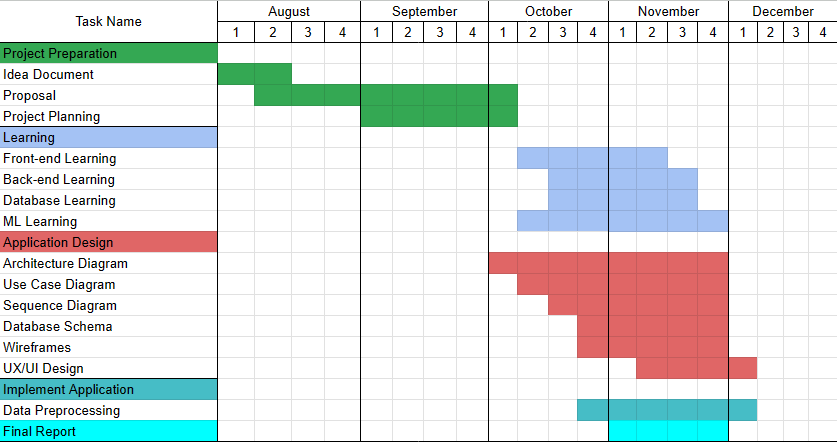
\includegraphics[width=15cm]{./Pictures/Gantt_Chart_1st_Sem.png}}
    \caption{ภาคการศึกษาที่ 1}\label{fig:Gantt_Chart_1st_Sem}
  \end{figure}

  \begin{figure}[!h]\centering
    \setlength{\fboxrule}{0.5mm} % can define this in the preamble
    \setlength{\fboxsep}{0.5cm}
    \fbox{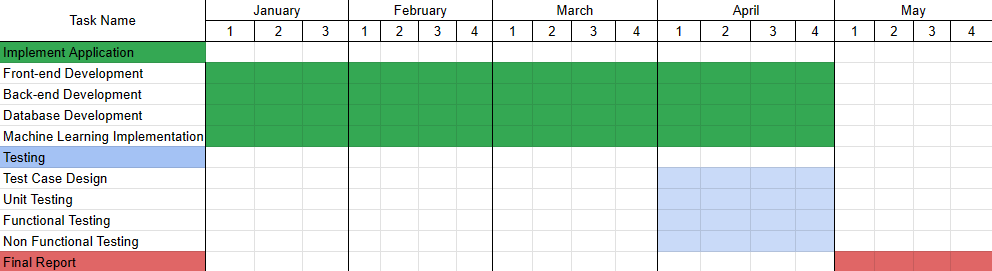
\includegraphics[width=15cm]{./Pictures/Gantt_Chart_2nd_Sem.png}}
    \caption{ภาคการศึกษาที่ 2}\label{fig:Gantt_Chart_2nd_Sem}
  \end{figure}

\newpage

\section{ขอบเขตของโครงงาน}
แอปพลิเคชันสำหรับการแนะนำกิจกรรม และชมรมให้แก่นักศึกษา โดยมีขีดความสามารถดังต่อไปนี้

  \begin{enumerate}
    \item ระบบ Log in ผ่านอีเมลของมหาวิทยาลัย
    \item ระบบรวบรวมข้อมูลของชมรมต่าง ๆ เอาไว้ โดยผู้ใช้สามารถค้นหาและติดตามข้อมูลของชมรมที่ตนเองสนใจได้
    \item ระบบแจ้งเตือนกิจกรรมที่เกี่ยวข้องกับชมรมหรือความสนใจของนักศึกษา
    \item ระบบแจ้งเตือนการประเมินผลกิจกรรม เมื่อฟอร์มการประเมินพร้อมใช้งาน
    \item ระบบแนะนำกิจกรรมและชมรม ตามความสนใจของผู้ใช้โดยอ้างอิงจาก tag ของกิจกรรม
    \item ระบบวิเคราะห์ความสนใจของผู้ใช้ผ่านเนื้อหาของกิจกรรมที่ผู้ใช้เคยเข้าร่วม เข้าไปอ่านรายละเอียด หรือเกี่ยวข้องกับชมรมที่สนใจ
    \item ระบบแยกประเภทกิจกรรมอัตโนมัติโดยวิเคราะห์จากเนื้อหา ออกมาเป็น tag ต่าง ๆ โดยใช้ Machine Learning
  \end{enumerate}

\section{ประโยชน์ที่คาดว่าจะได้่รับ}
  \begin{enumerate}
    \item แอปพลิเคชันที่สนับสนุนการเข้าร่วมกิจกรรมของนักศึกษา และสามารถแนะนำกิจกรรมชมรมที่นักศึกษาน่าจะสนใจได้
    \item การจำแนกประเภทของกิจกรรมของนักศึกษา
  \end{enumerate}

%%%%%%%%%%%%%%%%%%%%%%%%%%%%%%%%%%%%%%%%%%%%%%%%%%%%%%%%%%%%
%%%%%%%%%%%%%%  Literature Review %%%%%%%%%%%%%%%%%%%%%%%%%%
%%%%%%%%%%%%%%%%%%%%%%%%%%%%%%%%%%%%%%%%%%%%%%%%%%%%%%%%%%%%

\chapter{ทฤษฎีความรู้และงานที่เกี่ยวข้อง}
ในบทนี้จะกล่าวถึงรายละเอียดของทฤษฏี ความรู้ และเทคโนโลยีที่นำมาใช้ในการสร้างและพัฒนาแอปพลิเคชัน Actiwiz โดยจะอธิบายความสามารถและการหยิบมาใช้งานในโครงการโดยละเอียด อีกทั้งยังมีการวิเคราะห์ผลิตภัณฑ์ในประเภทเดียวกันที่มีการใช้งานอยู่เพื่อนำมาปรับใช้กับตัวโครงการอีกด้วย

\section{ทฤษฏีและความรู้ที่เกี่ยวข้อง}
  \subsection {การเรียนรู้ของเครื่อง}
  \subsubsection {Content-Based Filtering}
Content-Based Filtering \cite{Content-Based} เป็นหนึ่งในแนวทางที่ได้รับความนิยมอย่างมากในระบบการแนะนำ เนื่องจากความสามารถในการให้คำแนะนำที่มีความเป็นบุคคลและเกี่ยวข้องกับความสนใจของผู้ใช้งาน 
กระบวนการนี้เน้นการวิเคราะห์เนื้อหาที่ผู้ใช้งานมีความสนใจและแนะนำสิ่งที่มีเนื้อหาที่คล้ายคลึงกันให้กับผู้ใช้งาน ตัวอย่างเช่น การแนะนำหนังสือที่มีเนื้อหาใกล้เคียงกับที่ผู้ใช้งานเคยซื้อมาก่อนหน้านี้ 
ดังนั้นเทคนิคนี้จึงเป็นการสร้างคำแนะนำที่เน้นความเป็นบุคคลและความสอดคล้องกับความต้องการของผู้ใช้งานอย่างมีความแม่นยำและเหมาะสม 
อย่างไรก็ตามการทำ Content-Based Filtering นั้น จะยึดตามความสนใจของผู้ใช้งานที่มีประวัติเก็บเอาไว้ทำให้สามารถแนะนำได้ในวงแคบ ๆ เท่านั้น
\subsubsection {Collaborative Filtering}
  Collaborative Filtering \cite{Item-Based}, \cite{Content-Boosted} เป็นหนึ่งในแนวทางที่ได้รับความนิยมอย่างมากในการสร้างคำแนะนำสำหรับผู้ใช้งาน แนวทางนี้เสนอหลักการแนะนำที่มาจากพฤติกรรมการใช้งานที่เกิดขึ้นก่อนหน้านี้ของผู้ใช้งาน 
  การ Collaborative Filtering มีวิธีการหลักที่สำคัญสองวิธีคือ \\
  User-Based Collaborative Filtering: แนวทางนี้จะทำการแนะนำสิ่งที่ผู้ใช้งานมีความสนใจอยู่ หากมีความคล้ายคลึงในพฤติกรรมการใช้งานระหว่างผู้ใช้งานสองคน 
  เช่น ถ้าผู้ใช้งานสองคนมีรูปแบบพฤติกรรมที่คล้ายกัน ระบบจะแนะนำสิ่งที่ผู้ใช้อีกคนเคยใช้งานให้กับผู้ใช้งานคนอื่น ซึ่งเพิ่มโอกาสที่จะให้คำแนะนำที่หลากหลายขึ้นได้ 
  อย่างไรก็ตามก็อาจมีโกาสที่จะแนะนำสิ่งที่ผู้ใช้งานไม่สนใจเลยได้เช่นกัน และยังมีปัญหาความซับซ้อนเกิดขึ้นได้หากมีผู้ใช้งานหรือสิ่งที่จะแนะนำเป็นจำนวนมาก \\
  Item-Based Collaborative Filtering: แนวทางนี้จะทำการแนะนำสิ่งที่ผู้ใช้งานมีความสนใจ และจะทำการแนะนำสิ่งที่มีเนื้อหาคล้ายกัน เมื่อพิจารณาการกระทำที่เกิดขึ้นก่อนหน้านี้ 
  ระบบจะแนะนำสิ่งที่มีความคล้ายคลึงให้กับผู้ใช้งาน อย่างไรก็ดีเนื่องจากเป็นการแนะนำจากสิ่งที่มีความใกล้เคียงกัน คำแนะนำที่ได้จึงอาจไม่ใช่สิ่งที่ผู้ใช้งานมองหา \\
\subsubsection {การประมวลผลภาษาธรรมชาติ}
การประมวลผลภาษาธรรมชาติ (Natural Language Processing หรือ NLP) \cite{recommendation}, \cite{NLPforContentbase} เป็นสาขาหนึ่งของปัญญาประดิษฐ์ ที่จะมุ่งเน้นการให้ความสามารถแก่คอมพิวเตอร์ที่เป็นการเข้าใจ ตีความ และปฏิสัมพันธ์กับภาษาของมนุษย์ 
แนวทางนี้นำเอาอัลกอริทึมและเทคนิคในการประมวลผล วิเคราะห์ และสร้างข้อมูลข้อความและเสียง เพื่อให้เครื่องคอมพิวเตอร์สามารถสกัดความหมาย บริบท และความรู้จากภาษาที่มนุษย์สร้างขึ้นได้ \\
  \subsubsection {Word Embedding}
	 Word Embedding \cite{WordEmbedding}, \cite{WordEmbeddingForCollaborative} ในการทำการประมวลผลภาษาธรรมชาติคือการที่แปลงคำต่าง ๆ ออกมาเป็นเวคเตอร์เพื่อที่จะตรวจสอบความหมายของคำและความหมายในการสร้างประโยค 
   ซึ่งเป็นพื้นฐานในการทำโมเดลการประมวลผลภาษาธรรมชาติซึ่งสามารถนำมาประยุกต์ได้ทั้งการที่จะจัดประเภทกิจกรรมหรือการวิเคราะห์ความต้องการของผู้ใช้งานจากข้อความที่ถูกใช้ \\

\newpage

  \subsubsection {Transformer Model}
   Transformer Model \cite{Transformers} คือสถาปัตยกรรมการเรียนรู้ของเครื่องสำหรับการประมวลผลและทำความเข้าใจภาษาของมนุษย์ ซึ่งทำงานได้ดีในการแปลภาษา การสรุป และการสร้างข้อความ 
   โดยอาศัยหลักการของ self-attention ในการทำความเข้าความสัมพันธ์ระหว่างคำในประโยคพร้อมกัน ทำให้สามารถเข้าใจบริบทและความหมายได้มากขึ้นอย่างมีประสิทธิภาพ 
   โดย Transformer-base model ที่ถูกใช้งานในโครงงานนี้ มี 2 รูปแบบ คือ 
   
   \begin{enumerate}
   \item mT5 (Text-to-Text Transfer Transformer) เป็นสถาปัตยกรรมที่ประยุกต์มาจาก unified text-to-text framework ซึ่งพัฒนาจาก NLP model หลากหลายงานให้ใช้งานง่ายขึ้น จึงสามารถนำมา train ต่อเพื่อทำงานเกี่ยวกับ Natural language processing ได้อย่างเอนกประสงค์ โดยที่มีผลกระทบต่อประสิทธิภาพในการทำงานเพียงเล็กน้อย อย่างไรก็ตาม T5 มีข้อจำกัดในการเข้าใจบริบทของข้อความและต้องอาศัยการปรับแต่งในการทำงานที่เฉพาะด้าน
   \item BERT (Bidirectional Encoder Representations from Transformers) \cite{BERT}  สถาปัตยกรรมที่ถูก train โดยคลังข้อความขนาดใหญ่ จึงสามารถทำงานในการจับบริบทที่อยู่เบื้องหลังข้อความได้ เหมาะกับการทำงาน Natural language processing ที่หลากหลาย อย่างไรก็ตาม BERT ต้องการหน่วยประมวลผลในการ train และใช้งาน รวมไปถึงไม่สามารถปรับแต่งได้เอนกประสงค์เท่า T5 
   \end{enumerate} 
   
   \subsubsection {โครงข่ายประสาทเทียม}
   โครงข่ายประสาทเทียม (Artificial neural network) เป็นสถาปัตยกรรมการเรียนรู้ของเครื่องที่ได้รับแรงบันดาลใจมาจากระบบประสาทของมนุษย์ โดยมีหลักการคือการแบ่งการทำงานเป็น node ต่าง ๆ 
   ที่รับค่าที่ประมวลผลมาจาก node ที่อยู่ใน input layer แล้วส่งต่อให้ node ประมวลผลที่อยู่ใน hidden layer ไปเรื่อย ๆ จนถึง node ประมวลผลสุดท้ายใน output layer 
   เพื่อตีความผลลัพธ์ ซึ่งสามารถทำงานได้หลากหลายรวมไปถึงงานการประมวลผลภาษาธรรมชาติซึ่งในโครงงานนี้มี โครงข่ายประสาทเทียม 2  รูปแบบ คือ
   
    \begin{enumerate}
      \item Shallow Neural Network ซึ่งเป็น Neural Network ที่มีจำนวน Layer ในการประมวลผลอยู่น้อย มีข้อดีคือการที่จะใช้หน่วยประมวลผลน้อยและสามารถ train ได้ไว แต่ในทางกลับกันก็มีข้อจำกัดในการตีความที่ซับซ้อนรวมถึงบริบทที่อยู่ในข้อความของงาน Natural Language Processing
      \item Regularizing and Optimizing LSTM Language Model \cite{LSTM} คือ Neural Network ที่ถูกพัฒนามาสำหรับการทำ Natural Language Processing ทำให้สามารถประมวลผลข้อมูลที่มีความต่อเนื่องอย่างเช่นประโยคได้ ตัวโมเดลมีความสามารถในการทำความเข้าใจบริบทในข้อความได้ โดยพิจารณาข้อมูลในหน่วยความจำของโมเดล ซึ่งสามารถจดจำหรือลบข้อมูลได้ตามความเหมาะสม และสามารถรับมือกับข้อความที่ไม่รู้จักได้ดี อย่างไรก็ตามคุณภาพของ model ขึ้นอยู่กับคุณภาพของข้อมูลที่ใช้ train และการปรับแต่งค่อนข้างส่งผลกับตัว model
    \end{enumerate}
   
   \newpage
   \subsection { สถาปัตยกรรมของแอปพลิเคชันในโทรศัพท์ \cite{MobileAppArchitecture}} 
   ในการพัฒนาแอปพลิเคชัน สถาปัตยกรรมหมายถึงกฎ กระบวนการ และโครงสร้างภายในของแอปพลิเคชัน หรือก็คือวิธีการสร้างแอปพลิเคชัน โดยจะเป็นการกำหนดรูปแบบที่ส่วนประกอบต่าง ๆ สื่อสารกันเพื่อประมวลผลข้อมูล input จากผู้ใช้และประมวลผลข้อมูล output ให้กับผู้ใช้ โดยมีตัวอย่างสถาปัตยกรรมดังรูปที่ \ref{fig:mobile_arc1}

    \begin{figure}[!h]\centering
      \setlength{\fboxrule}{0.5mm} % can define this in the preamble
      \setlength{\fboxsep}{0.5cm}
      \fbox{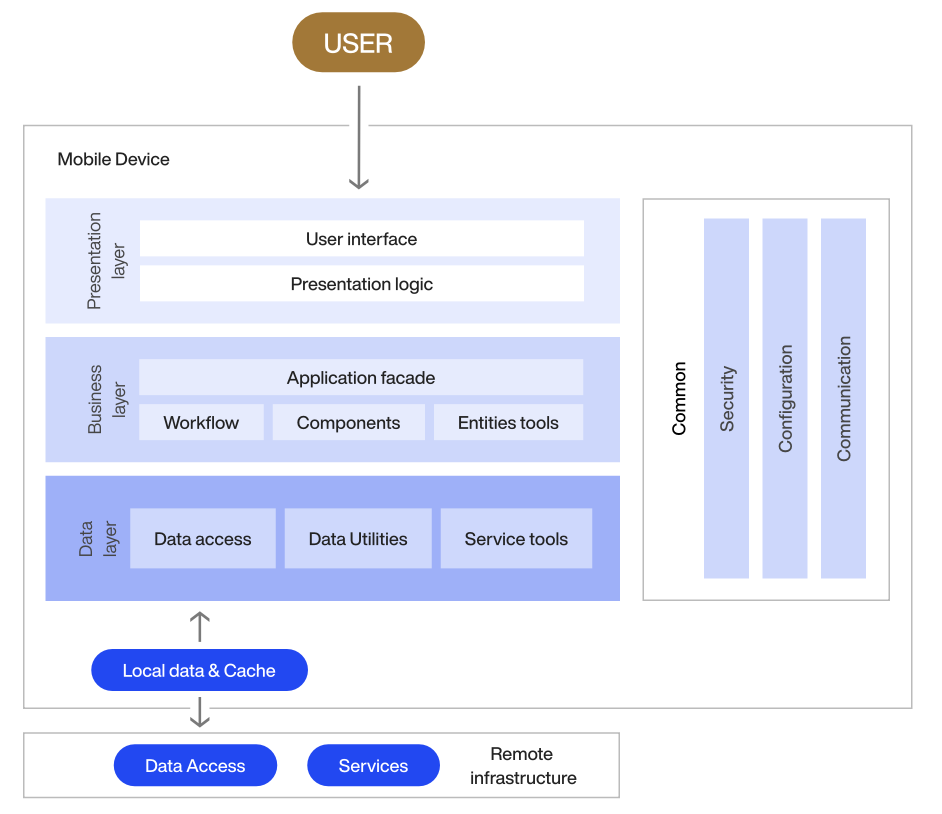
\includegraphics[width=12cm]{./Pictures/Mobil_Arc.png}}
      \caption{Mobile Application Architecture \cite{MobileAppArchitectureOverview}}\label{fig:mobile_arc1}
    \end{figure}

สถาปัตยกรรมของแอปพลิเคชันส่วนใหญ่จะประกอบด้วยสามเลเยอร์หลัก ๆ ได้แก่ Presentation layer, Business layer และ Data layer
  \begin{enumerate} 
    \item Presentation layer\cite{MobileAppArchitecture} \\
          หรือก็คือ front end เป็นส่วนของแอปพลิเคชันที่ผู้ใช้มองเห็นและมีปฏิสัมพันธ์ด้วยได้ โดยมีส่วนติดต่อผู้ใช้ (user interface หรือ UI) ของแอปพลิเคชันเป็นส่วนสำคัญของเลเยอร์นี้
          วัตถุประสงค์หลักของเลเยอร์นี้คือการนำข้อมูลที่ส่งมาจาก business layer มาแสดงผลในลักษณะที่ผู้ใช้สามารถเข้าใจได้
          ไม่ว่าจะเป็น UI แบบพื้นฐาน เช่น UI แสดงที่อยู่อีเมลของผู้ใช้หรือ UI ที่ซับซ้อน เช่น แอปซื้อขายหุ้นซึ่งแสดงข้อมูลสดเกี่ยวกับตลาดหลักทรัพย์ออกมาแสดงเป็นกราฟหรือแผนภูมิ แม้ว่านักพัฒนาส่วนใหญ่จะรับผิดชอบ Business layer และ Data layer

      \begin{figure}[!h]\centering
        \setlength{\fboxrule}{0.5mm} % can define this in the preamble
        \setlength{\fboxsep}{0.5cm}
        \fbox{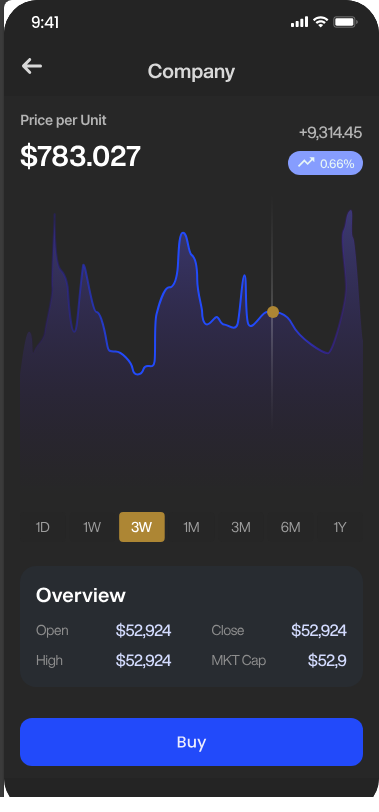
\includegraphics[width=4cm]{./Pictures/Mobile_Arc2.png}}
        \caption{Presentation layer \cite{PresentationLayer}}\label{fig:mobile_arc2}
      \end{figure}

\newpage

    \item Business layer \cite{MobileAppArchitecture} \\
          เลเยอร์นี้จะประกอบด้วยตรรกะหลักของแอปพลิเคชัน หรือก็คือวิธีการทำงานของแอปพลิเคชัน โดยมักจะเป็นการนำข้อมูลที่ผู้ใช้ป้อนหรือข้อมูลจาก Data layer มาประมวลผล จากนั้นจึงส่งไปยัง presentation layer
          ส่วนใหญ่ business layer จะเป็นส่วนที่ซับซ้อนที่สุดในแอปพลิเคชัน 
          โดยปกติแล้วจะแบ่งออกเป็น Layer ย่อยๆหรือส่วนประกอบหลายส่วน โดยแต่ละส่วนมีหน้าที่รับผิดชอบในการทำงานเฉพาะ
          ตัวอย่างเช่น หากคุณมีแอปการจัดการทรัพยากรองค์กร (ERP) business layer อาจมีส่วนประกอบสำหรับการจัดการคลังสินค้าและระบบจัดการสินค้าคงคลัง 

      \begin{figure}[!h]\centering
        \setlength{\fboxrule}{0.5mm} % can define this in the preamble
        \setlength{\fboxsep}{0.4cm}
        \fbox{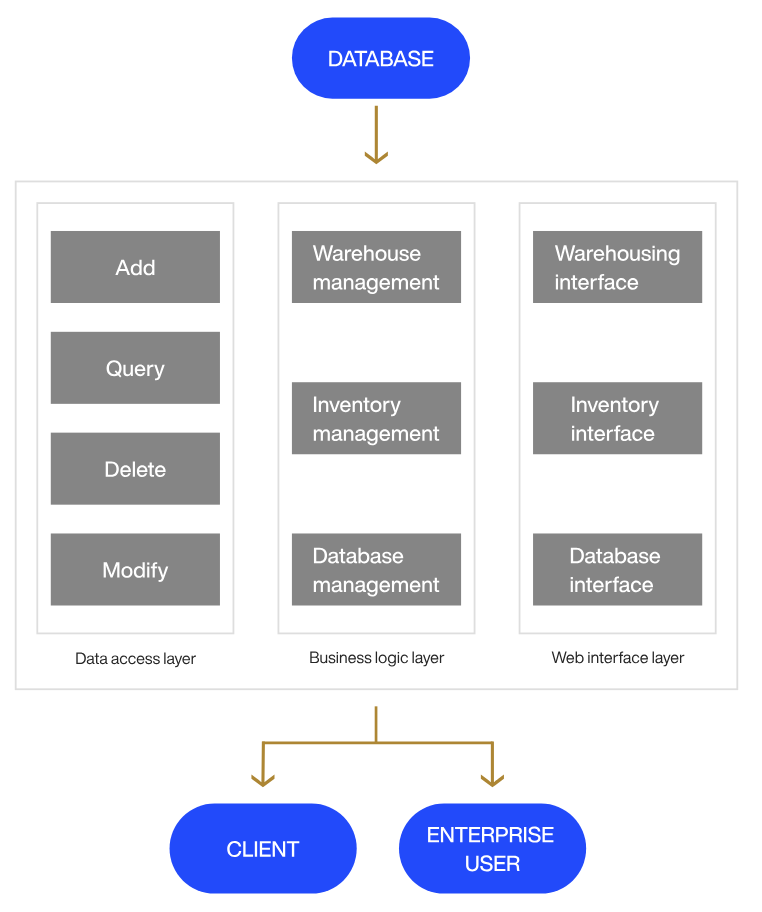
\includegraphics[width=11cm]{./Pictures/Business_layer.png}}
        \caption{Business layer \cite{BusinessLayer}}\label{fig:business_layer}
      \end{figure}
\newpage
    \item Data layer \\
          Data Layer \cite{MobileAppArchitecture} นี้เป็นตัวกลางระหว่าง Layer อื่นๆ กับทรัพยากรภายนอก
          วัตถุประสงค์หลักของ Layer นี้คือการรวบรวมข้อมูลจากแหล่งต่าง ๆ เช่น ฐานข้อมูล, เซิร์ฟเวอร์คลาวด์ หรือ API แล้วส่งไปยัง Layer ด้านบน 
          ตัวอย่างเช่น เมื่อผู้ใช้ขอให้แอปพลิเคชันแสดงโปรไฟล์ของตน data layer จะเชื่อมต่อกับ Database และขอข้อมูลที่เกี่ยวข้องทั้งหมด เช่น ชื่อ วันเกิด ไฟล์รูปภาพ และอื่นๆ อย่างไรก็ตามใน layer นี้ข้อมูลส่วนใหญ่ยังไม่ผ่านการประมวลผล จึงอาจจะมีข้อมูลบางอย่าง เช่น แท็กหรือไอดีที่ผู้ใช้ไม่ควรเห็น ในส่วนนี้จึงต้องทำการส่งข้อมูลให้ business layer ประมวลผลเพิ่มเติมเป็นลำดับต่อไป
    \end{enumerate}

\subsection {HTTP Protocol} 
  \subsubsection {HTTP Protocol คืออะไร}
    HTTP \cite{HTTPProtocol} (Hypertext Transfer Protocol) เป็นโปรโตคอลที่ใช้ในการแลกเปลี่ยนข้อมูลผ่านทางอินเทอร์เน็ต เปรียบเสมือนระบบส่งข้อมูลบนอินเทอร์เน็ตที่ช่วยให้มั่นใจได้ว่าข้อมูลจะถูกส่งจากที่หนึ่งไปยังอีกที่หนึ่งได้ 
  
\newpage 

    \subsubsection {HTTP Request-Response Cycle}

    \begin{figure}[!h]\centering
      \setlength{\fboxrule}{0.5mm} % can define this in the preamble
      \setlength{\fboxsep}{0.3cm}
      \fbox{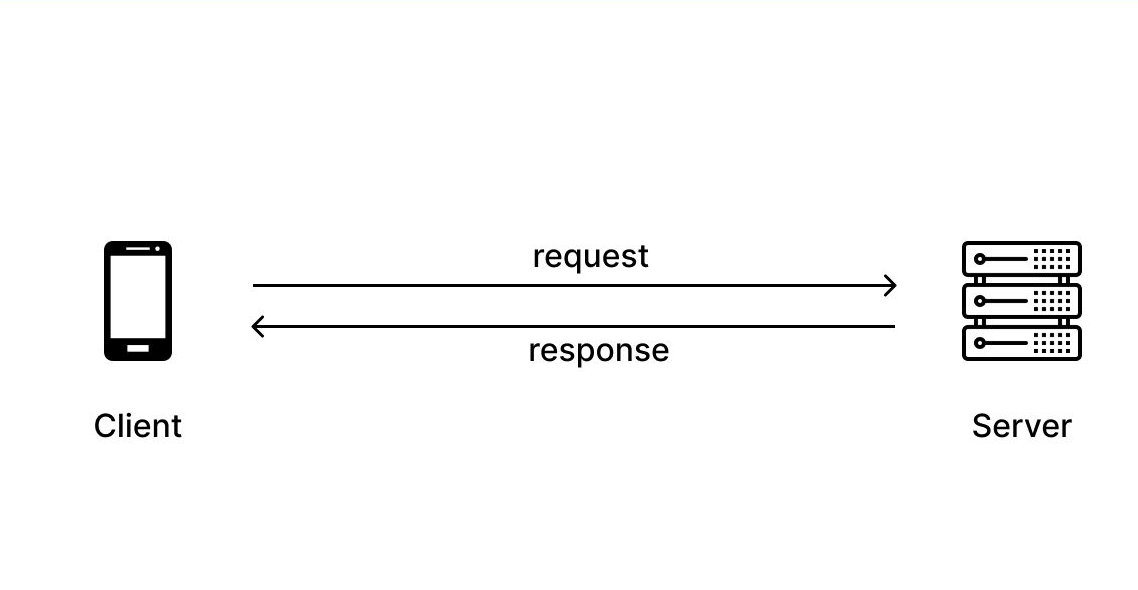
\includegraphics[width=10cm]{./Pictures/HTTP.png}}
      \caption{HTTP Request-Response Cycle \cite{HTTPCycle}}\label{fig:http}
    \end{figure}


การสื่อสารในโปรโตคอล HTTP มีศูนย์กลางอยู่ที่แนวคิดที่เรียกว่า Request-Response Cycle เป็นกระบวนการที่ไคลเอนต์ (Client) เช่น เว็บเบราว์เซอร์หรือแอปพลิเคชันมือถือ สื่อสารกับเซิร์ฟเวอร์ (Server) เพื่อขอทรัพยากรที่ต้องการหรือเพื่อดำเนินการบางอย่าง โดยวงจรประกอบด้วยหลายขั้นตอนได้แก่ \\
    \begin{enumerate}
      \item ไคลเอนต์เริ่มต้นการส่งคำขอไปยังเซิร์ฟเวอร์โดยการส่งข้อความร้องขอ (HTTP request message) ซึ่งประกอบด้วยข้อมูลอาทิเช่นทรัพยากรที่ต้องการและพารามิเตอร์เพิ่มเติมอื่น ๆ
      \item เซิร์ฟเวอร์ได้รับข้อความร้องขอและประมวลผลโดยใช้ทรัพยากรที่มีอยู่เพื่อสร้างข้อความตอบกลับ (HTTP response message)
      \item เซิร์ฟเวอร์ส่งข้อความตอบกลับไปยังไคลเอนต์ ซึ่งโดยทั่วไปจะมีทรัพยากรที่ร้องขอ (เช่น หน้าเว็บ) และข้อมูลเพิ่มเติมหรือเมทาดาตา (ข้อมูลที่ใช้อธิบายชุดข้อมูลอื่นอีกที)
      \item ไคลเอนต์ได้รับข้อความตอบกลับและประมวลผล โดยปกติจะเป็นการแสดงเนื้อหาในเว็บเบราว์เซอร์หรือในแอปพลิเคชัน
      \item ไคลเอนต์อาจเริ่มการร้องขอเพิ่มเติมไปยังเซิร์ฟเวอร์ โดยทำซ้ำขั้นตอนเดิมแล้วแต่ความจำเป็น
    \end{enumerate}

\subsubsection {HTTP Request Methods}
Request method จะเป็นการบอกเซิร์ฟเวอร์ว่าลูกค้าต้องการให้เซิร์ฟเวอร์ดำเนินการอะไร 
Request method ที่พบเจอบ่อยจะมีดังนี้ \\

\begin{table}[!h]\centering
  \begin{tabular}{|
  >{\columncolor[HTML]{FFFFFF}}c |c|}
  \hline
  \cellcolor[HTML]{6D9EEB}HTTP METHODS & \cellcolor[HTML]{6D9EEB}DEFINITION                \\ \hline
  {\color[HTML]{0A0A23} HEAD} & \cellcolor[HTML]{FFFFFF}ถามเซิร์ฟเวอร์เกี่ยวกับสถานะ (ขนาด ความพร้อมใช้งาน) ของทรัพยากร \\ \hline
  {\color[HTML]{0A0A23} GET}           & ขอทรัพยากรจากเซิร์ฟเวอร์                          \\ \hline
  {\color[HTML]{0A0A23} POST}          & ขอให้เซิร์ฟเวอร์สร้างทรัพยากรใหม่                 \\ \hline
  {\color[HTML]{0A0A23} PUT}           & ขอให้เซิร์ฟเวอร์แก้ไข/อัปเดตทรัพยากรที่มีอยู่แล้ว \\ \hline
  {\color[HTML]{0A0A23} DELETE}        & ขอให้เซิร์ฟเวอร์ลบทรัพยากร                        \\ \hline
  \end{tabular}
    \caption{\centering HTTP Request Methods}\label{tab:HTTP Request Methods}
\end{table}

\newpage

\FloatBarrier
  \subsection {REST API} 
    \subsubsection {REST คืออะไร}
      REST \cite{RestAPI} ย่อมาจาก Representational State Transfer เป็นรูปแบบการส่งข้อมูลระหว่าง Server-Client รูปแบบหนึ่งซึ่งอยู่บนพื้นฐานของ HTTP Protocol เป็นการสร้าง Web Service เพื่อแลกเปลี่ยนข้อมูลกันผ่าน Application วิธีหนึ่ง ซึ่งส่งข้อมูลได้หลายชนิด ไม่ว่าจะเป็น Text, XML, JSON หรือส่งมาเป็นหน้า HTML เลย
      REST ทำงานอยู่บน HTTP Protocol ทำให้เวลาใช้งานจะต้องอยู่บนพื้นฐาน HTTP Method เช่น GET, POST, PUT, DELETE จะใช้ Method ไหนก็ขึ้นอยู่กับว่าจะทำอะไรกับข้อมูล แต่ก็ต้องควรใช้คู่กับ Operation CURD เช่น เมื่อต้องการจะเรียกดูข้อมูลทั้งหมดก็ใช้ GET เมื่อต้องการเพิ่มข้อมูลก็ใช้ POST เป็นต้น 

    \subsubsection {การออกแบบ REST API \cite{RestAPIDesign}}

      \begin{enumerate}
        \item เลือกใช้ HTTP Method ให้เหมาะสมกับการใช้งาน
              ในกรณีปกติ การสร้าง URL จะไม่ใส่ชื่อกิริยาของ API มาอยูใน path เช่น /createUsers, /getUserDetail นั้นผิดหลักในการสร้าง เนื่องจากในการที่จะระบุว่าแต่ละ API จะถูกใช้ทำหน้าที่อะไรนั้นจะมี HTTP Method ในการระบุอยู่แล้ว 
        \item การสร้าง URL ของ API endpoint ให้ตรงตามมาตรฐานในการสร้าง URL ของ API นั้นมีทั้งหมดสามกฎที่สำคัญ ก็คือ

        \begin{itemize}
          \item ควรจะมีแค่ชื่อ resource เท่านั้น เนื่องจาก resource เป็นตัวแทนของ สิ่งของบางอย่าง ที่เชื่อมโยงกับข้อมูล เช่น Users, Customers, Orders
          \item ชื่อ path ควรจะเป็นรูปพหูพจน์ของ resource 
          \item ไม่ควรจะมีชื่อกิริยาที่บอกถึงวัตถุประสงค์ของ API (เช่น add, update, delete) ตามที่กล่าวในข้อแรก
        \end{itemize}
      
สมมติว่าต้องการ API ที่เกี่ยวข้องกับ Users โดยการสามารถ สร้างข้อมูล user, แก้ไขข้อมูล user, แสดงข้อมูล user และ ลบข้อมูล user สามารถเขียนออกมาได้ดังนี้
      
        \begin{itemize}
          \item method: POST path: /users สร้างข้อมูล user ใหม่
          \item method: PUT path: /users/99 จะแก้ไขข้อมูล user ที่ id 99
          \item method: GET path: /users จะได้ข้อมูลของ user ทั้งหมด
          \item method: GET path: /users/99 จะได้รายละเอียดของ user ที่ id 99
          \item method: DELETE path: /users/99 จะเป็นการลบข้อมูล user ที่ id 99
        \end{itemize}

กรณีที่ข้อมูลความเกี่ยวข้องกัน ส่วนใหญ่จะใช้เป็น Nested endpoint แทน query string เช่น ต้องการข้อมูลของ user ทั้งหมดที่อยู่ใน customer id เป็น 2 สามารถเขียนเป็น GET /customers/2/users 
แต่มีบางกรณีที่ ข้อมูล Nested ที่เยอะมากๆจนหากใช้งานเป็น URL path จะมียาวมากเกินไป อาจจะใส่เป็น query string หรือ ใส่ใน body แทน เพื่อให้อ่านได้ง่ายขึ้น ซึ่งต้องพิจารณาถึง use case ด้วย
  
        \item ควรมี API Versioning
              หาก API มีผู้ใช้เข้ามาใช้งานแล้ว ในการแก้ไขสิ่งที่มีขนาดใหญ่ ก็จะทำได้ลำบากขึ้น เพราะถ้าแก้ไปแล้ว ทำให้ service ที่ใช้ API อยู่ใช้งานไม่ได้อาจจะทำให้เกิดปัญหาขึ้น เพราะอย่างนั้น ทุก ๆ API ควรทำ version ไว้ หากมีการเปลี่ยนแปลงก็สามารถแยกออกมาเป็นอีก version ได้เลย โดยทั้ง version เก่าและใหม่ต้องทำงานได้ทั้งคู่ ตัวอย่างเช่น
              POST v1/users และ POST v2/users สามารถนำเลข version มาต่อหน้า API ได้เลย

        \item การตั้งชื่อ (Naming Conventions) ให้สัมพันธ์กันทั้งระบบ
              การตั้งชื่อตัวแปร (ของ body และ response) ที่พบเจอบ่อยที่สุดจะเป็น camel case, snake case เป็น key ซึ่งสามารถเลือกใช้ได้ตามใจชอบ แต่ควรตั้งชื่อให้เหมือนกันทั้งระบบ

        \item ใช้งาน parameters ให้เหมาะสม parameters คือ query ที่ต่อท้าย URL path ซึ่งจะมี action ต่าง ๆ ดังนี้
          \begin{itemize}
            \item Filtering (การกรองข้อมูล) สามารถกรองข้อมูลแบบมีเงื่อนไขได้ โดย จะส่งผ่านมาทาง query ที่ต่อท้าย URL path เช่น GET /orders?name=MyOrders\&customerId=2
                  ผลลัพธ์หลัง filter คือข้อมูลของ order ที่มีชื่อว่า “MyOrders” และอยู่ใน customer id ที่ 2 จากหลักการข้อ 2. ที่กล่าวไปว่า ข้อมูล Nested ที่เยอะมาก ๆ หรือต้องการกรองข้อมูลจำนวนมาก ถ้าเอามาเป็น URL path จะมีความยาวเกินไป สามารถนำมาใส่ใน filter ต่อท้าย URL path แทนได้
            \item Sorting (การจัดเรียงข้อมูล) สามารถเรียงลำดับข้อมูลที่เรียกมาแสดงผลได้ ซึ่งการออกแบบ sort ที่ดีจะต้องออกแบบให้ยืดหยุ่น สามารถเรียงจากน้อยไปมาก หรือมากไปน้อยได้ โดยใส่ query เข้าไปต่อท้าย path คล้ายกับ filter ซึ่งสามารถนำ sort by ไปต่อท้ายได้ เช่น
                  GET /users?sort by=+email หรือ GET /users?sort by=-email จากตัวอย่างด้านบน +email คือการเรียงจากน้อยไปมาก และ -email เรียงจากมากไปน้อย หรือสามารถเขียนในรูปแบบอื่นๆ ได้เช่น
                  \begin{itemize} 
                    \item GET /users?sort by=asc(email) หรือ GET /users?sort by=desc(email)
                    \item GET /users?sort by=email.asc หรือ GET /users?sort by=email.desc
                    \item GET /users?sort by=email\&order by=asc หรือ GET /users?sort by=email\&order by=desc
                  \end{itemize}

      \end{itemize}

โดยหลักสำคัญจะอยู่ที่ทุกรูปแบบการเขียนจะต้องหยืดหยุ่น สามารถเปลี่ยนลำดับการเรียงข้อมูลได้ และผู้ใช้งานสามารถอ่านได้อย่างเข้าใจว่าเป็นการเรียงลำดับแบบไหน

          \begin{itemize} 
            \item Searching (การค้นหาข้อมูล) หลักการจะค่อนข้างคล้าย filter คือการค้นหาข้อมูลแบบมีเงื่อนไข เมื่อต้องการค้นหาข้อมูล จะส่งผ่านมาทาง query ต่อท้าย String ตัวอย่างเช่น เมื่อต้องการค้นหาชื่อของ order ที่ชื่อว่า “THAIPOST1234” ในระบบ จะส่งผ่านทาง query params ตามตัวอย่างด้านล่าง
              GET /orders?search='THAIPOST1234' \\ 
            \item Pagination (การจัดแบ่งหน้า) \cite{Pagination} สามารถจัดหน้าของข้อมูลได้ในกรณีที่ข้อมูลมีจำนวนมาก
          \end{itemize}

            \begin{figure}[!h]\centering
              \setlength{\fboxrule}{0.5mm} % can define this in the preamble
              \setlength{\fboxsep}{0.5cm}
              \fbox{
\includegraphics[width=10cm]{./Pictures/google.png}}
              \caption{tab เลือกหน้าของ Google}\label{fig:google}
            \end{figure}

ตัว paginate จะช่วยย่อยข้อมูลออกมาเป็นก้อนเล็ก ๆ โดยสามารถโยน query เพื่อระบุหน้า จำนวนข้อมูลที่ต้องการแสดงได้ เช่น GET /orders?page=2\&limit=50
ผลลัพธ์ที่ได้จะเป็นข้อมูลตัวที่ 51–100 นั้นเอง เพราะเป็น page ที่ 2 ข้อมูลจำนวน 50 ตัว

        \item ใช้ HTTP Status code ให้ตรงตามความหมาย
              หลังจากที่ฝั่งผู้ใช้งาน API (Client) ส่ง request ไปหา server ผ่าน API แล้วฝั่ง Client จะต้องทำการยืนยันให้ได้ว่า API ใช้งานได้จริงหรือไม่ หรือส่งไปสำเร็จไหม จึงมีการต้องส่ง response ที่มี HTTP Status code ระบุ กลับไปยัง client เพื่อบอกว่า request นั้น ๆ Pass, Fail หรือ request นั้นผิด
              กรณี Success จะมี HTTP status code ที่ใช้งานกันทั่วไปได้แก่ 
          \begin{itemize}
            \item 200 Ok: เป็นมาตรฐานของ HTTP response เพื่อบ่งบอกว่า request นั้นสำเร็จ ใช้สำหรับ GET, PUT หรือ POST ก็ได้
            \item 201 Created: เป็น response เพื่อบ่งบอกว่าข้อมูลใหม่ได้ถูกสร้างขึ้นสำเร็จ ใช้สำหรับ POST
            \item 204 No Content: เป็น response สำหรับบ่งบอกดำเนินการ Success แต่ไม่ได้ return ข้อมูลกลับ ส่วนใหญ่จะใช้กรณีลบข้อมูล DELETE ที่ไม่ได้ส่ง response ที่เป็นข้อมูลกลับไป
                  กรณี Error จะมี HTTP status code ที่ใช้งานกันทั่วไปได้แก่
            \item 400 Bad Request: status นี้จะบ่งบอกว่า request ที่ส่งมาโดย client นั้นไม่มี action ใดๆ และ Server ไม่เข้าใจ เช่น JSON ผิด หรือ parameters ไม่ถูกต้อง
            \item 401 Unauthorized: เป็น response ที่บ่งบอกว่า client ไม่ได้รับอนุญาตในการเข้าถึง อาจจะเป็นกรณีที่ใส่ token ผิด หมดอายุ หรือไม่ได้แนบ token มา
            \item 403 Forbidden: เป็น response ที่บ่งบอกว่า client ได้รับการอนุญาตในการเข้าถึงระบบ (login ผ่าน) แต่จะมีข้อมูลบางหน้า ที่ไม่มีสิทธิ์ในการเข้าถึง
            \item 404 Not Found: เป็น response ที่บ่งบอกว่า request นั้นไม่ว่างใช้งานตอนนี้ หรือ request ที่เรียกนั้นไม่มีอยู่ในระบบ
            \item 405 Gone: เป็น response ที่บ่งบอกว่า resource ที่ต้องการนั้นไม่มี หรือถูกย้ายไป
            \item 429 Too many Request: เป็น response ที่บ่งบอกว่า request นั้นติด limit ใช้กรณีที่กำหนด rate limit ไว้ว่า API นั้น ๆ จะสามารถเรียกได้กี่ครั้ง
            \item 500 Internal Server Error: เป็น response ที่บ่งบอกว่าการ request นั้นถูกต้องแล้ว แต่ server พังเอง ซึ่งอาจจะพังที่ตัวโค้ดของระบบเอง
            \item 503 Service Unavailable: เป็น response ที่บ่งบอกว่า server ใช้การไม่ได้ (ระบบพัง) โดย Server จะไม่สามารถรับ request ที่ส่งเข้ามาได้
            \item 504 Bad Gateway Gateway Timeout: เป็น response ที่บ่งบอกว่า web server อย่างพวก nginx หรือ apache พัง
                  จะเห็นว่า HTTP Status code แต่ละตัวจะมีความหมายของของตัวเองชัดเจน เพราะฉะนั้นการออกแบบที่ดีจะต้องเลือกให้ HTTP Status code ให้ตรงตามวัตถุประสงค์เพื่อให้ผู้ใช้งานที่ได้รับ response กลับไป เข้าใจ response นั้นได้ดีมากขึ้น \\
          \end{itemize}
        \item การ Handle Error ให้ user เข้าใจ
              นอกเหนือจาก HTTP Status code แล้ว ต้องออกแบบ response สำหรับ error กรณีต่าง ๆ ไว้ด้วย เพื่อให้ user เข้าใจ error ของ API มากขึ้น ยกตัวอย่างกรณีที่ request ส่งบาง parameter มาไม่ถูกต้อง แทนที่จะ response กลับไปว่า
      \end{enumerate}

  \begin{figure}[!h]\centering
    \setlength{\fboxrule}{0.5mm} % can define this in the preamble
    \setlength{\fboxsep}{0.5cm}
    \fbox{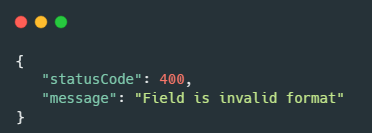
\includegraphics[width=9cm]{./Pictures/Error1.png}}
    \caption{Handle Error1}\label{fig:Error1}
  \end{figure}

โหนดเป็นเหมือน entity ของกราฟสามารถที่จะเก็บ attribute จำนวนมากได้ สำหรับกราฟเราจะเรียก attribute ว่าคุณสมบัติ
ความสัมพันธ์หมายถึงความสัมพันธ์ที่เชื่อมระหว่าง 2 โหนด และเหมือนกับโหนดซึ่งสามารถเก็บคุณสมบัติได้ \\

\newpage

  \begin{figure}[!h]\centering
    \setlength{\fboxrule}{0.5mm} % can define this in the preamble
    \setlength{\fboxsep}{0.5cm}
    \fbox{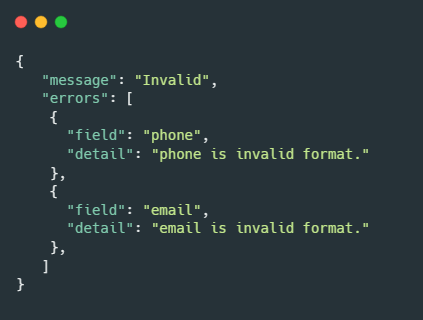
\includegraphics[width=10cm]{./Pictures/Error2.png}}
    \caption{Handle Error2}\label{fig:Error2}
  \end{figure}

การส่งไปในรูปแบบดังกล่าวจะทำให้ user เข้าใจได้เลยว่ามี field ใดที่ผิด format



\subsection {Graph Database} 
  \subsubsection {Graph Database คืออะไร}
    Graph database \cite{GraphDatabase} หรือฐานข้อมูลแบบกราฟ จัดเป็น NoSQL Database รูปแบบหนึ่ง ซึ่งนำมาใช้แก้ปัญหา database ที่มีข้อมูลขนาดใหญ่และไม่มีรูปแบบชัดเจน
    ฐานข้อมูลแบบ Graph ออกแบบมาเพื่อแสดงความสัมพันธ์ (Relationship) ระหว่างข้อมูลที่มีความเชื่อมโยงกับข้อมูลที่เราสนใจได้อย่างชัดเจน รวมถึงมีความสามารถในการเก็บข้อมูลที่ไม่ต้องกำหนดรูปแบบล่วงหน้า
  \subsubsection {ทำไมต้องเป็น Graph Database}
    การเข้าถึง node และ relationships ในฐานข้อมูล Graph เป็นวิธีที่มีประสิทธิภาพและใช้เวลาในการทำงานคงที่ และช่วยให้เราสำรวจการเชื่อมต่อหลายล้านต่อวินาทีต่อเรคคอร์ดได้อย่างรวดเร็ว
    มีความเป็นอิสระจากขนาดรวมของชุดข้อมูลทั้งหมดของเรา ทำให้ฐานข้อมูลแบบ Graph มีความสามารถในการจัดการข้อมูลที่มีรูปแบบซับซ้อนและมีความเชื่อมต่อกันสูงได้มีประสิทธิภาพ 

  \subsubsection {Property ของ Graph Model \cite{GraphDatabaseProperty}} 
    เทคโนโลยีส่วนใหญ่มีวิธีการที่แตกต่างกันเล็กน้อยในการสร้าง องค์ประกอบที่สำคัญของฐานข้อมูล Graph วิธีหนึ่ง คือ Graph Model ข้อมูลจะถูกจัดระเบียบเป็น node, relationship และ properties(ข้อมูลที่อยู่บน node หรือ relationship)

    \begin{figure}[!h]\centering
      \setlength{\fboxrule}{0.5mm} % can define this in the preamble
      \setlength{\fboxsep}{0.5cm}
      \fbox{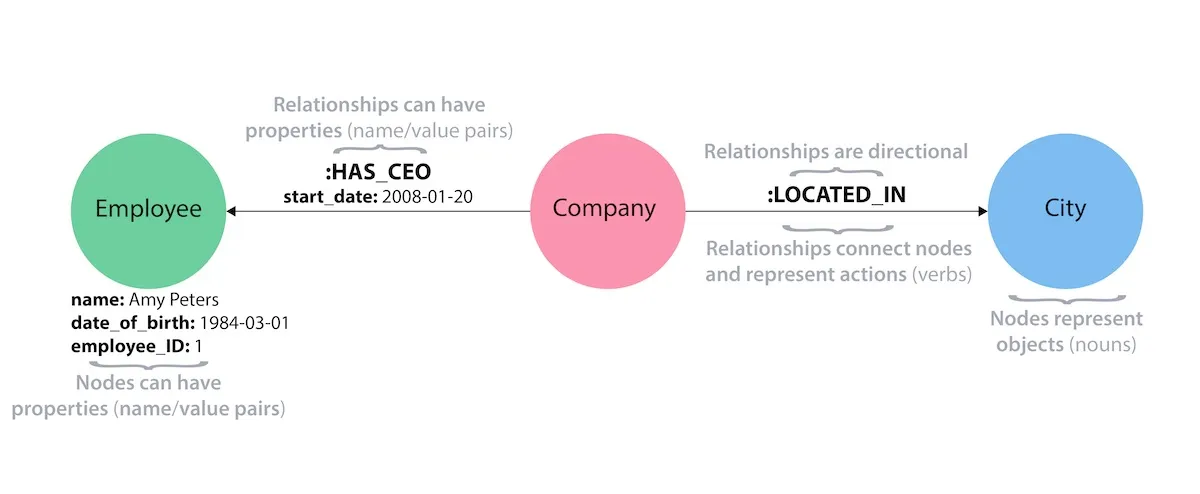
\includegraphics[width=10cm]{./Pictures/Property.png}}
      \caption{Property ของ Graph Model}\label{fig:Graph}
      \end{figure}

\newpage
      
Nodes เป็นเหมือน entity ของ Graph สามารถที่จะเก็บ attribute จำนวนมากได้ สำหรับ Graph เราจะเรียก attribute ว่า properties
Relationships เป็นความสัมพันธ์ที่เชื่อมระหว่าง 2 node และเหมือนกับ node มันสามารถเก็บ properties ได้ \\

\subsubsection {Graph Database vs Relational Database \cite{DatabaseCompare}} 

\begin{table}[!h]
  \begin{tabular}{|c|c|c|}
  \hline
  \rowcolor[HTML]{6D9EEB} 
   &
    {\color[HTML]{242424} Relational Database} &
    \cellcolor[HTML]{93C47D}{\color[HTML]{242424} Graph Database} \\ \hline
  \cellcolor[HTML]{FFFFFF}{\color[HTML]{242424} รูปแบบการเก็บข้อมูล} &
    \cellcolor[HTML]{FFFFFF}{\color[HTML]{242424} ตารางที่มีแถวและคอลัมน์} &
    {\color[HTML]{242424} \begin{tabular}[c]{@{}c@{}}โหนดที่เชื่อมต่อถึงกันพร้อมข้อมูล\\ ที่แสดงเป็นเอกสาร JSON\end{tabular}} \\ \hline
  \cellcolor[HTML]{FFFFFF}{\color[HTML]{242424} การทำงาน} &
    {\color[HTML]{242424} \begin{tabular}[c]{@{}c@{}}การทำงานของ SQL เช่น สร้าง อ่าน \\ อัปเดต และลบ (CRUD)\end{tabular}} &
    {\color[HTML]{242424} \begin{tabular}[c]{@{}c@{}}การดำเนินการรวมถึง CRUD \\ และการดำเนินการผ่านกราฟ\\ ตามทฤษฎีกราฟทางคณิตศาสตร์\end{tabular}} \\ \hline
  \cellcolor[HTML]{FFFFFF}{\color[HTML]{242424} \begin{tabular}[c]{@{}c@{}}ความสามารถ\\ ในการปรับขนาด\end{tabular}} &
    {\color[HTML]{242424} \begin{tabular}[c]{@{}c@{}}ฐานข้อมูลแบบเชิงสัมพันธ์แบบดั้งเดิม\\ สามารถปรับขนาดในแนวตั้งได้\\ แต่ไม่ค่อยเชี่ยวชาญกับการปรับขนาดในแนวนอน\end{tabular}} &
    {\color[HTML]{242424} \begin{tabular}[c]{@{}c@{}}ฐานข้อมูลแบบกราฟเชี่ยวชาญ\\ ในการปรับขนาดตามแนวนอน \\ สามารถใช้การแบ่งพาร์ติชันเพื่อกระจาย\\ ข้อมูลไปยังโหนดจำนวนมาก\end{tabular}} \\ \hline
  {\color[HTML]{242424} ประสิทธิภาพ} &
    {\color[HTML]{242424} \begin{tabular}[c]{@{}c@{}}ฐานข้อมูลแบบเชิงสัมพันธ์เผชิญกับ\\ การสืบค้นที่ซับซ้อนเมื่อสำรวจความสัมพันธ์ที่อาจ\\ ทำให้ประสิทธิภาพการทำงานช้าลง\end{tabular}} &
    {\color[HTML]{242424} \begin{tabular}[c]{@{}c@{}}ฐานข้อมูลแบบกราฟเชี่ยวชาญในการแสดง\\ และสืบค้นความสัมพันธ์ระหว่างข้อมูล\end{tabular}} \\ \hline
  {\color[HTML]{242424} \begin{tabular}[c]{@{}c@{}}ความสะดวก\\ ในการใช้งาน\end{tabular}} &
    {\color[HTML]{242424} \begin{tabular}[c]{@{}c@{}}ฐานข้อมูลแบบเชิงสัมพันธ์ทำงานได้ดีกับ\\ ชุดข้อมูลขนาดใหญ่และข้อมูลที่มีโครงสร้าง \\ พวกมันไม่ค่อยเชี่ยวชาญเมื่อเป็นเรื่อง\\ การสืบค้นแบบหลายช่วง\end{tabular}} &
    {\color[HTML]{242424} \begin{tabular}[c]{@{}c@{}}ฐานข้อมูลแบบกราฟใช้งานง่าย\\ เมื่อต้องจัดการกับข้อมูลที่เน้นความสัมพันธ์เป็นหลัก \\ เมื่อใช้ภาษาสืบค้นแบบกราฟ \\ คุณสามารถสืบค้นข้อมูลฮอป\\ หลายรายการได้อย่างรวดเร็ว\end{tabular}} \\ \hline
  \end{tabular}
  \caption{\centering Graph Database vs Relational Database}\label{tab:Graph Database vs Relational Database}
  \end{table}

\newpage

\subsection{แผนภาพ UML} 
\subsubsection{UML Diagram คืออะไร}
แผนภาพ UML \cite{UML} (UML Diagram) คือ แผนภาพที่ใช้ในการแสดงและอธิบายโครงสร้างและพฤติกรรมของ code เพื่อสื่อสารให้นักพัฒนาและผู้ที่เกี่ยวข้องทุกคนเข้าใจตรงกัน ซึ่งสามารถเอามาใช้อธิบายความสัมพันธ์ของสิ่งต่าง ๆที่อยู่ในชิ้นงานได้ โดยแผนภาพ UML มีแผนภาพหลายรูปแบบสำหรับใช้อธิบายโครงสร้างและความสัมพันธ์ในรูปแบบต่าง ๆ ที่นักพัฒนาต้องทำความเข้าใจเพื่อใช้ในการปฏิบัติงาน
\subsubsection{Use case Diagram}
Use Case Diagram เป็นหนึ่งในแผนภาพ UML ที่ใช้ในการแสดงภาพรวมของวิธีการใช้ระบบหรือซอฟต์แวร์ จากมุมมองของผู้ใช้หรือแต่ละกลุ่มผู้ใช้ โดยทำให้ง่ายต่อการเข้าใจและสื่อสารความต้องการของระบบกับผู้ใช้และทีมพัฒนา
ลักษณะหลักของ Use Case Diagram ประกอบด้วย
\begin{enumerate}
  \item Actor : แสดงตัวบุคคลหรือระบบที่มีส่วนร่วมในการใช้งานระบบ สามารถเป็นบุคคล, ระบบภายนอก, หรือภายในระบบได้
  \item Use Case : แสดงกิจกรรมหรือฟังก์ชันที่ระบบหรือซอฟต์แวร์ให้บริการในแต่ละคำสั่งหรือเหตุการณ์ที่มีผู้ใช้ร้องขอ
  \item Association : แสดงความสัมพันธ์ระหว่างผู้เกี่ยวข้องกับ Use Case
  \item System Boundary : แสดงขอบเขตของระบบที่กำหนดไว้ใน Use Case Diagram
  \item Include Relationship : แสดงว่า Use Case หนึ่งสามารถเรียกใช้ (include) Use Case อื่น ๆ ในทำนองของการนำเข้า (include)
  \item Extend Relationship : แสดงว่า Use Case นึงสามารถขยาย (extend) ไปยัง Use Case อื่น ๆ ในกรณีที่มีเหตุการณ์เฉพาะที่เกิดขึ้น
\end{enumerate}
  Use Case Diagram มีประโยชน์มากในการทำความเข้าใจและกำหนดความต้องการของระบบจากมุมมองของผู้ใช้ และช่วยให้ทีมพัฒนามีภาพรวมของฟังก์ชันและการทำงานของระบบที่ชัดเจน
\subsubsection{Sequence Diagram}
  Sequence Diagram เป็นหนึ่งในแผนภาพ UML ที่ใช้งานเพื่อแสดงลำดับขั้นตอนหรือการทำงานของวัตถุต่าง ๆ ภายในระบบหรือโปรแกรม ในแต่ละขั้นตอนของการทำงานนั้น ๆ
  ลักษณะหลักของ Sequence Diagram ประกอบด้วย

    \begin{enumerate}
      \item Lifeline : แสดงสิ่งต่าง ๆ ที่มีบทบาทในกระบวนการ สามารถเป็นวัตถุ, คลาส, หรือนักพัฒนา
      \item Message : แสดงการสื่อสารระหว่าง Lifeline สามารถแบ่งเป็น Synchronous (ทำงานพร้อมกัน) หรือ Asynchronous (ทำงานไม่พร้อมกัน)
      \item Activation Box : แสดงช่วงเวลาที่วัตถุทำงาน หรือทำการเรียกใช้งาน
      \item Return Message : แสดงการส่งคืนจากการทำงานหรือเรียกใช้งาน
      \item Focus of Control : แสดงว่าในขณะที่โปรแกรมทำงาน, ควบคุมอยู่ที่วัตถุหรือเส้นชีวิตใด
    \end{enumerate}

\subsection{Principle Design}
  \subsubsection {Principle Design คืออะไร}
  Principle Design \cite{PrincipleDesign} คือหลักการในการออกแบบที่ช่วยให้เข้าใจธรรมชาติในการรับรู้ข้อมูลและจำแนกประเภทของสมองมนุษย์ ยกตัวอย่างง่าย ๆ เช่นการที่เรานำสิ่งของที่หน้าตาคล้าย ๆ กันนำมาวางไว้ใกล้กัน

  \newpage

\subsubsection {C.R.A.P. Principle Design}
  โดยหลัก Principle design แบ่งเป็น 4 ข้อสำคัญคือ Contrast, Repetition, Alignment และ Proximity หรือตัวย่อ คือ C.R.A.P.
  \begin{enumerate}
    \item ความแตกต่าง (Contrast ) \\
    คือการแบ่งยกข้อมูลด้วยความแตกต่าง โดยความแตกต่างในที่นี้ไม่ใช่แค่สีเพียงอย่างเดียว แต่รวมถึง ขนาดที่แตกต่างกัน รูปทรงที่แตกต่างกัน เป็นต้น เมื่อใช้ความแตกต่างในการแบ่งแยกข้อมูลแล้ว จะส่งผลต่อลำดับความสำคัญในการอ่าน ทำให้เราเลือกได้ว่าจะให้ผู้ใช้งานเห็นสิ่งไหนเป็นอย่างแรก และเห็นสิ่งไหนเป็นอย่างถัดมา ซึ่งเราสามารถดูวิธีแสดงความแตกต่างตามรูปที่ \ref{fig:contrast}
    
    \begin{figure}[!h]\centering
      \setlength{\fboxrule}{0.5mm} % can define this in the preamble
      \setlength{\fboxsep}{0.5cm}
      \fbox{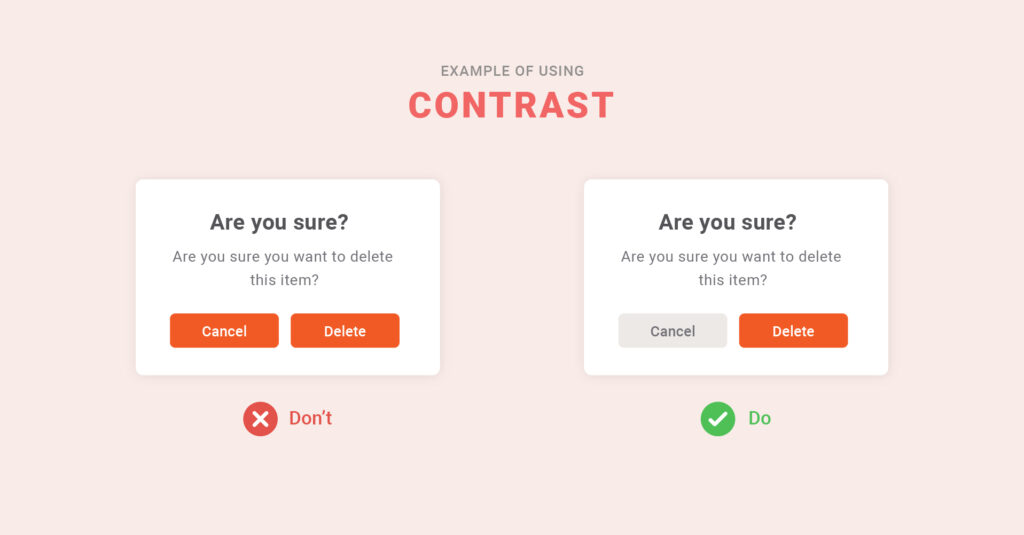
\includegraphics[width=10cm]{./Pictures/contrast.png}}
      \caption{contrast \cite{Contrast}}\label{fig:contrast}
    \end{figure}

    \item การทำซ้ำ (Repetition)\\
    การทำซ้ำในที่นี้คือการทำซ้ำของเนื้อหา ทำให้ผู้ใช้งานไม่ต้องเรียนรู้ใหม่เมื่อเจอรูปแบบการจัดวางที่คล้าย ๆ กัน ก็จะเข้าใจได้ว่ามันมีการใช้งานที่เหมือนกัน หรือจะนำ Repetition มาใช้ในการแบ่งกลุ่ม เช่นของที่มีหน้าตาเหมือนกัน เมื่อนำมาเรียงไว้ด้วยกัน ผู้ใช้จะเข้าใจได้ว่ามันคือหมวดหมู่เดียวกัน ซึ่งสามารถดูตัวอย่างการททำซ้ำได้ดังรูปที่ \ref{fig:repietition}
    
    \begin{figure}[!h]\centering
      \setlength{\fboxrule}{0.5mm} % can define this in the preamble
      \setlength{\fboxsep}{0.5cm}
      \fbox{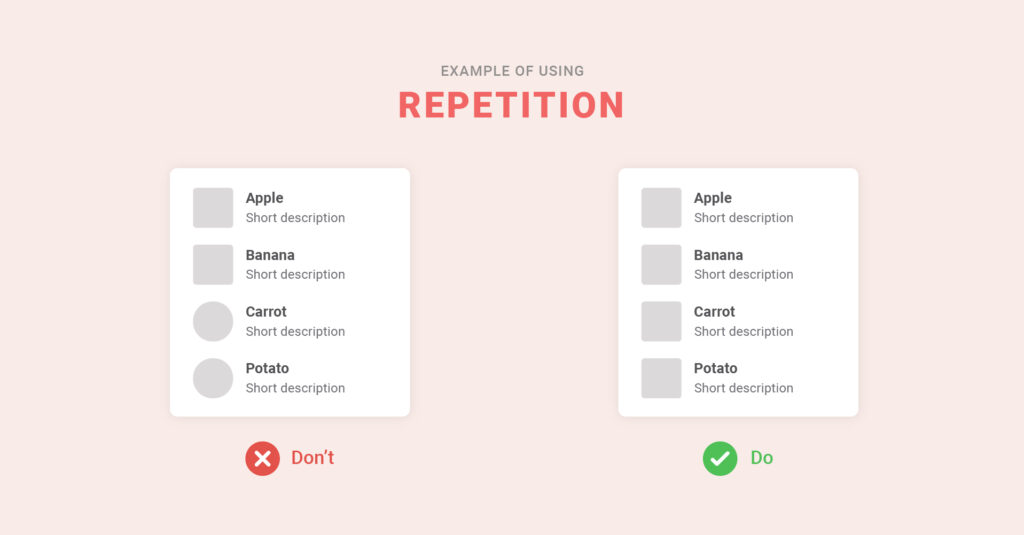
\includegraphics[width=10cm]{./Pictures/repetition.png}}
      \caption{repetition \cite{Repetition}}\label{fig:repietition}
    \end{figure}

    \newpage

    \item ตำแหน่งการจัดวาง (Alignment)\\
    ส่งผลต่อความเป็นระเบียบ ความสบายตา และความเชื่อมโยงกันของเนื้อหาโดย Alignment จะเป็น สิ่งแรก ๆ ที่ผู้ใช้งานรู้สึกได้ เมื่อมีการเปลี่ยนแปลง เมื่อจัดวางเนื้อหาในระนาบเดียวกัน ผู้ใช้จะเข้าใจได้ว่าเนื้อหานี้มีความเชื่อมโยงกัน ซึ่งสามารถดูตัวอย่างการจัดวางได้ตามรูปที่ \ref{fig:alignment}
    
    \begin{figure}[!h]\centering
      \setlength{\fboxrule}{0.5mm} % can define this in the preamble
      \setlength{\fboxsep}{0.5cm}
      \fbox{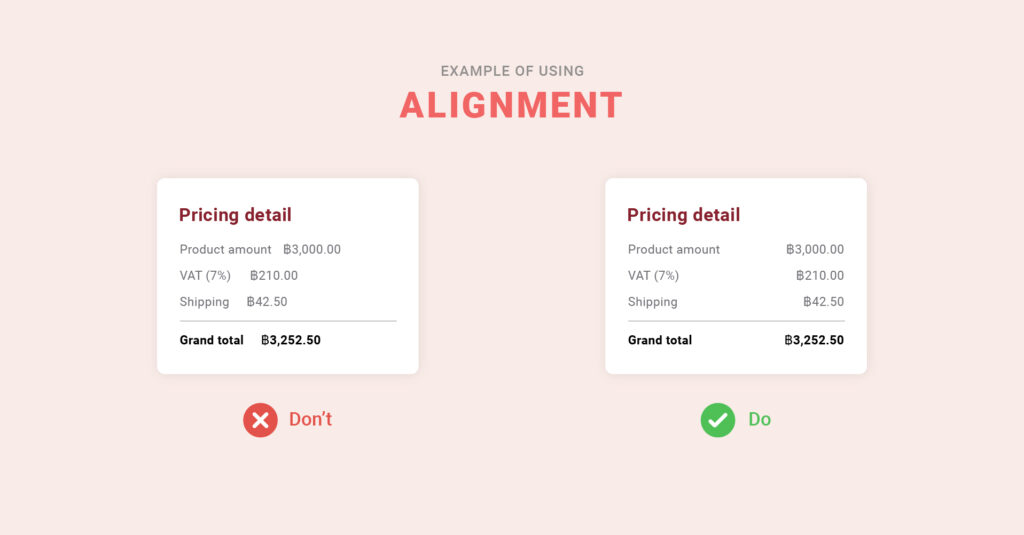
\includegraphics[width=10cm]{./Pictures/alignment.png}}
      \caption{alignment \cite{Alignment}}\label{fig:alignment}
    \end{figure}

    \item การจัดกลุ่มข้อมูล (Proximity) \\
    คือการจัดวางองค์ประกอบของข้อมูล โดยข้อมูลที่มีความเชื่อมโยงกันควรจัดให้เป็นกลุ่มก้อนเดียวกัน จะช่วยให้ข้อมูลในหน้าเว็บไซต์ หรือแอปพลิเคชั่นที่เราออกแบบมีความซับซ้อนน้อยลง และมีการแบ่งหมวดหมู่ชัดเจนขึ้น ซึ่งจะเห็นได้ดังตัวอย่างในรูปที่ \ref{fig:proximity}
    
    \begin{figure}[!h]\centering
      \setlength{\fboxrule}{0.5mm} % can define this in the preamble
      \setlength{\fboxsep}{0.5cm}
      \fbox{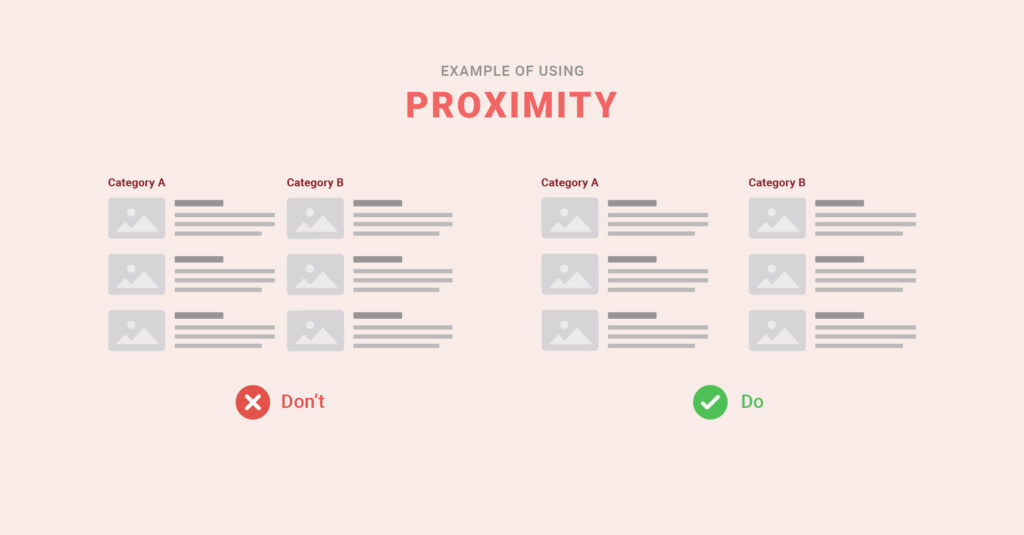
\includegraphics[width=10cm]{./Pictures/proximity.png}}
      \caption{proximity \cite{Proximity}}\label{fig:proximity}
    \end{figure}
  \end{enumerate}

\newpage

\section{เทคโนโลยี}
  \subsection{Integrated Development Environment (IDE)}

    \begin{itemize}
      \item Visual Studio Code \cite{VSCode} \\ 
        โปรแกรมสำหรับเขียนโค้ดที่ใช้ในการแก้ไขและปรับแต่งโค้ด จากค่ายไมโครซอฟท์ มีการพัฒนาออกมาในรูปแบบของ OpenSource จึงสามารถนำมาใช้งานได้แบบฟรี ๆ สนับสนุนภาษาโปรแกรมมิ่งมากมายทั้งภาษา JavaScript, TypeScript และ Node.js สามารถเชื่อมต่อกับ Git ได้ นำมาใช้งานได้ง่ายไม่ซับซ้อน มีเครื่องมือส่วนขยายต่าง ๆ ให้เลือกใช้อย่างมากมาย
      \item Pycharm \cite{Pycharm} \\ 
        โปรแกรมสำหรับเขียนโค้ดสำหรับภาษาไพทอน ติดตั้งบนเครื่องคอมพิวเตอร์ ได้ทั้งบนระบบปฏิบัติการ Windows, MacOS และ Linux 
      \item Google Colab \cite{Colab} \\ 
        โปรแกรมสำหรับเขียนโค้ดสำหรับภาษาไพทอนในเบราว์เซอร์ โดยไม่ต้องกำหนดค่าใดและสามารถเข้าถึง GPU โดยไม่มีค่าใช้จ่าย
    \end{itemize}

  \subsection{Design}
    \begin{itemize}
      \item Figma \cite{Figma} \\ 
        เครื่องมือออกแบบ User interface โดยสามารถใช้ออกแบบได้ตั้งแต่เว็บไซต์ แอปพลิเคชัน หรือโลโก้ ในรูปแบบที่มีลูกเล่นมากกว่าที่เคยเห็นในอดีต เช่น การออกแบบ Interactive component เป็นต้น
      \item LucidChart \cite{Lucidchart} \\ 
        เว็บแอปพลิเคชันสำหรับสร้างไดอะแกรม ผังงาน แผนภาพแบบจำลอง หรือแผนที่ความคิด สามารถแชร์แผนภาพให้ผู้อื่นเพื่อทำงานร่วมกันแบบเรียลไทม์ได้ มีเทมเพลตสำเร็จรูปให้เลือกใช้งานได้หลากหลายรูปแบบ เช่น ผังงาน แบบโครงร่าง แผนภาพเครือข่าย และแผนผังเว็บไซต์ เป็นต้น นอกจากนี้ยังสามารถแสดงความคิดเห็น หรือสนทนาแบบกลุ่มได้ และยังดาวน์โหลดเป็นไฟล์รูปแบบต่าง ๆ ได้
    \end{itemize}

  \subsection{Frontend}
    \begin{itemize}
      \item React Native \cite{ReactNative} \\ 
        Cross-Platform Framework ที่ใช้ในการพัฒนา Native Mobile Application สำหรับ Android และ iOS ที่พัฒนาโดยบริษัท Facebook Inc. 
        React Native มีหลักการคล้ายกับ Xamarin คือสามารถ Reuse Code ได้มากกว่า 70% ในการทำแอปพลิเคชันที่รันได้ทั้งบน Android และ iOS โดยใช้ภาษาหลักคือภาษา Javascript และ Typescript ในการพัฒนาแอปพลิเคชัน ซึ่งเมื่อทำเสร็จแอปพลิเคชันจะทำงานไวใกล้เคียงกับการเขียนด้วย ภาษา Native อย่าง Java และ Swift/Objective-C อีกหนึ่งจุดเด่นของ React Native คือการประยุกต์ใช้แนวคิดแบบ Reactive Programming ที่ทำให้การพัฒนารองรับการทำงานแบบ Asynchronous และมี State ที่ซับซ้อนได้
    \end{itemize}

  \subsection{Backend}
    \begin{itemize}
      \item FastAPI \cite{FastAPI} \\ 
        FastAPI คือเว็บเฟรมเวิร์กที่มีความรวดเร็วและประสิทธิภาพสูง สำหรับการสร้าง API ด้วยภาษา Python ที่มีจุดเด่นได้แก่
        \begin{enumerate}
          \item มีความรวดเร็ว ประสิทธิภาพเทียบเท่ากับ NodeJS และ Go 
          \item สร้างง่าย เพิ่มความเร็วในการพัฒนา
          \item ลดข้อผิดพลาดที่เกิดจากมนุษย์ (นักพัฒนา)
        \end{enumerate}
    \end{itemize}

  \subsection{Database}
    \begin{itemize}
      \item Neo4j \cite{Neo4j} \\ 
        เป็นระบบฐานข้อมูลที่ถูกออกแบบมาเพื่อจัดเก็บข้อมูลแบบกราฟ (Graph Database) ที่สามารถจัดเก็บแมปและสอบถามความสัมพันธ์ระหว่างข้อมูลได้อย่างมีประสิทธิภาพและมีความยืดหยุ่น ระบบฐานข้อมูลกราฟนี้ถูกออกแบบมาเพื่อเก็บข้อมูลในรูปแบบของ Node และ เชื่อมต่อระหว่างโหนดด้วยเส้นเชื่อมที่เรียกว่า Relationships ทำให้สามารถแสดงความสัมพันธ์และการเชื่อมโยงของข้อมูลได้อย่างชัดเจน
    \end{itemize}

  \subsection{Machine Learning}
    \begin{itemize}
      \item mT5 \\
        เป็นโมเดลการเรียนรู้ของเครื่องสำหรับการประมวลภาษาธรรมชาติที่มีความหลากหลายในการรับรองภาษาต่าง  ๆ ซึ่งถูกพัฒนาโดย Google Research และเป็นการปรับปรุงจากโมเดล T5 (Text-to-Text Transfer Transformer) ซึ่งเป็นโมเดลที่มีความสามารถในการเรียนรู้จากข้อมูลข้อความและการประมวลผลข้อความอย่างมีประสิทธิภาพ
      \item BERT-th  \\
        เป็นโมเดลการเรียนรู้ของเครื่องสำหรับการประมวลภาษาธรรมชาติที่ถูกพัฒนาขึ้นเพื่อใช้ในภาษาไทย โมเดลนี้มีความสามารถในการเข้าใจและประมวลผลข้อมูลที่เป็นภาษาไทยอย่างมีประสิทธิภาพ โดยใช้หลักการของ BERT (Bidirectional Encoder Representations from Transformers) ซึ่งเป็นโมเดลการเรียนรู้ของเครื่องที่สามารถทำนายคำถัดไปในประโยคจากข้อมูลทั้งด้านซ้ายและด้านขวาของคำนั้น ๆ
      \item fastText \\
        เป็น library สำหรับการทำโมเดลการเรียนรู้ของเครื่องสำหรับการประมวลภาษาธรรมชาติ พัฒนาโดย Facebook AI Research และเน้นการสร้างเวกเตอร์คำและการจัดกลุ่มคำศัพท์ โดยใช้หลักการของการแปลงคำเป็นเวกเตอร์ที่สามารถใช้ในการค้นหาความคล้ายคลึงระหว่างคำ
      \item thai2fit \\
        เป็นโมเดลการเรียนรู้ของเครื่องสำหรับการประมวลภาษาธรรมชาติที่ได้รับการปรับปรุงและเพิ่มประสิทธิภาพสำหรับการทำงานกับข้อมูลภาษาไทย โดยใช้หลักการของ fastText และ Word Embedding ที่ถูกพัฒนามาเพื่อภาษาไทย 
      \item BERT-Base-Multilingual-Case \\
        เป็นโมเดลการเรียนรู้ของเครื่องสำหรับการประมวลภาษาธรรมชาติที่รองรับหลายภาษาและมีความสามารถในการประมวลผลข้อความในหลายภาษาที่มีตัวอักษรต่างกัน โมเดลนี้ถูกพัฒนาโดย Google และเป็นการปรับปรุงจาก BERT โดยรองรับการแปลงตัวอักษรเป็นตัวพิมพ์ใหญ่และตัวพิมพ์เล็ก
      \item Thai nlp \\
        เป็นแหล่งข้อมูลหลักสำหรับนักวิจัยและผู้พัฒนาที่กำลังทำงานด้าน Natural language processing ในภาษาไทย ซึ่งจะรวบรวมเครื่องมือการทำ Natural language processing  โมเดลที่พร้อมใช้งานและ ข้อมูลที่เป็นประโยชน์สำหรับงานวิจัยและการพัฒนาในด้าน NLP ในภาษาไทยเอาไว้ โดยมีความหลากหลายของเครื่องมือและข้อมูลที่มีคุณภาพสูง เช่น โมเดลการแปลภาษา การจัดกลุ่มคำศัพท์ และวิธีการประมวลผลข้อมู ที่ถูกพัฒนาให้ใช้งานได้อย่างมีประสิทธิภาพ
    \end{itemize}

  \subsection{Version Control}
    \begin{itemize}
      \item Git \cite{Git} \\
        Version Control ตัวหนึ่งซึ่งจะเป็นระบบที่มีหน้าที่ทำการจัดเก็บการเปลี่ยนแปลงของไฟล์ใน Project และมีการ backup ให้สามารถที่จะเรียกดูหรือทำการย้อนกลับไปดูเวอร์ชั่นต่าง ๆ ของ Project ที่ใด เวลาใดก็ได้ ดังนั้น Version Control ก็เหมาะอย่างยิ่งสำหรับนักพัฒนาไม่ว่าจะเป็นทั้งในรูปเเบบเดี่ยวหรือกลุ่มก็ตาม และนอกจากนั้นก็ยังสามารถเรียกดูได้ ว่าใครเป็นคนเขียนหรือใครเป็นคนแก้ไข Project ในส่วนต่าง
      \item Github \\
        เว็บเซิฟเวอร์ที่ให้บริการในการฝากไฟล์ Git หรือพูดง่าย ๆ ก็คือ Git ที่อยู่บนเว็บไซต์นั่นเอง ซึ่งจะทำให้สามารถใช้ Git ร่วมกับคนอื่นได้โดยผ่านเว็บไซต์ซึ่งจะมักนิยมใช้กันมาก ในการเก็บ Project Open Source ต่าง ๆ
    \end{itemize}

  \subsection{Testing}
    \begin{itemize}
      \item Jest \cite{Jest}\\
        JavaScript Framework สำหรับเอาไว้เขียน Test เป็น Open Source ที่พัฒนาโดย Facebook ซึ่งมี helper มี function ต่าง ๆ ให้ใช้ ทำให้ง่ายต่อการเขียน Test สามารถเขียนเทสได้ทั้ง React, Vue, Angular หรือ JavaScript ทั่ว ๆ ไป
      \item PyTest \\
        เป็นหนึ่งในเครื่องมือทดสอบโค้ดโปรแกรมภาษาไพทอนยอดนิยม โดย รองรับทั้ง Python 2 , Python 3 มี auto-discovery และอื่น ๆ 
        ใช้ License: MIT license
    \end{itemize}

\section{แบบสำรวจผลิตภัณฑ์}
  ModLink คือแอปพลิเคชั่นของทางมหาวิทยาลัยโดยข้อมูลภายใน แอปพลิเคชั่นนั้น จะเกี่ยวกับข้อมูลกิจกรรมต่าง ๆ ภายในมหาวิทยาลัย และข้อมูลส่วนตัวของนักศึกษา อย่างไรก็ตาม feature การแสดงข้อมูลเกี่ยวกิจกรรมของแอปพลิเคชันนี้ยังถือว่าทำได้ไม่ค่อยดีนัก เนื่องจากเป็นการกระจายข่าวสาร แบบทั่วไป ไม่ได้แบ่งแยกประเภทหรือแสดงตามที่ผู้ใช้ให้ความสนใจ ตัวอย่างหน้า UI ของ ModLink อยู่ในรูปที่ \ref{fig:modlink}

  \begin{figure}[!h]\centering
    \setlength{\fboxrule}{0.5mm} % can define this in the preamble
    \setlength{\fboxsep}{0.5cm}
    \fbox{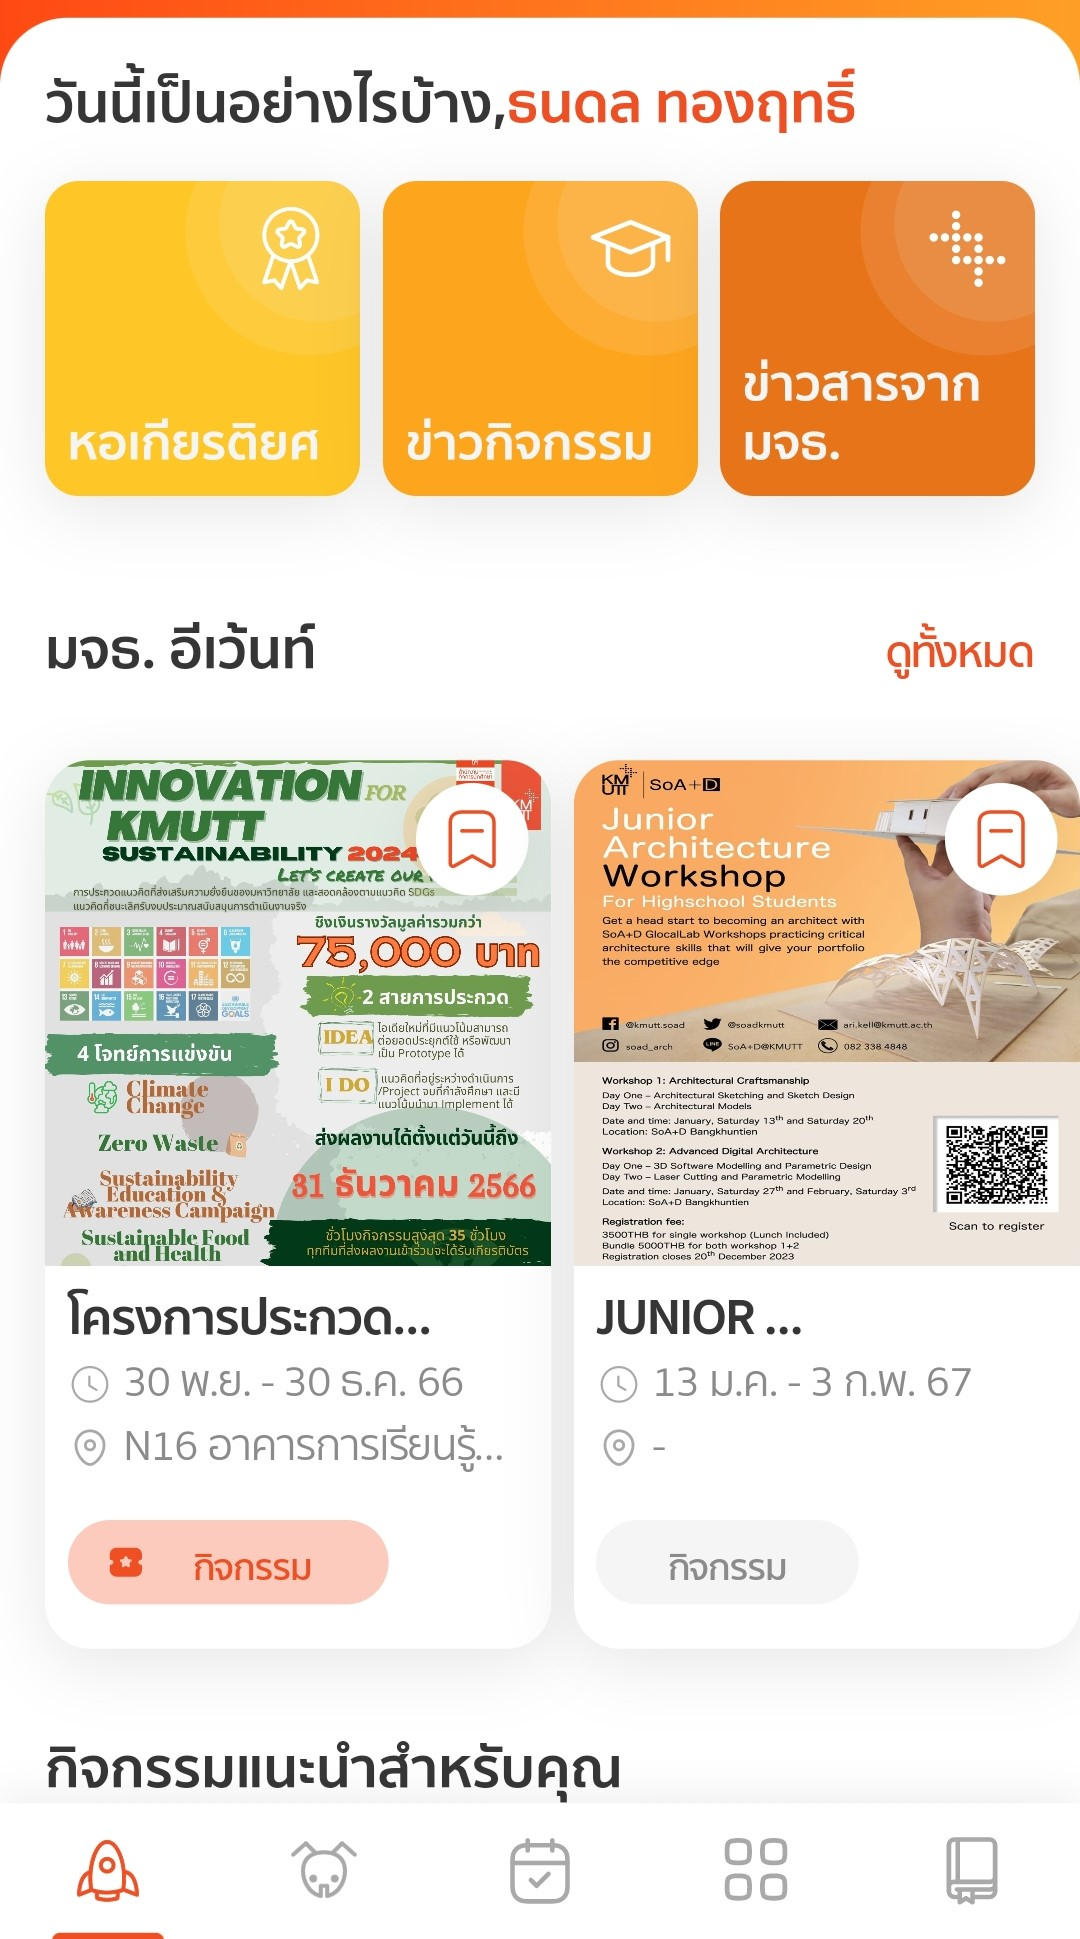
\includegraphics[width=5cm]{./Pictures/modlink.jpg}}
    \caption{หน้าแนะนำกิจกรรมของ ModLink และรายละเอียด}\label{fig:modlink}
    \end{figure}

\newpage

KMUTT Hatch คือ เว็บไซต์สำหรับนักศึกษาและศิษย์เก่าเพื่อประชาสัมพันธ์กิจกรรมของ Hatch ทางเว็บไซต์มีการประชามสัมพันธ์กิจกรรมต่าง ๆ และข้อมูลที่จำเป็นต่อผู้ใช้งาน อย่างไรก็ตามเว็บไซต์นี้สามารถประชาสัมพันธ์ได้แค่กิจกรรมที่ทาง Hatch เป็นผู้จัดเท่านั้น

  \begin{figure}[!h]\centering
    \setlength{\fboxrule}{0.5mm} % can define this in the preamble
    \setlength{\fboxsep}{0.5cm}
    \fbox{
\includegraphics[width=10cm]{./Pictures/hatch.png}}
    \caption{หน้าแนะนำกิจกรรมของ KMUTT Hatch}\label{fig:hatch}
    \end{figure}



KMUTT Sinfo คือ เว็บไซต์สำหรับนักศึกษาที่ทำการรวบรวมระบบจัดการงานต่าง ๆ ของนักศึกษาไม่ว่าจะเป็นการลงทะเบียนเรียน ดูเกรด หรือประเมินกิจกรรม ซึ่งแม้ว่างานต่าง ๆ ของนักศึกษานั้นจะมีศูนย์กลางมาที่เว็บไซต์นี้ แต่ถึงกระนั้นก็เป็นเว็บที่ใช้งานไม่ค่อยสะดวก เนื่องจากต้องเข้าผ่าน pop up ซึ่งต้องอาศัยการตั้งค่าและยังใช้งานไม่ได้ในบาง platform อีกทั้งยังจำกัดเวลาที่ใช้งานเอาไว้และแม้จะเป็นศูนย์รวมประวัติการทำกิจกรรมของนักศึกษา แต่กลับไม่สามารถแนะนำได้ว่านักศึกษานั้นให้ความสนใจในกิจกรรมใด ตัวอย่างหน้าใช้งานของ KMUTT sinfo อยู่ในรูปที่ \ref{fig:sinfo}

  \begin{figure}[!h]\centering
    \setlength{\fboxrule}{0.5mm} % can define this in the preamble
    \setlength{\fboxsep}{0.5cm}
    \fbox{
\includegraphics[width=10cm]{./Pictures/sinfo.png}}
    \caption{หน้า Mainpage ของ KMUTT Sinfo}\label{fig:sinfo}
    \end{figure}

\newpage

Padlet คือแอปพลิเคชันหรือเว็บไซต์ที่อยู่ในแพลตฟอร์มสำหรับ การระดมความคิด แสดงความคิดเห็น หรือแลกเปลี่ยนความรู้ร่วมกัน ผ่านกระดานดิจิทัลในรูปแบบเสมือน Post it ที่ติดบนบอร์ด ซึ่งจะแสดงผลทุกอย่างแบบ Real-time สามารถโพสต์ทั้งในรูปแบบข้อความ รูปภาพ และลิงก์ของเว็บไซต์ได้ เว็บเพจที่จะให้ผู้ใช้มาแสดงความเห็น หรือโพสต์ข้อมูลลงบนเว็บ ซึ่งจะต่างจากตรงที่ทางระบบของจะเป็นตัวกลางในการคำนวนหาจากความชื่นชอบของผู้ใช้จากกิจกรรมที่ผู้ใช้เคยได้เข้าร่วม หรือชมรมที่ผู้ใช้สนใจอยู่ หน้าที่เข้าไปยังบอร์ดต่าง ๆ ของ Padlet อยู่ในรูปที่ \ref{fig:padlet}

  \begin{figure}[!h]\centering
    \setlength{\fboxrule}{0.5mm} % can define this in the preamble
    \setlength{\fboxsep}{0.5cm}
    \fbox{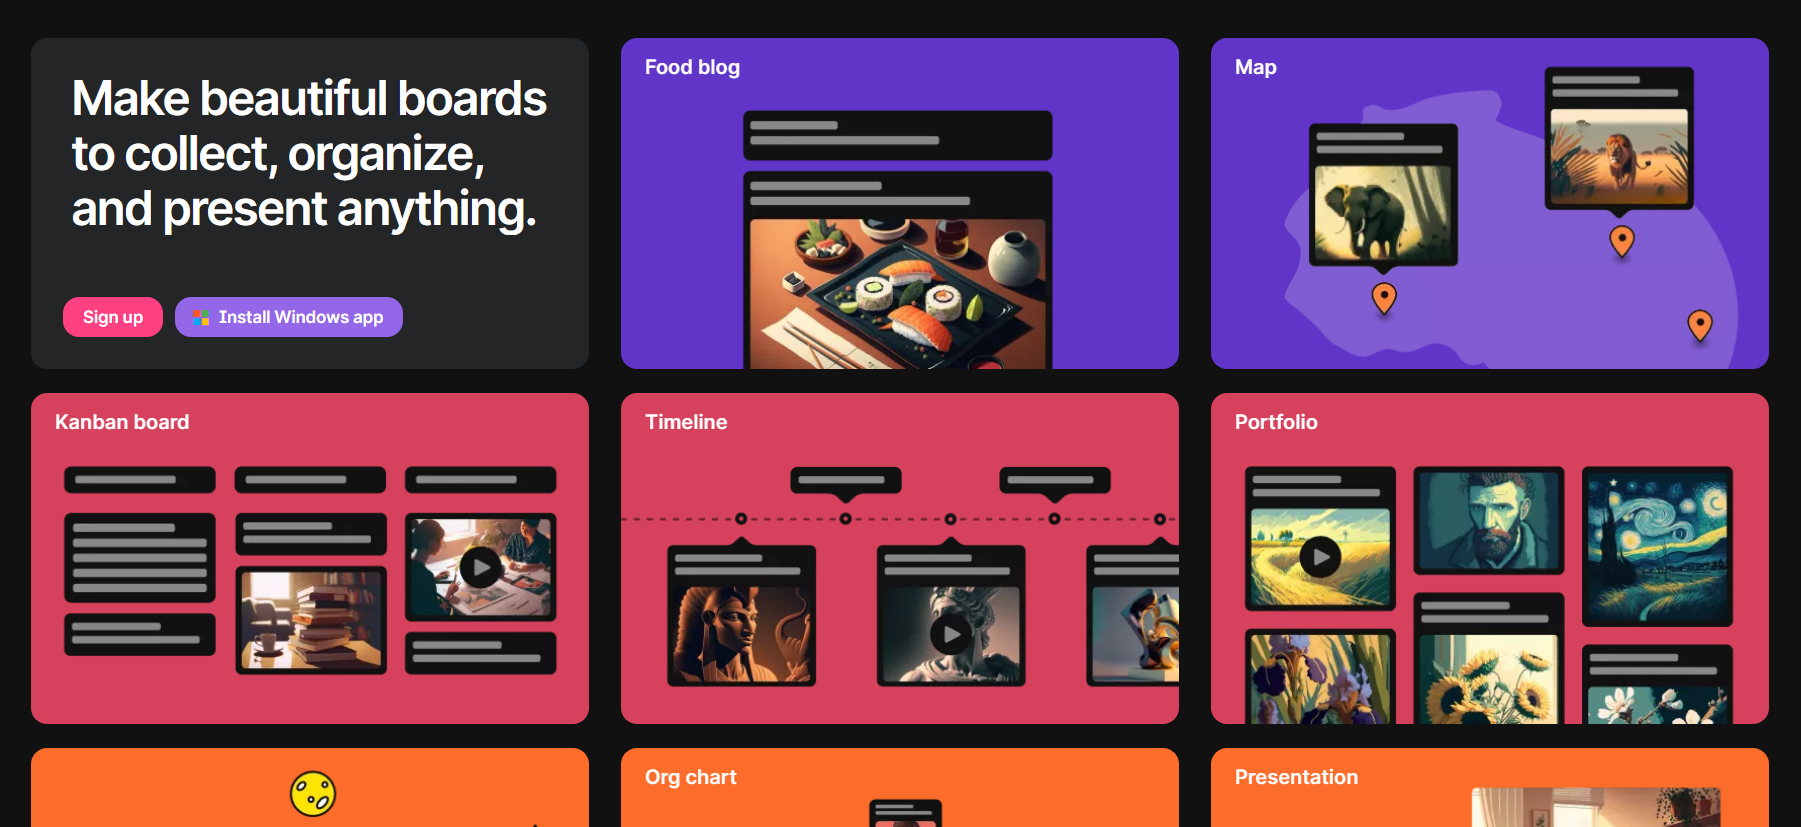
\includegraphics[width=10cm]{./Pictures/padlet.png}}
    \caption{หน้า Mainpage ของ Padlet}\label{fig:padlet}
    \end{figure}

Pantip คือ พื้นที่สำหรับการแลกเปลี่ยนความคิดเห็นในหัวข้อ หรือประเด็นที่สนใจร่วมกัน สามารถสอบถาม บอกเล่าแบ่งปันประสบการณ์ในเรื่องต่าง ๆ ในหน้ากระดานสนทนาโดยสมาชิกสามารถตั้ง หรือตอบกระทู้ต่าง ๆ ที่สมาชิกสนใจและสามารถเลือกหาอ่านข้อมูลได้จากป้ายหัวข้อในเรื่องต่าง ๆ ที่ทางเว็บไซต์ ได้สร้างขึ้นไว้ ซึ่งจะต่างจากตรงที่ทางระบบของ จะเป็นตัวกลางในการคำนวนหาจากความชื่นชอบของผู้ใช้จากกิจกรรมที่ผู้ใช้เคยได้เข้าร่วม หรือชมรมที่ผู้ใช้สนใจอยู่ โดยรูปที่ \ref{fig:pantip} คือหน้าที่แสดงเนื้อหาต่าง ๆ ของ Pantip

  \begin{figure}[!h]\centering
    \setlength{\fboxrule}{0.5mm} % can define this in the preamble
    \setlength{\fboxsep}{0.5cm}
    \fbox{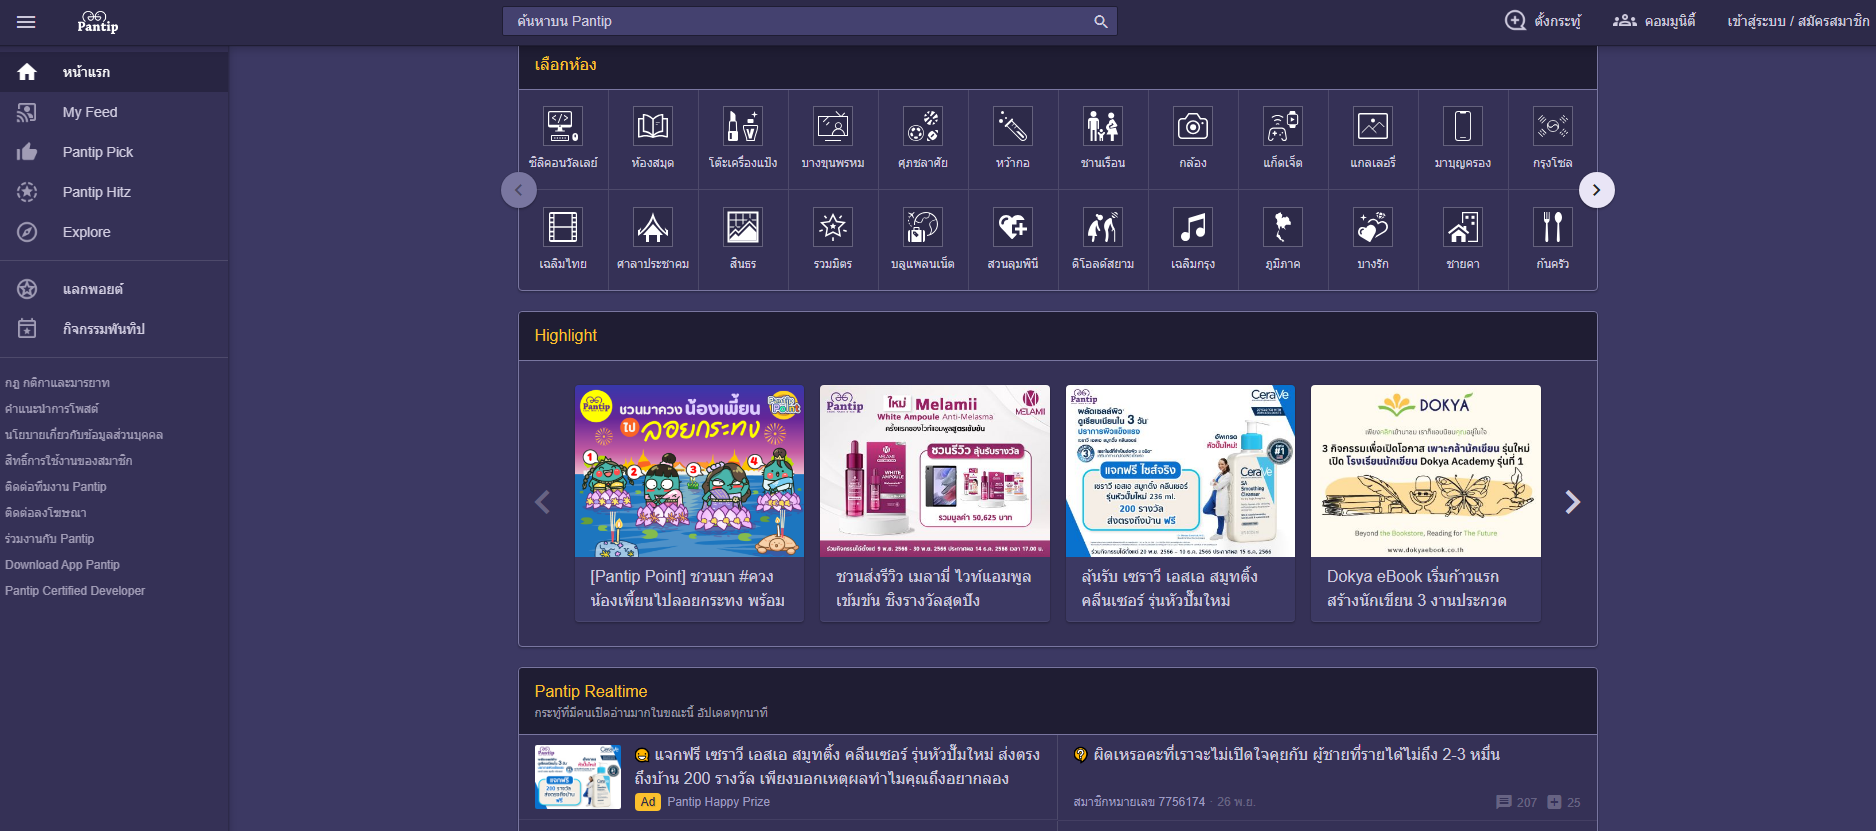
\includegraphics[width=10cm]{./Pictures/pantip.png}}
    \caption{หน้าแนะนำกระทู้ของ Pantip}\label{fig:pantip}
    \end{figure}

Facebook เป็น social media ที่ได้รับความนิยมที่สามารถใช้งาน ได้ในหลาย platform ซึ่งสามารถนำเสนอข้อมูลข่าวสารให้ผู้ใช้งานได้มากมายและเป็น social media ที่มีคนใช้งานแทบตลอดทั้งวัน ทำให้บางชมรมเลือก
ที่จะทำหน้าเพจเพื่อกระจายข่าวสารเกี่ยวกับชมรมของตัวเอง อย่างไรก็ตามด้วยปริมาณข่าวสารมากมายของ facebook ทำให้ข่าวสารของชมรมมักโดนกลบด้วย  ข่าวอื่น ๆ อยู่เสมอ ถึงแม้จะสามารถเข้าไปสู่หน้าเพจเพื่อดูความเคลื่อนไหวได้แต่ก็ไม่สามารถแนะนำตัวชมรมหรือกิจกรรมที่ชมรมจะจัดให้แก่นักศึกษาที่ไม่ติดตามเพจได้อยู่ดี โดยตัวอย่างเพจเพื่อประชาสัมพันธ์ใน Facebook ดูได้ในรูปที่ \ref{fig:facebook}

  \begin{figure}[!h]\centering
    \setlength{\fboxrule}{0.5mm} % can define this in the preamble
    \setlength{\fboxsep}{0.5cm}
    \fbox{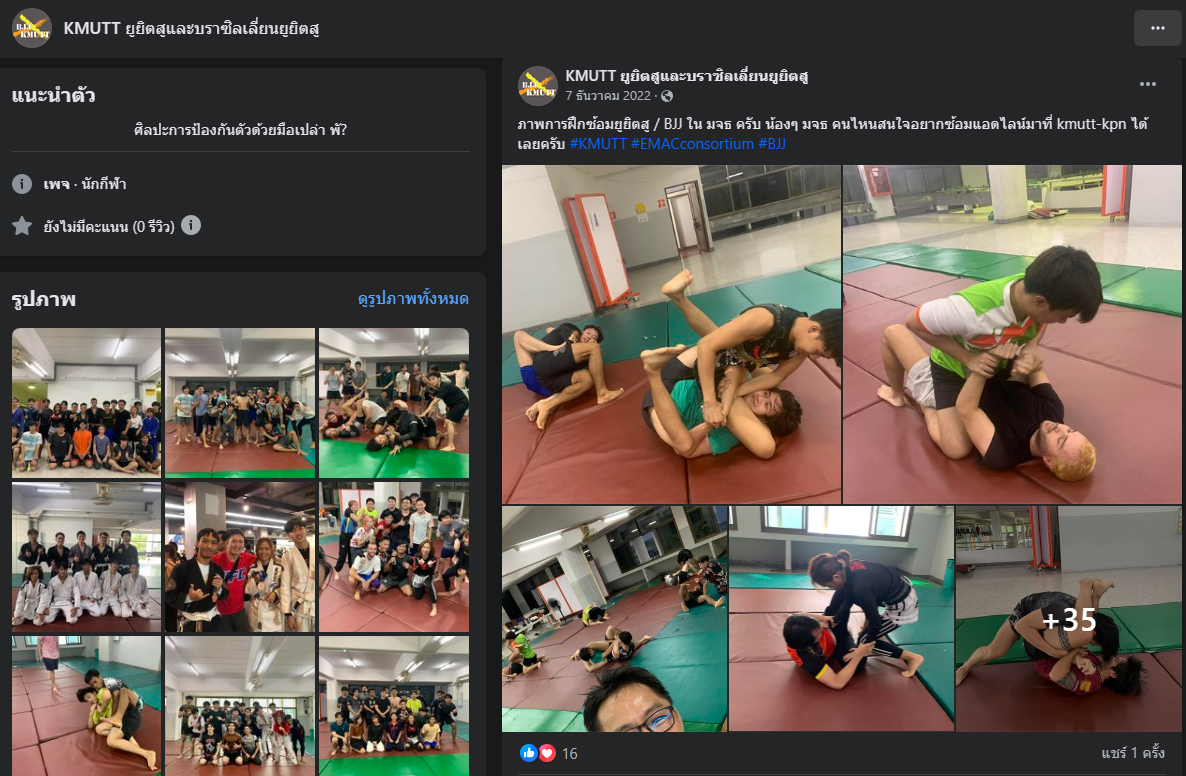
\includegraphics[width=10cm]{./Pictures/facebook.png}}
    \caption{หน้า Homepage ของเพจชมรมใน Facebook}\label{fig:facebook}
    \end{figure}

\newpage

Instagram คือ แอปพลิเคชันบน smartphone และอุปกรณ์คอมพิวเตอร์ โดยแอปพลิเคชันนี้จะเน้นการแชร์รูปภาพ บน Social Network ซึ่งทำให้เพื่อน ของคุณสามารถเห็นภาพถ่ายของคุณได้และยังสามารถคอมเมนต์ภาพของคุณได้  	   ที่สำคัญ Instagram ยังสามารถแชร์ภาพของคุณไปยัง Twitter และ Facebook ได้อีกด้วย ยังสามารถกดติดตามบุคคลที่ชื่นชอบเพื่อที่จะได้เห็นโพสต์รูปภาพ วิดีโอ ของบุคคลนั้น ๆ ได้อีกด้วย และยังมีฟีเจอร์ story ที่ใช้ในการอัพรูปภาพ วิดีโอคลิปของคุณได้ด้วย โดยตัวอย่างของ instargram ของทางชมรมสามารถดูได้จากภาพที่ \ref{fig:ig}

  \begin{figure}[!h]\centering
    \setlength{\fboxrule}{0.5mm} % can define this in the preamble
    \setlength{\fboxsep}{0.5cm}
    \fbox{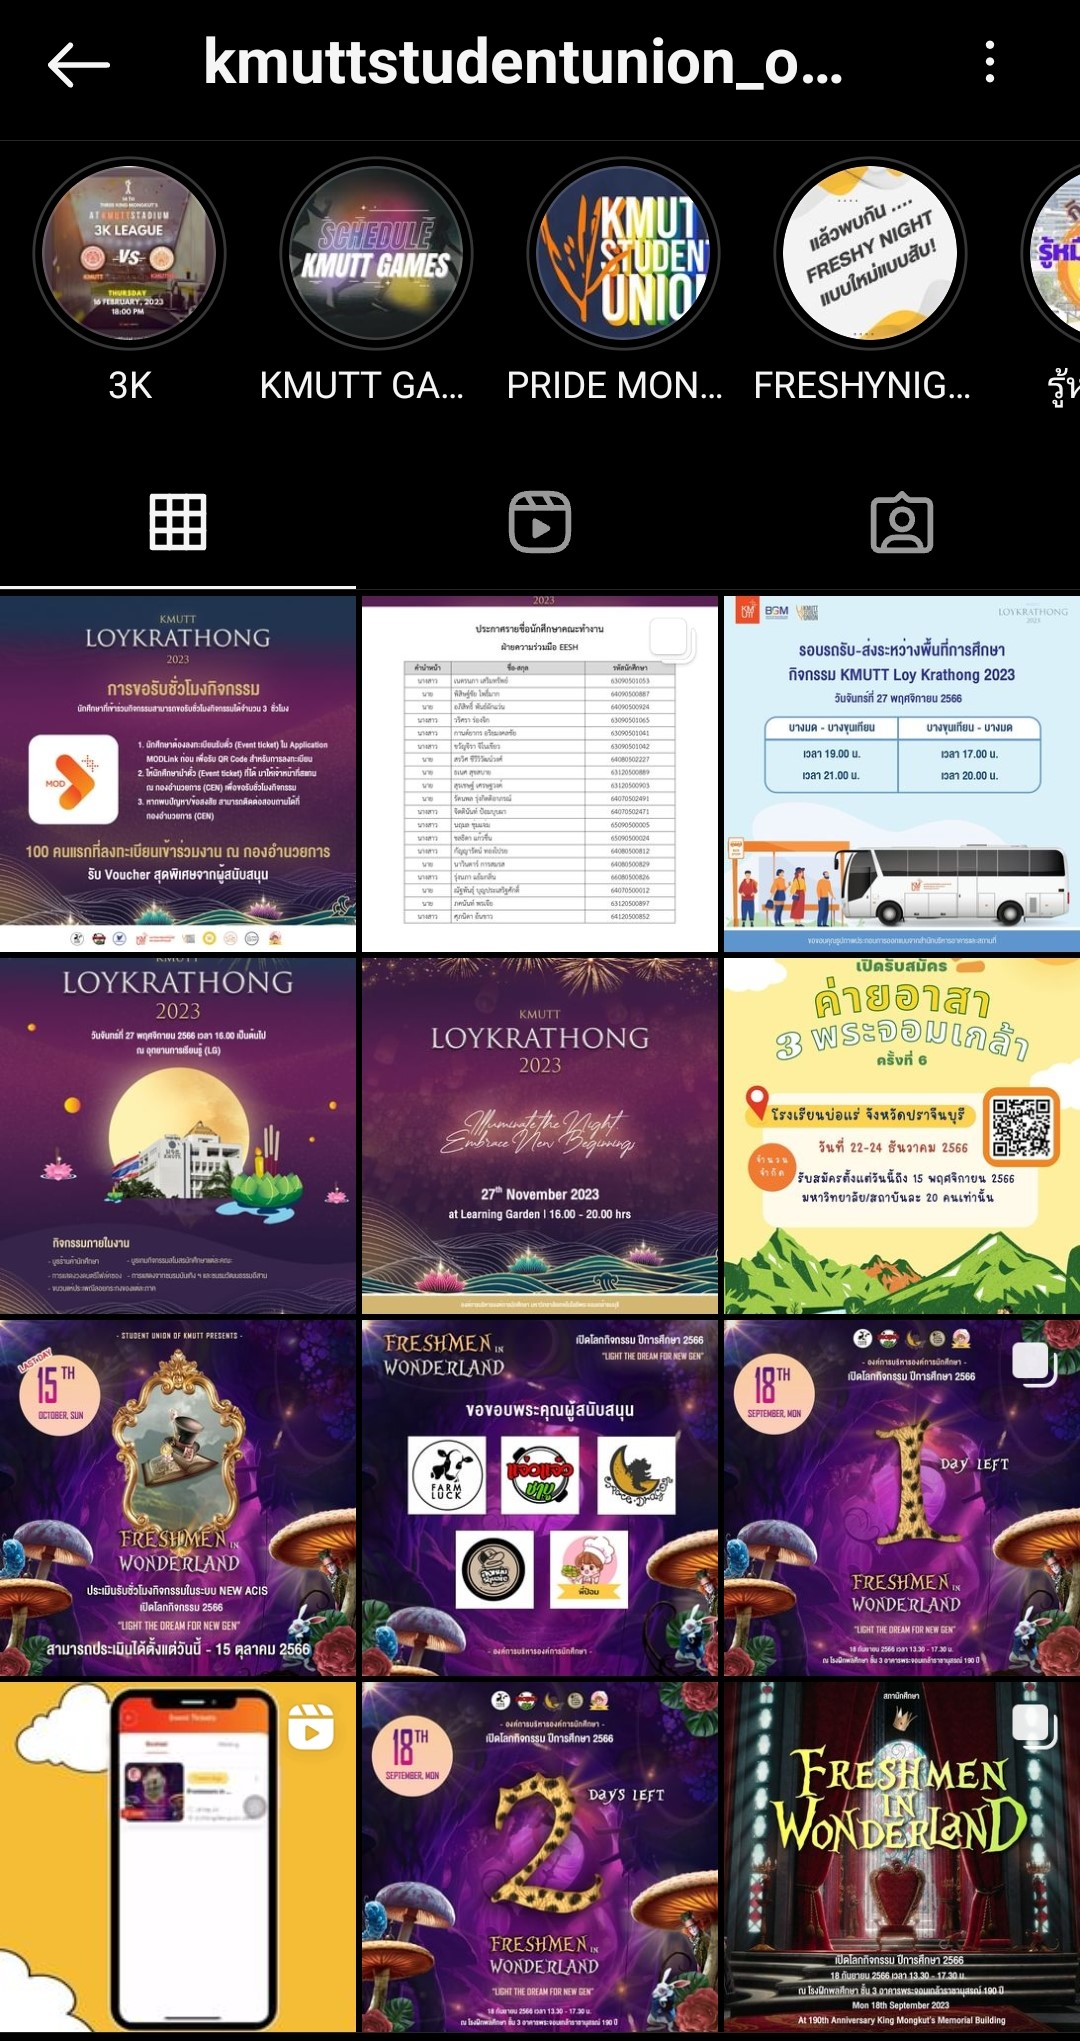
\includegraphics[width=5cm]{./Pictures/ig.jpg}}
    \caption{หน้า Notifications ของ Instargram}\label{fig:ig}
    \end{figure}

\newpage

\large\textbf{ตารางความแตกต่างของ Feature}

  \begin{figure}[!h]\centering
    \setlength{\fboxrule}{0.5mm} % can define this in the preamble
    \setlength{\fboxsep}{0.5cm}
    \fbox{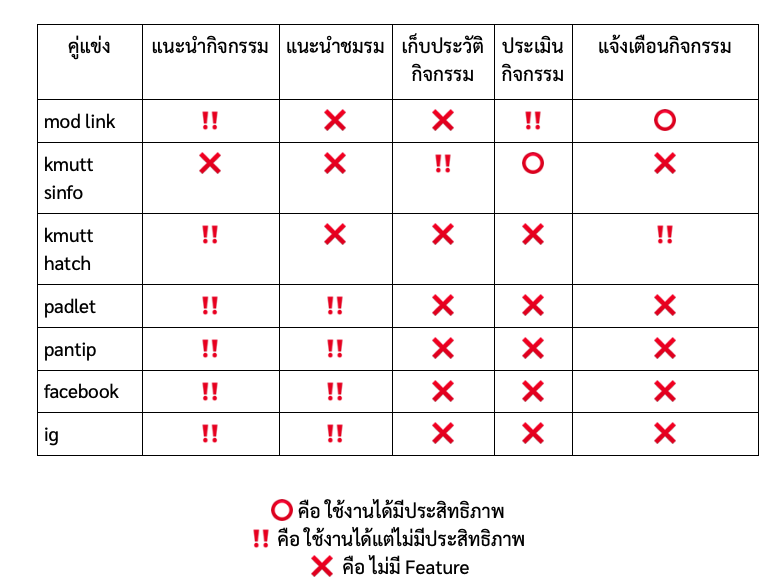
\includegraphics[width=15cm]{./Pictures/DiffFeat.png}}
    \caption{ตารางความแตกต่างของ Feature}\label{fig:DiffFeat}
    \end{figure}

\newpage

\large\textbf{ระบบการแนะนำกิจกรรม} \large

  \begin{figure}[!h]\centering
    \setlength{\fboxrule}{0.5mm} % can define this in the preamble
    \setlength{\fboxsep}{0.5cm}
    \fbox{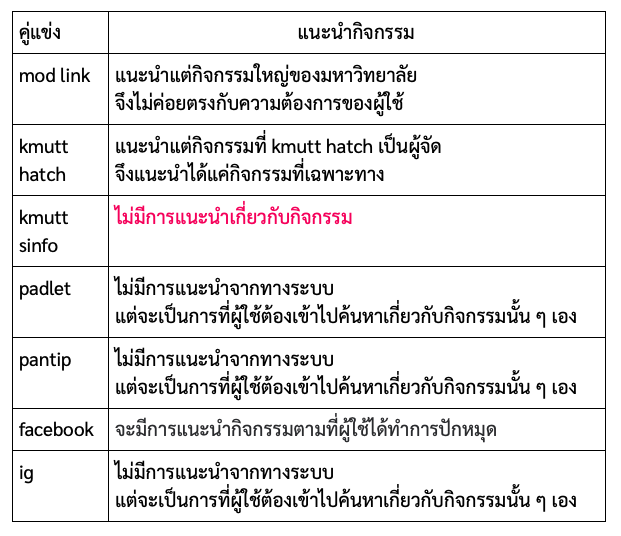
\includegraphics[width=15cm]{./Pictures/Suggest.png}}
    \caption{ระบบการแนะนำกิจกรรม}\label{fig:Suggest}
    \end{figure}

\chapter{วิธีการทำงาน กระบวนการและการออกแบบ}
ในบทนี้จะกล่าวถึงการสำรวจความต้องการของผู้ใช้งานเพื่อนำมาวิเคราะห์คุณลักษณะที่โครงการควรมี และนำสิ่งที่วิเคราะห์ได้มาใช้ออกแบบโครงสร้างและองค์ประกอบต่าง ๆ ของตัวผลิตภัณฑ์ โดยจะมีการอธิบายโครงสร้างและองค์ประกอบต่าง ๆ ที่อยู่ในตัวผลิตภัณฑ์รวมถึงวิธีการทำงานโดยละเอียด
\section{บทนำ}
\subsection{สำรวจความต้องการของผู้ใช้เชิงคุณภาพ}
  ในการทำระบบเพื่อแจ้งเตือนข่าวสารของกิจกรรมและชมรม ทางผู้จัดทำระบุผู้ใช้งานและผู้ได้รับประโยชน์เป็น 3 กลุ่มใหญ่ๆด้วยกัน คือ ผู้เข้าร่วมกิจกรรม ผู้จัดกิจกรรม และประธานชมรม โดยแต่ล่ะกลุ่มมีความต้องการดังนี้
  ผู้เข้าร่วมกิจกรรมซึ่งเป็นผู้ใช้งานหลัก คือ นักศึกษาทั่วไปในมหาวิทยาลัย โดยมีความต้องการพื้นฐานคือการที่อยากจะทำกิจกรรมตามความสนใจ แต่ด้วยภาระการเรียนทำให้ส่วนใหญ่ไม่มีโอกาสที่จะหากิจกรรมหรือ ชมรมที่ตนเองสนใจ สิ่งที่ต้องการจึงเป็นแหล่งที่รวบรวม ข้อมูลข่าวสาร กิจกรรม และ รายละเอียดของชมรมต่างรวมถึงสิ่ง ที่ชมรมนั้นทำเอาไว้ใน ที่เดียวเพื่อที่จะหากิจกรรมและชมรมตามที่ตัวเองต้องการได้
  ผู้ได้รับประโยชน์กลุ่มแรก คือ ผู้จัดกิจกรรมที่แทนผู้จัดกิจกรรมที่เป็นเจ้าหน้าที่ของมหาวิทยาลัย โดยมีความต้องการพื้นฐานคือการประชาสัมพันธ์กิจกรรมที่จัด แต่ข่าวสารของกิจกรรมที่ถูกเผยแพร่ผ่าน platform ต่าง ๆ เช่น facebook หรือ instargram นั้นมีผู้ที่เห็นการประชาสัมพันธ์เพียงบางส่วนเท่านั้น ทำให้ผู้เข้าร่วมกิจกรรมมีน้อยกว่าที่คาดหวัง
  ผู้ได้รับประโยชน์กลุ่มที่ 2 คือ ประธานชมรม ที่แทนผู้ที่ดำเนินงานชมรม ซึ่งส่วนใหญ่เป็นนักศึกษาที่ใกล้จะจบการศึกษา หรือนักศึกษาชั้นปริญญาโท โดยมีความต้องการพื้นฐาน คือ การประชาสัมพันธ์ชมรมที่ตัวเองจัดการอยู่ ถึงแม้จะเป็นงานชมรมจะมี การนัดหมายกันแบบปากต่อปากอยู่แล้ว แต่การจัดการกิจกรรมชมรม ก็ไม่เป็นระบบเท่าที่ควร อีกทั้งการหาสมาชิกชมรมใหม่ หรือ การประชาสัมพันธ์กิจกรรมชมรมให้คนภายนอกชมรมนอกจากการที่ สมาชิกชมรมเป็นคนเชิญชวนก็ยังมีโอกาสที่จะมีคนเห็นการประชาสัมพันธ์ก็มีน้อย
  ซึ่งจากการสัมภาษณ์ทำให้พบว่าปัญหาใหญ่ที่เกิดขึ้นเกิดจากการที่ไม่มีแหล่งที่จะกระจายข้อมูลที่ผู้เข้าร่วมกิจกรรมต้องการในการตัดสินใจ เข้าร่วมกิจกรรม และ ชมรมได้อย่างเหมาะสม ทำให้กิจกรรม และ ชมรมไม่ได้รับความสนใจเท่าที่ควร

\subsection{เส้นทางของผู้ใช้งาน (Journey Map)}
  จากกลุ่มผู้ใช้งานทั้งสามกลุ่มสามารถแบ่งพฤติกรรมการใช้งานได้เป็น 2 ประเภท คือ \\
  การหากิจกรรมหรือชมรม \\
  ผู้กระทำ: ผู้เข้าร่วมกิจกรรม \\
  Step 1 : ผู้เข้าร่วมกิจกรรมไปถามรายละเอียดจากผู้จัดกิจกรรมหรือประธานชมรม \\
  ปัญหา - ผู้เข้าร่วมอาจไม่รู้ว่ามีกิจกรรมหรือชมรมนี้อยู่ หรือไม่รู้จักผู้จัดกิจกรรม \\
  Step 2 : ผู้เข้าร่วมลงทะเบียนกิจกรรมหรือชมรม \\
  Step 3 : ผู้เข้าร่วมเข้าร่วมกิจกรรมหรือทำกิจกรรมชมรม \\
  ปัญหา - ผู้เข้าร่วมอาจไม่รู้ตำแหน่งของสถานที่จัดกิจกรรมหรือชมรม \\
  Step 4 : ผู้เข้าร่วมประเมินกิจกรรม \\
  ปัญหา - ผู้เข้าร่วมไม่รู้ว่าแบบประเมินกิจกรรมสามารถประเมินได้แล้ว \\

\subsection{ผู้ได้รับผลประโยชน์ (Stakeholder)}
  ผู้ที่คาดว่าจะได้รับประโยชน์จากการใช้งานแอปพลิเคชันของผู้จัดทำสร้างขึ้นนั้นแบ่งเป็น 2 กลุ่ม คือ ผู้เข้าร่วมกิจกรรม และ ฝั่งผู้จัดกิจกรรมที่หมายถึงผู้จัดกิจกรรมและประธานชมรม
  ฝั่งผู้เข้าร่วมกิจกรรม คือ นักศึกษาชั้นปีที่ 1 เนื่องจากเป็นกลุ่มที่ยังมีข้อมูลเกี่ยวกับสิ่งต่าง ๆ ในมหาวิทยาลัยอยู่น้อยทำให้ยากที่จะหาแหล่งข้อมูลของกิจกรรมหรือชมรมที่สนใจ
  ฝั่งผู้จัดกิจกรรม คือ นักศึกษาชั้นปีที่ 4 ที่เป็นประธานชมรมและผู้จัดกิจกรรมที่เป็นเจ้าหน้าที่ของมหาวิทยาลัย เนื่องจากเป็นผู้ได้รับผลกระทบจากการประชาสัมพันธ์กิจกรรมและชมรมที่ไม่มีประสิทธิภาพเท่าที่ควร

\section{ความต้องการของผู้ใช้งาน (Requirement List)}
  รายการข้อกำหนดหรือความต้องการที่จำเป็นต้องมีในโครงการหรือผลิตภัณฑ์ที่กำลังถูกพัฒนา ข้อกำหนดเหล่านี้เป็นข้อมูลที่ถูกรวบรวมมาจากผู้ใช้, ลูกค้า, หรือผู้เกี่ยวข้องอื่น ๆ ซึ่งมีไว้เพื่อกำหนดขอบเขตและคุณลักษณะของผลิตภัณฑ์หรือโครงการ โดยในส่วนนี้ หลังจากที่ได้ทำการ สำรวจความต้องการจากผู้ได้รับผลประโยชน์แล้วทำให้เราได้ความต้องการมา ดังนี้ \\

\begin{enumerate}
  \item ข้อมูลของกิจกรรมและชมรมที่ชัดเจน
  \item ระบบการค้นหากิจกรรมและชมรม
  \item การแนะนำชมรมและกิจกรรมที่ที่น่าสนใจ
  \item การแจ้งเตือนการประเมินกิจกรรม
\end{enumerate}

\section{รายการคุณลักษณะ (Feature List)}
  จากการวิเคราะห์ความต้องการทั้งหมด เราได้ทำการวิเคราะห์คุณลักษณะมาเพื่อตอบโจทย์ความต้องการของผู้ใช้ดังนี้
\begin{enumerate}
  \item Login: ลงชื่อเพื่อเข้าใช้งานแอพพลิเคชัน
  \item Registration: สมัครบัญชีของแอพพลิเคชันด้วยอีเมลมหาวิทยาลัย
  \item Logout: ออกจากระบบ
  \item Search: ค้นหากิจกรรมหรือชมรมที่สนใจ
  \item Select: เลือกอ่านรายละเอียดกิจกรรมหรือชมรมที่สนใจ
  \item Join: 
  \begin{itemize}
    \item ลงชื่อเข้าร่วมกิจกรรมที่สนใจ
    \item ลงชื่อเป็นสมาชิกของชมรมที่สนใจ
  \end{itemize}
  \item Resignation: ถอนชื่อจากการเป็นสมาชิกชมรม
  \item Notification: 
  \begin{itemize}
    \item แจ้งเตือนกิจกรรมที่เกี่ยวข้องกับชมรมหรือความสนใจของนักศึกษา
    \item แจ้งเตือนการประเมินกิจกรรม
  \end{itemize}
  \item Event evaluation: ประเมินกิจกรรม
  \item Recommendation: แนะนำกิจกรรมและชมรม ตามความสนใจของผู้ใช้โดยอ้างอิงจาก tag ของกิจกรรม
\end{enumerate}

\newpage

\section{แผนภาพสถาปัตยกรรมของระบบ (System Architecture Diagram)}

  \begin{figure}[!h]\centering
    \setlength{\fboxrule}{0.5mm} % can define this in the preamble
    \setlength{\fboxsep}{0.5cm}
    \fbox{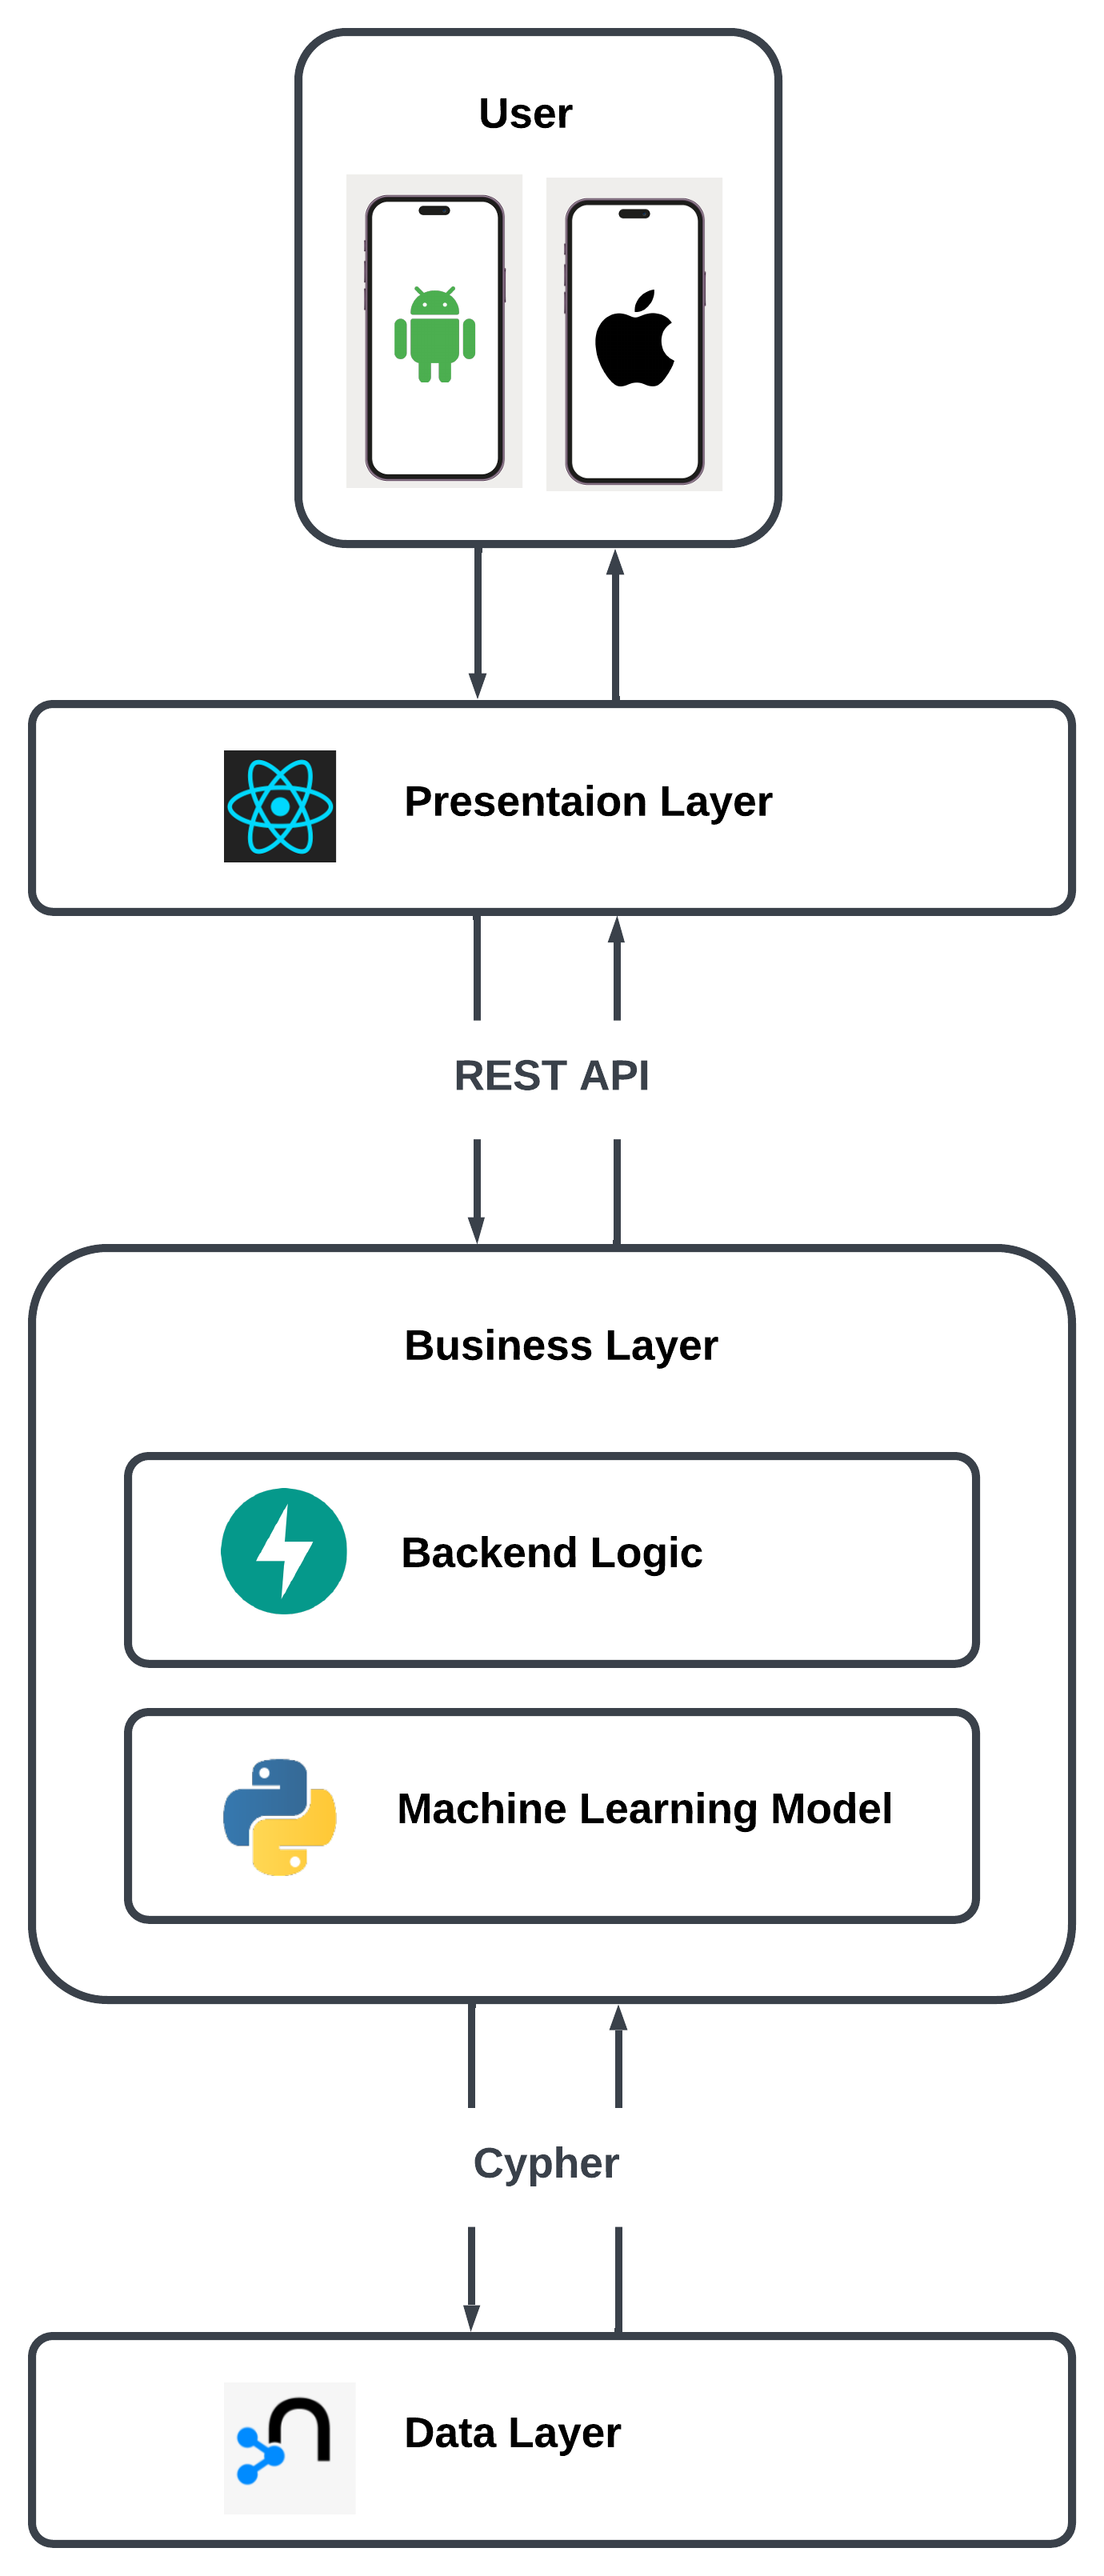
\includegraphics[width=7cm]{./Pictures/ArchDia.png}}
    \caption{Architecture diagram}\label{fig:ArchDia}
    \end{figure}

  จากภาพที่ \ref{fig:ArchDia} จะเป็นแผนภาพแสดงรายละเอียดโครงสร้างของระบบ เพื่อแสดงให้เห็นภาพรวมขององค์ประกอบและเครื่องมือต่าง ๆ ที่ใช้ในการพัฒนาแอปพลิเคชัน Actiwiz โดยตัวแอปพลิเคชันนั้นรองรับการทำงานทั้งในระบบปฏิบัติการทั้ง IOS และ Android โดยใน Presentation layer ถูกสร้างโดยใช้ react native ซึ่งสื่อสารกับ Business layer โดยอาศัย REST API Backend Logic ใช้ fast api ในการพัฒนา และทำการสร้าง Model การเรียนรู้ของเครื่องโดยใช้ Python ซึ่งจะใช้ Cypher ในการสื่อสารกับ Data layer ที่ถูกสร้างขึ้นด้วย Neo4j database
\newpage

ผังงานระบบ (System Flow)
\begin{enumerate}
  \item User ใช้งาน React Native Application
  \item React Native ส่ง HTTP request ตามรูปแบบของ Rest API ที่กำหนดไว้ ไปยัง FastAPI backend เพื่อเรียกใช้งานฟังก์ชันต่าง ๆ เช่น ค้นหากิจกรรมหรือดูข้อมูลเกี่ยวกับชมรม เป็นต้น
  \item FastAPI ประมวลผล request และส่ง request เพิ่มเติมด้วย Cypher ไปยัง Neo4j database เพื่อขอข้อมูล หรือเปลี่ยนแปลงข้อมูล
    สำหรับการแนะนำและการประมวลผลข้อมูลกิจกรรมหรือชมรม FastAPI จะติดต่อกับ Machine Learning Model เพิ่มเติม
  \item Neo4j ประมวลผลข้อมูลตาม request ของ FastAPI
  \item FastAPI ส่ง HTTP response กลับไปยัง React Native และ React Native ปรับเปลี่ยน User Interface ตาม response ที่ได้รับ
\end{enumerate}

\section{เเผนภาพที่ใช้เเสดงปฎิสัมพันธ์ระหว่างระบบงานเเละสิ่งที่อยู่นอกระบบงาน (Use Case Diagram)}

  \begin{figure}[!h]\centering
    \setlength{\fboxrule}{0.5mm} % can define this in the preamble
    \setlength{\fboxsep}{0.5cm}
    \fbox{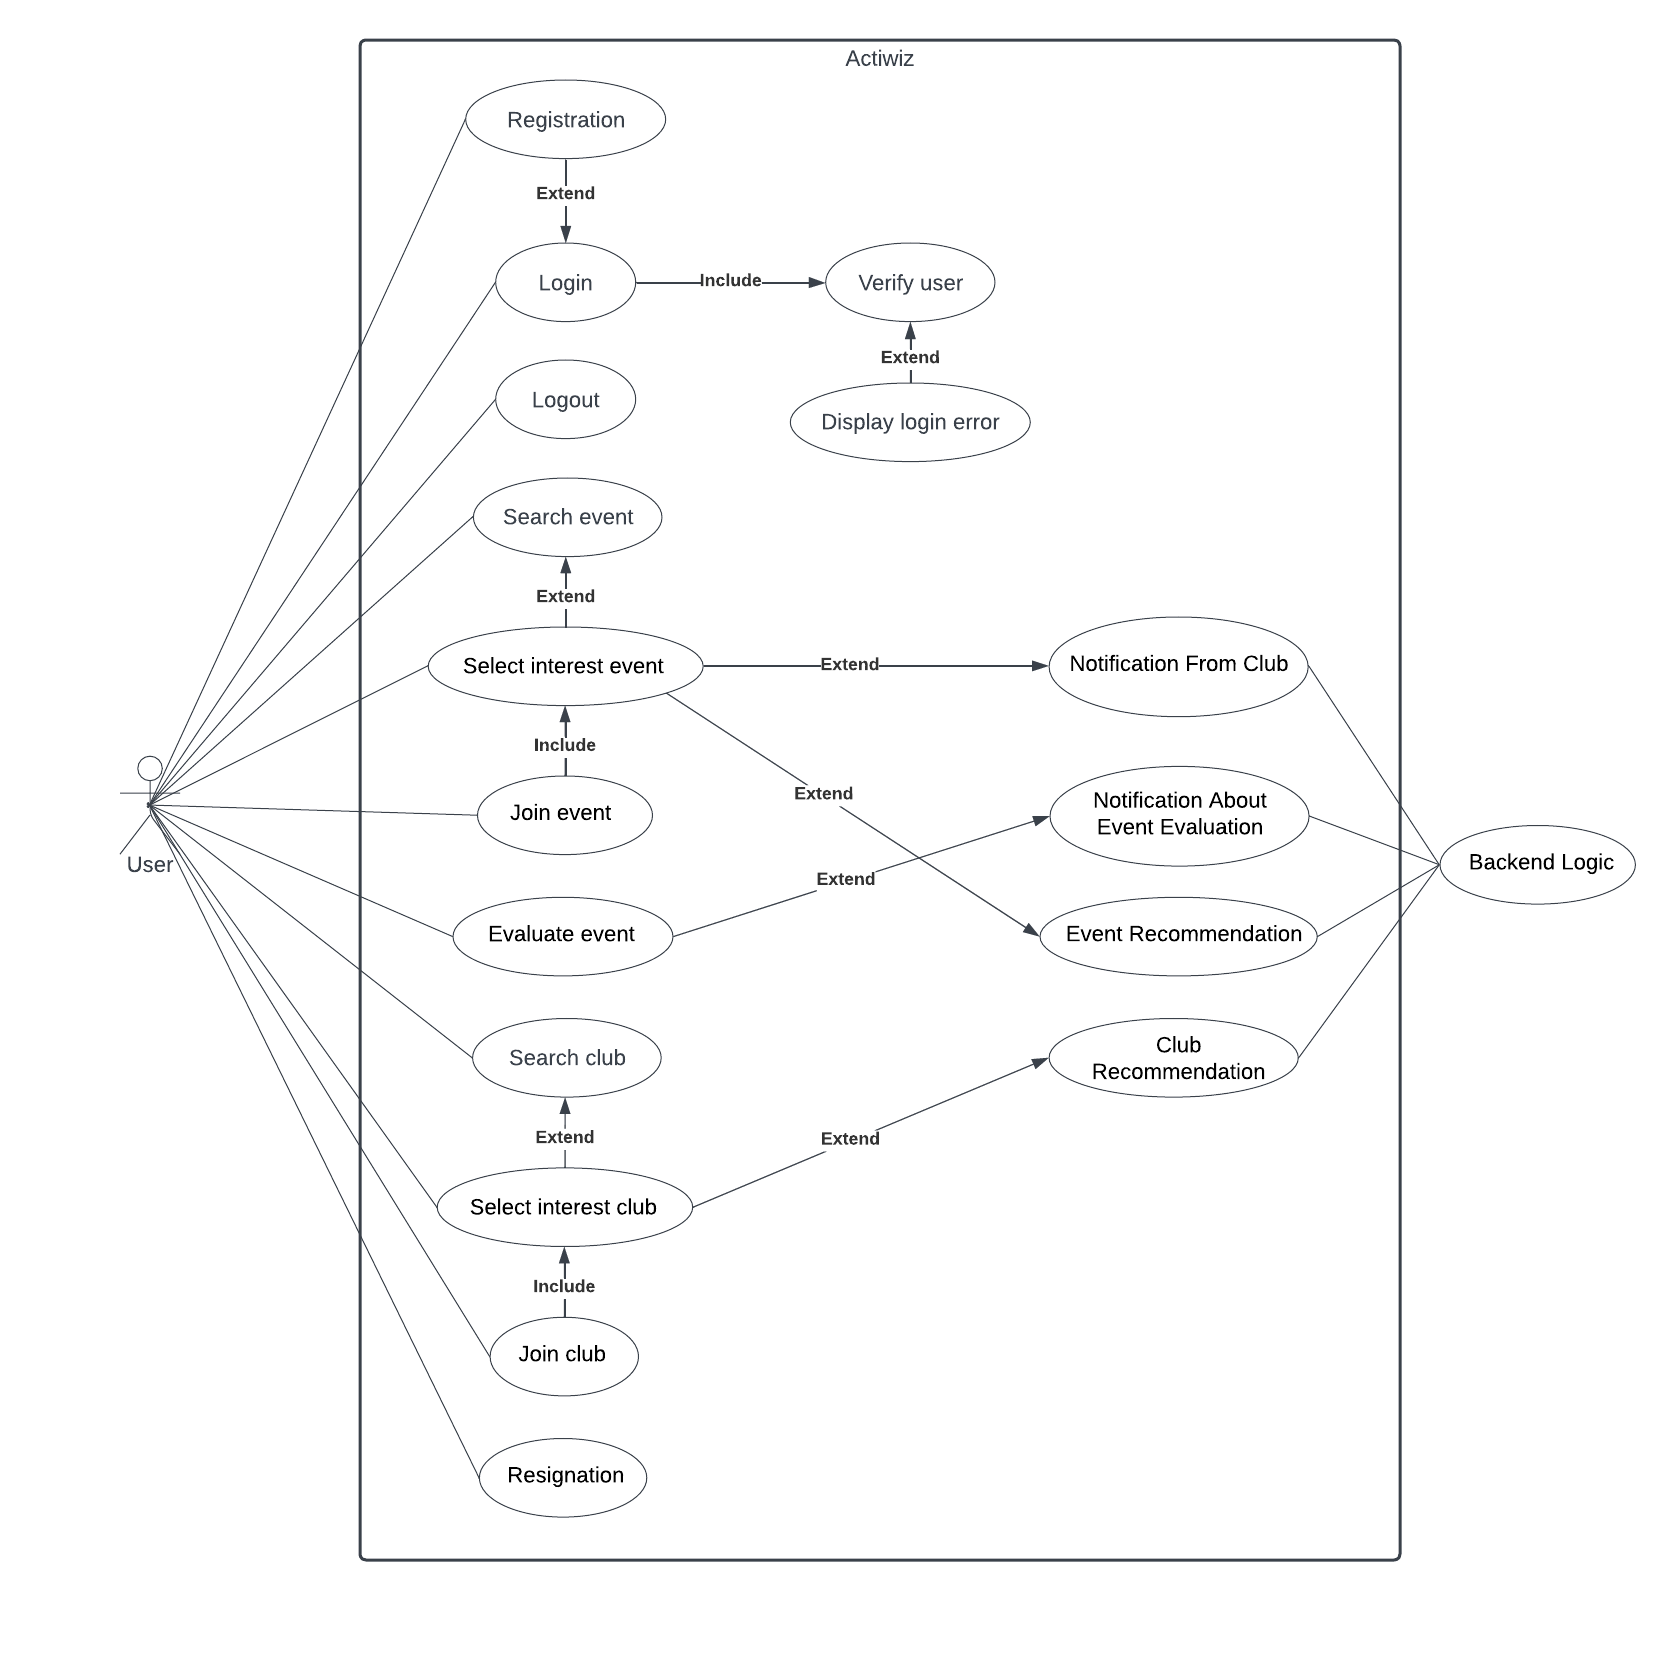
\includegraphics[width=13cm]{./Pictures/usedcase.png}}
    \caption{Use Case Diagram}\label{fig:usecasediagram}
  \end{figure}

  จากภาพที่ \ref{fig:usecasediagram} เป็นแผนภาพที่แสดงให้เห็นความสัมพันธ์ว่าแต่ละระบบมีความเกี่ยวข้องกันอย่างไรและผู้มีส่วนเกี่ยวข้องในระบบสามารถทำอะไรได้บ้าง โดยในฝั่งของผู้ใช้งานนั้นจะเริ่มตั้งแต่สามารถสมัครบัญชีการใช้งานได้ การที่เข้าสู่ระบบเพื่อใช้งานคุณลักษณะต่าง ๆ เช่น การค้นหา, อ่านรายละเอียดและเข้าร่วมกิจกรรม การประเมินกิจกรรม การค้นหา, เข้าร่วม และลาออกจากชมรม รวมถึงงานที่ระบบ Backend กระทำต่อระบบ ทั้งการแนะนำชมรมหรือกิจกรรม แจ้งเตือนกิจกรรมที่ชมรมจัดหรือการประเมินกิจกรรมที่เกิดขึ้น\\

\textbf{Use Case Narratives} 
ส่วนนี้จะเป็นการบรรยายให้รายละเอียดเกี่ยวกับกรณีการใช้งานระบบต่าง ๆ ในตัวแอปพลิเคชันที่ถูกเขียนไว้ในเเผนภาพที่ใช้เเสดงปฎิสัมพันธ์ระหว่างระบบงานเเละสิ่งที่อยู่นอกระบบงาน ทั้งเป้าหมายของผู้ใช้งาน, เงื่อนไขการใช้งาน และขั้นตอนต่าง ๆ ในกรณีใช้งานนั้นโดยละเอียด โดยจะแบ่งเป็น 3 ส่วนหลัก ได้แก่ 
\begin{enumerate}
  \item Goal หรือเป้าหมายของระบบ
  \item Pre-conditions หรือเงื่อนไขที่ต้องเกิดขั้นก่อนที่จะใช้งานระบบในกรณีใช้งานนั้นได้
  \item Main Success Scenario หรือขั้นตอนการใช้งานระบบในสถานการณ์ปกติ
\end{enumerate}
ซึ่งแอปพลิเคชั่นที่เป็นผลิตภัณฑ์ของโครงการมี นั้นมีผู้กระทำหลักคือ User และผู้กระทำรองคือ Backend Logic ซึ่งขั้นตอนที่เกิดขึ้นและเงื่อนไขในการเกิดขึ้นของแต่ล่ะกรณีใช้งานมีรายละเอียดดังที่ระบุไว้ในตารางดังต่อไปนี้

การสมัครเข้าใช้งาน
\begin{table}[!h]\centering
  \begin{tabular}{|c|c|}
  \hline
  \rowcolor[HTML]{9FC5E8} 
  Actor                       & {\color[HTML]{242424} User}                   \\ \hline
  \rowcolor[HTML]{FFFFFF} 
  {\color[HTML]{242424} Goal} & {\color[HTML]{242424} ลงทะเบียนสร้าง account} \\ \hline
  Pre-conditions              & -                                             \\ \hline
  Main success scenario & \begin{tabular}[c]{@{}l@{}}1.User ทำการกดเข้าหน้าลงทะเบียน\\ 2.User กรอกแบบฟอร์ม\\ 3.User กดยืนยันการสร้าง account\end{tabular} \\ \hline
  \end{tabular}
  \caption{\centering การสมัครเข้าใช้งาน}\label{tab:Registration scenario}
\end{table}

การเข้าสู่ระบบ

\begin{table}[!h]\centering
  \begin{tabular}{|c|c|}
  \hline
  \rowcolor[HTML]{9FC5E8} 
  Actor                       & {\color[HTML]{242424} User}                                                                                          \\ \hline
  \rowcolor[HTML]{FFFFFF} 
  {\color[HTML]{242424} Goal} & {\color[HTML]{242424} เข้าสู่ระบบและใช้งานฟังก์ชันต่างได้}                                                           \\ \hline
  Pre-conditions              & \begin{tabular}[c]{@{}c@{}}-User จำเป็นต้องลงทะเบียน account ก่อน\\ -User จำเป็นต้องยืนยัน account ก่อน\end{tabular} \\ \hline
  Main success scenario &
    \begin{tabular}[c]{@{}c@{}}1.User กรอกอีเมลและรหัสผ่าน\\ 2.User เข้าสู่ homepage ของแอปพลิเคชัน\\ 3.ระบบแสดงฟังก์ชันที่ใช้งานได้ทั้งหมด\\ 4.Userใช้งานฟังก์ชันต่าง ๆ ในแอปพลิเคชัน\end{tabular} \\ \hline
  \end{tabular}
  \caption{\centering การเข้าสู่ระบบ}\label{tab:Login scenario}
\end{table}

การออกจากระบบ

\begin{table}[!h]\centering
  \begin{tabular}{|c|c|}
  \hline
  \rowcolor[HTML]{9FC5E8} 
  Actor                       & {\color[HTML]{242424} User}       \\ \hline
  \rowcolor[HTML]{FFFFFF} 
  {\color[HTML]{242424} Goal} & {\color[HTML]{242424} ออกจากระบบ} \\ \hline
  Pre-conditions              & -User ต้องเข้าสู่ระบบก่อน         \\ \hline
  Main success scenario       & User ทำการกดออกจากระบบ            \\ \hline
  \end{tabular}
  \caption{\centering การออกจากระบบ}\label{tab:Logout scenario}
\end{table}

\newpage

การค้นหากิจกรรม

\begin{table}[!h]\centering
  \begin{tabular}{|c|c|}
  \hline
  \rowcolor[HTML]{9FC5E8} 
  Actor                       & {\color[HTML]{242424} User}         \\ \hline
  \rowcolor[HTML]{FFFFFF} 
  {\color[HTML]{242424} Goal} & {\color[HTML]{242424} ค้นหากิจกรรม} \\ \hline
  Pre-conditions              & - User ต้องเข้าสู่ระบบก่อน          \\ \hline
  Main success scenario & \begin{tabular}[c]{@{}c@{}}1.User ค้นหากิจกรรมที่ต้องการ\\ 2.ระบบแสดงกิจกรรมที่ค้นหา\end{tabular} \\ \hline
  \end{tabular}
  \caption{\centering การค้นหากิจกรรม}\label{tab:Search event scenario}
\end{table}

การอ่านรายละเอียดกิจกรรม

\begin{table}[!h]\centering
  \begin{tabular}{|c|c|}
  \hline
  \rowcolor[HTML]{9FC5E8} 
  Actor                       & {\color[HTML]{242424} User}                  \\ \hline
  \rowcolor[HTML]{FFFFFF} 
  {\color[HTML]{242424} Goal} & {\color[HTML]{242424} อ่านรายละเอียดกิจกรรม} \\ \hline
  Pre-conditions              & - User ต้องเข้าสู่ระบบก่อน                   \\ \hline
  Main success scenario & \begin{tabular}[c]{@{}c@{}}1.User กดไปที่กิจกรรมที่สนใจ\\ 2.ระบบแสดงรายละเอียดกิจกรรมที่ค้นหา\end{tabular} \\ \hline
  \end{tabular}
  \caption{\centering การอ่านรายละเอียดกิจกรรม}\label{tab:Select event scenario}
\end{table}

การเข้าร่วมกิจกรรม

\begin{table}[!h]\centering
  \begin{tabular}{|c|c|}
  \hline
  \rowcolor[HTML]{9FC5E8} 
  Actor                       & {\color[HTML]{242424} User}            \\ \hline
  \rowcolor[HTML]{FFFFFF} 
  {\color[HTML]{242424} Goal} & {\color[HTML]{242424} เข้าร่วมกิจกรรม} \\ \hline
  Pre-conditions        & \begin{tabular}[c]{@{}c@{}}- User ต้องเข้าสู่ระบบก่อน\\ - User ต้องเข้าสู่หน้าอ่านรายละเอียดกิจกรรมก่อน\end{tabular} \\ \hline
  Main success scenario & \begin{tabular}[c]{@{}c@{}}1.User กดเข้าร่วมกิจกรรม\\ 2.ระบบพาไปยังหน้ากรอกแบบฟอร์มของกิจกรรม\end{tabular}           \\ \hline
  \end{tabular}
  \caption{\centering การเข้าร่วมกิจกรรม}\label{fig:Join event scenario}
\end{table}

การประเมินกิจกรรม

\begin{table}[!h]\centering
  \begin{tabular}{|c|c|}
  \hline
  \rowcolor[HTML]{9FC5E8} 
  Actor                       & {\color[HTML]{242424} User}           \\ \hline
  \rowcolor[HTML]{FFFFFF} 
  {\color[HTML]{242424} Goal} & {\color[HTML]{242424} ประเมินกิจกรรม} \\ \hline
  Pre-conditions              & - User ต้องเข้าสู่ระบบก่อน            \\ \hline
  Main success scenario & \begin{tabular}[c]{@{}c@{}}1.User ได้รับแจ้งเตือนการประเมินกิจกรรม\\ 2.User กดเข้าประเมินกิจกรรม\\ 3.ระบบพาไปหน้าประเมินกิจกรรม\end{tabular} \\ \hline
  \end{tabular}
  \caption{\centering การประเมินกิจกรรม}\label{fig:Evaluate event scenario}
\end{table}

การค้นหาชมรม

\begin{table}[!h]\centering
  \begin{tabular}{|c|c|}
  \hline
  \rowcolor[HTML]{9FC5E8} 
  Actor                       & {\color[HTML]{242424} User}      \\ \hline
  \rowcolor[HTML]{FFFFFF} 
  {\color[HTML]{242424} Goal} & {\color[HTML]{242424} ค้นหาชมรม} \\ \hline
  Pre-conditions              & - User ต้องเข้าสู่ระบบก่อน       \\ \hline
  Main success scenario & \begin{tabular}[c]{@{}c@{}}1.User ค้นหาชมรมที่ต้องการ\\ 2.ระบบแสดงชมรมที่ค้นหา\end{tabular} \\ \hline
  \end{tabular}
  \caption{\centering การค้นหาชมรม}\label{fig:Search club scenario}
\end{table}

\newpage

การอ่านรายละเอียดชมรม

\begin{table}[!h]\centering
  \begin{tabular}{|c|c|}
  \hline
  \rowcolor[HTML]{9FC5E8} 
  Actor                       & {\color[HTML]{242424} User}               \\ \hline
  \rowcolor[HTML]{FFFFFF} 
  {\color[HTML]{242424} Goal} & {\color[HTML]{242424} อ่านรายละเอียดชมรม} \\ \hline
  Pre-conditions              & - User ต้องเข้าสู่ระบบก่อน                \\ \hline
  Main success scenario & \begin{tabular}[c]{@{}c@{}}1.User กดไปที่ชมรมที่สนใจ\\ 2.ระบบแสดงรายละเอียดชมรมที่ค้นหา\end{tabular} \\ \hline
  \end{tabular}
  \caption{\centering การอ่านรายละเอียดชมรม}\label{fig:Select club scenario}
\end{table}

การสมัครชมรม

\begin{table}[!h]\centering
  \begin{tabular}{|c|c|}
  \hline
  \rowcolor[HTML]{9FC5E8} 
  Actor                       & {\color[HTML]{242424} User}         \\ \hline
  \rowcolor[HTML]{FFFFFF} 
  {\color[HTML]{242424} Goal} & {\color[HTML]{242424} เข้าร่วมชมรม} \\ \hline
  Pre-conditions & \begin{tabular}[c]{@{}c@{}}- User ต้องเข้าสู่ระบบก่อน\\ - User ต้องเข้าสู่หน้าอ่านรายละเอียดชมรมก่อน\end{tabular} \\ \hline
  Main success scenario       & User กดเข้าร่วมชมรม                 \\ \hline
  \end{tabular}
  \caption{\centering การสมัครชมรม}\label{fig:Join club scenario}
\end{table}

การลาออกจากชมรม

\begin{table}[!h]\centering
  \begin{tabular}{|c|c|}
  \hline
  \rowcolor[HTML]{9FC5E8} 
  Actor                       & {\color[HTML]{242424} User}         \\ \hline
  \rowcolor[HTML]{FFFFFF} 
  {\color[HTML]{242424} Goal} & {\color[HTML]{242424} เข้าร่วมชมรม} \\ \hline
  Pre-conditions & \begin{tabular}[c]{@{}c@{}}- User ต้องเข้าสู่ระบบก่อน\\ - User ต้องเข้าสู่หน้าอ่านรายละเอียดชมรมก่อน\end{tabular} \\ \hline
  Main success scenario       & User กดเข้าร่วมชมรม                 \\ \hline
  \end{tabular}
  \caption{\centering การลาออกจากชมรม}\label{fig:Resignation scenario}
\end{table}

\newpage

\section{Sequence diagram}
\subsection{การเข้าสู่ระบบ}

  \begin{figure}[!h]\centering
    \setlength{\fboxrule}{0.5mm} % can define this in the preamble
    \setlength{\fboxsep}{0.5cm}
    \fbox{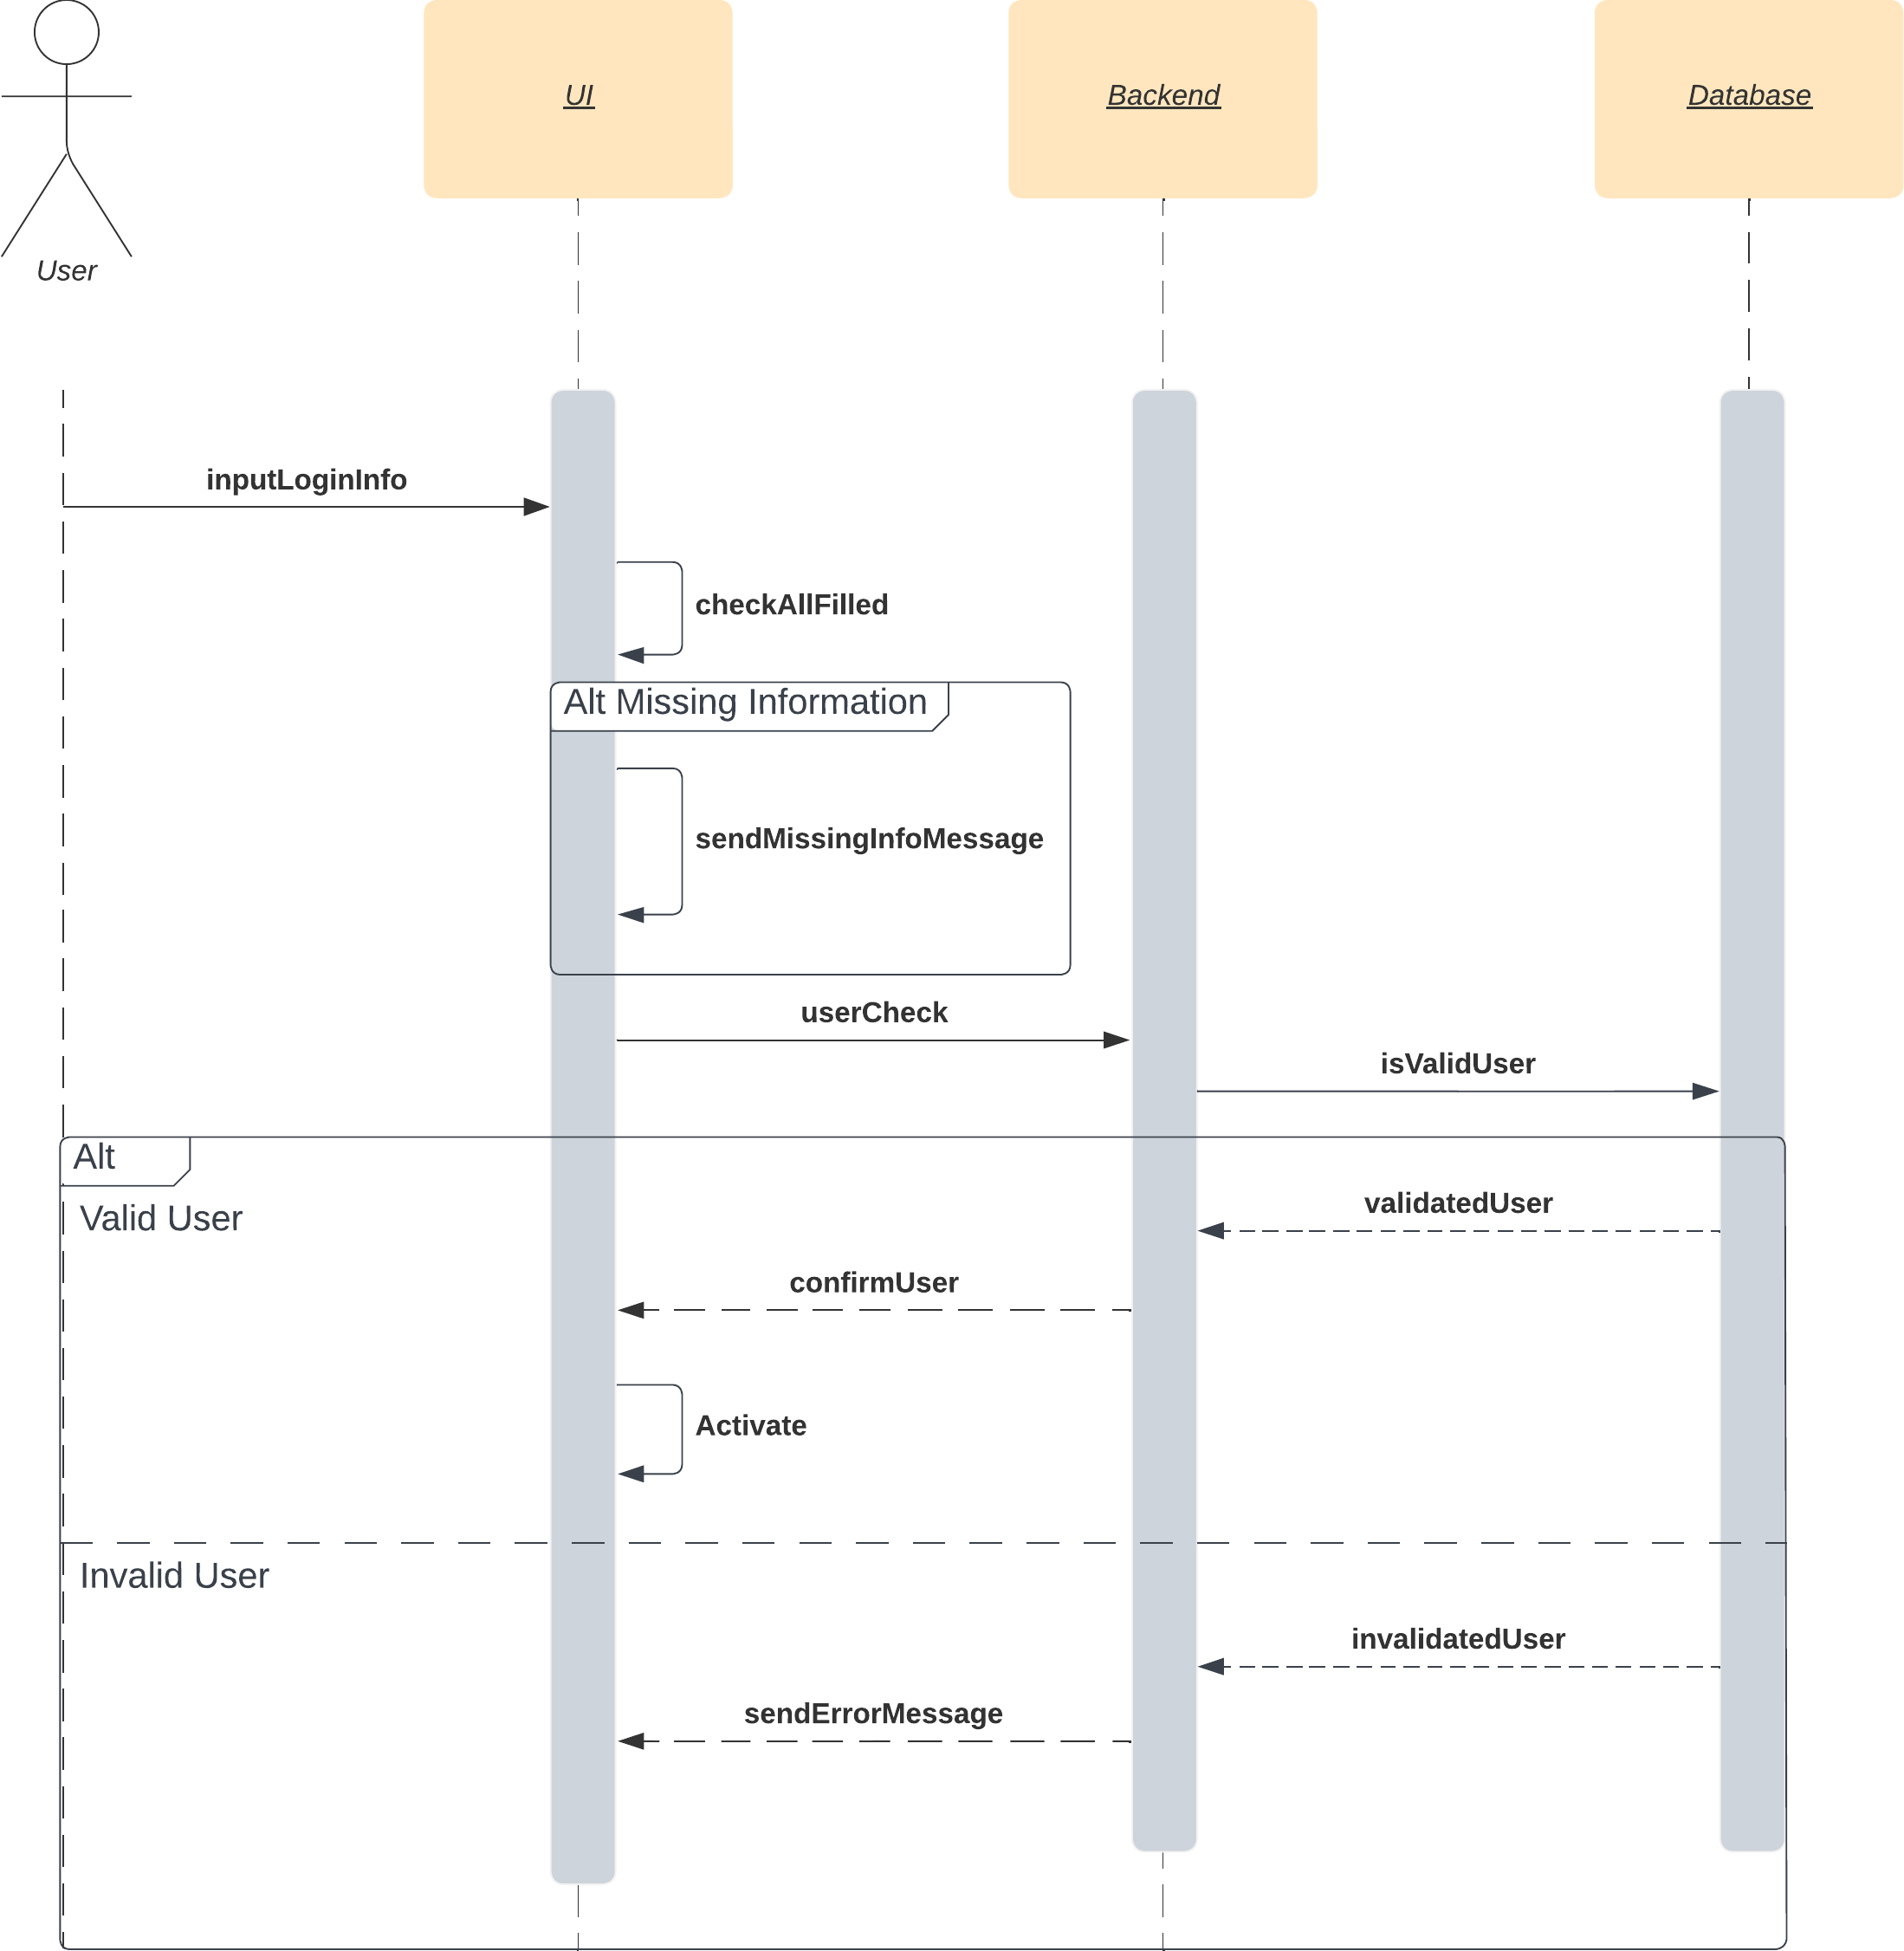
\includegraphics[width=12cm]{./Pictures/login.png}}
    \caption{\centering Sequence diagram ของการเข้าสู่ระบบ}\label{fig:Sequence diagram ของ login}
  \end{figure}

จากภาพ Sequence Diagram ในรูปที่\ref{fig:Sequence diagram ของ login} แสดงขั้นตอนการทำงานของระบบเมื่อผู้ใช้งานต้องการเข้าสู่ระบบ โดยมีรายละเอียดดังนี้
  \begin{enumerate}
    \item ผู้ใช้งานเริ่มต้นโดยการกรอกข้อมูลที่ใช้ในการเข้าสู่ระบบ (เช่น ชื่อผู้ใช้และรหัสผ่าน) ลงในหน้า Log in ของ User Interface (UI)
    \item เมื่อผู้ใช้งานกรอกข้อมูลเรียบร้อยแล้ว UI จะทำการตรวจสอบความถูกต้องและความครบถ้วนของข้อมูลที่ผู้ใช้งานกรอก หากพบว่าขาดข้อมูลบางส่วน UI จะแจ้งให้ผู้ใช้งานทราบและให้กรอกข้อมูลให้ครบถ้วน
    \item เมื่อข้อมูลที่จำเป็นสำหรับการเข้าสู่ระบบครบถ้วนแล้ว UI จะส่งข้อมูลดังกล่าวไปยัง Backend System
    \item Backend System จะเรียกข้อมูลจาก Database เพื่อตรวจสอบว่าข้อมูลที่ผู้ใช้งานกรอกมานั้นถูกต้องและตรงกับข้อมูลผู้ใช้งานที่มีอยู่ในระบบหรือไม่
    \item หากการตรวจสอบผ่าน Backend System จะแจ้งกลับไปยัง UI ว่าผู้ใช้งานสามารถเข้าสู่ระบบได้
    \item UI จะแสดงหน้าจอหลักของระบบให้กับผู้ใช้งาน เพื่อให้ผู้ใช้งานสามารถใช้งานฟังก์ชันต่าง ๆ ของระบบได้ต่อไป
  \end{enumerate}
  โดยสรุป Sequence Diagram นี้แสดงให้เห็นถึงขั้นตอนการทำงานร่วมกันระหว่าง User Interface, Backend System และ Database ในการตรวจสอบและยืนยันตัวตนของผู้ใช้งาน เพื่อให้ผู้ใช้งานสามารถเข้าสู่ระบบและใช้งานฟังก์ชันต่าง ๆ ของระบบได้อย่างถูกต้อง

\newpage

\subsection{การสมัครเข้าใช้งาน}

  \begin{figure}[!h]\centering
    \setlength{\fboxrule}{0.5mm} % can define this in the preamble
    \setlength{\fboxsep}{0.5cm}
    \fbox{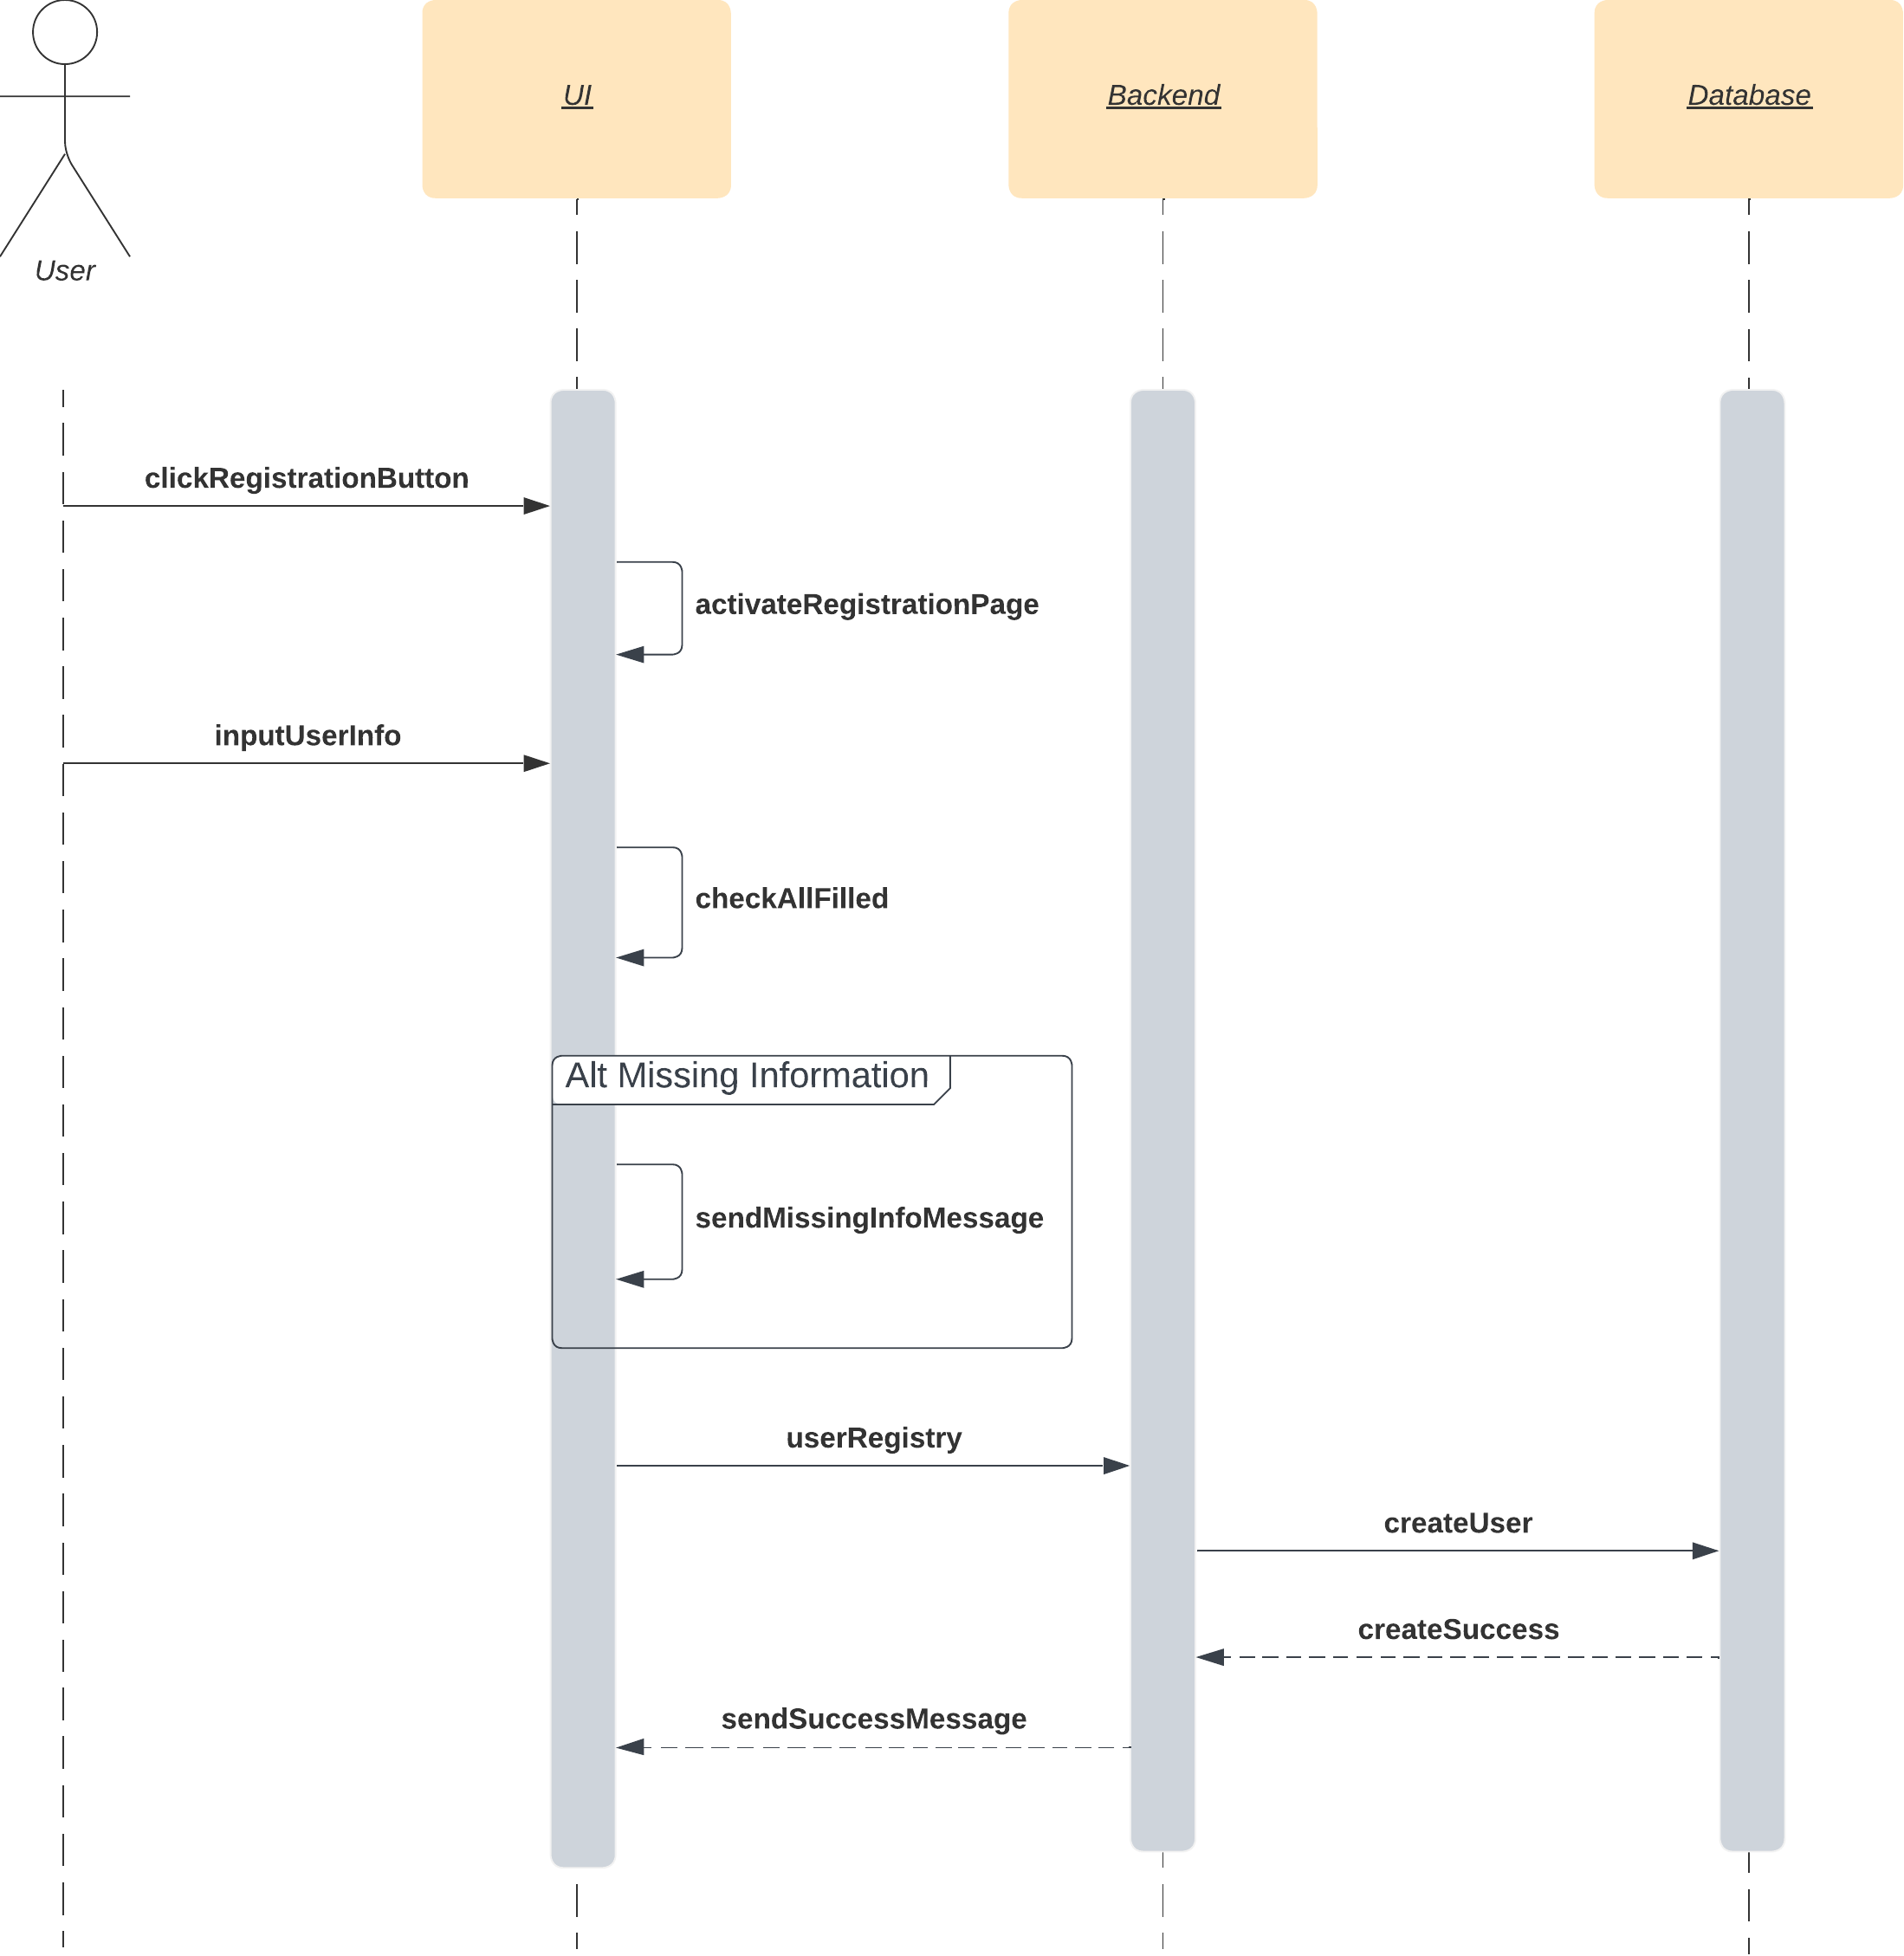
\includegraphics[width=12cm]{./Pictures/regis.png}}
    \caption{\centering การสมัครเข้าใช้งาน}\label{fig:regis}
  \end{figure}


จากภาพ Sequence Diagram ในรูปที่ \ref{fig:regis} แสดงขั้นตอนการทำงานของระบบเมื่อผู้ใช้งานต้องการสมัครเข้าใช้งานระบบ โดยมีรายละเอียดดังนี้
\begin{enumerate}
  \item ผู้ใช้งานเริ่มต้นโดยการกดปุ่มสมัครเข้าใช้งานบนหน้า User Interface (UI) ของระบบ
  \item หลังจากผู้ใช้งานกดปุ่มสมัครเข้าใช้งาน UI จะแสดงหน้าจอสำหรับให้ผู้ใช้งานกรอกข้อมูลที่จำเป็นในการสมัครสมาชิก เช่น ชื่อผู้ใช้งาน รหัสผ่าน อีเมล ฯลฯ
  \item เมื่อผู้ใช้งานกรอกข้อมูลเรียบร้อยแล้ว UI จะทำการตรวจสอบความถูกต้องและความครบถ้วนของข้อมูลที่ผู้ใช้งานกรอก หากพบว่าขาดข้อมูลบางส่วน UI จะแจ้งให้ผู้ใช้งานทราบและให้กรอกข้อมูลให้ครบถ้วน
  \item เมื่อข้อมูลที่จำเป็นสำหรับการสมัครสมาชิกครบถ้วนแล้ว UI จะส่งข้อมูลดังกล่าวไปยัง Backend System
  \item Backend System จะบันทึกข้อมูลผู้ใช้งานรายใหม่ลงใน Database
  \item หลังจากบันทึกข้อมูลเสร็จสิ้น Backend System จะส่งข้อความยืนยันการสมัครสมาชิกสำเร็จกลับไปยัง UI
  \item UI จะแสดงข้อความยืนยันการสมัครสมาชิกสำเร็จให้ผู้ใช้งานทราบ
\end{enumerate}
โดยสรุป Sequence Diagram นี้แสดงให้เห็นถึงขั้นตอนการทำงานร่วมกันระหว่าง User Interface, Backend System และ Database ในการรับข้อมูลการสมัครสมาชิกจากผู้ใช้งาน ตรวจสอบความถูกต้องและความครบถ้วนของข้อมูล บันทึกข้อมูลลงใน Database และแจ้งผลการสมัครสมาชิกกลับไปยังผู้ใช้งาน

\newpage


\subsection{การออกจากระบบ}

  \begin{figure}[!h]\centering
    \setlength{\fboxrule}{0.5mm} % can define this in the preamble
    \setlength{\fboxsep}{0.5cm}
    \fbox{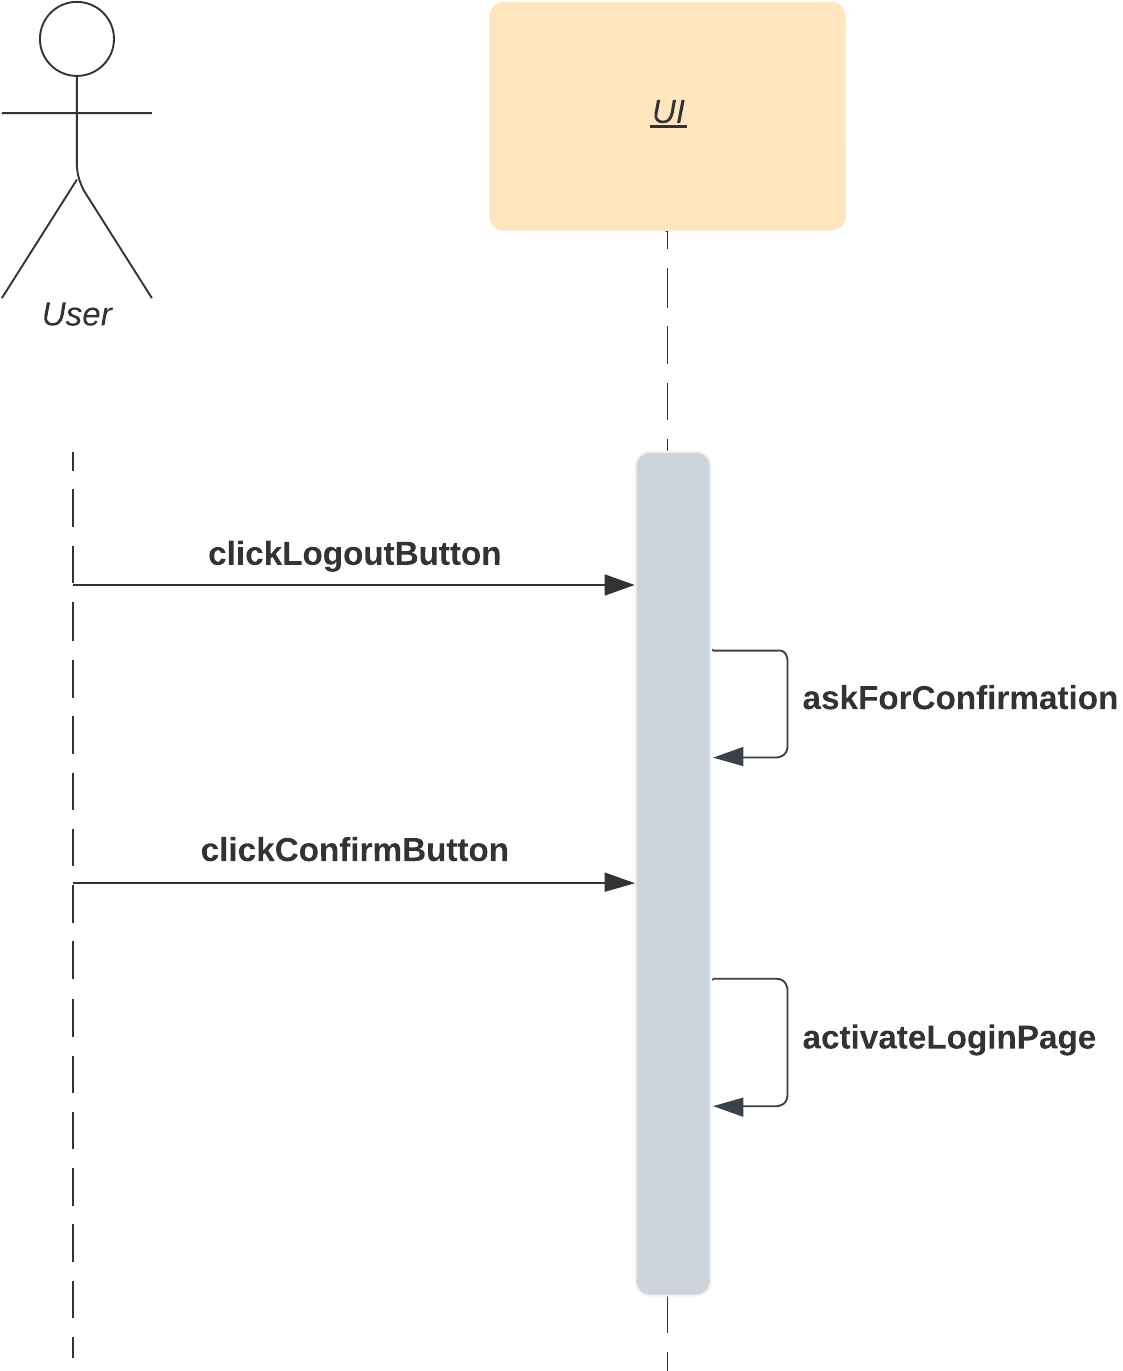
\includegraphics[width=12cm]{./Pictures/logout.png}}
    \caption{การออกจากระบบ}\label{fig:logout}
  \end{figure} 

  จากภาพ Sequence Diagram ในรูปที่ \ref{fig:logout} แสดงขั้นตอนการทำงานของระบบเมื่อผู้ใช้งานต้องการออกจากระบบ โดยมีรายละเอียดดังนี้
  \begin{enumerate}
    \item ผู้ใช้งานเริ่มต้นโดยการกดปุ่มออกจากระบบ (Log Out) บนหน้า User Interface (UI) ของระบบ
    \item หลังจากผู้ใช้งานกดปุ่มออกจากระบบ UI จะแสดงหน้าจอยืนยันการออกจากระบบ (Confirm Log Out) ให้ผู้ใช้งานอีกครั้ง เพื่อป้องกันการออกจากระบบโดยไม่ได้ตั้งใจ
    \item หากผู้ใช้งานยืนยันการออกจากระบบ UI จะส่งคำสั่งออกจากระบบไปยัง Backend System
    \item Backend System จะทำการปิดการเชื่อมต่อ (Session) ของผู้ใช้งานรายนั้นกับระบบ และลบข้อมูลการเข้าสู่ระบบ (Log Out) ของผู้ใช้งานออกจากระบบ
    \item หลังจากออกจากระบบเสร็จสิ้น Backend System จะแจ้งผลการออกจากระบบกลับไปยัง UI
    \item UI จะนำพาผู้ใช้งานกลับไปยังหน้าจอเข้าสู่ระบบ (Log In) เพื่อให้ผู้ใช้งานสามารถเข้าสู่ระบบใหม่ได้อีกครั้ง
  \end{enumerate}
  โดยสรุป Sequence Diagram นี้แสดงให้เห็นถึงขั้นตอนการทำงานร่วมกันระหว่าง User Interface และ Backend System ในการดำเนินการออกจากระบบของผู้ใช้งาน โดยมีการยืนยันการออกจากระบบจากผู้ใช้งานก่อน เพื่อป้องกันการออกจากระบบโดยไม่ได้ตั้งใจ หลังจากนั้น Backend System จะปิดการเชื่อมต่อและลบข้อมูลการเข้าสู่ระบบของผู้ใช้งานออกจากระบบ และนำผู้ใช้งานกลับไปยังหน้าจอเข้าสู่ระบบ

\newpage

\subsection{การค้นหากิจกรรม}

  \begin{figure}[!h]\centering
    \setlength{\fboxrule}{0.5mm} % can define this in the preamble
    \setlength{\fboxsep}{0.5cm}
    \fbox{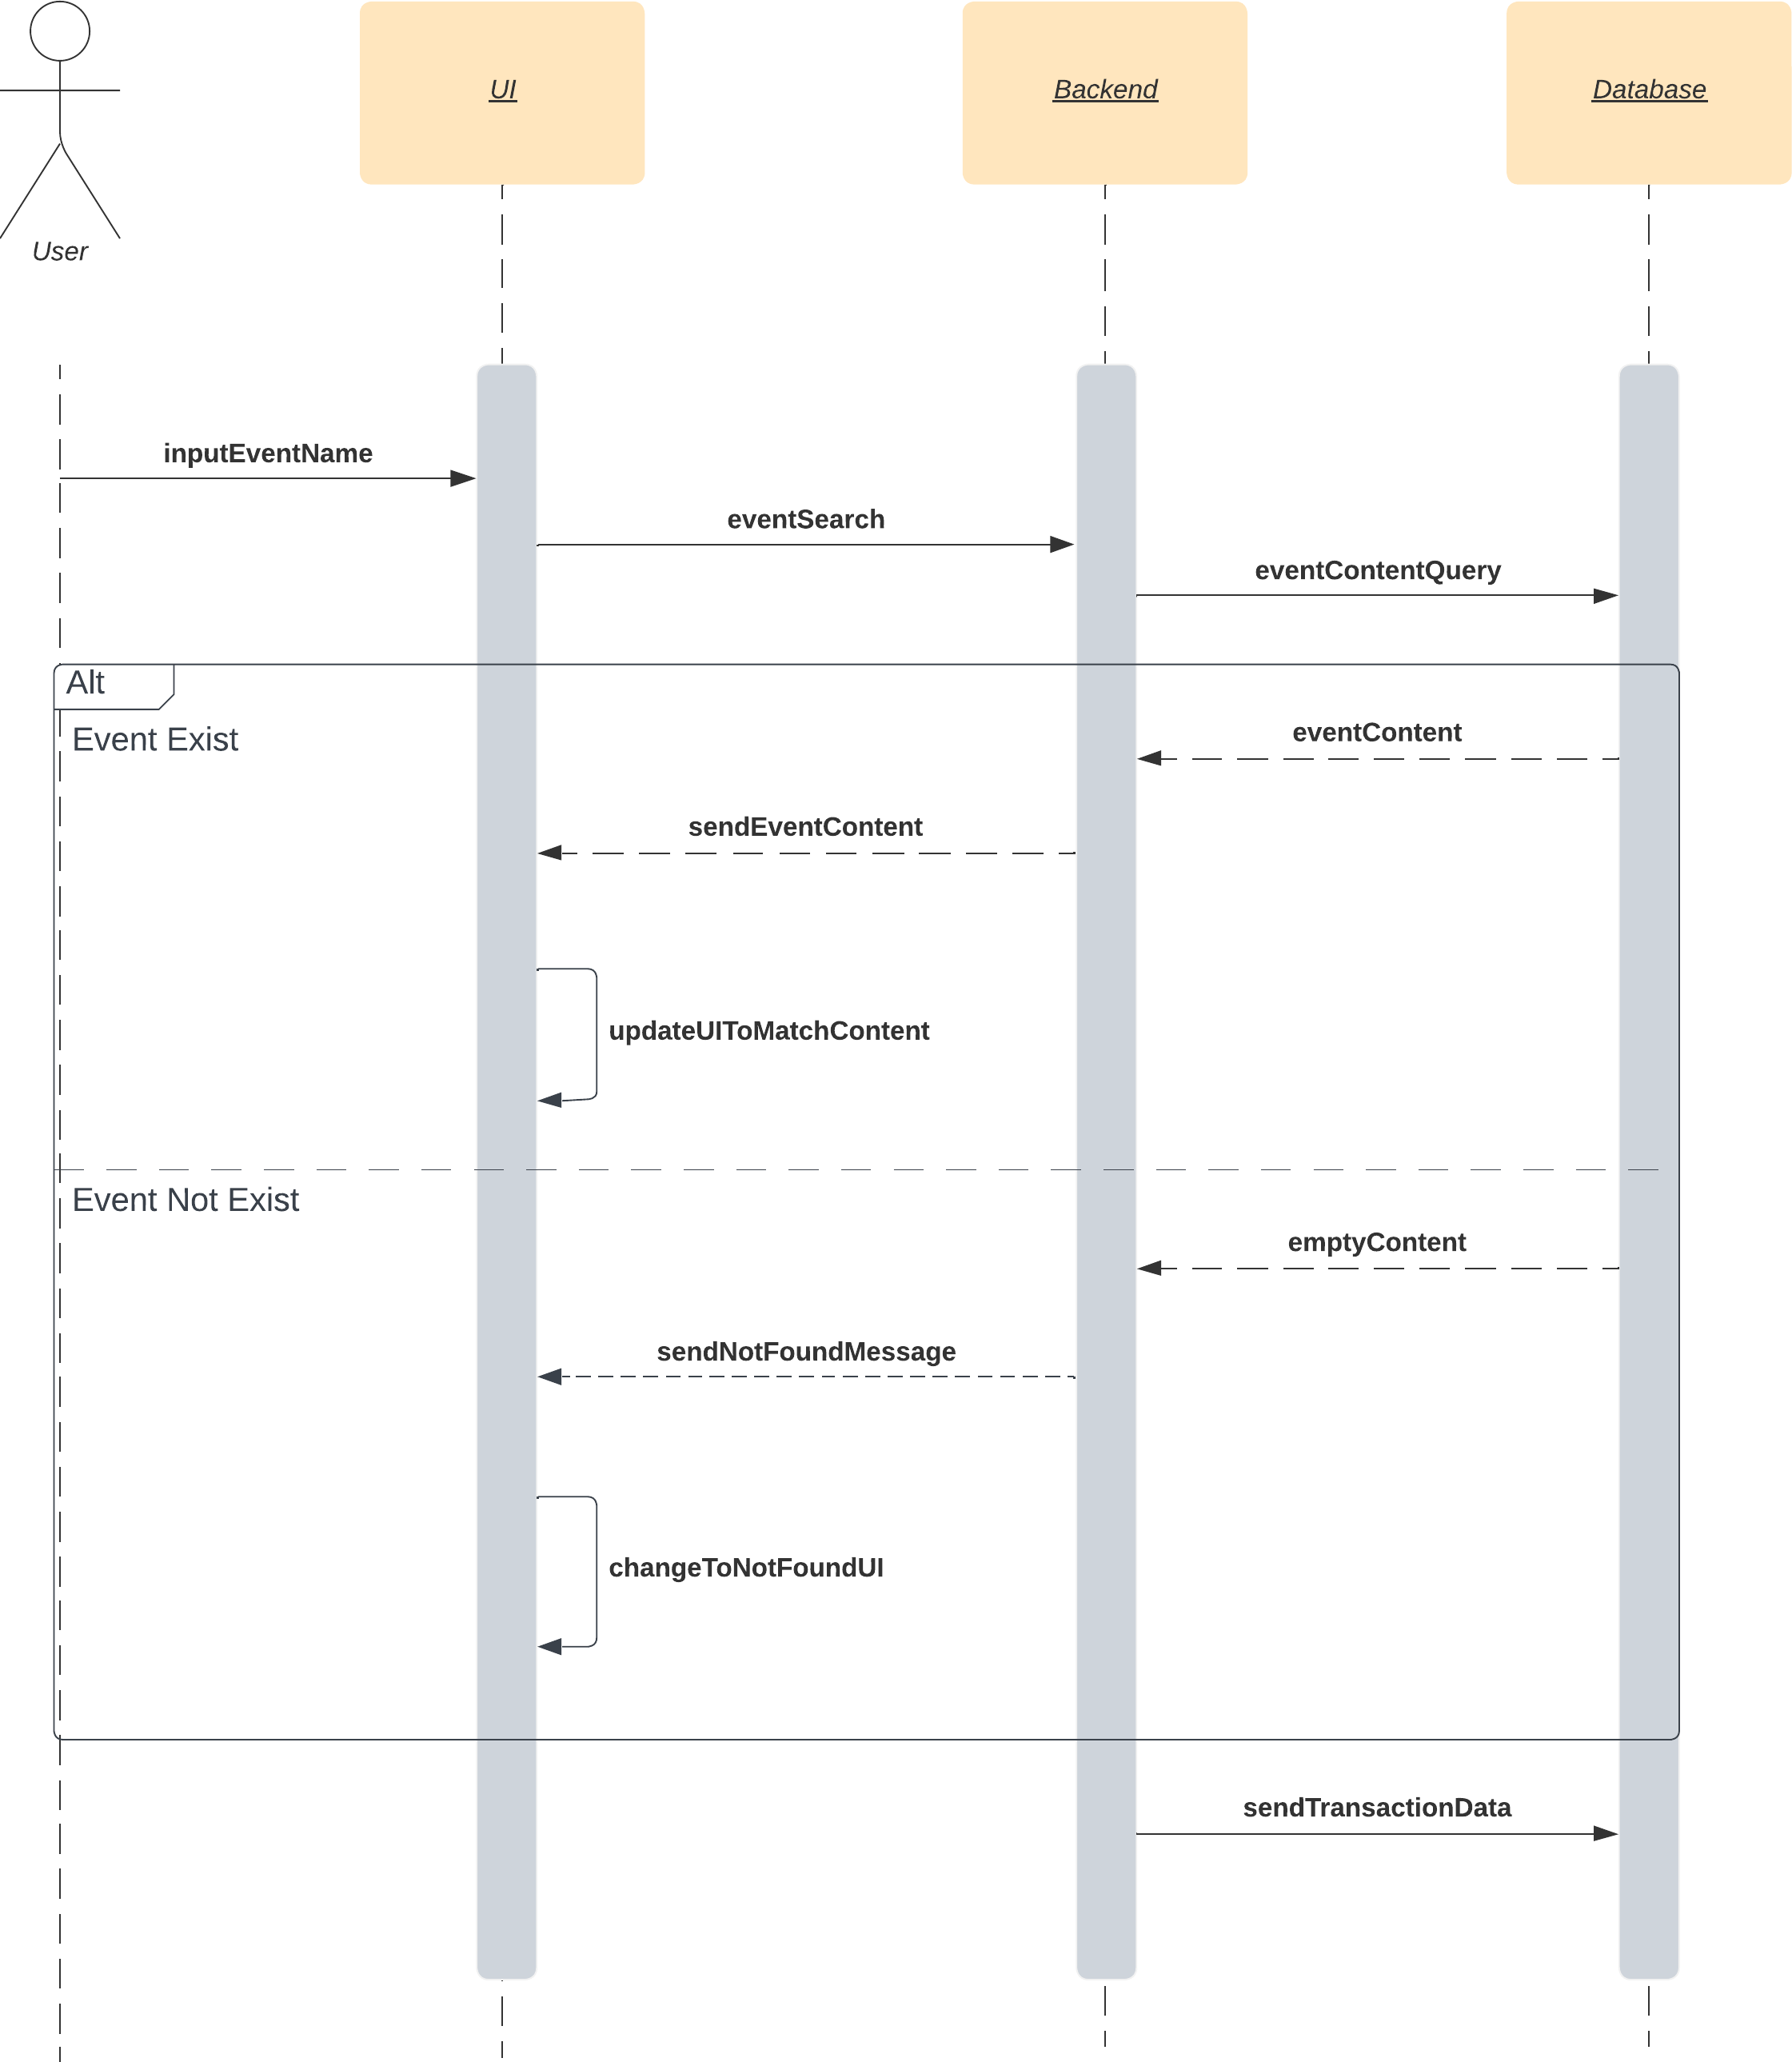
\includegraphics[width=10cm]{./Pictures/searchev.png}}
    \caption{การค้นหากิจกรรม}\label{fig:Search Event}
  \end{figure}

  จากภาพ Sequence Diagram ในรูปที่ \ref{fig:Search Event} แสดงขั้นตอนการทำงานของระบบเมื่อผู้ใช้งานต้องการค้นหากิจกรรม โดยมีรายละเอียดดังนี้
  \begin{enumerate}
    \item ผู้ใช้งานเริ่มต้นโดยการป้อนคำค้นหาหรือเงื่อนไขที่ต้องการค้นหากิจกรรมลงในช่องค้นหาบนหน้า User Interface (UI) ของระบบ
    \item หลังจากผู้ใช้งานป้อนคำค้นหาเรียบร้อยแล้ว UI จะส่งคำค้นหาหรือเงื่อนไขดังกล่าวไปยัง Backend System
    \item Backend System จะทำการค้นหาข้อมูลกิจกรรมที่ตรงกับคำค้นหาหรือเงื่อนไขที่ได้รับมาจาก Database
    \item หากพบข้อมูลกิจกรรมที่ตรงกับคำค้นหาหรือเงื่อนไข Backend System จะส่งข้อมูลกิจกรรมเหล่านั้นกลับไปยัง UI
    \item UI จะแสดงข้อมูลกิจกรรมที่ค้นหาได้ให้ผู้ใช้งานเห็น
    \item หากไม่พบข้อมูลกิจกรรมที่ตรงกับคำค้นหาหรือเงื่อนไข Backend System จะแจ้งกลับไปยัง UI ว่าไม่พบข้อมูลกิจกรรมที่ค้นหา
    \item UI จะแสดงข้อความ "ไม่พบกิจกรรมที่ค้นหา" ให้ผู้ใช้งานทราบ
    \item นอกจากนี้ Backend System จะบันทึกข้อมูลการค้นหาของผู้ใช้งานลงใน Database ด้วย ไม่ว่าการค้นหานั้นจะประสบความสำเร็จหรือไม่ก็ตาม
  \end{enumerate}
  โดยสรุป Sequence Diagram นี้แสดงให้เห็นถึงขั้นตอนการทำงานร่วมกันระหว่าง User Interface, Backend System และ Database ในการค้นหาข้อมูลกิจกรรมตามคำค้นหาหรือเงื่อนไขที่ผู้ใช้งานต้องการ โดยจะแสดงผลการค้นหาให้ผู้ใช้งานทราบ และบันทึกข้อมูลการค้นหาลงใน Database ไม่ว่าผลการค้นหาจะสำเร็จหรือไม่ก็ตาม

  \newpage

\subsection{การอ่านรายละเอียดของกิจกรรมและเข้าร่วมกิจกรรม}

  \begin{figure}[!h]\centering
    \setlength{\fboxrule}{0.5mm} % can define this in the preamble
    \setlength{\fboxsep}{0.5cm}
    \fbox{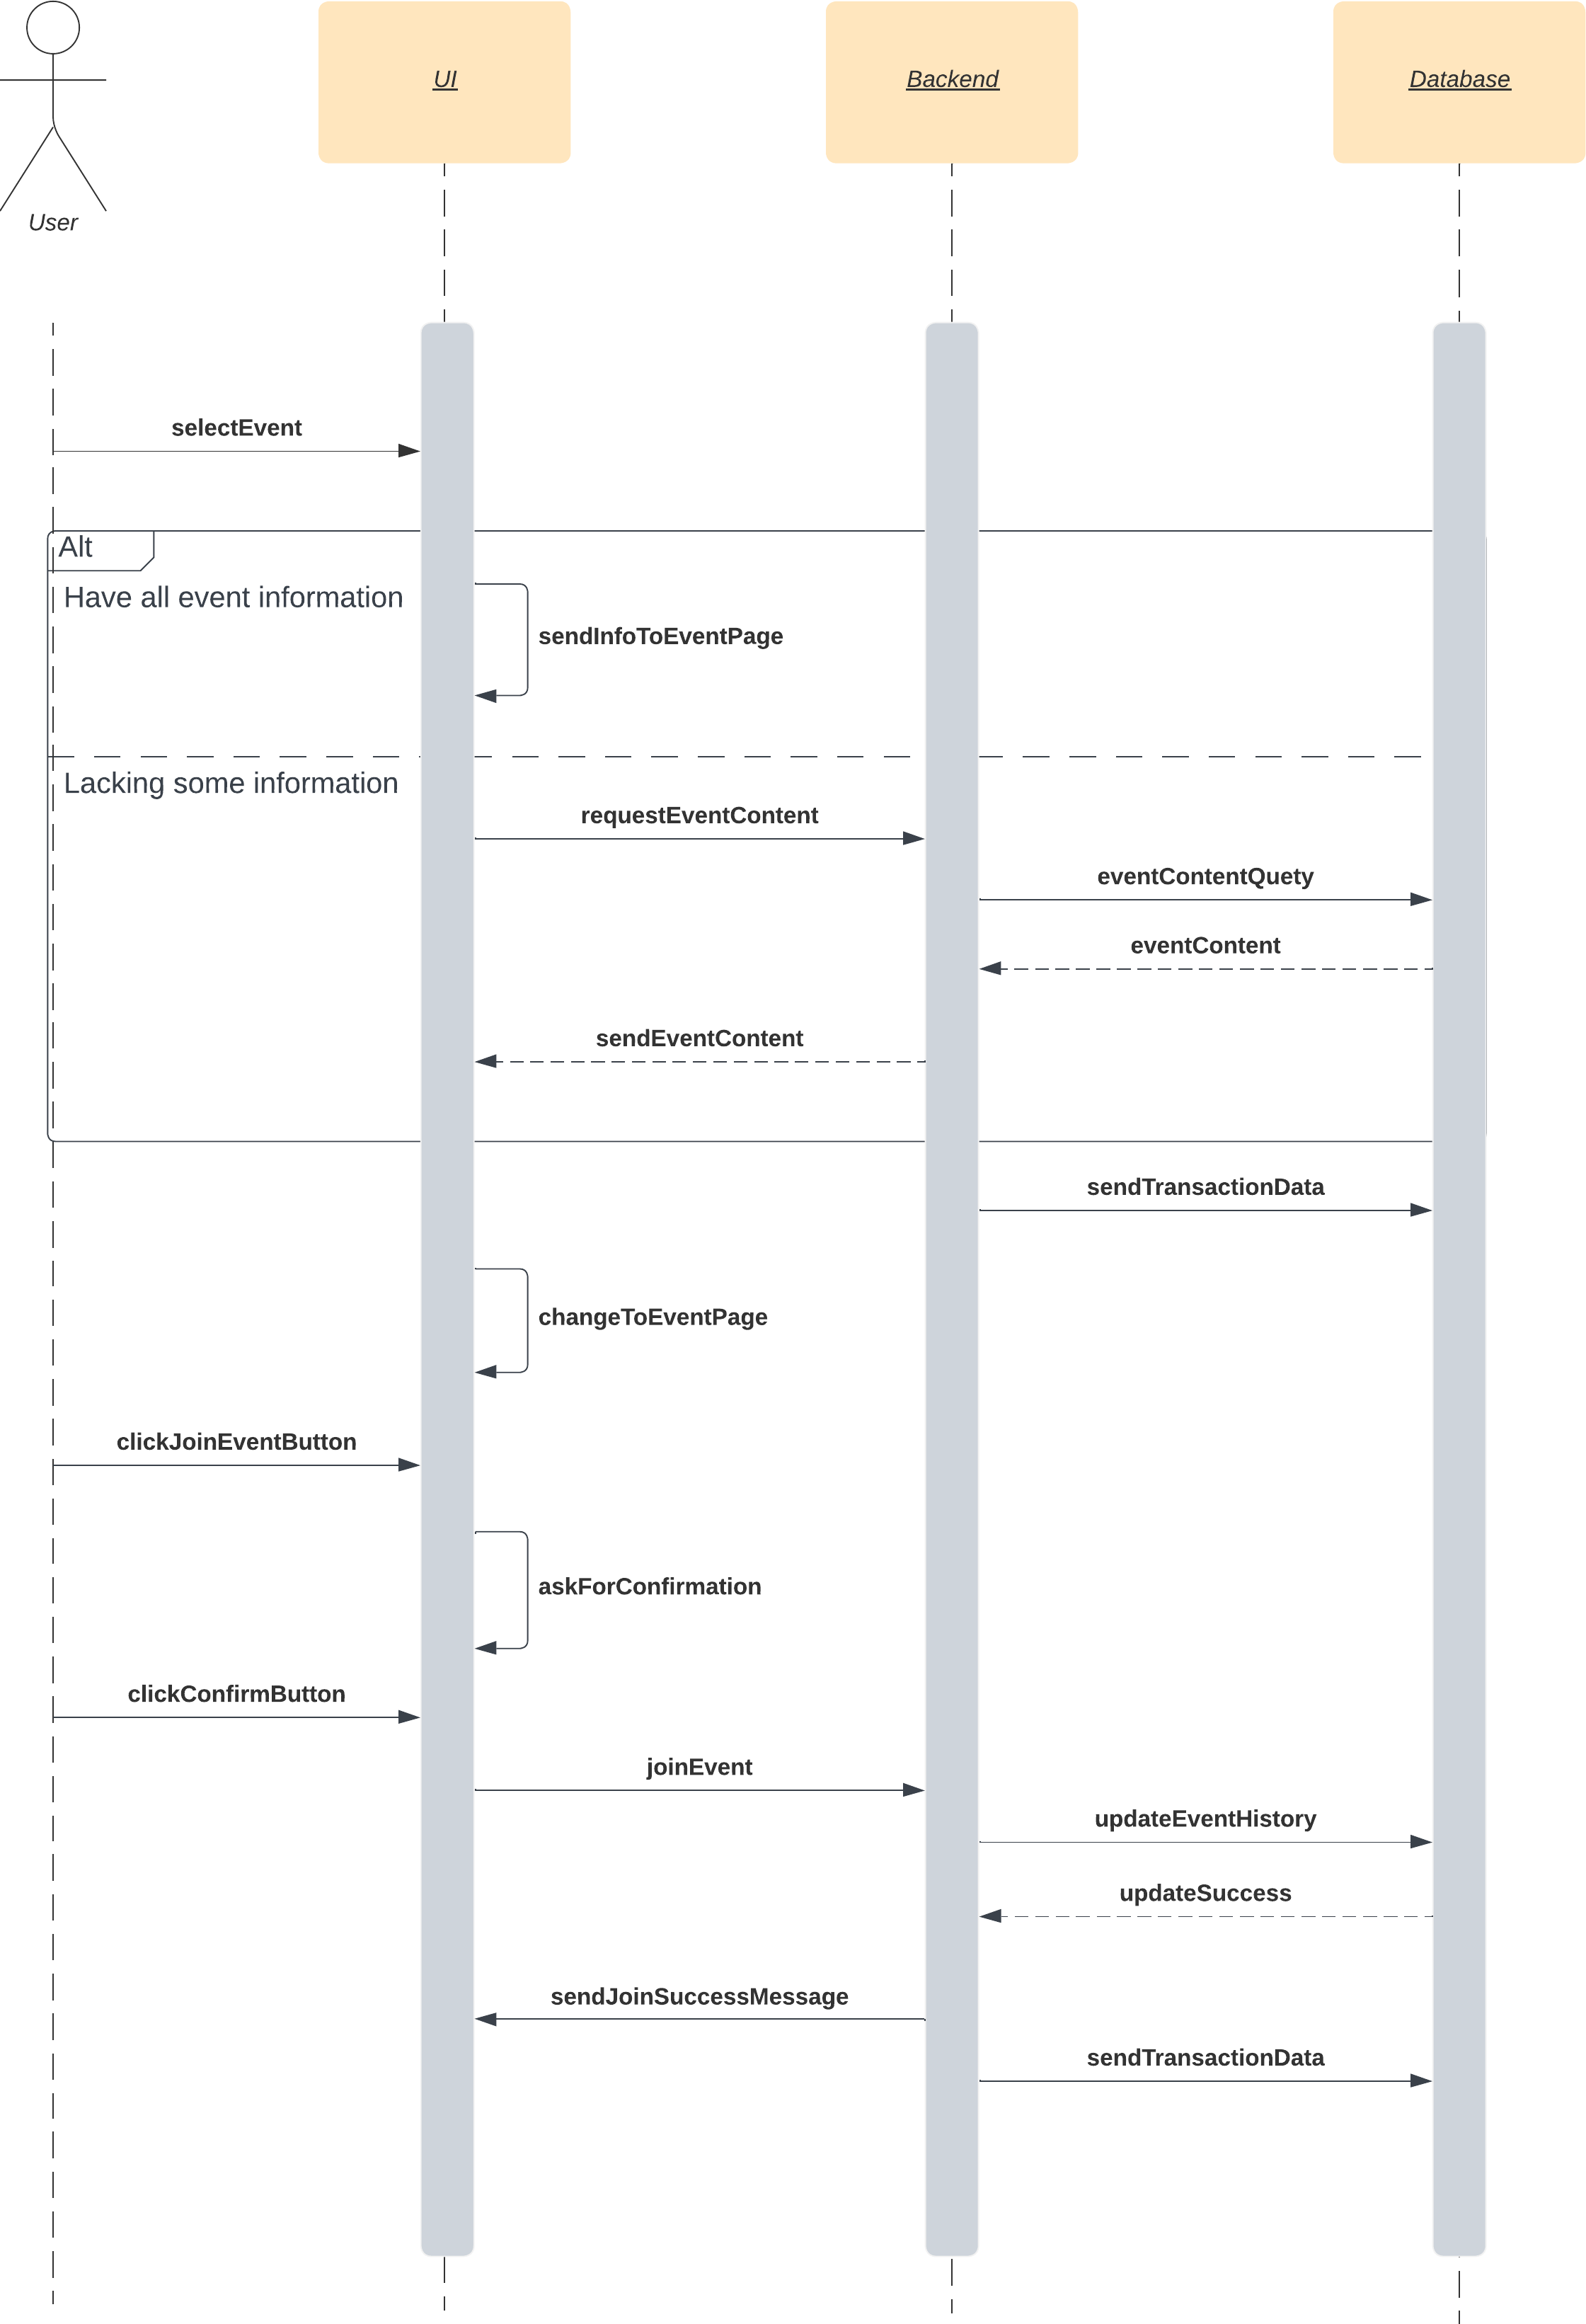
\includegraphics[width=10cm]{./Pictures/selectandjoin.png}}
    \caption{การอ่านรายละเอียดของกิจกรรมและเข้าร่วมกิจกรรม}\label{fig:Select and join event}
  \end{figure}

  จากภาพ Sequence Diagram ในรูปที่ \ref{fig:Select and join event} แสดงขั้นตอนการทำงานของระบบเมื่อผู้ใช้งานต้องการอ่านรายละเอียดของกิจกรรม และเข้าร่วมกิจกรรมนั้น โดยมีรายละเอียดดังนี้
  \begin{enumerate}
    \item ผู้ใช้งานเลือกกิจกรรมที่ต้องการอ่านรายละเอียดจากหน้า User Interface (UI) ของระบบ
    \item UI จะตรวจสอบว่ามีข้อมูลรายละเอียดของกิจกรรมดังกล่าวอยู่ในระบบหรือไม่
    \item หากมีข้อมูลรายละเอียดของกิจกรรมอยู่แล้ว UI จะแสดงข้อมูลรายละเอียดนั้นให้ผู้ใช้งานเห็น
    \item หากไม่มีข้อมูลรายละเอียดของกิจกรรม UI จะส่งคำขอไปยัง Backend System เพื่อให้ดึงข้อมูลรายละเอียดของกิจกรรมมาจาก Database
    \item Backend System จะค้นหาและดึงข้อมูลรายละเอียดของกิจกรรมที่ต้องการจาก Database และส่งข้อมูลรายละเอียดกิจกรรมกลับไปยัง UI
    \item UI จะแสดงข้อมูลรายละเอียดของกิจกรรมให้ผู้ใช้งานเห็น
    \item หากผู้ใช้งานต้องการเข้าร่วมกิจกรรมนั้น ผู้ใช้งานจะกดปุ่มเข้าร่วมกิจกรรมบนหน้า UI และจะแสดงข้อความยืนยันการเข้าร่วมชมรมให้ผู้ใช้งาน
    \item หากผู้ใช้งานยืนยันการเข้าร่วมกิจกรรม UI จะส่งข้อมูลการเข้าร่วมกิจกรรมของผู้ใช้งานไปยัง Backend System
    \item Backend System จะบันทึกข้อมูลการเข้าร่วมกิจกรรมของผู้ใช้งานลงใน Database
  \end{enumerate}
  โดยสรุป Sequence Diagram นี้แสดงให้เห็นถึงขั้นตอนการทำงานร่วมกันระหว่าง User Interface, Backend System และ Database ในการแสดงรายละเอียดของกิจกรรมให้ผู้ใช้งาน และรับข้อมูลการเข้าร่วมกิจกรรมจากผู้ใช้งาน โดยมีการยืนยันการเข้าร่วมกิจกรรมจากผู้ใช้งานก่อน เพื่อป้องกันการเข้าร่วมกิจกรรมโดยไม่ได้ตั้งใจ

\subsection{การประเมินกิจกรรม}

  \begin{figure}[!h]\centering
    \setlength{\fboxrule}{0.5mm} % can define this in the preamble
    \setlength{\fboxsep}{0.5cm}
    \fbox{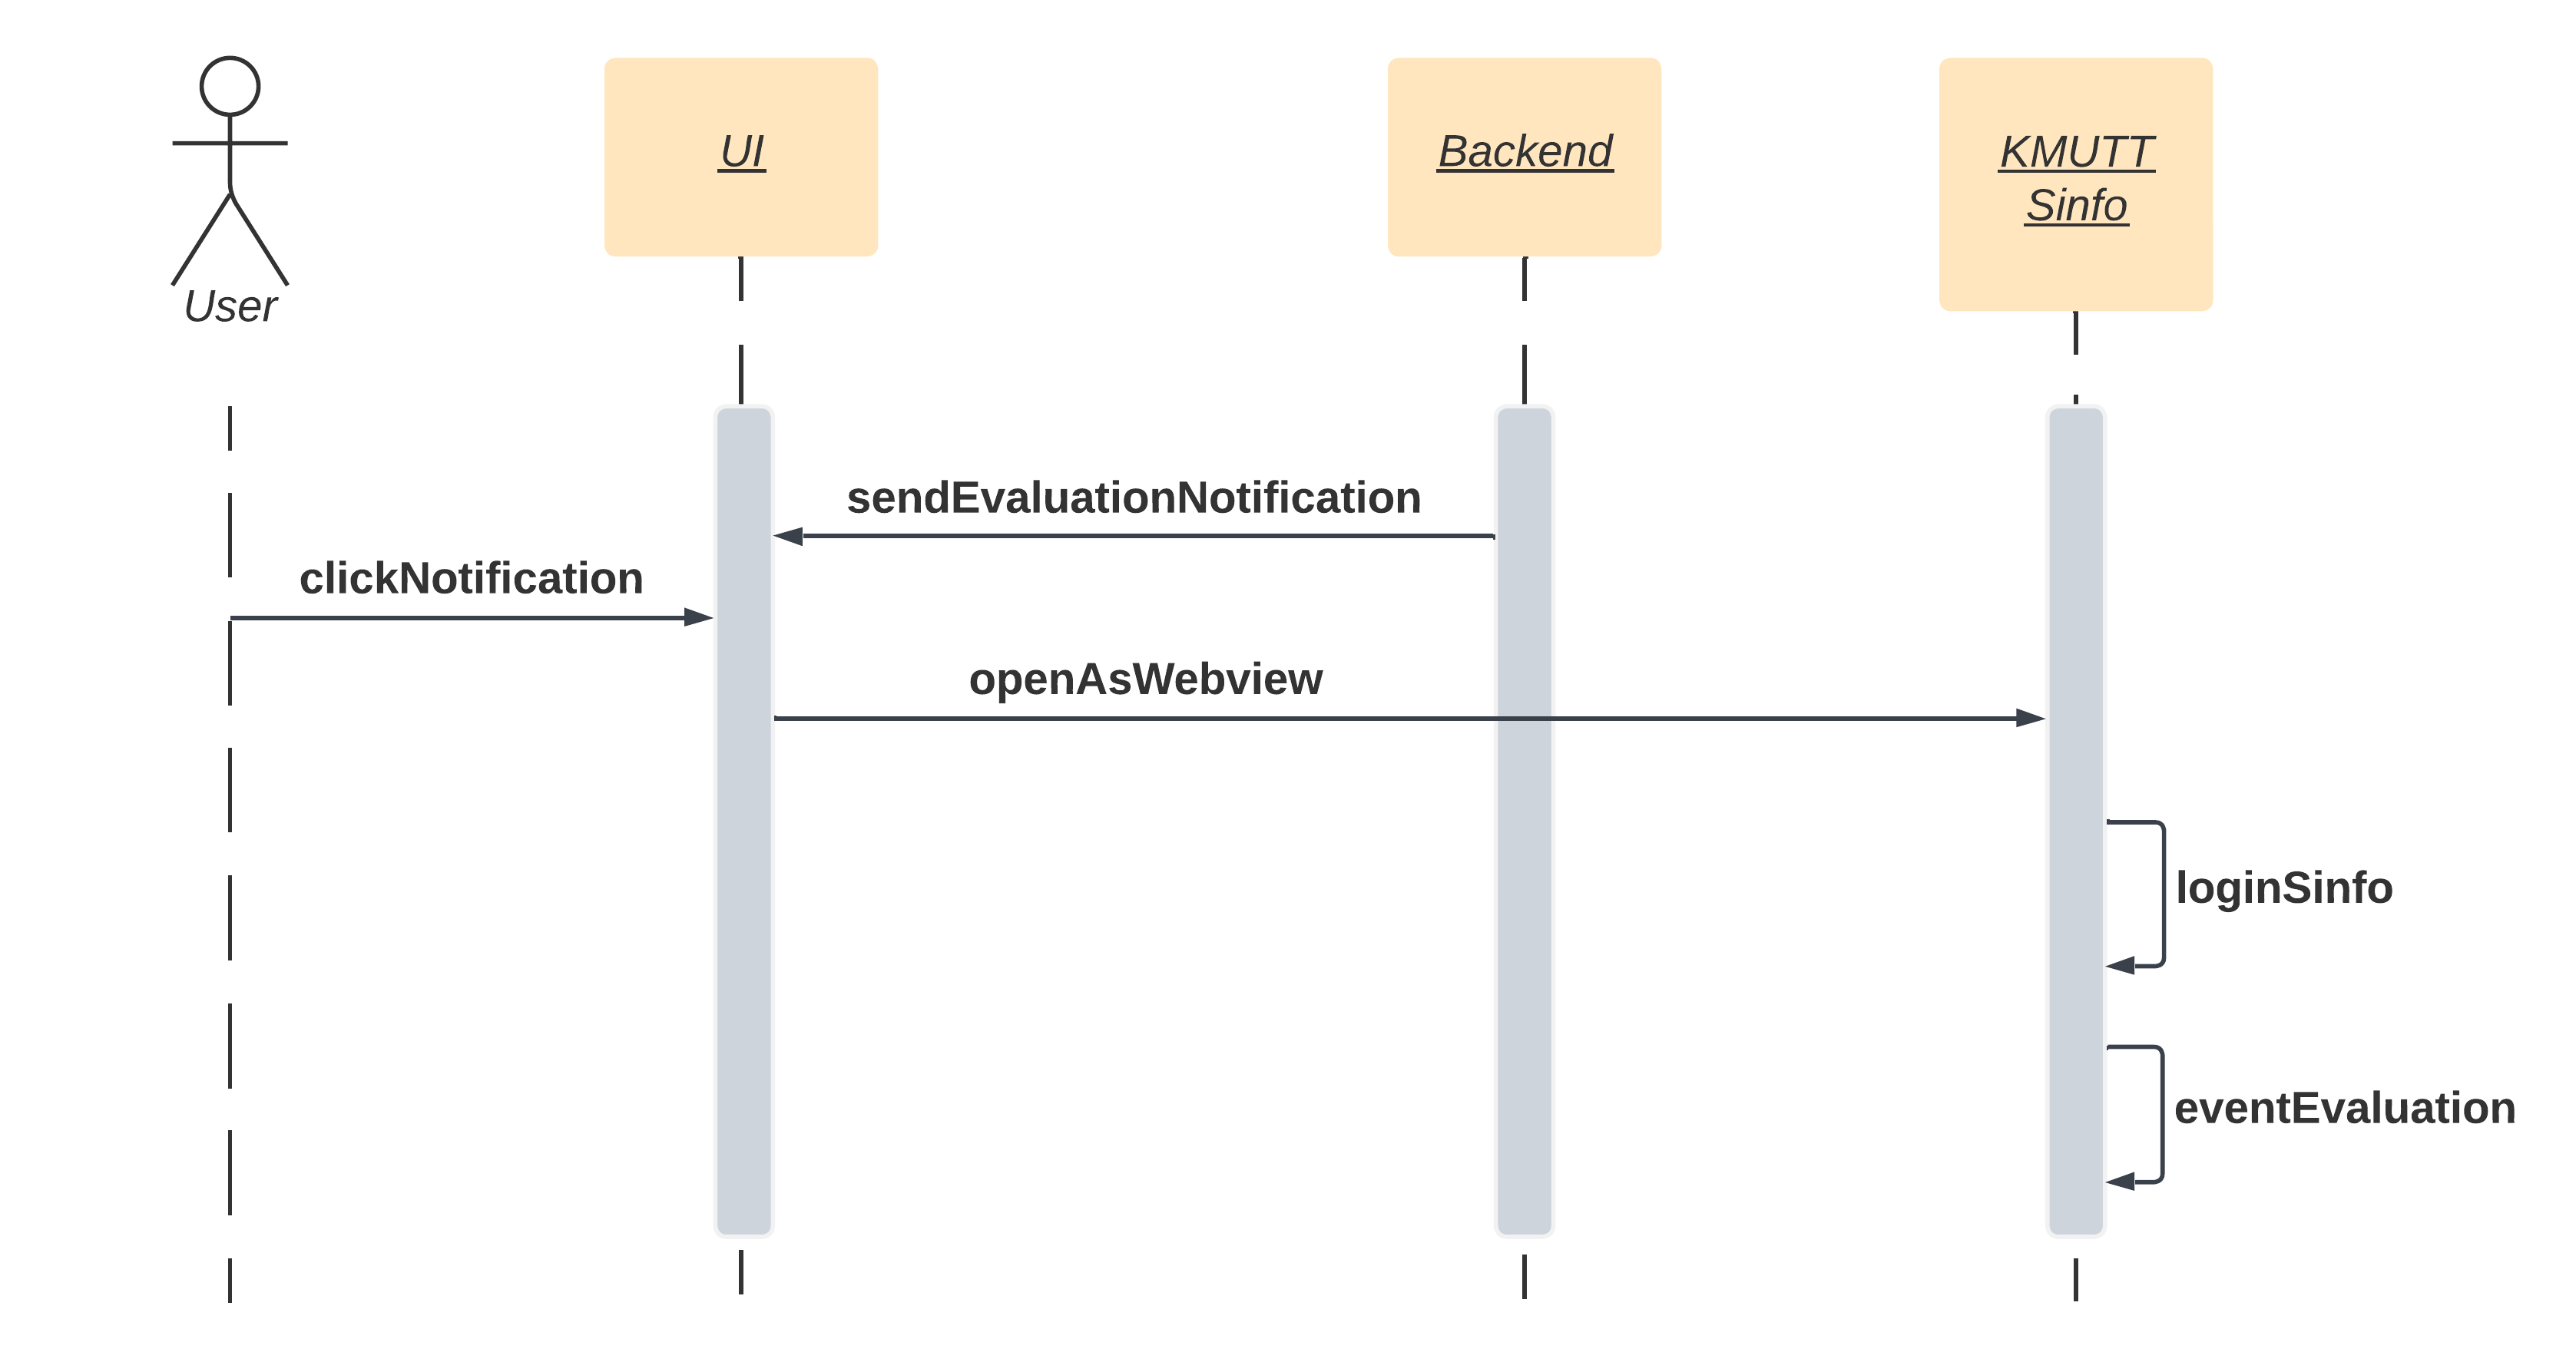
\includegraphics[width=13cm]{./Pictures/evaluate.png}}
    \caption{การประเมินกิจกรรม}\label{fig:Event evaluation}
  \end{figure}

  จากภาพ Sequence Diagram ในรูปที่ \ref{fig:Event evaluation} แสดงขั้นตอนการทำงานของระบบแจ้งเตือนการประเมินกิจกรรม โดยมีรายละเอียดดังนี้
  \begin{enumerate}
    \item Backend System จะตรวจสอบกำหนดการหรือเงื่อนไขที่ต้องแจ้งเตือนการประเมินกิจกรรมให้กับผู้ใช้งาน เช่น หลังจากกิจกรรมสิ้นสุดลงภายในระยะเวลาที่กำหนด
    \item เมื่อถึงกำหนดการหรือเงื่อนไขที่ต้องแจ้งเตือน Backend System จะส่งคำเตือนการประเมินกิจกรรมไปยัง User Interface (UI) ของผู้ใช้งาน
    \item UI จะแสดงข้อความแจ้งเตือนการประเมินกิจกรรมให้ผู้ใช้งานทราบ พร้อมกับลิงก์หรือปุ่มสำหรับเข้าไปประเมินกิจกรรม
    \item เมื่อผู้ใช้งานกดเข้าลิงก์หรือปุ่มประเมินกิจกรรม UI จะเปิดหน้าต่างหรือหน้าจอสำหรับให้ผู้ใช้งานประเมินกิจกรรมนั้น เพื่อให้ผู้ใช้งานกรอกข้อมูลและประเมินกิจกรรมลงในหน้าประเมินกิจกรรม
    \item หลังจากผู้ใช้งานกรอกข้อมูลการประเมินกิจกรรมเสร็จแล้ว UI จะส่งข้อมูลการประเมินดังกล่าวไปยัง Backend System และจะบันทึกข้อมูลการประเมินกิจกรรมของผู้ใช้งานลงใน Database
  \end{enumerate}
  โดยสรุป Sequence Diagram นี้แสดงให้เห็นถึงขั้นตอนการทำงานร่วมกันระหว่าง Backend System, User Interface และ Database ในการแจ้งเตือนให้ผู้ใช้งานประเมินกิจกรรม โดย Backend System จะเป็นผู้ส่งคำเตือนไปยัง UI เพื่อให้ UI แสดงข้อความแจ้งเตือนและลิงก์สำหรับเข้าประเมินกิจกรรมให้ผู้ใช้งาน หลังจากผู้ใช้งานประเมินกิจกรรมเสร็จแล้ว ข้อมูลการประเมินจะถูกส่งกลับไปบันทึกยัง Backend System และ Database

\newpage

\subsection{การแจ้งเตือนกิจกรรมชมรม}

  \begin{figure}[!h]\centering
    \setlength{\fboxrule}{0.5mm} % can define this in the preamble
    \setlength{\fboxsep}{0.5cm}
    \fbox{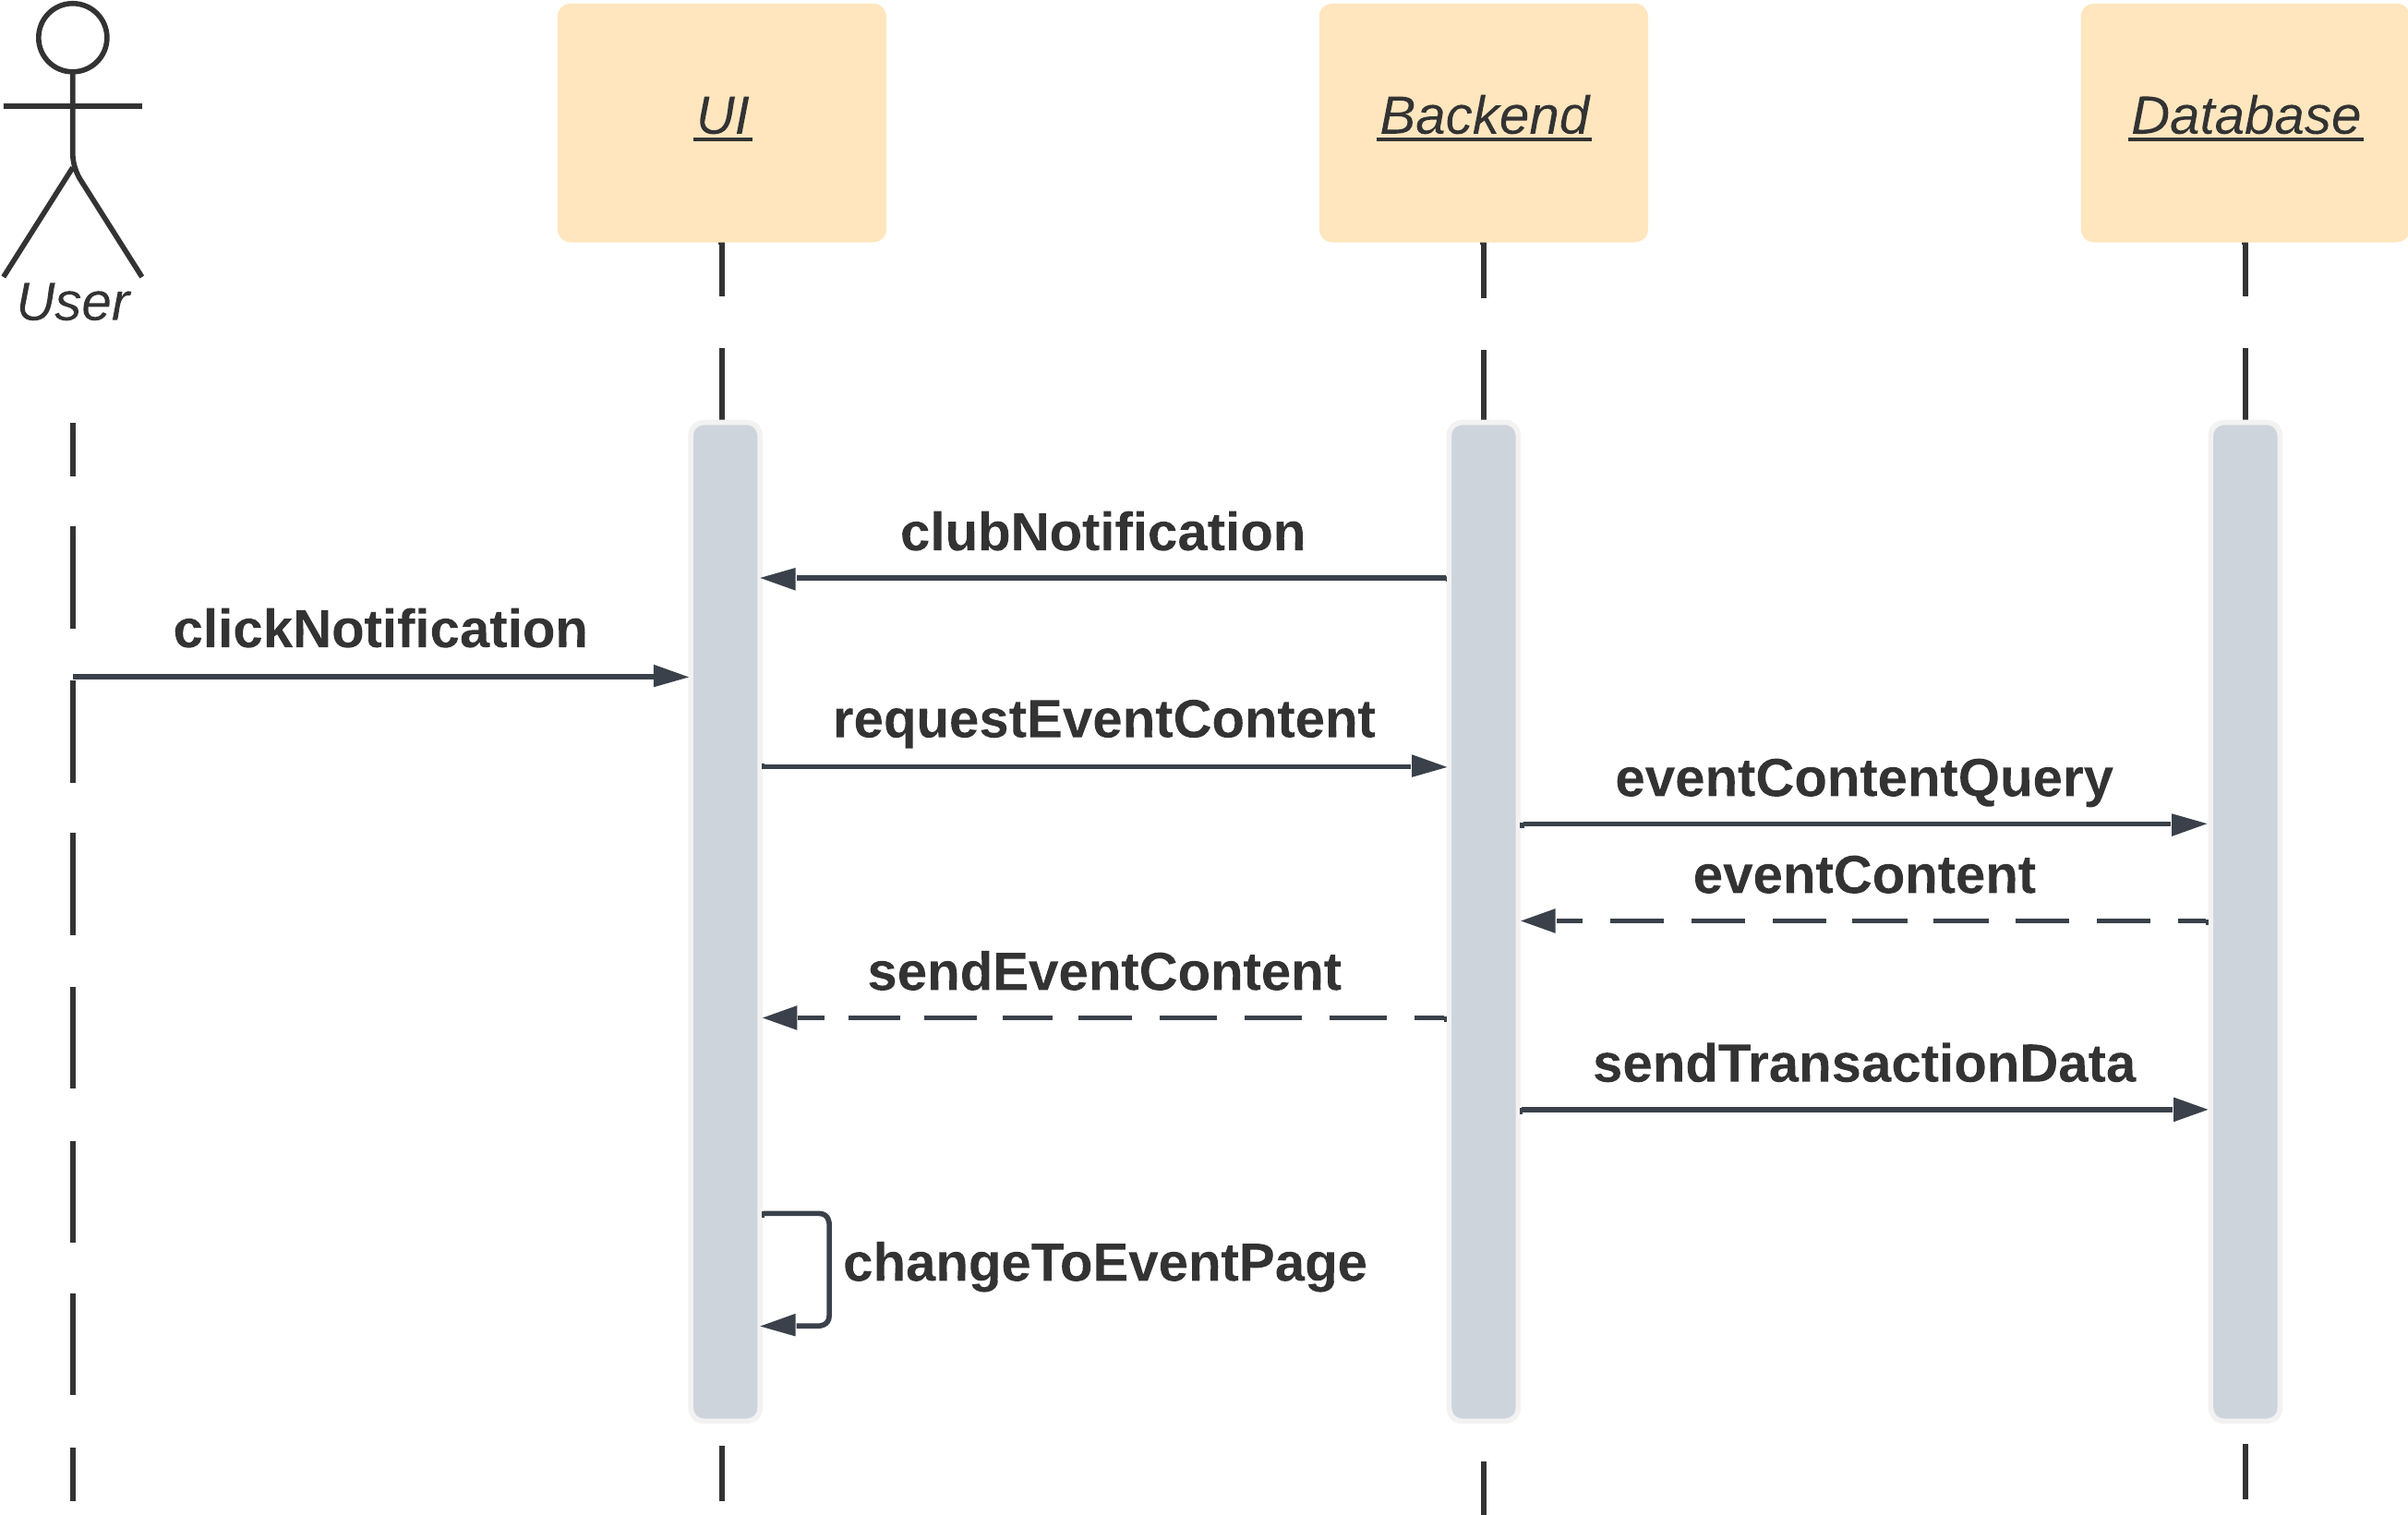
\includegraphics[width=12cm]{./Pictures/Noti.png}}
    \caption{การแจ้งเตือนกิจกรรมชมรม}\label{fig:Notification about event from club}
  \end{figure}

  จากภาพ Sequence Diagram ในรูปที่ \ref{fig:Notification about event from club} แสดงขั้นตอนการทำงานของระบบแจ้งเตือนกิจกรรมชมรม โดยมีรายละเอียดดังนี้
  \begin{enumerate}
    \item Backend System จะตรวจสอบกำหนดการหรือเงื่อนไขที่ต้องแจ้งเตือนกิจกรรมชมรมให้กับผู้ใช้งาน เช่น ก่อนถึงวันที่มีกิจกรรมชมรมตามระยะเวลาที่กำหนด
    \item เมื่อถึงกำหนดการหรือเงื่อนไขที่ต้องแจ้งเตือน Backend System จะส่งข้อความแจ้งเตือนกิจกรรมชมรมไปยัง User Interface (UI) ของผู้ใช้งาน
    \item UI จะแสดงข้อความแจ้งเตือนกิจกรรมชมรมให้ผู้ใช้งานทราบ พร้อมกับลิงก์หรือปุ่มสำหรับเข้าไปอ่านรายละเอียดของกิจกรรม
    \item เมื่อผู้ใช้งานกดเข้าลิงก์หรือปุ่มอ่านรายละเอียดกิจกรรม UI จะส่งคำขอไปยัง Backend System เพื่อให้ดึงข้อมูลรายละเอียดของกิจกรรมมาจาก Database
    \item Backend System จะค้นหาและดึงข้อมูลรายละเอียดของกิจกรรมที่ต้องการจาก Database
    \item Backend System จะส่งข้อมูลรายละเอียดของกิจกรรมกลับไปยัง UI
    \item UI จะแสดงข้อมูลรายละเอียดของกิจกรรมให้ผู้ใช้งานเห็น
    \item นอกจากนี้ Backend System จะบันทึกข้อมูลการใช้งานของผู้ใช้งาน เช่น การเข้าอ่านรายละเอียดกิจกรรม ลงใน Database ด้วย
  \end{enumerate}
  โดยสรุป Sequence Diagram นี้แสดงให้เห็นถึงขั้นตอนการทำงานร่วมกันระหว่าง Backend System, User Interface และ Database ในการแจ้งเตือนกิจกรรมชมรมให้ผู้ใช้งาน โดย Backend System จะเป็นผู้ส่งข้อความแจ้งเตือนไปยัง UI เพื่อให้ UI แสดงข้อความแจ้งเตือนและลิงก์สำหรับเข้าอ่านรายละเอียดกิจกรรมให้ผู้ใช้งาน เมื่อผู้ใช้งานเข้าอ่านรายละเอียดกิจกรรม UI จะขอข้อมูลรายละเอียดจาก Backend System ซึ่งจะดึงมาจาก Database และข้อมูลการใช้งานของผู้ใช้งานจะถูกบันทึกลงใน Database ด้วย

  \newpage

\subsection{การค้นหาชมรม}

  \begin{figure}[!h]\centering
    \setlength{\fboxrule}{0.5mm} % can define this in the preamble
    \setlength{\fboxsep}{0.5cm}
    \fbox{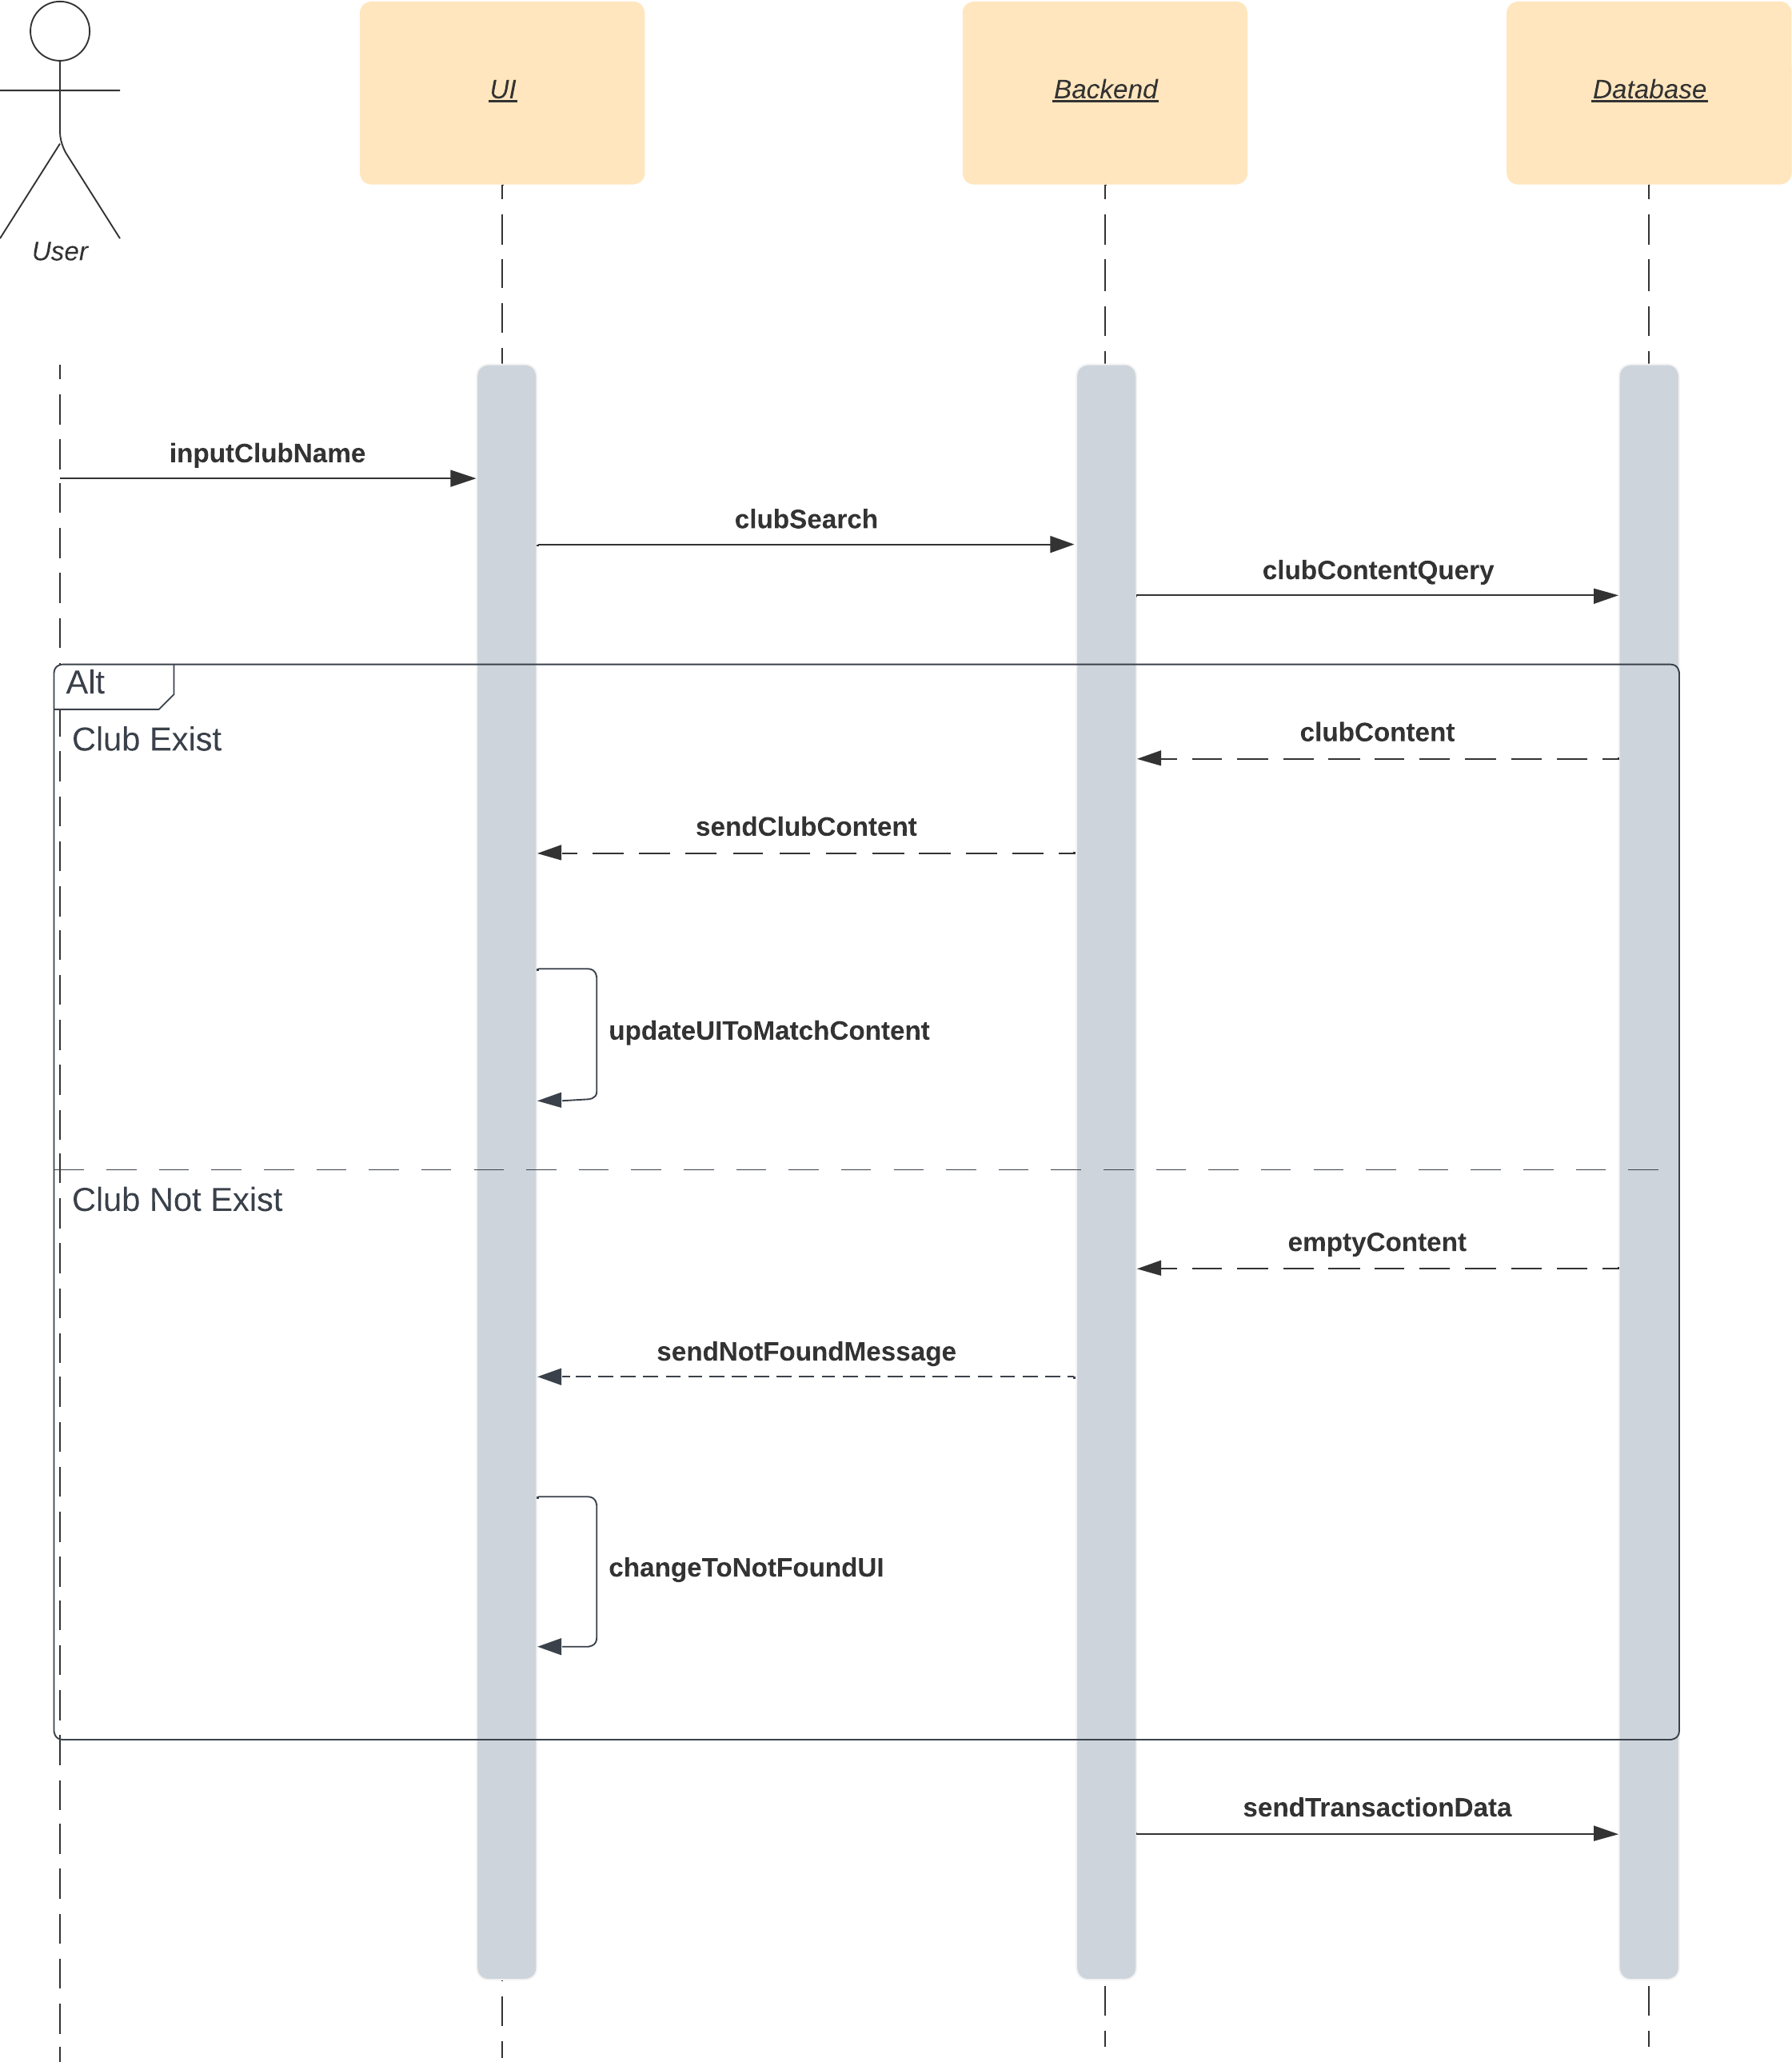
\includegraphics[width=11cm]{./Pictures/searchclub.png}}
    \caption{การค้นหาชมรม}\label{fig:Seacrh club}
  \end{figure}

  จากภาพ Sequence Diagram ในรูปที่ \ref{fig:Seacrh club} แสดงขั้นตอนการทำงานของระบบเมื่อผู้ใช้งานต้องการค้นหาชมรม โดยมีรายละเอียดดังนี้
  \begin{enumerate}
    \item ผู้ใช้งานเริ่มต้นโดยการป้อนคำค้นหาหรือเงื่อนไขที่ต้องการค้นหาชมรมลงในช่องค้นหาบนหน้า User Interface (UI) ของระบบ
    \item หลังจากผู้ใช้งานป้อนคำค้นหาเรียบร้อยแล้ว UI จะส่งคำค้นหาหรือเงื่อนไขดังกล่าวไปยัง Backend System
    \item Backend System จะทำการค้นหาข้อมูลชมรมที่ตรงกับคำค้นหาหรือเงื่อนไขที่ได้รับมาจาก Database
    \item หากพบข้อมูลชมรมที่ตรงกับคำค้นหาหรือเงื่อนไข Backend System จะส่งข้อมูลชมรมเหล่านั้นกลับไปยัง UI
    \item UI จะแสดงข้อมูลชมรมที่ค้นหาได้ให้ผู้ใช้งานเห็น
    \item หากไม่พบข้อมูลชมรมที่ตรงกับคำค้นหาหรือเงื่อนไข Backend System จะแจ้งกลับไปยัง UI ว่าไม่พบข้อมูลชมรมที่ค้นหา
    \item UI จะแสดงข้อความ "ไม่พบชมรมที่ค้นหา" ให้ผู้ใช้งานทราบ
    \item นอกจากนี้ Backend System จะบันทึกข้อมูลการค้นหาชมรมของผู้ใช้งานลงใน Database ด้วย ไม่ว่าการค้นหานั้นจะประสบความสำเร็จหรือไม่ก็ตาม
  \end{enumerate}

  โดยสรุป Sequence Diagram นี้แสดงให้เห็นถึงขั้นตอนการทำงานร่วมกันระหว่าง User Interface, Backend System และ Database ในการค้นหาข้อมูลชมรมตามคำค้นหาหรือเงื่อนไขที่ผู้ใช้งานต้องการ โดยจะแสดงผลการค้นหาให้ผู้ใช้งานทราบ และบันทึกข้อมูลการค้นหาลงใน Database ไม่ว่าผลการค้นหาจะสำเร็จหรือไม่ก็ตาม

  \newpage

\subsection{อ่านรายละเอียดของชมรมและการเข้าร่วมชมรม}

  \begin{figure}[!h]\centering
    \setlength{\fboxrule}{0.5mm} % can define this in the preamble
    \setlength{\fboxsep}{0.5cm}
    \fbox{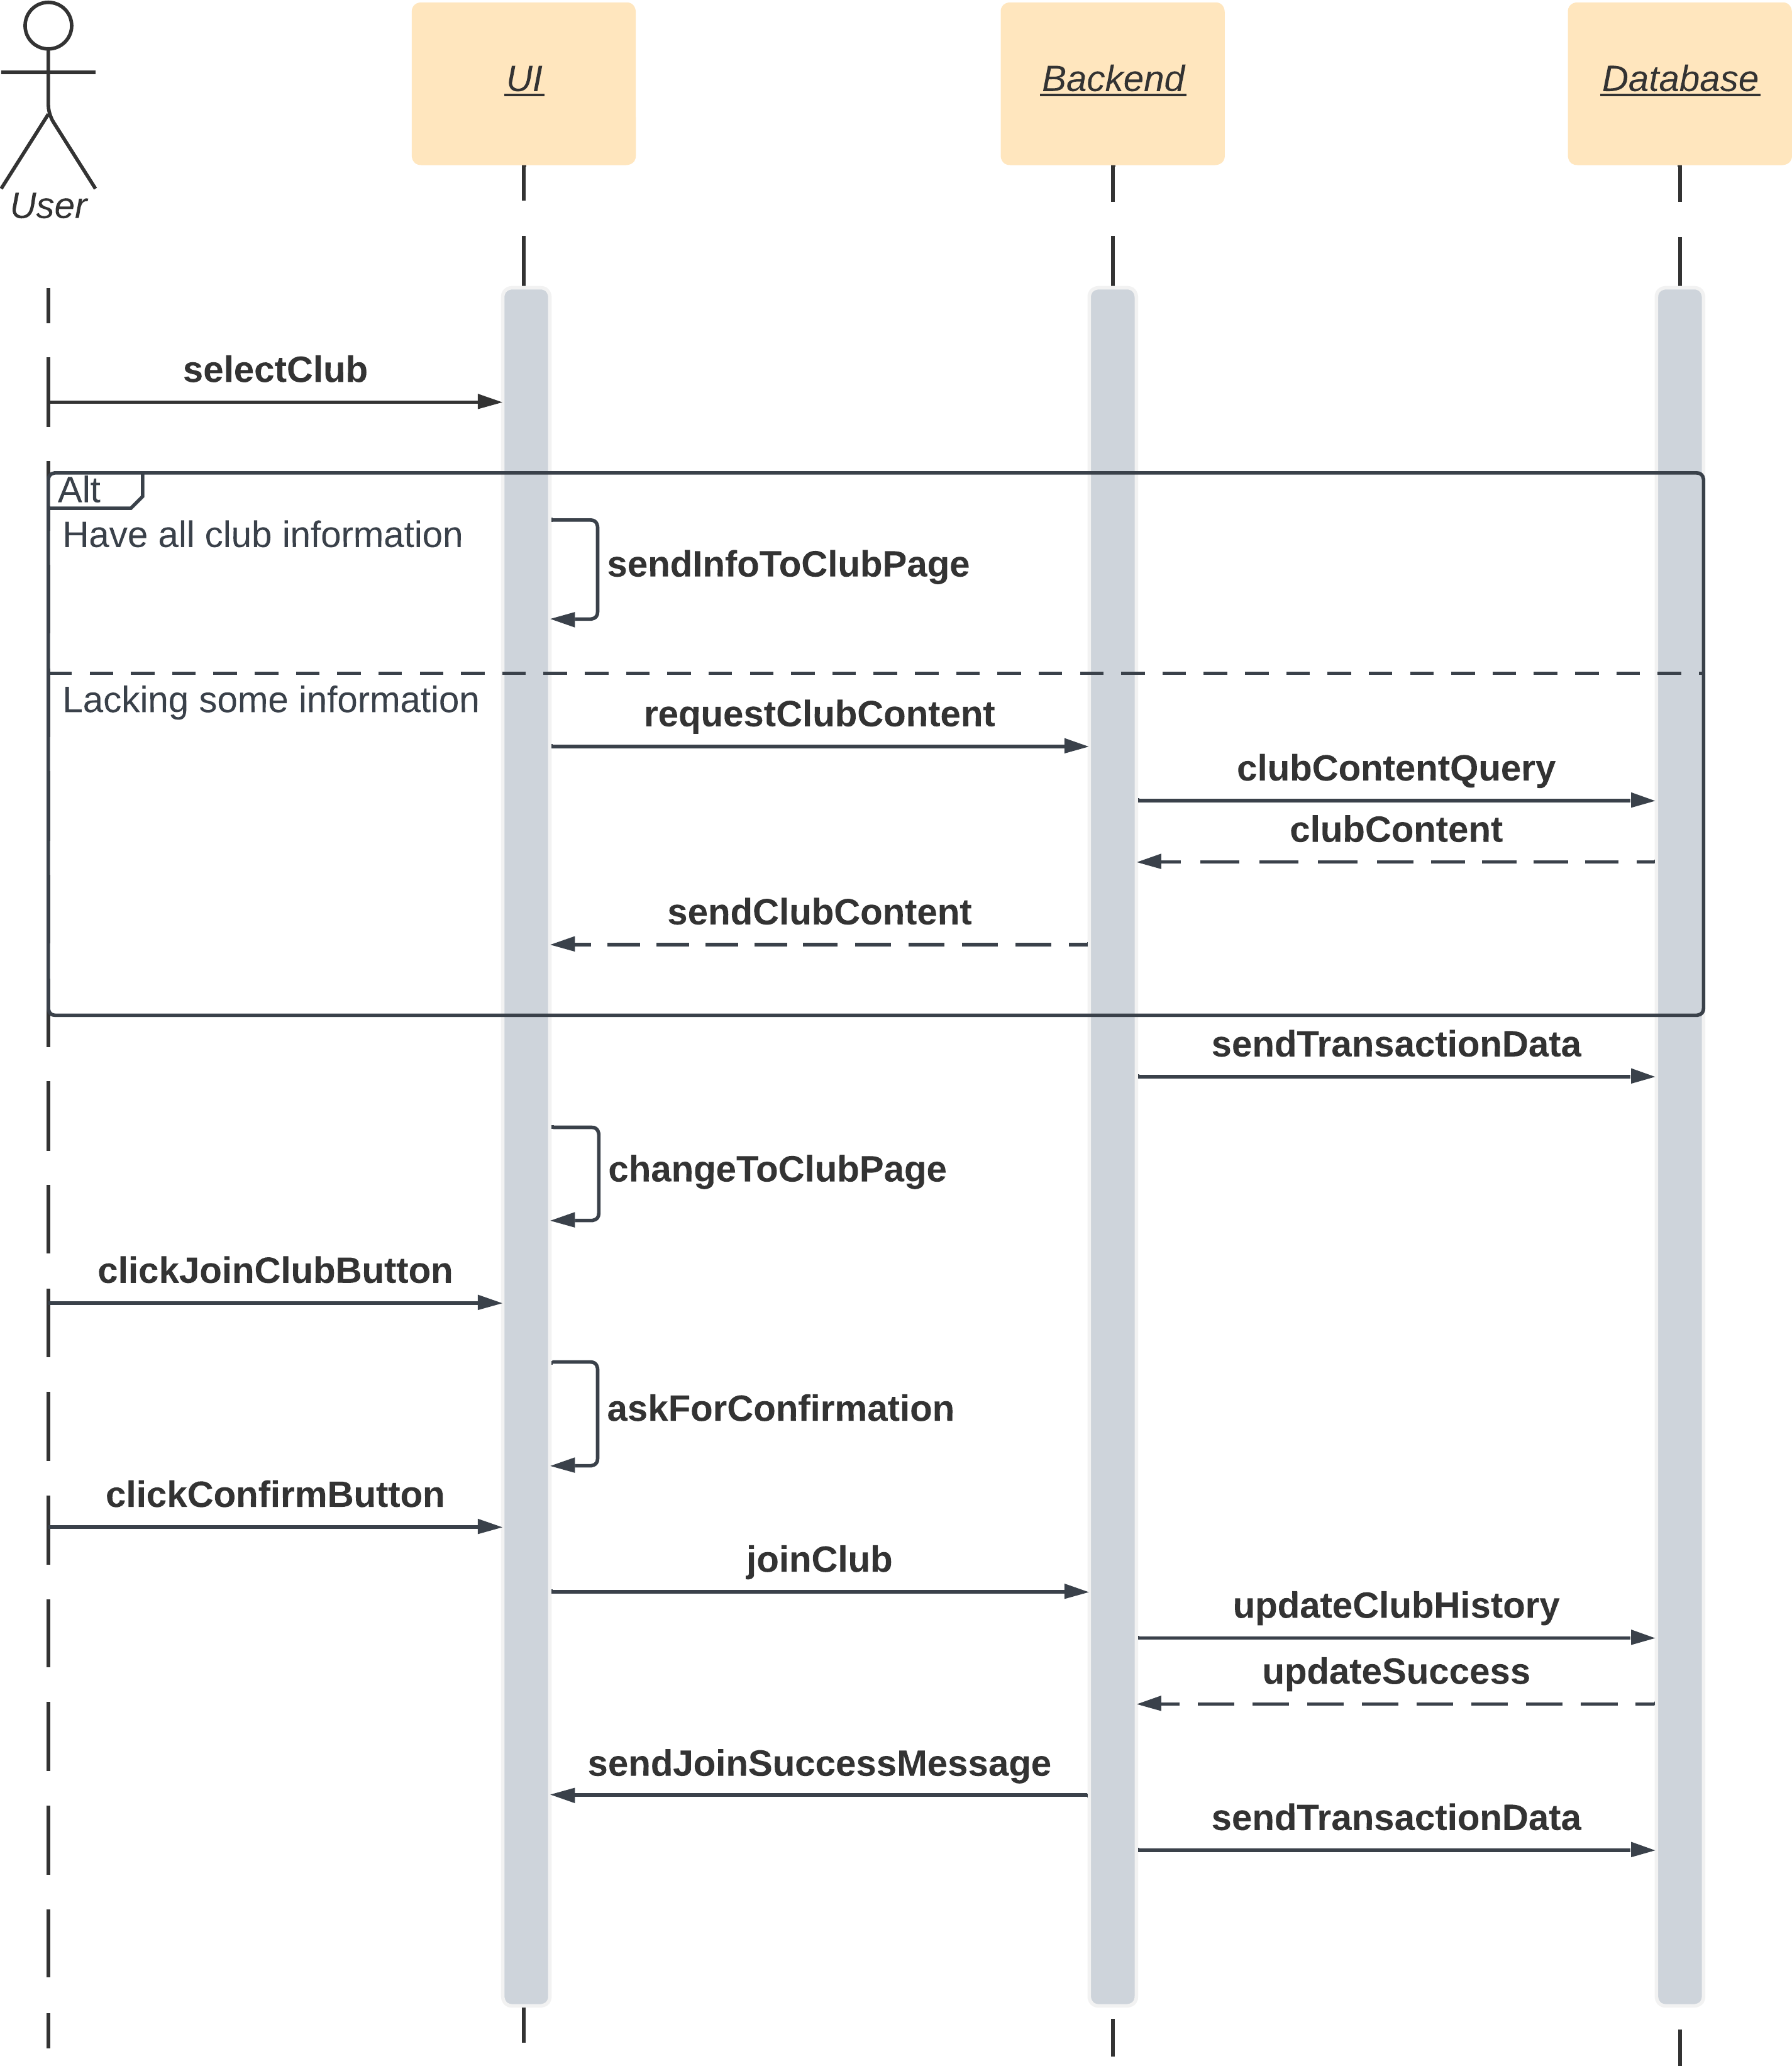
\includegraphics[width=10cm]{./Pictures/selectandjoinclub.png}}
    \caption{อ่านรายละเอียดของชมรมและการเข้าร่วมชมรม}\label{fig:Select and join club}
  \end{figure}

  จากภาพ Sequence Diagram ในรูปที่ \ref{fig:Select and join club} แสดงขั้นตอนการทำงานของระบบเมื่อผู้ใช้งานต้องการอ่านรายละเอียดของชมรม และเข้าร่วมชมรมนั้น โดยมีรายละเอียดดังนี้
  \begin{enumerate}
    \item ผู้ใช้งานเลือกชมรมที่ต้องการอ่านรายละเอียดจากหน้า User Interface (UI) ของระบบ
    \item UI จะตรวจสอบว่ามีข้อมูลรายละเอียดของชมรมดังกล่าวอยู่ในระบบหรือไม่ และจะแสดงข้อมูลรายละเอียดนั้นให้ผู้ใช้งานเห็น
    \item หากไม่มีข้อมูลรายละเอียดของชมรม UI จะส่งคำขอไปยัง Backend System เพื่อให้ดึงข้อมูลรายละเอียดของชมรมมาจาก Database
    \item Backend System จะค้นหาและดึงข้อมูลรายละเอียดของชมรมที่ต้องการจาก Database และส่งไปยัง UI และแสดงให้ผู้ใช้งานเห็น
    \item หากผู้ใช้งานต้องการเข้าร่วมชมรมนั้น ผู้ใช้งานจะกดปุ่มเข้าร่วมชมรมบนหน้า UI และจะแสดงข้อความยืนยันการเข้าร่วมชมรมให้ผู้ใช้งาน
    \item หากผู้ใช้งานยืนยันการเข้าร่วมชมรม UI จะส่งข้อมูลการเข้าร่วมชมรมของผู้ใช้งานไปยัง Backend System
    \item Backend System จะบันทึกข้อมูลการเข้าร่วมชมรมของผู้ใช้งานลงใน Database
  \end{enumerate}

  โดยสรุป Sequence Diagram นี้แสดงให้เห็นถึงขั้นตอนการทำงานร่วมกันระหว่าง User Interface, Backend System และ Database ในการแสดงรายละเอียดของชมรมให้ผู้ใช้งาน และรับข้อมูลการเข้าร่วมชมรมจากผู้ใช้งาน โดยมีการยืนยันการเข้าร่วมชมรมจากผู้ใช้งานก่อน เพื่อป้องกันการเข้าร่วมชมรมโดยไม่ได้ตั้งใจ


\subsection{การลาออกจากชมรม}

  \begin{figure}[!h]\centering
    \setlength{\fboxrule}{0.5mm} % can define this in the preamble
    \setlength{\fboxsep}{0.5cm}
    \fbox{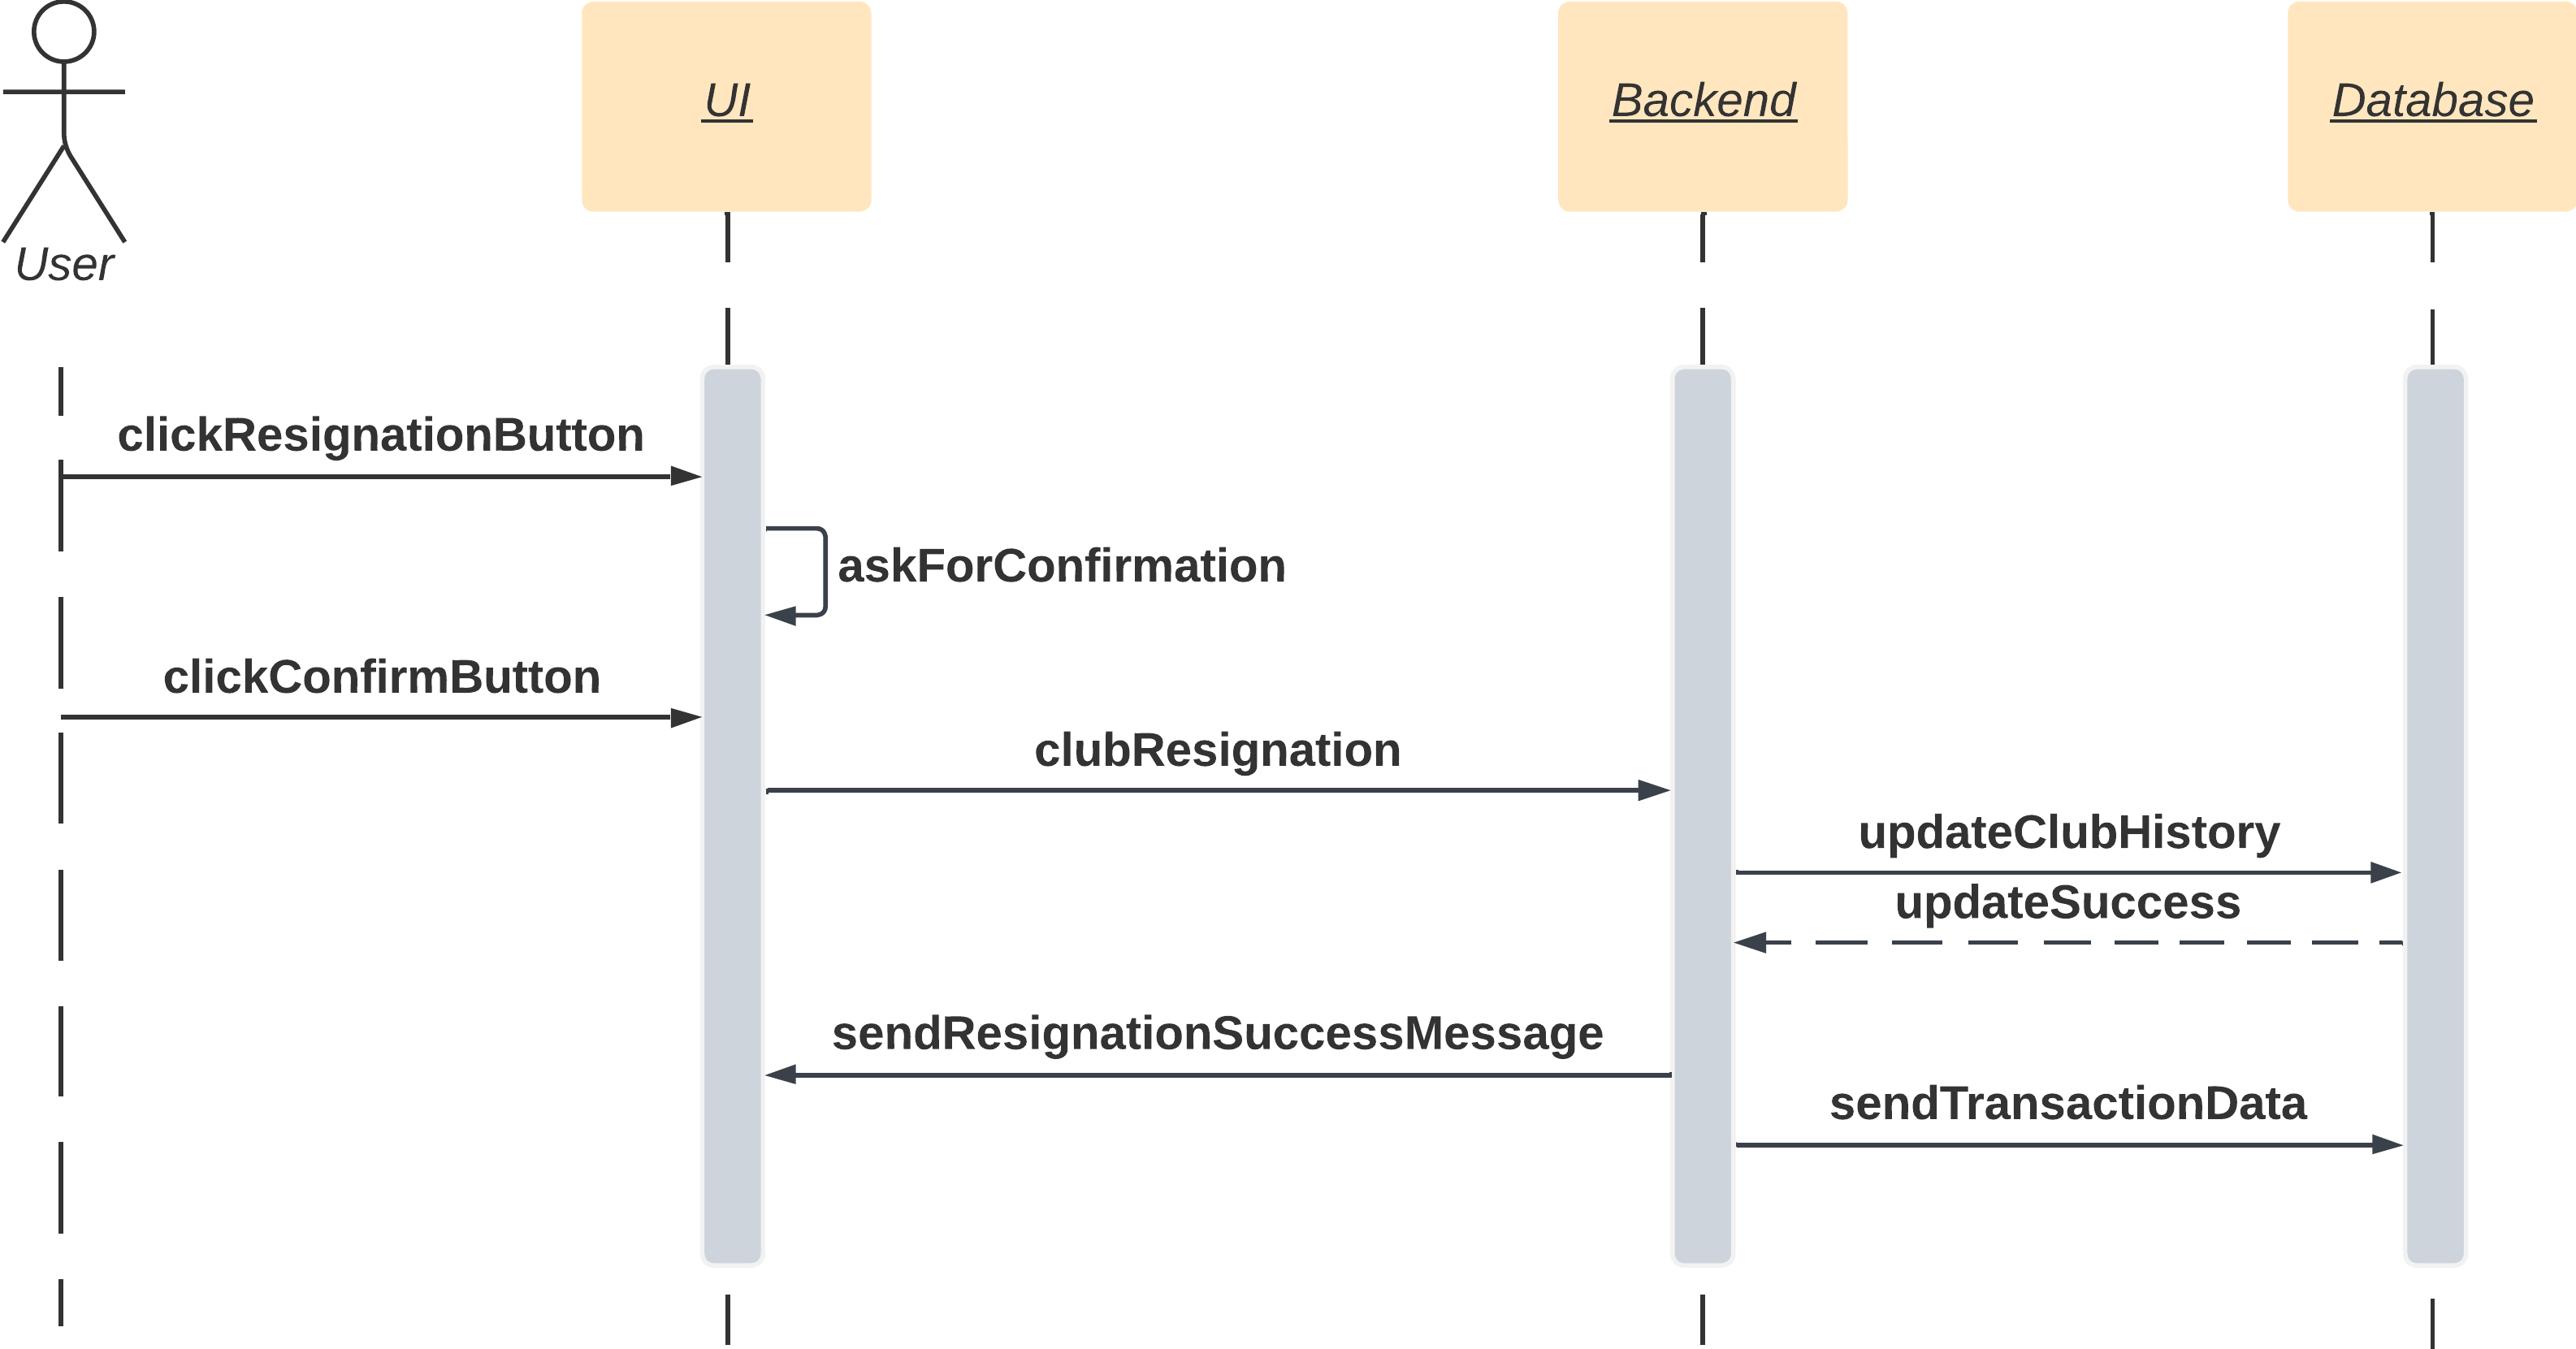
\includegraphics[width=13cm]{./Pictures/clubresign.png}}
    \caption{การลาออกจากชมรม}\label{fig:Club resignation}
  \end{figure}

  จากภาพ Sequence diagram ในรูปที่ \ref{fig:Club resignation} ซึ่งแสดงการทำงานของระบบขณะที่ผู้ใช้งานทำการลาออกจากชมรม ดังนี้
  \begin{enumerate}
    \item เริ่มต้นเมื่อผู้ใช้งานกดปุ่มลาออกจากส่วนติดต่อผู้ใช้ (UI)
    \item UI จะแสดงข้อความถามยืนยันการลาออกจากชมรมให้ผู้ใช้งาน
    \item หากผู้ใช้งานยืนยันการลาออก UI จะส่งข้อมูลการร้องขอลาออกไปยัง Backend
    \item Backend จะประมวลผลข้อมูลการลาออกและบันทึกลงในฐานข้อมูล (Database)
    \item หลังจากบันทึกข้อมูลเรียบร้อยแล้ว Backend จะส่งข้อความยืนยันการลาออกกลับไปที่ UI
    \item UI จะแสดงข้อความยืนยันการลาออกให้ผู้ใช้งานทราบ
  \end{enumerate}
  โดยสรุป Sequence diagram นี้แสดงถึงขั้นตอนการทำงานระหว่างส่วนติดต่อผู้ใช้ (UI) กับระบบหลังบ้าน (Backend) และฐานข้อมูล (Database) ในกระบวนการลาออกจากชมรมของผู้ใช้งาน ซึ่งประกอบด้วยการยืนยันจากผู้ใช้งาน การประมวลผลและบันทึกข้อมูลจาก Backend และการแสดงผลข้อความยืนยันจาก UI

  \newpage

\subsection{การแนะนำกิจกรรมให้ผู้ใช้งาน}

  \begin{figure}[!h]\centering
    \setlength{\fboxrule}{0.5mm} % can define this in the preamble
    \setlength{\fboxsep}{0.5cm}
    \fbox{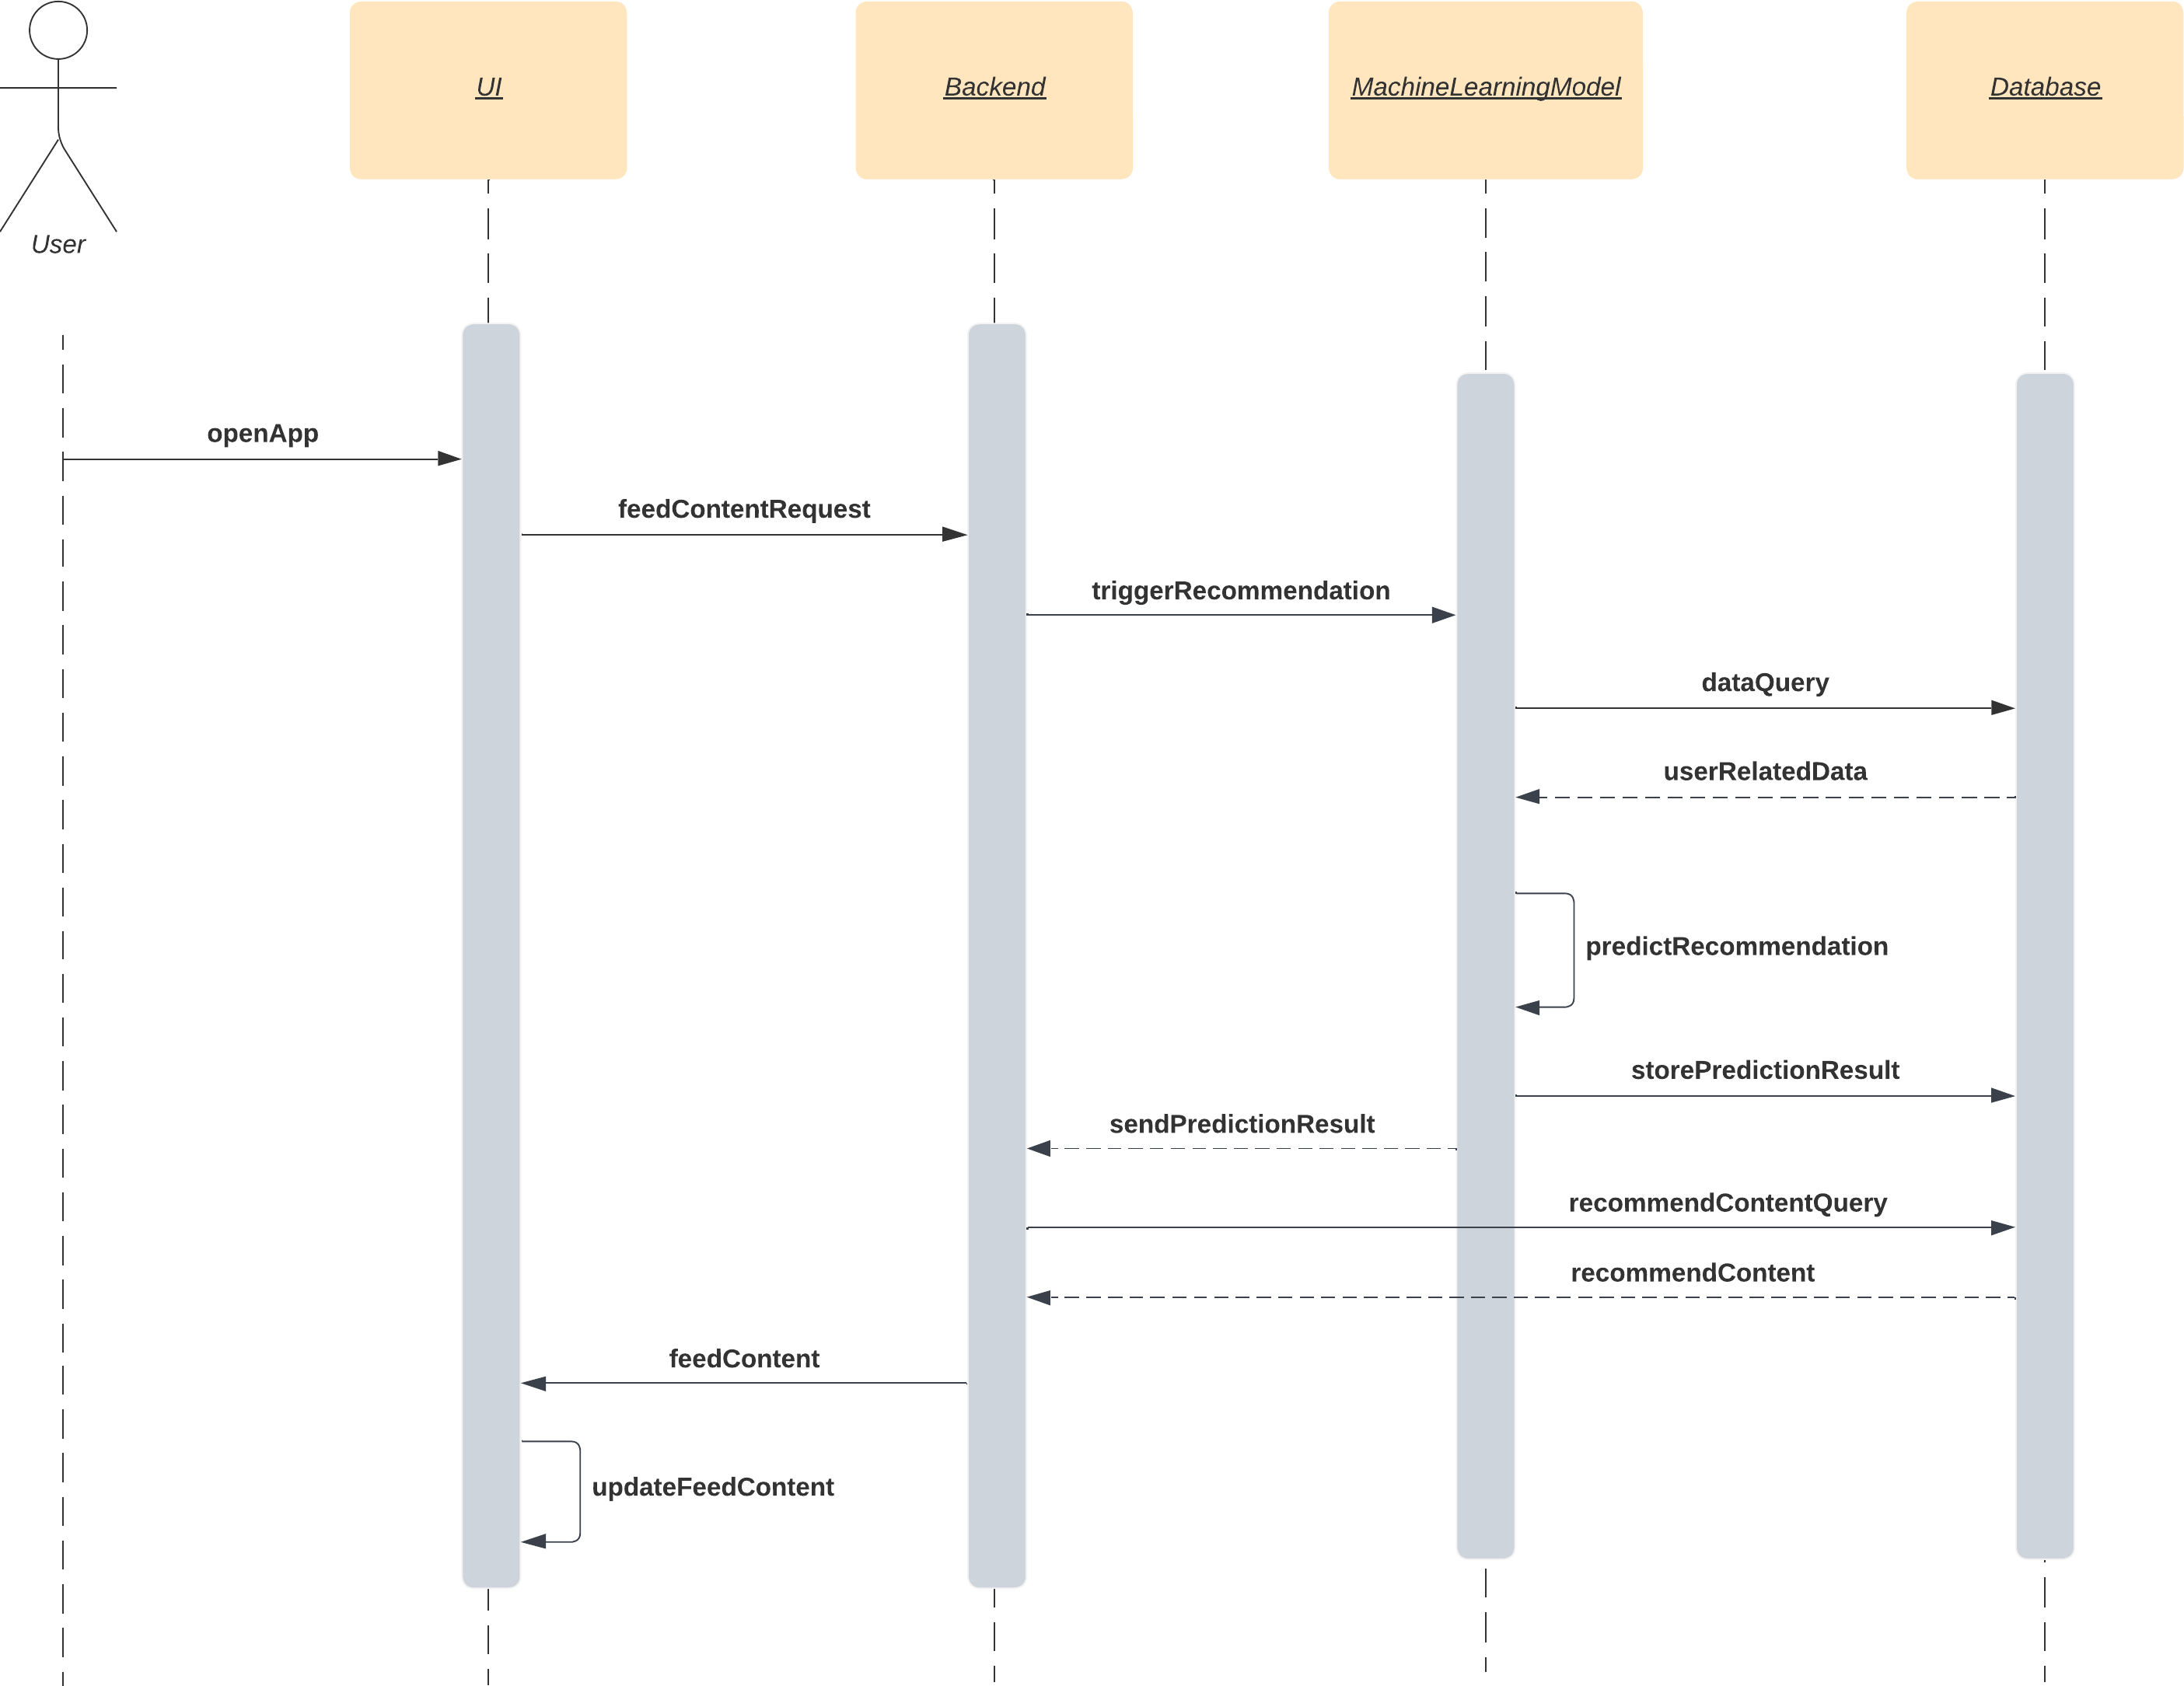
\includegraphics[width=12cm]{./Pictures/Recommend.png}}
    \caption{การแนะนำกิจกรรมให้ผู้ใช้งาน}\label{fig:Feed recommendation}
  \end{figure}

  จากภาพ Sequence diagram ในรูปที่ \ref{fig:Feed recommendation} ซึึ่งแสดงการทำงานของระบบในการแนะนำกิจกรรมให้แก่ผู้ใช้งาน ดังนี้
  \begin{enumerate}
    \item เริ่มต้นเมื่อผู้ใช้งานเปิดแอปพลิเคชันบนส่วนติดต่อผู้ใช้ (UI)
    \item UI จะส่งคำร้องขอเนื้อหาเพื่อแนะนำกิจกรรมไปยังระบบหลังบ้าน (Backend)
    \item Backend จะส่งคำร้องขอไปยังระบบ Machine Learning Model เพื่อประมวลผลคำแนะนำกิจกรรม
    \item Machine Learning Model จะดึงข้อมูลประวัติและพฤติกรรมของผู้ใช้งานจากฐานข้อมูล (Database) มาประมวลผล
    \item หลังประมวลผลเสร็จ Machine Learning Model จะส่งคำแนะนำกิจกรรมกลับไปที่ Backend
    \item Backend จะส่งคำแนะนำกิจกรรมไปแสดงบนส่วนติดต่อผู้ใช้ (UI) ให้ผู้ใช้งานเห็น
    \item พร้อมกันนี้ Backend จะบันทึกคำแนะนำกิจกรรมลงในฐานข้อมูล (Database) เพื่อใช้ในการประมวลผลครั้งต่อไป \\
    นอกจากนี้ เมื่อผู้ใช้งานต้องการดูคำแนะนำกิจกรรมย้อนหลัง สามารถทำได้โดย
    \item UI ส่งคำร้องขอดูประวัติคำแนะนำไปยัง Backend
    \item Backend ดึงข้อมูลคำแนะนำกิจกรรมย้อนหลังจากฐานข้อมูล (Database)
    \item Backend ส่งคำแนะนำกิจกรรมย้อนหลังไปแสดงบน UI ให้ผู้ใช้งานเห็น
  \end{enumerate}
  โดยสรุป Sequence diagram นี้แสดงถึงการทำงานร่วมกันของ UI, Backend, Machine Learning Model และ Database ในการแนะนำกิจกรรมให้แก่ผู้ใช้งานตามประวัติและพฤติกรรม รวมถึงการบันทึกและแสดงประวัติคำแนะนำย้อนหลัง

\newpage

\subsection{การ Train Model การเรียนรู้ของเครื่อง}

  \begin{figure}[!h]\centering
    \setlength{\fboxrule}{0.5mm} % can define this in the preamble
    \setlength{\fboxsep}{0.5cm}
    \fbox{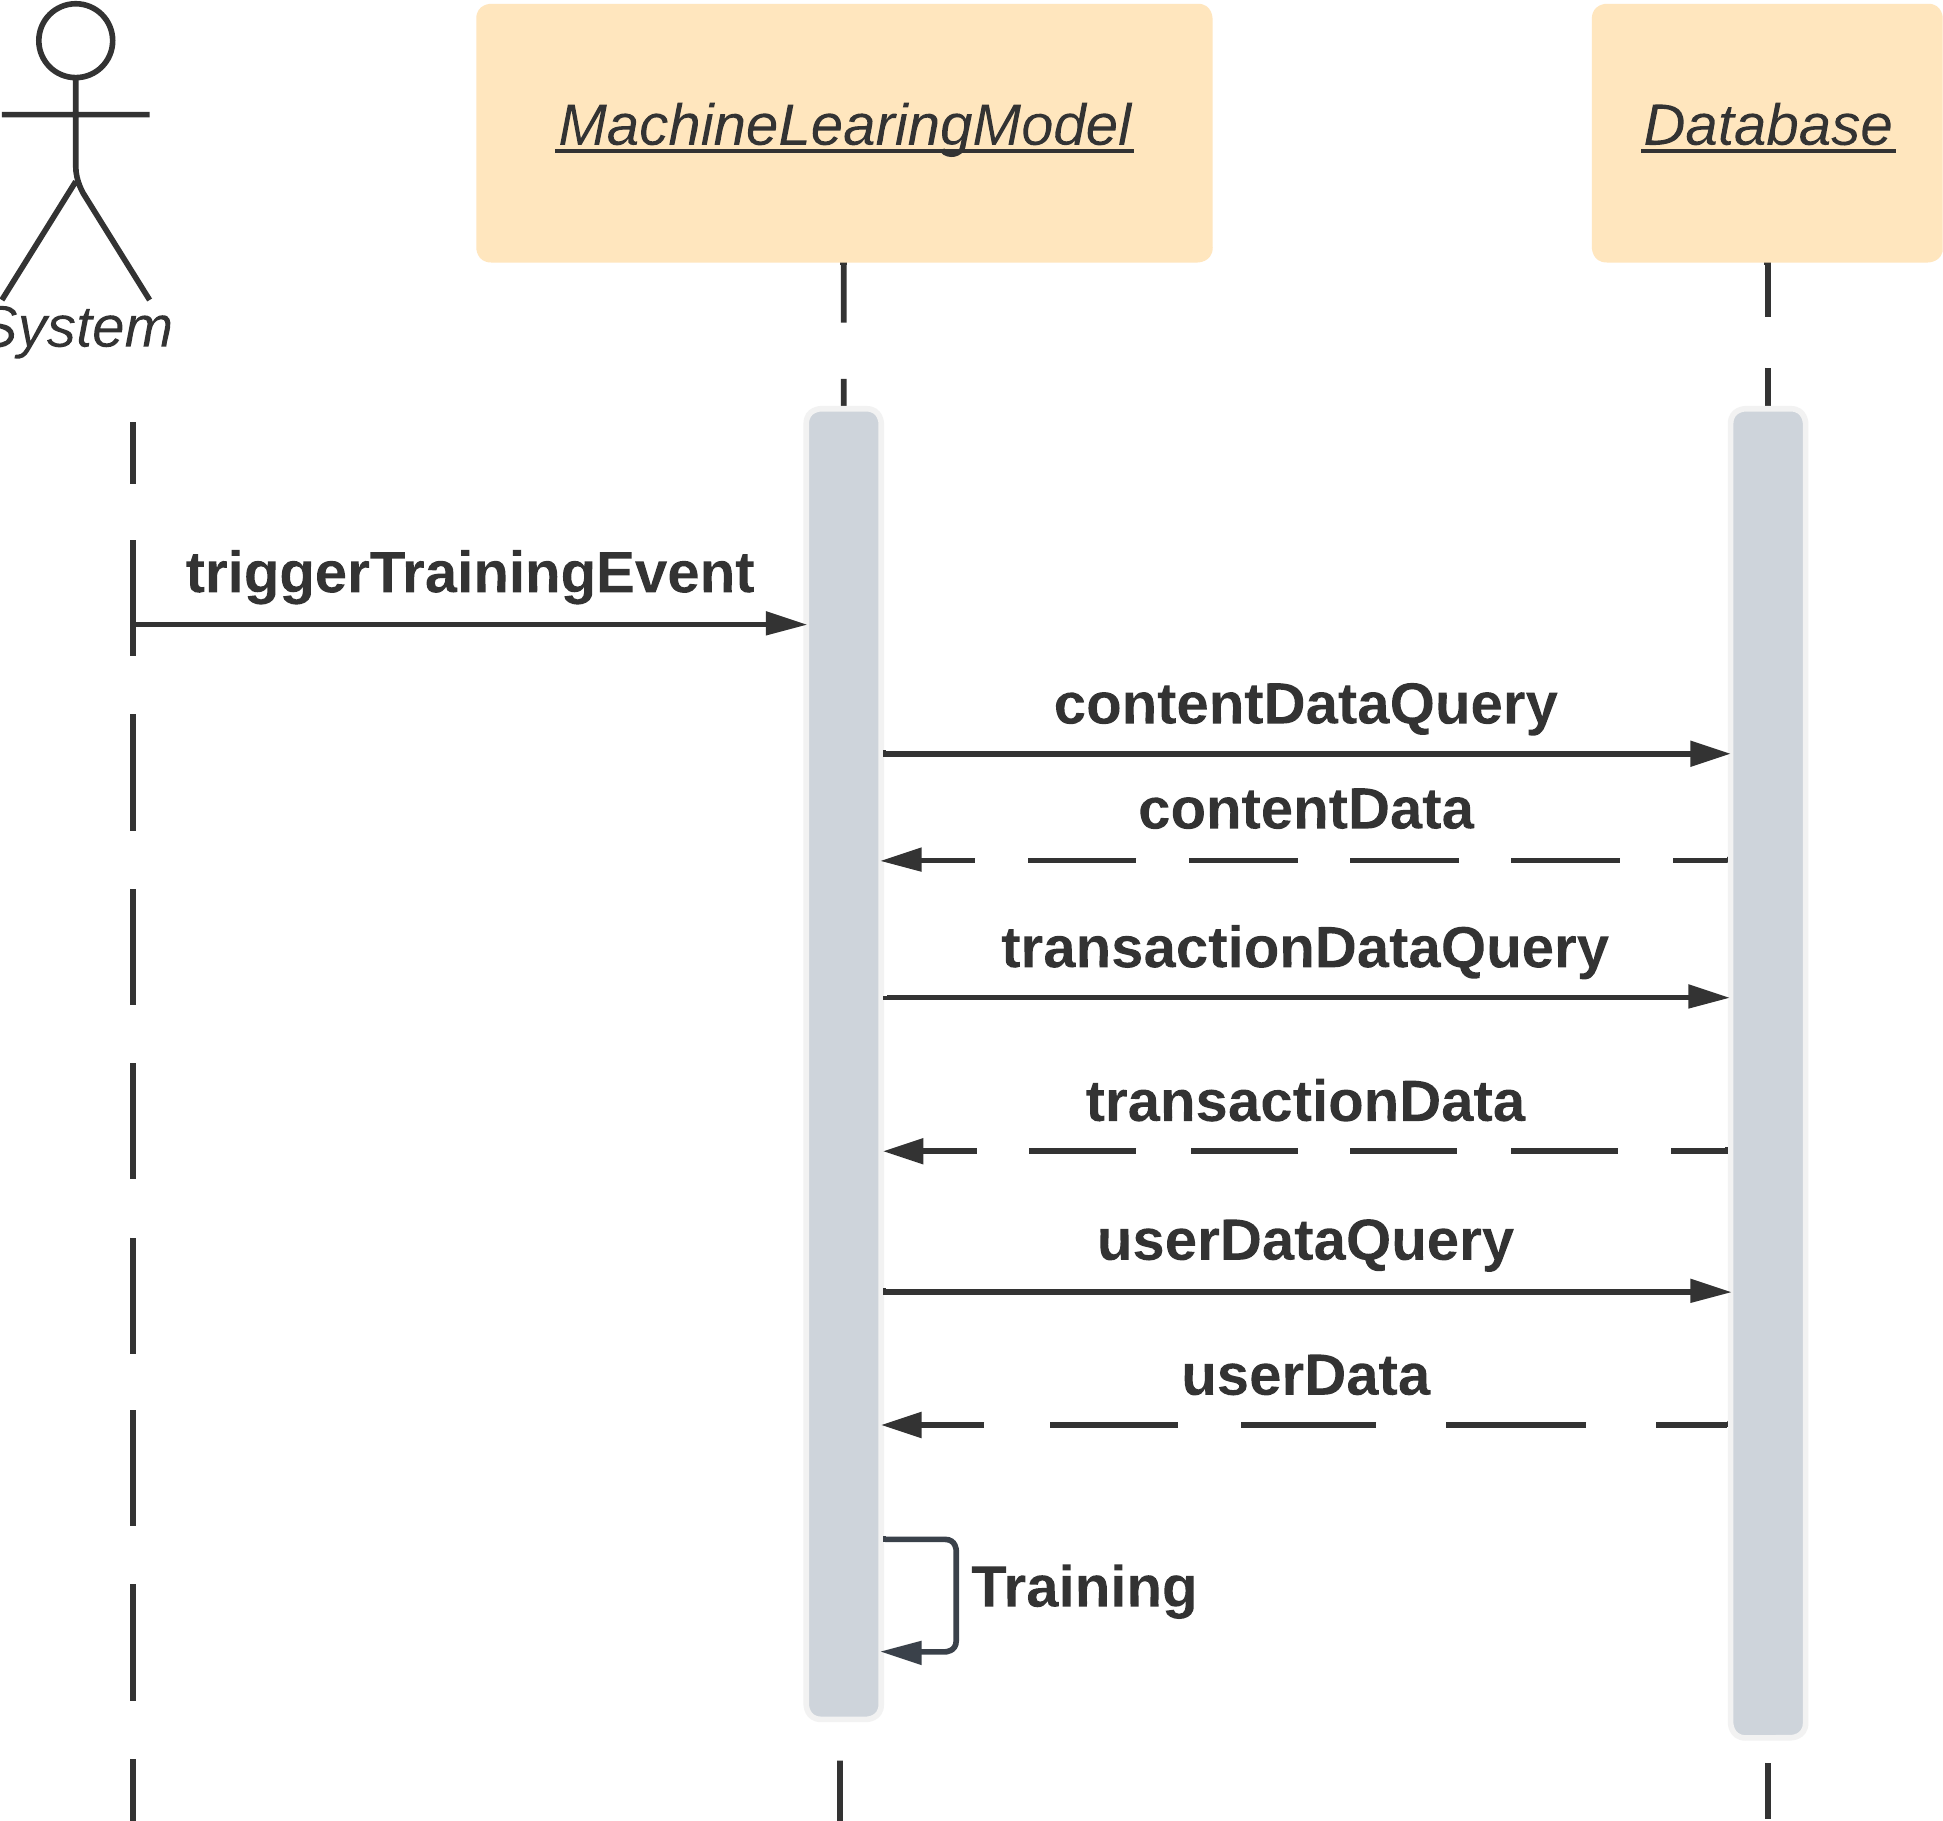
\includegraphics[width=12cm]{./Pictures/Machinelearning.png}}
    \caption{การ Train Model การเรียนรู้ของเครื่อง}\label{fig:Machine learning training}
  \end{figure}
  
  จากภาพ Sequence Diagram ในรูปที่ \ref{fig:Machine learning training} ซึ่งแสดงการทำงานของระบบในขณะที่มีการ Train Model การเรียนรู้ของเครื่องใหม่ สามารถขยายความได้ดังนี้
  \begin{enumerate}
    \item เริ่มต้นเมื่อระบบต้องการทำการ Train หรือปรับปรุงประสิทธิภาพของ Machine Learning Model
    \item Machine Learning Model จะส่งคำร้องขอข้อมูลกิจกรรมและการใช้งานของผู้ใช้ไปยังฐานข้อมูล (Database)
    \item ฐานข้อมูลจะรวบรวมและส่งข้อมูลที่เกี่ยวข้อง ได้แก่ ข้อมูลกิจกรรม พฤติกรรมการใช้งาน ฯลฯ ไปให้ Machine Learning Model
    \item Machine Learning Model จะนำข้อมูลเหล่านี้มาใช้ในการ Train ตัวเองให้มีประสิทธิภาพในการคาดการณ์และแนะนำที่ดียิ่งขึ้น โดยอาจใช้เทคนิคต่าง ๆ เช่น Supervised Learning, Unsupervised Learning, Deep Learning เป็นต้น
    \item หลังจากการ Train เสร็จสิ้น Machine Learning Model จะมีโมเดลที่ถูกปรับปรุงให้ดียิ่งขึ้น
  \end{enumerate}
  การ Train Model นี้มักจะเกิดขึ้นเป็นระยะๆ เพื่อให้ได้โมเดลที่มีประสิทธิภาพสูงสุดในการทำนายและแนะนำสำหรับผู้ใช้งาน โดยจะนำข้อมูลการใช้งานจริงของผู้ใช้งานที่เก็บสะสมไว้ในฐานข้อมูลมาใช้ในการปรับปรุงโมเดล
กระบวนการ Train Model นี้เป็นสิ่งสำคัญสำหรับระบบที่ใช้ Machine Learning หรือ AI ในการให้บริการ เพื่อเพิ่มความถูกต้องและความแม่นยำในการทำนายและแนะนำให้ตรงตามความต้องการของผู้ใช้งานมากที่สุด
\newpage

\section{แบบจำลองข้อมูลแบบกราฟ (Graph Data Model)}
แบบจำลองข้อมูลแบบกราฟเป็นแบบจำลองเพื่อแสดงความเชื่อมโยงของโหนดที่เก็บข้อมูลของระบบ ว่าแต่ละโหนดมีความสัมพันธ์กันอย่างไรภายในแอปพลิเคชัน Actiwiz ของเรา แบบจำลองข้อมูลแบบกราฟจะตอบโจทย์การนำไปประยุกต์ในระบบฐานข้อมูลแบบกราฟเช่น Neo4j ช่วยให้สามารถสำรวจและเรียกค้นข้อมูลที่เกี่ยวข้องได้อย่างมีประสิทธิภาพ
  \begin{figure}[!h]\centering
    \setlength{\fboxrule}{0.5mm} % can define this in the preamble
    \setlength{\fboxsep}{0.5cm}
    \fbox{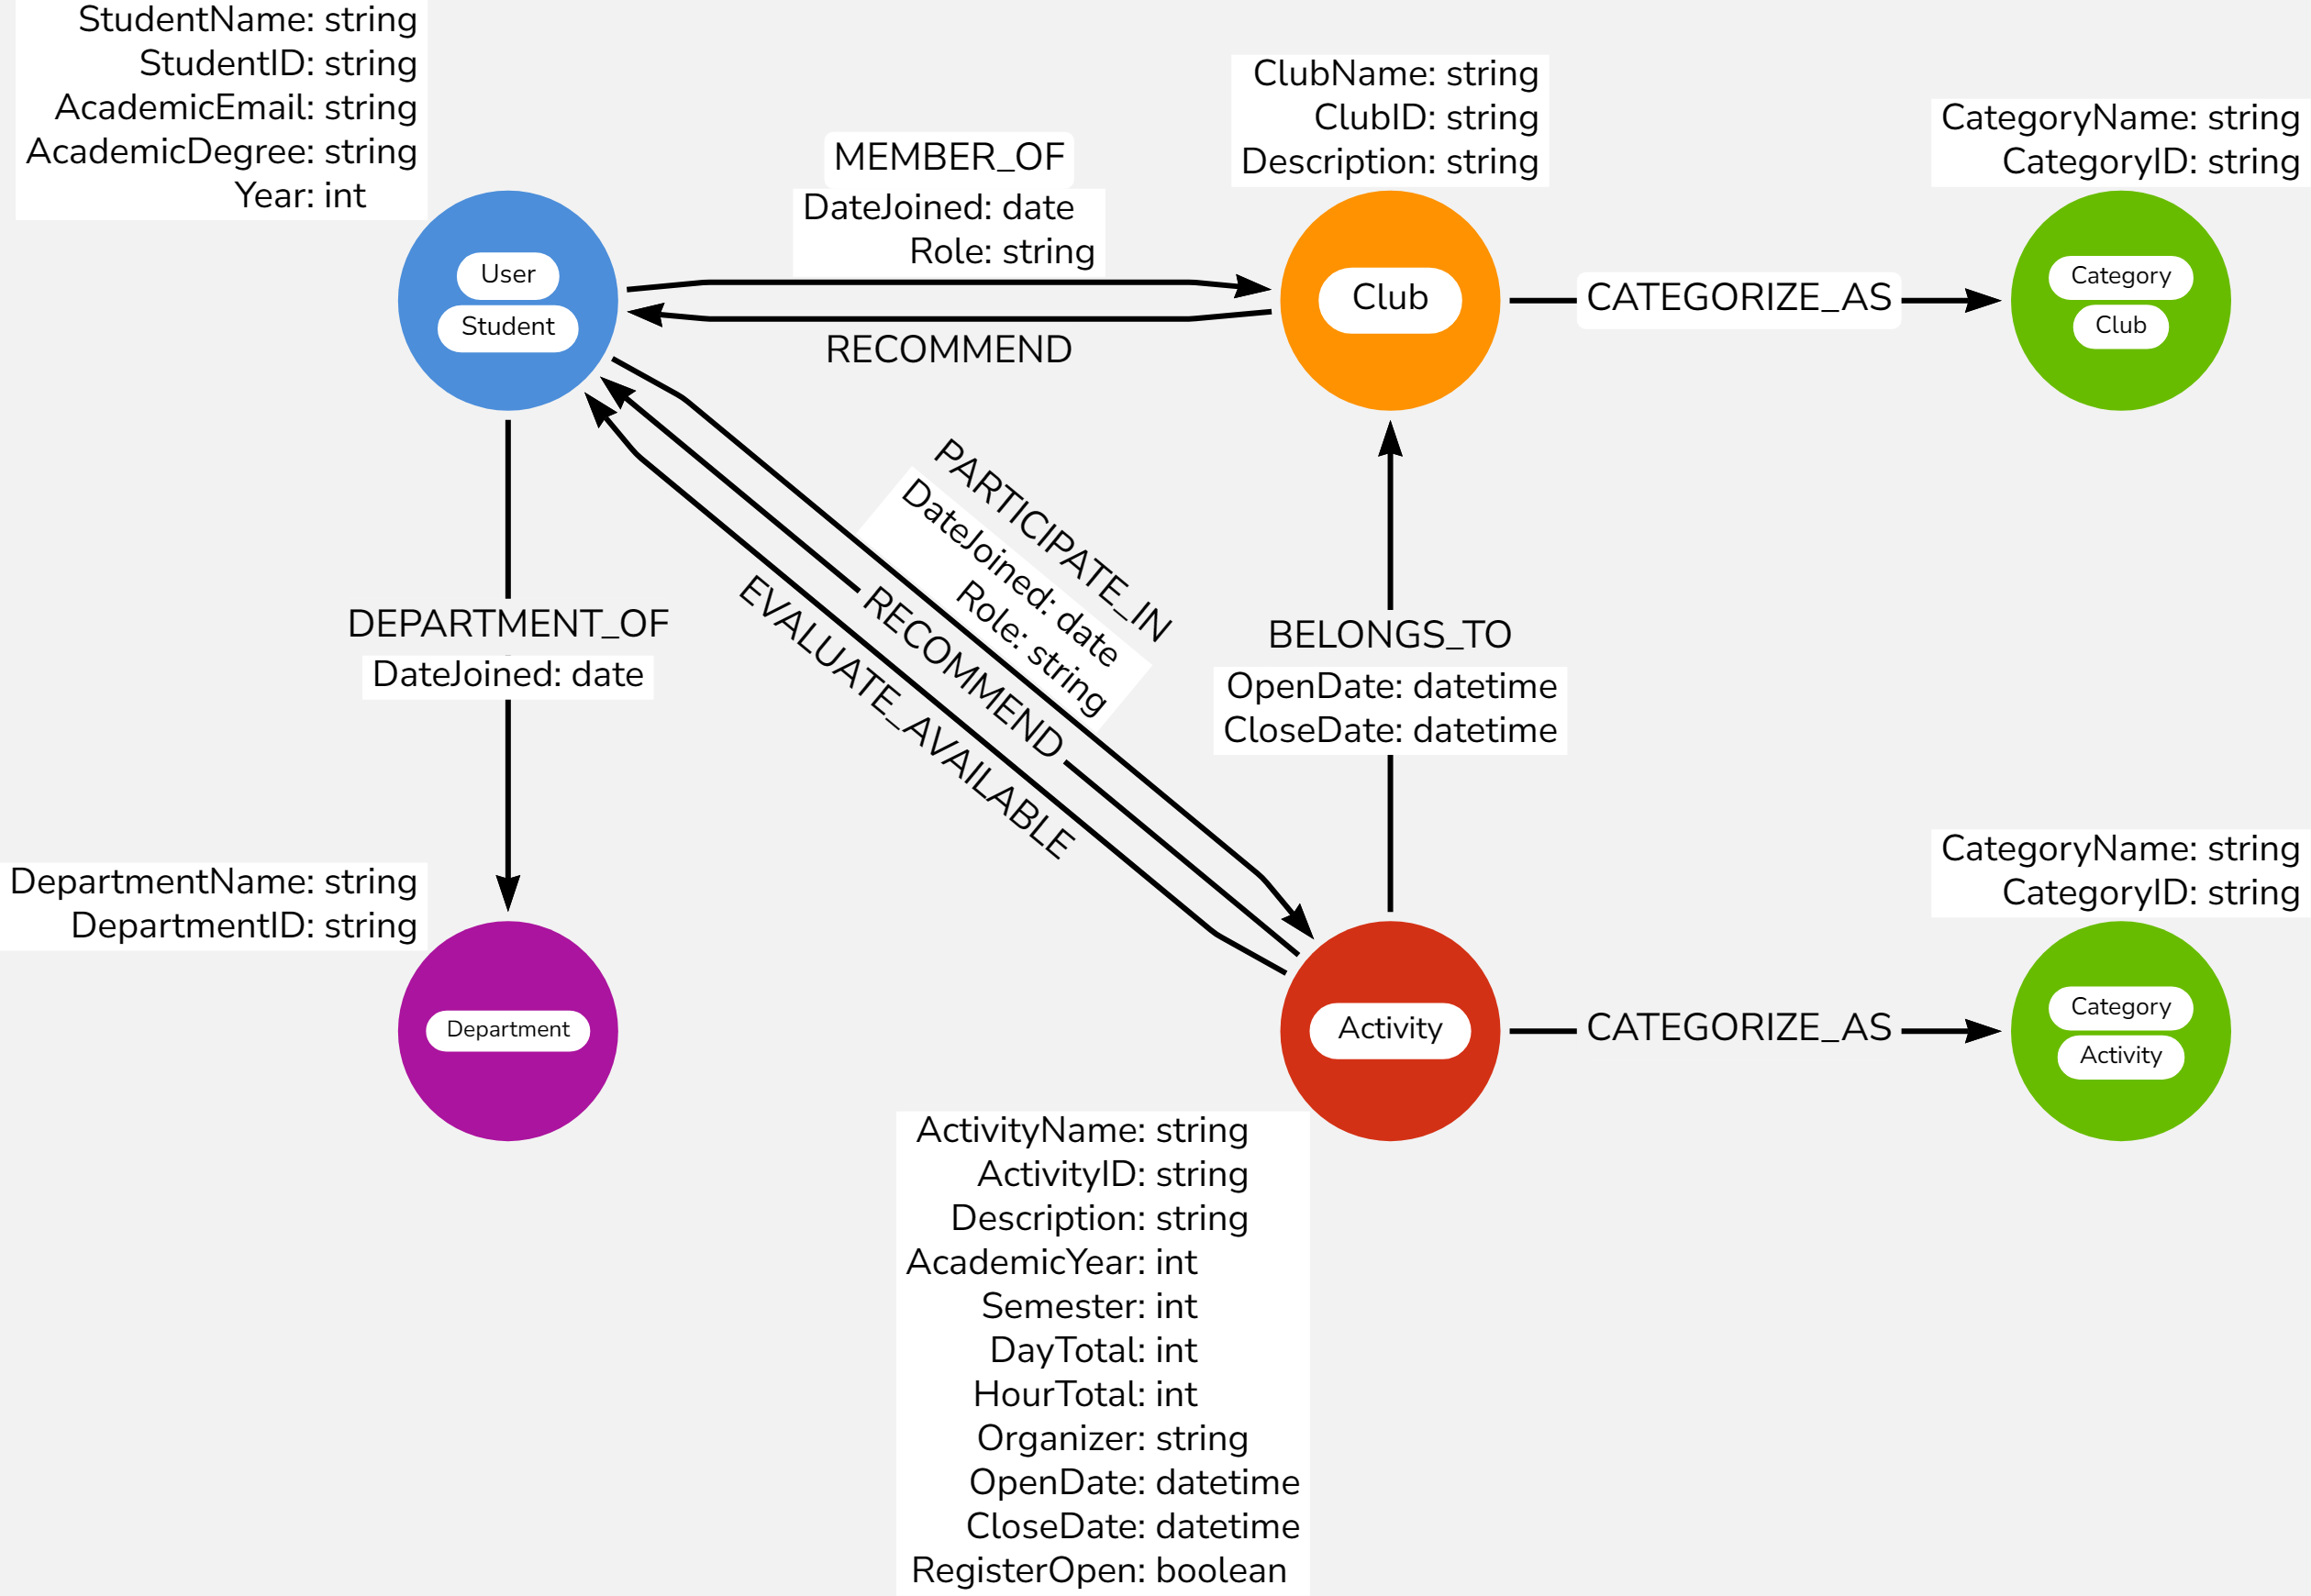
\includegraphics[width=15cm]{./Pictures/DB.png}}
    \caption{Graph Data Model}\label{fig:Graph Data Model}
  \end{figure}
  \FloatBarrier
จากภาพที่ \ref{fig:Graph Data Model} จะเป็นแบบจำลองข้อมูลแบบกราฟของระบบ Actiwiz ซึ่งประกอบไปด้วยโหนด (Node) และความสัมพันธ์ (Relationship) ต่าง ๆ ดังนี้
\newpage
\subsection{โหนด}
    จากที่กล่าวมาโหนดจะทำหน้าที่ในการเก็บข้อมูลซึ่งจะแบ่งข้อมูลในแต่ละโหนดออกมาให้เป็นตารางได้ตามนี้
    \subsubsection{โหนด User: เป็นโหนดที่จะเก็บข้อมูลเกี่ยวกับรายละเอียดส่วนตัวของผู้ใช้งานภายในมหาวิทยาลัย}
    \begin{table}[!h]\centering
      \begin{tabular}{|c|c|c|c|}
      \hline
      \rowcolor[HTML]{9FC5E8} 
      Property       & {\color[HTML]{242424} DataType} & Constain & Definition            \\ \hline
      \cellcolor[HTML]{FFFFFF}{\color[HTML]{242424} StudentName} & \cellcolor[HTML]{FFFFFF}{\color[HTML]{242424} STRING} & Not NULL & ชื่อเต็มของผู้ใช้ \\ \hline
      StudentID      & STRING                          & Not NULL & รหัสนักศึกษาของผู้ใช้ \\ \hline
      AcademicEmail  & STRING                          & Not NULL & อีเมลมหาวิทยาลัย      \\ \hline
      AcademicDegree & STRING                          & Not NULL & ระดับการศึกษา         \\ \hline
      Year           & INTEGER                         & Not NULL & ชั้นปีของนักศึกษา     \\ \hline
      \end{tabular}
      \caption{\centering ตารางเก็บข้อมูลของผู้ใช้งานที่ใช้งานแอปพลิเคชัน}\label{tab:User Node}
    \end{table}
    จากตารางที่ \ref{tab:User Node} แสดงข้อมูลเฉพาะบุคคลของผู้ใช้งานแต่ละคน โดย StudentName นั้นเป็นการจัดเก็บข้อมูลชื่อของนักศึกษาผู้ใช้งาน โดยเก็บข้อมูลเป็นสตริง และยังมีข้อมูลส่วนบุคคลต่าง ๆ ของนักศึกษา เช่น StudentID ที่จัดเก็บรหัสนักศึกษา AcademicEmail จัดเก็บที่อยู่อีเมลของทางมหาลัยที่นักศึกษาคนนั้นใช้งาน และ AcademicDegree ที่จัดเก็บระดับการศึกษาของผู้ใช้งาน ข้อมูลเหล่านี้จะถูกจัดเก็บไว้เป็นสตริงและข้อมูลสุดท้ายที่ถูกจัดเก็บในโหนดนี้คือ Year ซึ่งจะบันทึกข้อมูลชั้นปีของเจ้าของโหนดไว้เป็นจำนวนเต็ม โดยทุกข้อมูลที่เก็บไว้ในโหนดนี้ไม่สามารถถูกเว้นว่างได้
    \subsubsection{โหนด Department: เป็นโหนดที่จะเก็บข้อมูลเกี่ยวกับรายละเอียดของภาควิชาภายในมหาวิทยาลัย}
    \begin{table}[!h]\centering
      \begin{tabular}{|c|c|c|c|}
      \hline
      \rowcolor[HTML]{9FC5E8} 
      Property       & DataType & Constain & Definition                  \\ \hline
      DepartmentName & STRING   & Not NULL & ชื่อภาควิชา                 \\ \hline
      DepartmentID   & STRING   & Not NULL & ชื่อย่อภาษาอังกฤษของภาควิชา \\ \hline
      Description    & STRING   & NULL     & คำอธิบายชมรม                \\ \hline
      \end{tabular}
      \caption{\centering ตารางเก็บข้อมูลของภาควิชาภายในมหาวิทยาลัย}\label{tab:Department Node}
    \end{table}
    จากตารางที่ \ref{tab:Department Node} แสดงข้อมูลเกี่ยวกับรายละเอียดของภาควิชาภายในมหาวิทยาลัยที่ความเชื่อมโยงกับนักศึกษาและกิจกรรมที่จัดขึ้นภายในมหาลัย มีข้อมูลถูกเก็บอยู่ในโหนดนี้ คือ DepartmentName ซึ่งเก็บชื่อของภาควิชา DepartmentID คือชื่อย่อในภาษาอังกฤษของภาควิชานั้น ๆ โดยสองข้อมูลนี้จะถูกจัดเก็บไว้เป็นสตริงโดยจะไม่สามารถถูกเว้นว่างเอาไว้ได้ และข้อมูลสุดท้ายที่ถูกจัดเก็บไว้ในโหนดนี้คือ Description ซึ่งจะเก็บคำอธิบายภาควิชาเอาไว้เป็นสตริง อย่างไรก็ตามข้อมูลนี้สามารถเว้นว่างเอาไว้ได้
    \subsubsection{โหนด Club: เป็นโหนดที่จะเก็บข้อมูลเกี่ยวกับรายละเอียดของชมรมภายในมหาวิทยาลัย}
    \begin{table}[!h]\centering
      \begin{tabular}{|c|c|c|c|}
      \hline
      \rowcolor[HTML]{9FC5E8} 
      Property    & DataType & Constain & Definition   \\ \hline
      ClubName    & STRING   & Not NULL & ชื่อชมรม     \\ \hline
      ClubID      & STRING   & Not NULL & รหัสชมรม     \\ \hline
      Description & STRING   & NULL     & คำอธิบายชมรม \\ \hline
      \end{tabular}
      \caption{\centering ตารางเก็บข้อมูลของชมรมภายในมหาวิทยาลัย}\label{tab:Club Node}
    \end{table}
    จากตารางที่ \ref{tab:Club Node} แสดงข้อมูลเกี่ยวกับรายละเอียดของชมรมภายในมหาวิทยาลัยซึ่งจะเชื่อมโยงไปยังกิจกรรมต่าง ๆ ที่ชมรมเหล่านี้จัดและประเภทของชมรมที่ทางผู้จัดทำได้แบ่งประเภทเอาไว้ ข้อมูลที่เก็บไว้ในโหนดเหล่านี้ ได้แก่ ClubName บันทึกข้อมูลของชื่อชมรมที่มีเอาไว้ ClubID จะเก็บข้อมูลรหัสของชมรมเอาไหว้ โดยข้อมูลทั้งสองส่วนนี้จัดเก็บไว้เป็นสตริงแต่ไม่สามารถเว้นข้อมูลให้ว่างไว้ได้ และข้อมูลสุดท้ายที่ถูกจัดเก็บไว้ในโหนดนี้คือ Description หรือคำอธิบายชมรมที่จะบันทึกเป็นสตริง แต่สามารถเว้นข้อมูลส่วนนี้เอาไว้ได้
    \subsubsection{โหนด Club Category: เป็นโหนดที่จะเก็บข้อมูลเกี่ยวกับรายละเอียดประเภทชมรมภายในมหาวิทยาลัย}
    \begin{table}[!h]\centering
      \begin{tabular}{|c|c|c|c|}
      \hline
      \rowcolor[HTML]{9FC5E8} 
      Property       & {\color[HTML]{242424} DataType} & Constain & Definition        \\ \hline
      \cellcolor[HTML]{FFFFFF}{\color[HTML]{242424} CategoryName} & \cellcolor[HTML]{FFFFFF}{\color[HTML]{242424} STRING} & Not NULL & ชื่อประเภท \\ \hline
      CategoryID     & STRING                          & Not NULL & รหัสประเภท        \\ \hline
      Description    & STRING                          & NULL     & คำอธิบายประเภทชมรม      \\ \hline
      \end{tabular}
      \caption{\centering ตารางเก็บข้อมูลประเภทชมรม}\label{tab:Club Category Node}
    \end{table}
    จากตารางที่ \ref{tab:Club Category Node} แสดงข้อมูลเกี่ยวกับรายละเอียดประเภทชมรมภายในมหาวิทยาลัยซึ่งทางผู้จัดทำพยายามจัดแบ่งโดยอาศัยจากทั้งชื่อโครงการและคำอธิบายโครงการใช้เพื่อสื่อสารกับผู้ที่เข้าร่วมกิจกรรมที่ชมรมจัดหรือสมาชิคชมรม โดยจะมีข้อมูลที่ถูกจัดเก็บไว้ ได้แก่ CategoryID หรือรหัสของประเภทชมรมที่จะถูกจัดเก็บไว้เป็นสตริง และอีกส่วนคือ Description คำอธิบายของประเภทชมรมจะถูกบันทึกเป็นสตริงแต่อนุญาติให้เว้นว่างข้อมูลในส่วนนี้เอาไว้ได้
    \subsubsection{โหนด Activity: เป็นโหนดที่จะเก็บข้อมูลเกี่ยวกับรายละเอียดของกิจกรรมภายในมหาวิทยาลัย}
    \begin{table}[!h]\centering
      \begin{tabular}{|c|c|c|c|}
      \hline
      \rowcolor[HTML]{9FC5E8} 
      Property     & DataType & Constain & Definition                              \\ \hline
      ActivityName & STRING   & Not NULL & ชื่อกิจกรรม                            \\ \hline
      ActivityID   & STRING   & Not NULL & รหัสกิจกรรม                              \\ \hline
      Description  & STRING   & NULL     & คำอธิบายกิจกรรม                         \\ \hline
      AcademicYear & INTEGER  & Not NULL & ปีการศึกษา                              \\ \hline
      Semester     & INTEGER  & Not NULL & ภาคการศึกษา                             \\ \hline
      DayTotal     & INTEGER  & Not NULL & จำนวนวันของกิจกรรม                      \\ \hline
      HourTotal    & INTEGER  & Not NULL & จำนวนชั่วโมงกิจกรรม                     \\ \hline
      Organizer    & STRING   & Not NULL & ชื่อผู้จัดกิจกรรม                       \\ \hline
      OpenDate     & DATETIME & Not NULL & วันแรกของกิจกรรม                        \\ \hline
      CloseDate    & DATETIME & Not NULL & วันสุดท้ายของกิจกรรม                    \\ \hline
      RegisterOpen & BOOLEAN  & Not NULL & สถานะของการเปิดลงทะเบียนเข้าร่วมกิจกรรม \\ \hline
      \end{tabular}
      \caption{\centering ตารางเก็บข้อมูลของชมรมภายในมหาวิทยาลัย}\label{tab:Activitynode}
    \end{table}
    จากตารางที่ \ref{tab:Activitynode} แสดงข้อมูลที่ถูกจัดเก็บไว้ในโหนดนี้คือข้อมูลเกี่ยวกับรายละเอียดของกิจกรรมต่าง ๆ ที่ถูกจัดขึ้นภายในมหาวิทยาลัย มีข้อมูลรายละเอียดต่าง ๆ แจกแจงออกมาเป็น ActivityName จะจัดเก็บชื่อกิจกรรมเอาไว้เป็นสตริง โดยไม่สามารถละข้อมูลเอาไว้ได้ ActivityID เก็บ ID ของกิจกรรมเอาไว้เป็นสตริงซึ่งไม่สามารถล่ะข้อมูลเอาไว้ได้เช่นกัน Description จะจัดเก็บคำอธิบายของโครง
    การซึ่งเป็นข้อมูลเดียวในโหนดนี้ที่สามารถเว้นว่างไว้ได้ AcademicYear จะบันทึกปีการศึกษาที่กิจกรรมที่จัดกิจกรรมนั้น ๆ ขึ้นมาเป็นจำนวนเต็ม Semester จะบันทึกภาคการศึกษาที่จัดกิจกรรมนั้น ๆ ขึ้นเป็นจำนวนเต็ม DayTotal จะบันทึกจำนวนวันที่ใช้จัดกิจกรรมจะถูกบันทึกเป็นจำนวนเต็ม HourTotal จะบันทึกจำนวนชั่วโมงที่ใช้จัดกิจกรรมจะถูกบันทึกเป็นจำนวนเต็ม Organizer จะบันทึกชื่อขององค์กรผู้ที่จัดกิจกรรมไว้เป็นสตริง OpenDate จะบันทึกผู้มูลเวลาของวันที่เริ่มกิจกรรมเอาไว้ CloseDate จะบันทึกผู้มูลเวลาของวันที่กิจกรรมจบลงเอาไว้ RegisterOpen จะบันทึกวันที่เปิดให้ลงทะเบียนเข้าร่วมกิจกรรมเอาไว้
    \newpage
    \subsubsection{โหนด Activity Category: เป็นโหนดที่จะเก็บข้อมูลเกี่ยวกับประเภทของกิจกรรมภายในมหาวิทยาลัย}
    \begin{table}[!h]\centering
      \begin{tabular}{|c|c|c|c|}
      \hline
      \rowcolor[HTML]{9FC5E8} 
      Property     & DataType & Constain & Definition \\ \hline
      CategoryName & STRING   & Not NULL & ชื่อประเภท \\ \hline
      CategoryID   & STRING   & Not NULL & รหัสประเภท \\ \hline
      \end{tabular}
      \caption{\centering ตารางเก็บข้อมูลประเภทของกิจกรรม}\label{tab:Activity Category Node}
    \end{table}
    จากตารางที่ \ref{tab:Activity Category Node} แสดงข้อมูลที่ถูกจัดเก็บไว้ในโหนดนี้คือข้อมูลเกี่ยวกับรายละเอียดประเภทกิจกรรมต่าง ๆ ที่ถูกจัดขึ้นภายในมหาวิทยาลัยซึ่งทางผู้จัดทำพยายามจัดแบ่งโดยอาศัยจากทั้งชื่อโครงการและคำอธิบายโครงการใช้เพื่อสื่อสารกับผู้ที่เข้าร่วมกิจกรรม โดยจะมีข้อมูลที่ถูกจัดเก็บไว้ ได้แก่ CategoryID หรือรหัสของประเภทกิจกรรมที่จะถูกจัดเก็บไว้เป็นสตริง และอีกส่วนคือ Description คำอธิบายของประเภทกิจกรรมจะถูกบันทึกเป็นสตริงแต่อนุญาติให้เว้นว่างข้อมูลในส่วนนี้เอาไว้ได้
    \subsection{ความสัมพันธ์}
    ความสัมพันธ์ภายในแบบจำลองข้อมูลแบบกราฟของแอพพลิเคชัน Actiwiz เป็นการสร้างความเชื่อมโยงและการมีปฏิสัมพันธ์ระหว่างโหนดต่าง ๆ ซึ่งมีส่วนช่วยในการนำเสนอเรื่องราวการเข้าร่วมกิจกรรมและชมรมภายในมหาวิทยาลัยแบบยืดหยุ่นและเชื่อมโยงถึงกัน โดยความสัมพันธ์จะมีอยู่ 2 รูปแบบด้วยกัน ได้แก่ความสัมพันธ์ที่มีคุณสมบัติที่บอกข้อมูลเพิ่มเติมและความสัมพันธ์ที่ไม่มีคุณสมบัติเพิ่มเติม

    \subsubsection{ความสัมพันธ์ที่มีคุณสมบัติ}
    \begin{itemize}
      \normalsize
      \item User is in DEPARTMENT\_OF Department: ความสัมพันธ์ DEPARTMENT\_OF แสดงความสัมพันธ์ทางวิชาการของผู้ใช้งานกับภาควิชาของตน ความสัมพันธ์นี้ช่วยเชื่อมโยงผู้คนจากภาควิชาเดียวกันภายในมหาวิทยาลัย
        \begin{center}
          \begin{tabular}{|c|c|c|c|}
          \hline
          \rowcolor[HTML]{9FC5E8} 
          Property   & DataType & Constraint & Definition \\ \hline
          DateJoined & DATE     & Not NULL    & วันที่เข้าเป็นนักศึกษาของภาควิชา \\ \hline
          \end{tabular}
          \captionof{table}{ตารางเก็บข้อมูลนักศึกษาภาควิชา}\label{tab:DepartmentRelationship}
        \end{center}
        จากตารางที่ \ref{tab:DepartmentRelationship} แสดงข้อมูลที่ถูกจัดเก็บไว้แสดงความสัมพันธ์ทางวิชาการของผู้ใช้งานกับภาควิชาของตน ความสัมพันธ์นี้ช่วยเชื่อมโยงผู้คนจากภาควิชาเดียวกันภายในมหาวิทยาลัย โดยมีคุณสมบัตติที่บันทึกไว้ในความสัมพันธ์นี้คือ DateJoined ที่บันทึกข้อมูลวันเวลาที่ผู้ใช้งานเข้าร่วมภาควิชานั้น ๆ ซึ่งข้อมูลในส่วนนี้ไม่สามารถเว้นเอาไว้ได้ 
      \item User is a MEMBER\_OF Club: ความสัมพันธ์ MEMBER\_OF แสดงความสัมพันธ์ของผู้ใช้งานว่าเป็นหนึ่งในสมาชิกของชมรมใดชมรมหนึ่ง
        \begin{center}
          \begin{tabular}{|c|c|c|c|}
          \hline
          \rowcolor[HTML]{9FC5E8} 
          Property   & DataType & Constraint & Definition \\ \hline
          DateJoined & DATE     & Not NULL    & วันที่เริ่มเป็นสมาชิกชมรม \\ \hline
          Role       & STRING   & Not NULL    & ตำแหน่งในชมรม \\ \hline
          \end{tabular}
          \captionof{table}{ตารางเก็บข้อมูลสมาชิกของชมรม}\label{tab:ClubRelationship}
        \end{center}
        จากตารางที่ \ref{tab:ClubRelationship} แสดงข้อมูลที่ถูกจัดเก็บไว้แสดงความสัมพันธ์ของผู้ใช้งานว่าเป็นหนึ่งในสมาชิกของชมรมใดชมรมหนึ่ง ความสัมพันธ์นี้ช่วยเชื่อมโยงผู้คนที่ชมรมเดียวกัน โดยมีคุณสมบัตติที่บันทึกไว้ในความสัมพันธ์นี้คือ DATE ที่บันทึกข้อมูลวันเวลาที่ผู้ใช้งานเข้าร่วมชมรมนั้น ๆ และ Role จะบันทึกตำแหน่งของผู้ใช้งานในชมรมนั้นเอาไว้เป็นสตริง โดยทั้งสองข้อมูลนี้ไม่สามารถเว้นว่างเอาไว้ได้ทั้งคู่
      \newpage
        \item User PARTICIPATE\_IN Activity: ความสัมพันธ์ PARTICIPATES\_IN แสดงถึงการเข้าร่วมกิจกรรมของผู้ใช้งานในกิจกรรมต่าง ๆ ภายในมหาวิทยาลัย
        \begin{center}
          \begin{tabular}{|c|c|c|c|}
          \hline
          \rowcolor[HTML]{9FC5E8} 
          DateJoined & DataType & Constraint & Definition \\ \hline
          DateJoined & DATE     & Not NULL    & วันที่เข้าร่วมกิจกรรม \\ \hline
          Role       & STRING   & Not NULL    & ตำแหน่งในกิจกรรม \\ \hline
          \end{tabular}
          \captionof{table}{ตารางเก็บข้อมูลสมาชิกเข้าร่วมกิจกรรม}\label{tab:ActivityRelationship}
        \end{center}
        จากตารางที่ \ref{tab:ActivityRelationship} แสดงข้อมูลที่ถูกจัดเก็บไว้แสดงความสัมพันธ์ของผู้ใช้งานว่าเข้าร่วมกิจกรรมใดบ้าง ความสัมพันธ์นี้ช่วยเชื่อมโยงผู้คนที่่เคยเข้าร่วมกิจกรรมเดียวกัน โดยมีคุณสมบัตติที่บันทึกไว้ในความสัมพันธ์นี้คือ DATE ที่บันทึกข้อมูลวันเวลาที่ผู้ใช้งานเข้าร่วมกิจกรรมนั้น ๆ และ Role จะบันทึกบทบาทของผู้ใช้งานในกิจกรรมนั้น ๆ เอาไว้เป็นสตริง โดยทั้งสองข้อมูลนี้ไม่สามารถเว้นว่างเอาไว้ได้ทั้งคู่
        \item Activity BELONGS\_TO Club: ความสัมพันธ์ BELONGS\_TO แสดงความสัมพันธ์ระหว่างกิจกรรมกับชมรม โดยระบุว่าชมรมใดรับผิดชอบในการจัดกิจกรรมใดกิจกรรมหนึ่ง
        \begin{center}
          \begin{tabular}{|c|c|c|c|}
          \hline
          \rowcolor[HTML]{9FC5E8} 
          Property   & DataType & Constraint & Definition \\ \hline
          OpenDate   & DATETIME & Not NULL    & วันแรกของกิจกรรม \\ \hline
          CloseDate  & DATETIME & Not NULL    & วันสุดท้ายของกิจกรรม \\ \hline
          \end{tabular}
          \captionof{table}{ตารางเก็บข้อมูลกิจกรรมถูกจัดโดยชมรม}\label{tab:ClubActivityRelationship}
        \end{center}
        จากตารางที่ \ref{tab:ClubActivityRelationship} แสดงข้อมูลที่ถูกจัดเก็บไว้แสดงความสัมพันธ์ระหว่างผู้จัดกิจกรรมกับกิจกรรมต่าง ๆ ที่ถูกจัดขึ้น ความสัมพันธ์นี้บอกถึงความเกี่ยวข้องกันของกิจกรรมและชมรมต่าง ๆ ในมหาวิทยาลัย โดยมีคุณสมบัตติที่บันทึกไว้ในความสัมพันธ์นี้คือ OpenDate ที่บันทึกข้อมูลวันเวลาที่เริ่มต้นกิจกรรมนั้น และ CloseDate จะบันทึกวันเวลาที่กิจกรรมนั้นสิ้นสุดลง โดยทั้งสองข้อมูลนี้ไม่สามารถเว้นว่างเอาไว้ได้ทั้งคู่
    \end{itemize}    
      \subsubsection{ความสัมพันธ์ที่ไม่มีคุณสมบัติ}
        \normalsize
        \begin{itemize}
          \item Activity CATEGORIZE\_AS Activity Category: ความสัมพันธ์ CATEGORIZE\_AS จัดกลุ่มกิจกรรมด้วยการจัดประเภทของกิจกรรม ตามหมวดหมู่เนื้อหา
          \item Activity RECOMMEND to User: ความสัมพันธ์ RECOMMEND แสดงถึงการแนะนำกิจกรรมที่สร้างโดยระบบของแอปพลิเคชัน โดยเกิดจากการประมวลผลของ machine learning ที่ปรับให้เหมาะสมตามผู้ใช้งานแต่ละคน
          \item Activity EVALUATE\_AVAILABLE to User: ความสัมพันธ์แบบ EVALUATE\_AVAILABLE จะเชื่อมโยงผู้ใช้เข้ากับกิจกรรมต่าง ๆ เมื่อกิจกรรมเปิดให้ผู้ใช้งานเข้าไปประเมินกิจกรรมได้
          \item Club CATEGORIZE\_AS Club Category: ความสัมพันธ์ CATEGORIZE\_AS จัดกลุ่มชมรมด้วยการจัดประเภทของชมรม ตามหมวดหมู่เนื้อหา
          \item Club RECOMMEND to User: ความสัมพันธ์ RECOMMEND แสดงถึงการแนะนำชมรมที่สร้างโดยระบบของแอปพลิเคชัน โดยเกิดจากการประมวลผลของ machine learning ที่ปรับให้เหมาะสมตามผู้ใช้งานแต่ละคน
        \end{itemize}
\chapter{ผลการทดลองและอภิปรายผล} 
ในบทนี้จะกล่าวถึงผลลัพธ์จากการทดสอบฟังก์ชันหลักของระบบในแอปพลิเคชัน รวมถึงความสามารถในการทำงาน ความเหมาะสมในการใช้งาน การตอบสนองต่อผู้ใช้ และความพึงพอใจของผู้ใช้
\section{การเปลี่ยนแปลงรายละเอียดของโครงการ}
รายละเอียดของโครงการที่เปลี่ยนแปลงไปจากภาคการศึกษาที่ 1 ประกอบไปด้วยส่วนของการออกแบบแอปพลิเคชันต่าง ๆ ดังนี้
 \subsection{รายการคุณลักษณะ (Feature List)}\label{subsec:editedfeaturelist}
 ด้วยวัตถุประสงค์เพื่อเพิ่มประสิทธิภาพและความสะดวกสบายแก่ผู้ใช้งานแอปพลิเคชัน ทางผู้จัดทำจึงได้มีการตัดสินใจให้มีการยกเลิกรูปแบบการให้ผู้ใช้งานลงทะเบียนสมาชิกใหม่สำหรับแอปพลิเคชัน และดำเนินการปรับเปลี่ยนกระบวนการการเข้าสู่ระบบ (Login) และการพิสูจน์ยืนยันตัวตน (Authenticate) ของผู้ใช้งาน
 ให้เป็นการดำเนินการผ่านระบบ Microsoft Entra ID ซึ่งเป็นระบบจัดการการพิสูจน์ยืนยันตัวตนแบบรวมศูนย์ที่ทันสมัยและได้รับการยอมรับในระดับสากล โดยผู้ใช้งานจะสามารถใช้บัญชี Kmutt Internet Account ซึ่งเป็นบัญชีที่ผู้ใช้งานได้ลงทะเบียนไว้กับมหาวิทยาลัยเป็นที่เรียบร้อยแล้ว 
 ในการเข้าสู่ระบบและพิสูจน์ยืนยันตัวตน โดยไม่จำเป็นต้องลงทะเบียนบัญชีสมาชิกใหม่กับแอปพลิเคชันอีกเป็นครั้งที่สอง ด้วยการปรับเปลี่ยนรูปแบบการให้บริการในครั้งนี้จะส่งผลให้ผู้ใช้งานได้รับความสะดวกสบายมากยิ่งขึ้น อีกทั้งยังเป็นการเพิ่มระดับความปลอดภัยในการเข้าถึงข้อมูลส่วนบุคคลของผู้ใช้งานผ่านกระบวนการพิสูจน์ยืนยันตัวตนที่ได้มาตรฐานสากล
 \subsection{เเผนภาพที่ใช้เเสดงปฎิสัมพันธ์ระหว่างระบบงานเเละสิ่งที่อยู่นอกระบบงาน (Use Case Diagram)}
   \begin{figure}[H]\centering
    \setlength{\fboxrule}{0.5mm} % can define this in the preamble
    \setlength{\fboxsep}{0.5cm}
    \fbox{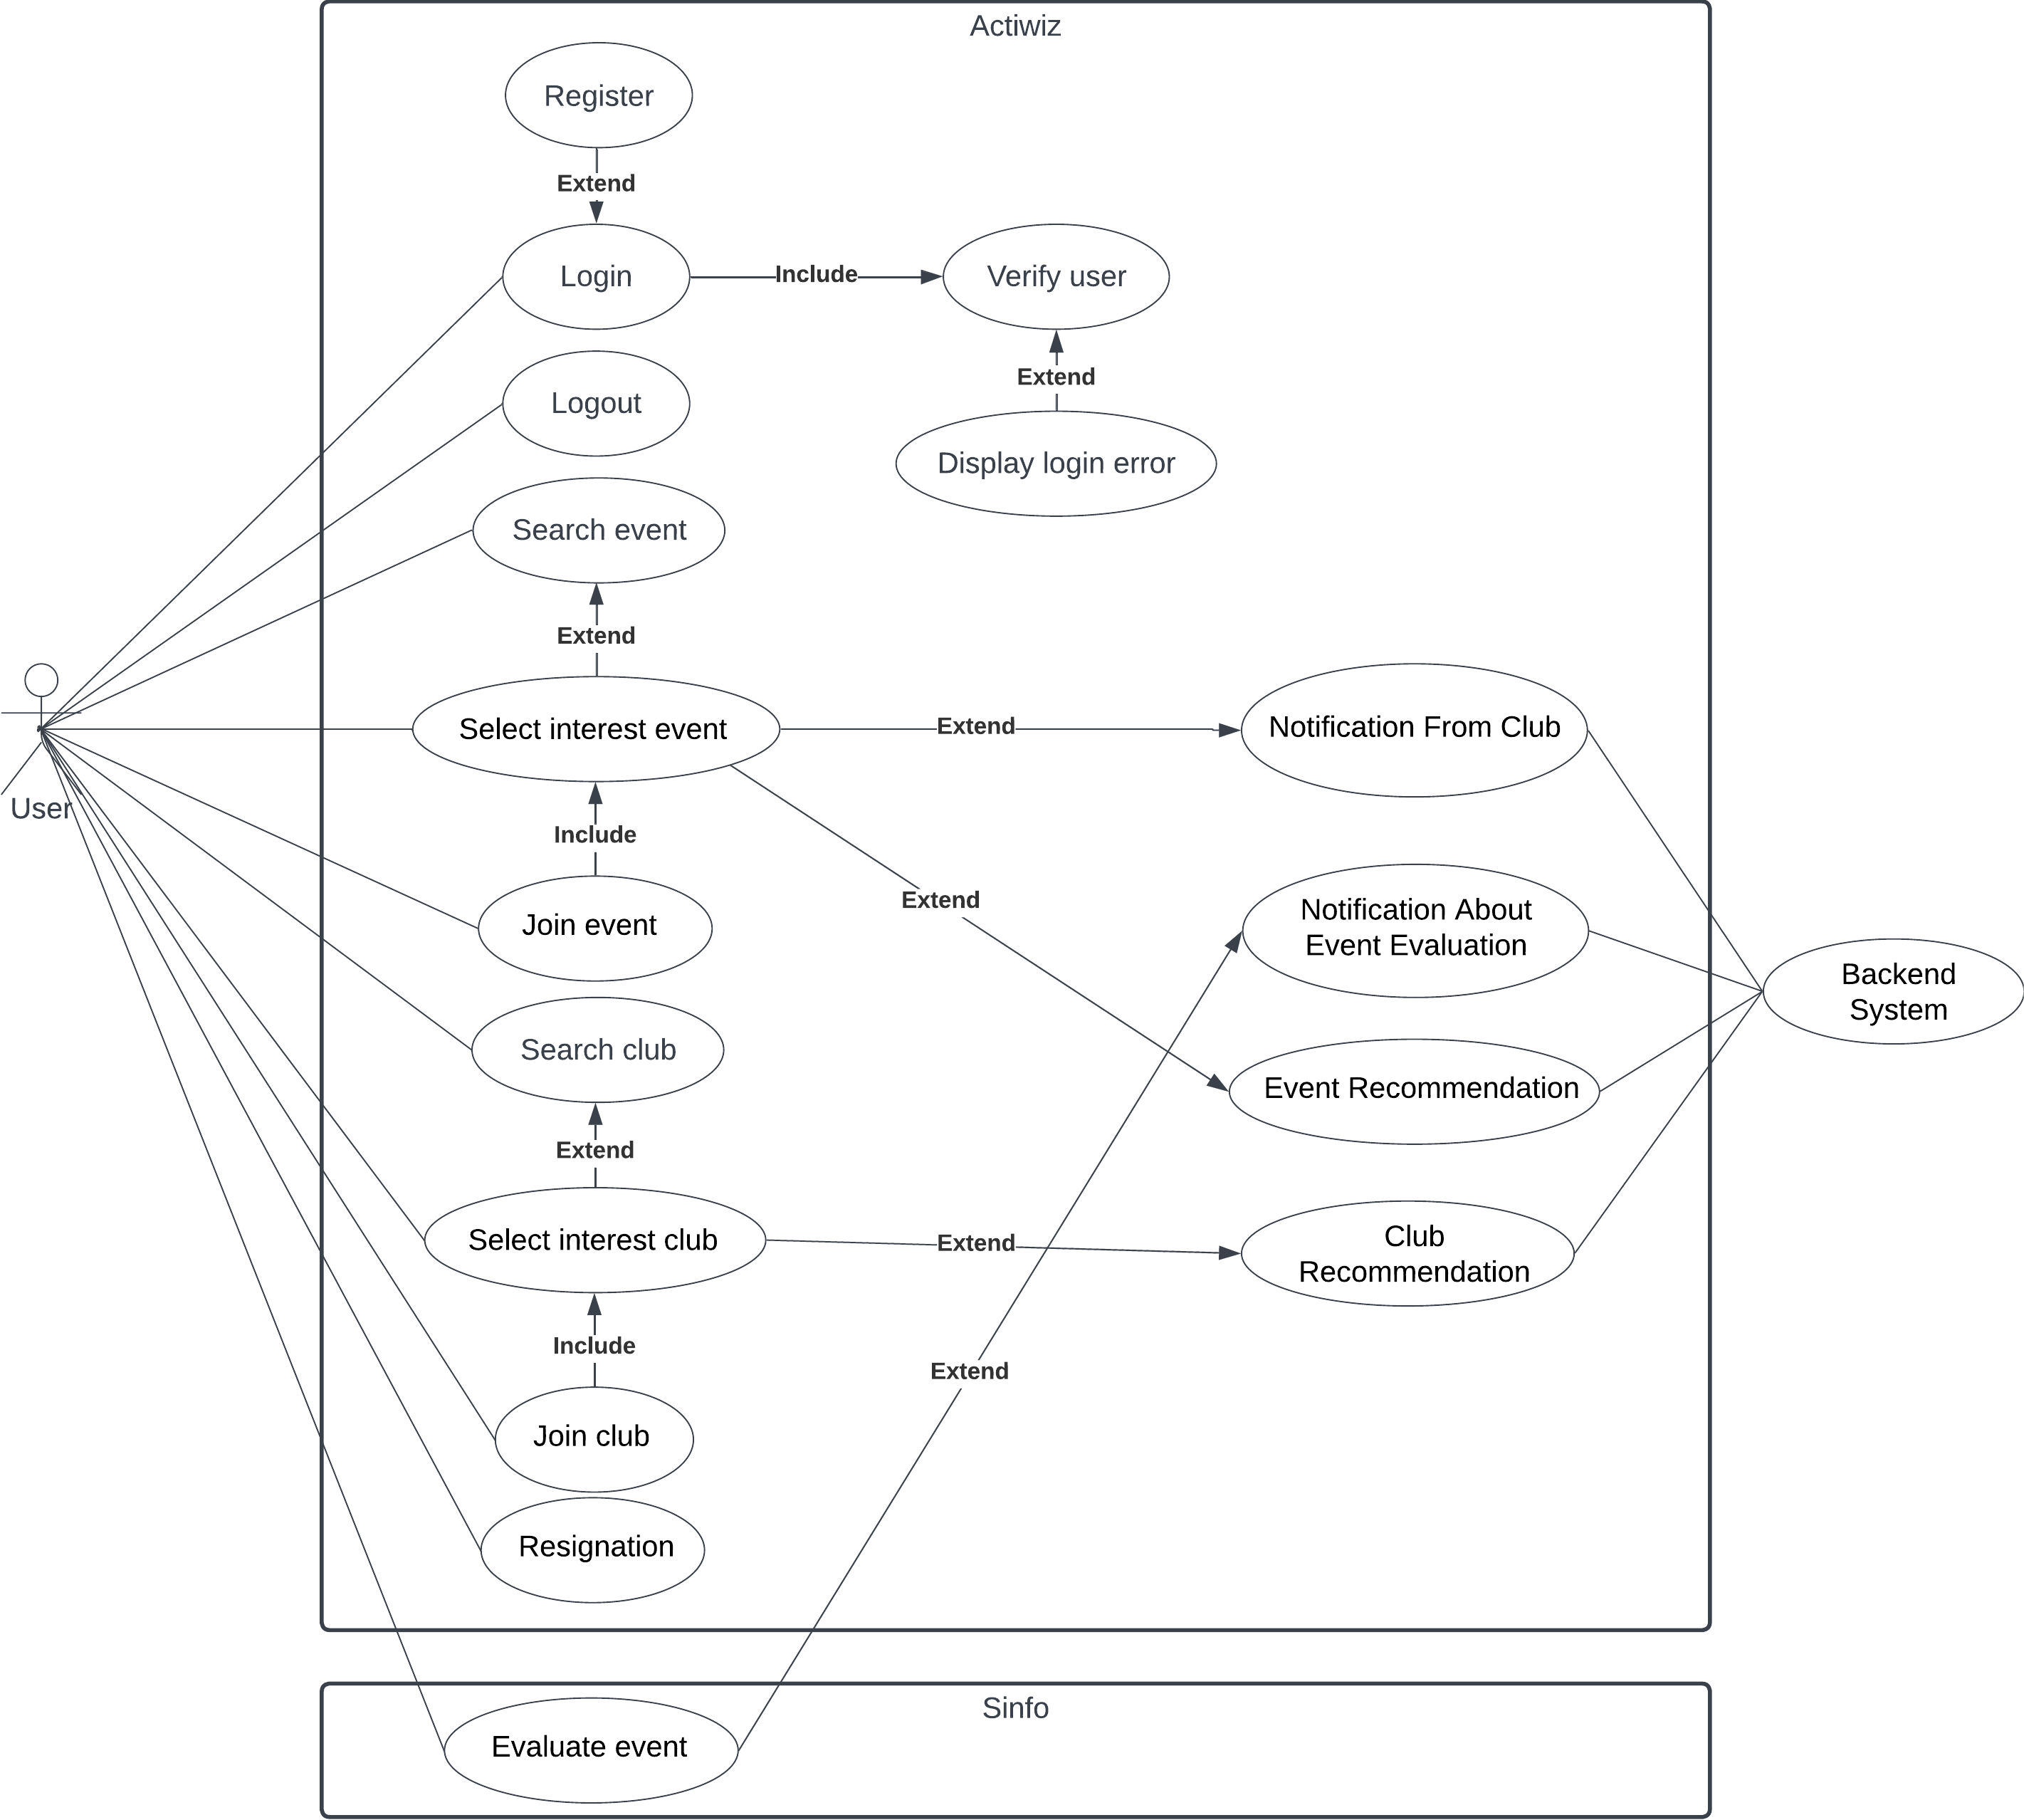
\includegraphics[width=12.5cm]{./Pictures/V4_Use_Cases_Diagram.png}}
    \caption{Edited Use Case Diagram}\label{fig:editedusecasediagram}
   \end{figure}
  ทางผู้จัดทำได้มีการปรับปรุงเเผนภาพที่ใช้เเสดงปฎิสัมพันธ์ระหว่างระบบงานเเละสิ่งที่อยู่นอกระบบงาน (Use Case Diagram) จากภาพที่ \ref{fig:usecasediagram} มาเป็นรูปที่ \ref{fig:editedusecasediagram} แทน 
  เนื่องด้วยเหตุผลสำคัญตามการเปลี่ยนแปลงที่ได้กล่าวไปในหัวข้อที่ \ref{subsec:editedfeaturelist} ด้วยเหตุนี้จึงไม่มีความจำเป็นที่จะต้องให้ผู้ใช้งานลงทะเบียนบัญชีใหม่เพิ่มเติมกับแอปพลิเคชันอีกครั้ง 
  เพื่อเข้าใช้งานระบบของแอปพลิเคชัน อันเป็นผลให้สามารถนำ Use Case ที่เกี่ยวข้องกับการลงทะเบียน หรือ Register Use Case ที่ปรากฏในรูปที่ \ref{fig:usecasediagram} ออกไปได้ เนื่องจากไม่มีความจำเป็นต่อการทำงานของระบบอีกต่อไป
  \\ \\
  \textbf{Use Case Narratives}
  \begin{table}[!h]\centering
    \begin{tabular}{|c|c|}
    \hline
    \rowcolor[HTML]{9FC5E8} 
    Actor                       & {\color[HTML]{242424} User}                                                                                          \\ \hline
    \rowcolor[HTML]{FFFFFF} 
    {\color[HTML]{242424} Goal} & {\color[HTML]{242424} เข้าสู่ระบบและใช้งานฟังก์ชันต่างได้}                                                           \\ \hline
    Pre-conditions              & - \\ \hline
    Main success scenario &
      \begin{tabular}[c]{@{}c@{}}1.User กดปุ่มเพื่อไปยังหน้า Login ของ Microsoft \\ 2.User กรอกอีเมลและรหัสผ่าน\\ 3.User เข้าสู่ homepage ของแอปพลิเคชัน\\ 4.ระบบแสดงฟังก์ชันที่ใช้งานได้ทั้งหมด\\ 5.User ใช้งานฟังก์ชันต่าง ๆ ในแอปพลิเคชัน\end{tabular} \\ \hline
    \end{tabular}
    \caption{\centering การเข้าสู่ระบบ}\label{tab:Edited Login scenario}
  \end{table}
  \\
  สำหรับส่วนการบรรยายรายละเอียดเกี่ยวกับกรณีการใช้งานระบบต่าง ๆ ไม่มีความจำเป็นที่จะต้องอธิบายรายละเอียดของ Use Case ที่เกี่ยวกับการลงทะเบียนแล้ว ส่งผลให้ตารางที่ \ref{tab:Registration scenario} ซึ่งเป็นตารางสำหรับการอธิบายรายละเอียดของการสมัครเข้าใช้งานระบบไม่มีความจำเป็นต่อการใช้งานอีกต่อไป
  นอกจากนี้ การเปลี่ยนแปลงรูปแบบการให้บริการดังกล่าวยังส่งผลให้รายละเอียดของตารางที่ \ref{tab:Login scenario} ซึ่งเป็นตารางสำหรับการอธิบายรายละเอียดของการเข้าสู่ระบบมีการเปลี่ยนแปลงเล็กน้อย โดยจะมีการเพิ่มขั้นตอนของการเข้าสู่ระบบ (Login) ผ่านระบบของ Microsoft เป็นอันดับแรกก่อนการกรอกรายละเอียดของผู้ใช้เพื่อทำการเข้าสู่ระบบ 
  ดังปรากฏในรูปแบบตามตารางที่ \ref{tab:Edited Login scenario} ทั้งนี้เพื่อให้สอดคล้องกับกระบวนการทำงานของระบบที่ได้มีการปรับเปลี่ยนไป
  \subsection{เเผนภาพที่ใช้เเสดงการทำงานของระบบ (Sequence Diagram)}
   \begin{figure}[H]\centering
    \setlength{\fboxrule}{0.5mm} % can define this in the preamble
    \setlength{\fboxsep}{0.5cm}
    \fbox{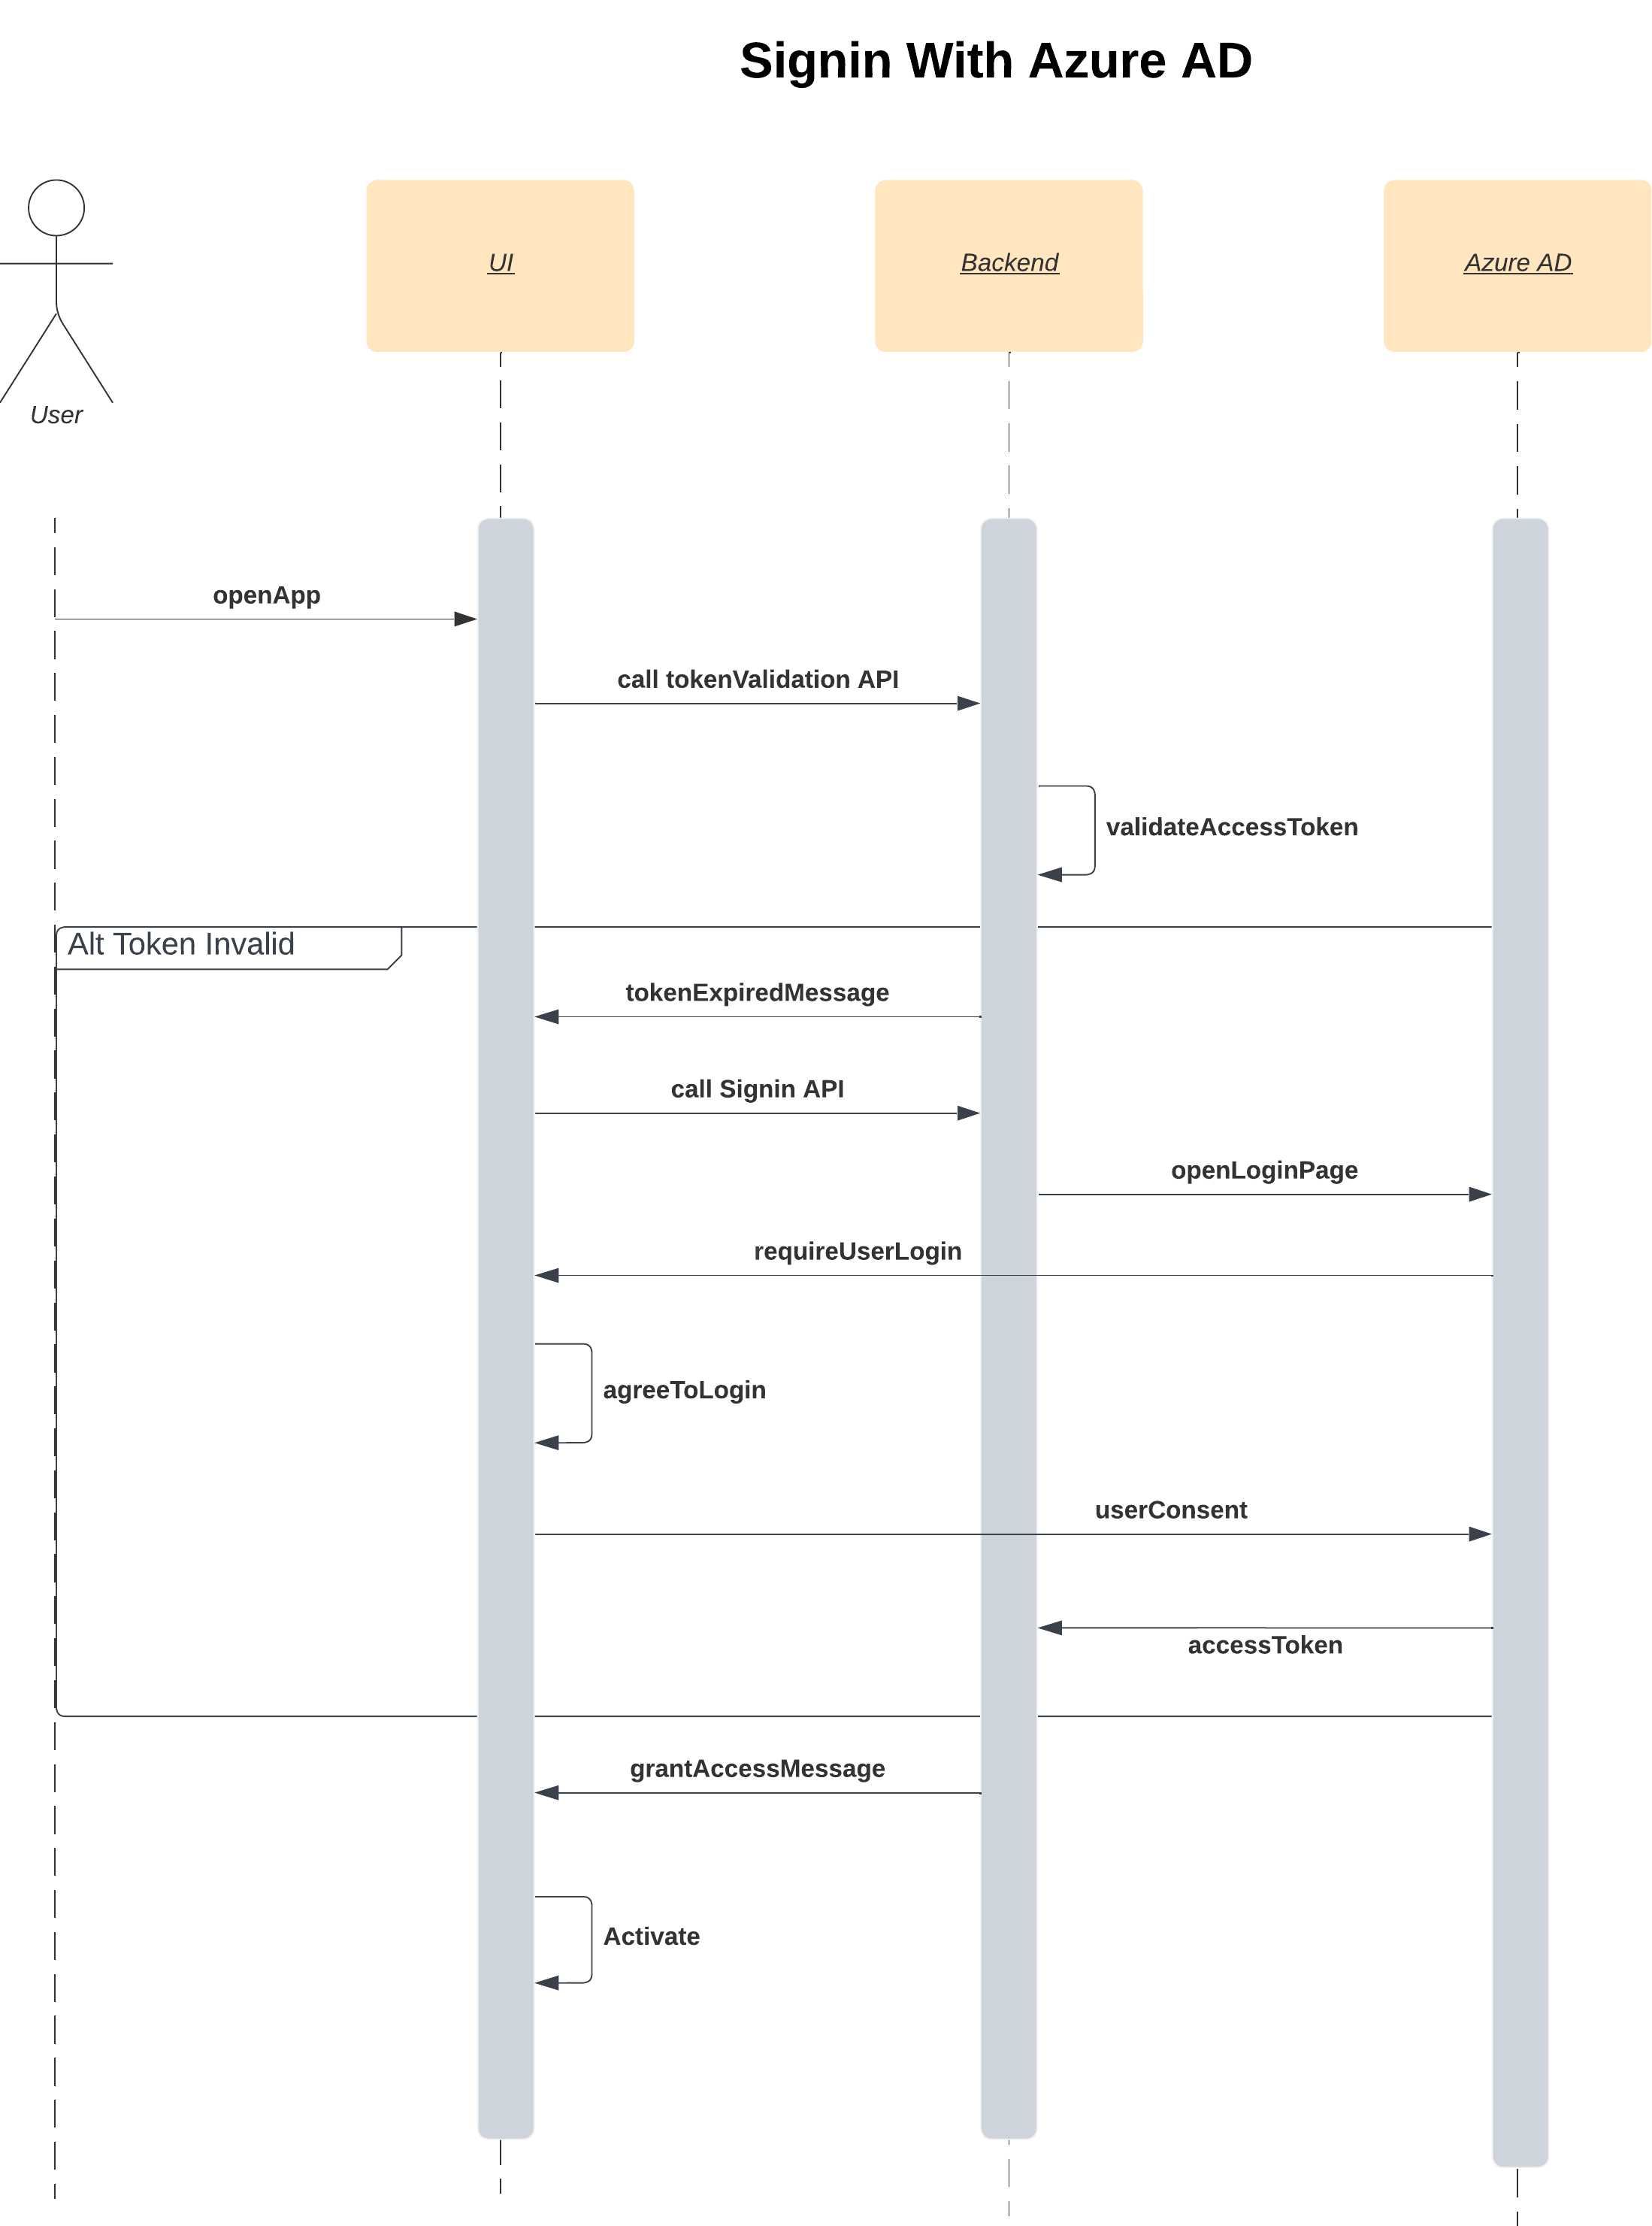
\includegraphics[width=13cm]{./Pictures/V5_Sequence_Diagram.png}}
    \caption{Edited Login Sequence Diagram}\label{fig:editedloginsequencediagram}
   \end{figure}
  \newpage
  ทางผู้จัดทําได้มีการปรับปรุงเเผนภาพที่ใช้เเสดงการทำงานของระบบ (Sequence Diagram) สำหรับกระบวนการการเข้าสู่ระบบ (Login) จากภาพที่ \ref{fig:regis} เป็นรูปที่ \ref{fig:editedloginsequencediagram} เนื่องด้วยเหตุผลสําคัญตามการเปลี่ยนแปลงที่ได้กล่าวไปในหัวข้อที่ \ref{subsec:editedfeaturelist} ทำให้กระบวนการเข้าสู่ระบบ (Login) และการพิสูจน์ยืนยันตัวตน (Authenticate) ของผู้ใช้งาน 
  จะเป็นการดําเนินการผ่านระบบ Microsoft Entra ID แทนการใช้ข้อมูลบัญชีสมาชิกที่ผู้ใช้งานจะต้องลงทะเบียนกับแอปพลิเคชันเพื่อเข้าใช้งานระบบของแอปพลิเคชัน และเนื่องจากไม่ต้องทำการลงทะเบียนกับแอปพลิเคชันแล้วจึงเป็นผลให้สามารถนําแผนภาพที่ \ref{fig:regis} ซึ่งเกี่ยวข้องกับการลงทะเบียนออกไปได้ เนื่องจากไม่มีความจําเป็นต่อการทํางานของระบบอีกต่อไป
  โดยแผนภาพ Sequence Diagram สำหรับกระบวนการการเข้าสู่ระบบ (Login) ที่ได้ทำการแก้ไขไปหรือรูปที่ \ref{fig:editedloginsequencediagram} นั้นแสดงลำดับการทำงานระหว่างองค์ประกอบต่าง ๆ ในระบบระหว่างกระบวนการเข้าสู่ระบบ (Login) และการพิสูจน์ยืนยันตัวตน (Authenticate) ของผู้ใช้งาน ซึ่งขั้นตอนการทำงานมีดังนี้:
  \begin{enumerate}
    \item ผู้ใช้เริ่มกระบวนการล็อกอินโดยเรียกใช้งานเปิดใช้งานแอปพลิเคชัน
    \item แอปพลิเคชันส่ง Request ที่ประกอบด้วย Access Token ไปยัง Backend System ผ่านการเรียกใช้งาน API สำหรับการตรวจสอบ Access Token
    \item Backend System ดำเนินการตรวจสอบความถูกต้องของ Access Token
    \item ดำเนินการตามสถานะจากการตรวจสอบ Access Token 
      \begin{enumerate}
        \item หาก Access Token ไม่ถูกต้อง จะทำการขอ Access Token ใหม่จาก Microsoft Entra ID โดยจะเป็นขั้นตอนตั้งแต่ข้อ 5 เป็นต้นไป 
        \item หาก Access Token ถูกต้องจะดำเนินการตามเข้าใช้งานแอปพลิเคชันตามปกติตามขั้นตอนที่ 18 เป็นต้นไป
      \end{enumerate}
    \item Backend System ส่ง Response กลับไปยังแอปพลิเคชันเพื่อแจ้งให้แอปพลิเคชันทราบว่า Access Token ไม่ถูกต้อง
    \item แอปพลิเคชันส่ง Request ไปยัง Backend System เพื่อขอ Login URL ผ่านการเรียกใช้งาน API สำหรับการขอ Login URL
    \item Backend System ส่ง Request ไปยัง Microsoft Entra ID เพื่อขอ Login URL
    \item Microsoft Entra ID ส่ง Login URL กลับไปยัง Backend System
    \item Backend System ส่ง Login URL กลับไปยังแอปพลิเคชัน
    \item แอปพลิเคชันเรียกใช้ Login URL เพื่อรองขอหน้า Login ของ Microsoft
    \item Microsoft Entra ID ส่งหน้า Login กลับไปยังแอปพลิเคชัน
    \item ผู้ใช้กรอกข้อมูลเข้าสู่ระบบในหน้า Login ของ Microsoft
    \item ผู้ใช้กดปุ่มเข้าสู่ระบบ
    \item Microsoft Entra ID สร้าง Access Token ใหม่และส่งกลับไปยัง Backend System
    \item Backend System ส่ง Access Token ไปยังแอปพลิเคชันเพื่อให้แอปพลิเคชันเรียกใช้งาน API ต่าง ๆ ในระบบ
    \item แอปพลิเคชันส่ง Request ที่ประกอบด้วย Access Token ไปยัง Backend System ผ่านการเรียกใช้งาน API สำหรับการตรวจสอบ Access Token อีกครั้ง
    \item Backend System ดำเนินการตรวจสอบความถูกต้องของ Access Token
    \item Backend System ส่ง Response กลับไปยังแอปพลิเคชันเพื่อแจ้งให้แอปพลิเคชันทราบว่า Access Token ถูกต้อง
    \item แอปพลิเคชันเริ่มใช้งานฟังก์ชันต่าง ๆ ในระบบได้
  \end{enumerate}
  \newpage
  \section{การพัฒนาของโครงการ}
  \begin{table}[!h]
    \centering
    \begin{tabular}{|l|c|c|}
    \hline
    \rowcolor[HTML]{9FC5E8} 
    \multicolumn{1}{|c|}{\cellcolor[HTML]{9FC5E8}รายการฟังก์ชันที่จะส่งมอบ}                                                                    & หลักฐาน & สถานะ      \\ \hline
    ระบบ Login ผ่านอีเมลของมหาวิทยาลัย                                                                                                         &         & กำลังพัฒนา \\ \hline
    \begin{tabular}[c]{@{}l@{}}ระบบรวบรวมข้อมูลของชมรมต่าง ๆ เอาไว้ โดยผู้ใช้สามารถค้นหาและ\\ ติดตามข้อมูลของชมรมที่ตนเองสนใจได้\end{tabular}   &         & กำลังพัฒนา \\ \hline
    ระบบแจ้งเตือนกิจกรรมที่เกี่ยวข้องกับชมรมหรือความสนใจของนักศึกษา                                                                             &         & กำลังพัฒนา \\ \hline
    ระบบแจ้งเตือนการประเมินผลกิจกรรม เมื่อฟอร์มการประเมินพร้อมใช้งาน                                                                            &         & กำลังพัฒนา \\ \hline
    \begin{tabular}[c]{@{}l@{}}ระบบแนะนํากิจกรรมและชมรม ตามความสนใจของผู้ใช้โดยอ้างอิง\\ จาก tag ของกิจกรรม\end{tabular}                        &         & กำลังพัฒนา \\ \hline
    \begin{tabular}[c]{@{}l@{}}ระบบวิเคราะห์ความสนใจของผู้ใช้ผ่านเนื้อหาของกิจกรรมที่ผู้ใช้เคยเข้าร่วม\\  เข้าไปอ่านรายละเอียด หรือเกี่ยวข้องกับชมรมที่สนใจ\end{tabular} &
       &
      กำลังพัฒนา \\ \hline
    \begin{tabular}[c]{@{}l@{}}ระบบแยกประเภทกิจกรรมอัตโนมัติโดยวิเคราะห์จากเนื้อหา \\ ออกมาเป็น tag ต่าง ๆ โดยใช้ Machine Learning\end{tabular} &         & กำลังพัฒนา \\ \hline
    \end{tabular}
    \captionof{table}{\centering ตารางการทดสอบการทดสอบการทํางาน}
  \end{table}
  \section{การทดสอบคุณภาพของระบบ (Non Functional Testing)}
Problem
\begin{itemize}
  \item คิดว่า Application นี้ตอบโจทย์กับปัญหาหรือไม่ ?
  \begin{table}[!h]
    \centering
    \captionsetup{justification=centering} % Set caption to be centered
    \begin{tabular}{|c|c|c|c|}
      \hline
      \multicolumn{1}{|c|}{\cellcolor[HTML]{9FC5E8}ระดับความพึงพอใจ} &
        \multicolumn{1}{c|}{\cellcolor[HTML]{9FC5E8}จำนวนผู้ให้คะแนน} \\ \hline
       1 &
         \\ \hline 
       2 &
         \\ \hline 
       3 &
         \\ \hline 
       4 &
         \\ \hline 
       5 &
         \\ \hline
    \end{tabular}
    \captionof{table}{\centering ตารางความพึงพอใจในการแก้ปัญหา}\label{tab:Problemssolvingsatisfaction}
  \end{table}
  \item มีข้อเสนอที่จะช่วยให้ Application นี้สมบูรณ์ขึ้นหรือไม่ ?
\end{itemize}
  Feature
\begin{itemize}
  \item Feature ที่ Application นี้ควรมีครบแล้วหรือยัง
  \begin{table}[!h]
    \centering
    \captionsetup{justification=centering} % Set caption to be centered
    \begin{tabular}{|c|c|c|c|}
      \hline
      \multicolumn{1}{|c|}{\cellcolor[HTML]{9FC5E8}ระดับความพึงพอใจ} &
        \multicolumn{1}{c|}{\cellcolor[HTML]{9FC5E8}จำนวนผู้ให้คะแนน} \\ \hline
       1 &
         \\ \hline 
       2 &
         \\ \hline 
       3 &
         \\ \hline 
       4 &
         \\ \hline 
       5 &
         \\ \hline
    \end{tabular}
    \captionof{table}{\centering ตารางความพึงพอใจของ Feature}\label{tab:Featuresatisfaction}
  \end{table}
  \item คิดว่า Application นี้ตอบโจทย์กับปัญหาหรือไม่ ?
\end{itemize}

\newpage

\section{การทดสอบการทำงาน (Functional Testing)}
\begin{table}[!h]
  \centering
  \captionsetup{justification=centering}
  \begin{tabular}{|l|p{3cm}|p{5cm}|p{3cm}|} 
  \hline
  \multicolumn{1}{|c|}{\cellcolor[HTML]{9FC5E8}Feature} & \multicolumn{1}{c|}{\cellcolor[HTML]{9FC5E8}Scenario} & \multicolumn{1}{c|}{\cellcolor[HTML]{9FC5E8}ผลที่คาดว่าจะได้รับ} & \multicolumn{1}{c|}{\cellcolor[HTML]{9FC5E8}ผลที่ได้รับ} \\
  \hline
  \multirow{4}{*}{Login} & ผู้ใช้งานไม่กรอกอีเมล หมายเลขโทรศัพท์ หรือชื่อ Skype ที่ถูกต้อง & ระบบ Microsoft Login แจ้งเตือน "ใส่ที่อยู่อีเมล หมายเลขโทรศัพท์ หรือชื่อ Skype ที่ถูกต้อง" & \\
  \cline{2-4} 
  & ผู้ใช้งานไม่กรอกรหัสผ่าน & ระบบ Microsoft Login แจ้งเตือน "โปรดป้อนรหัสผ่านของคุณ" & \\
  \cline{2-4}
  & ผู้ใช้งานกรอกอีเมลผิด & ระบบ Microsoft Login แจ้งเตือน "เราไม่พบบัญชีที่มีชื่อผู้ใช้ดังกล่าว" & \\
  \cline{2-4}
  & ผู้ใช้งานกรอกรหัสผ่านผิด & ระบบ Microsoft Login แจ้งเตือน "บัญชีหรือรหัสผ่านของคุณไม่ถูกต้อง" & \\
  \hline
  \multirow{2}{*}{Feed page} & ผู้ใช้งานกดดูรายละเอียดกิจกรรม & ระบบแสดงหน้ารายละเอียดของกิจกรรม & \\
  \cline{2-4}
  & ผู้ใช้งานกดดูรายละเอียดของชมรม & ระบบแสดงหน้ารายละเอียดของชมรม & \\
  \hline
  \multirow{2}{*}{Join Event} & ผู้ใช้งานกดเข้าร่วมกิจกรรม & ระบบแสดงหน้าจอว่าผู้ใช้ได้เข้าร่วมกิจกรรมแล้ว & \\
  \cline{2-4}
  & ผู้ใช้งานกดยกเลิกการเข้าร่วมกิจกรรม & \begin{tabular}[c]{@{}l@{}}ระบบแสดงหน้าจอว่าผู้ใช้ได้ยกเลิก\\การเข้าร่วมกิจกรรมแล้ว\end{tabular} & \\
  \hline
  \multirow{2}{*}{Join Club} & ผู้ใช้งานกดเข้าร่วมชมรม & ระบบแสดงหน้าจอว่าผู้ใช้ได้เข้าร่วมชมรมแล้ว & \\
  \cline{2-4}
  & ผู้ใช้งานกดยกเลิกการเข้าร่วมชมรม & ระบบแสดงหน้าจอว่าผู้ใช้ได้ยกเลิกการเข้าร่วมชมรมแล้ว & \\
  \hline
  Notification & ผู้ใช้กดเข้าไปดูแจ้งเตือนจากทางระบบ & \begin{tabular}[c]{@{}l@{}}ระบบแสดงหน้าจอเกี่ยวกับการแจ้งเตือนนั้น ๆ \\ เช่น ระบบแสดงหน้าจอการประเมินกิจกรรม\end{tabular} & \\
  \hline
  Evaluate Page & ผู้ใช้กดเพื่อเข้าไปประเมินกิจกรรม & ระบบพาผู้ใช้เข้าสู่หน้า login เพื่อประเมินกิจกรรม & \\
  \hline
  \end{tabular}
  \captionof{table}{\centering ตารางการทดสอบการทดสอบการทำงาน}\label{tab:functionaltesting}
  จากตารางที่ \ref{tab:functionaltesting} เป็นรายการสำหรับทดสอบการทำงานของฟังก์ชันต่าง ๆ ในแอพลิเคชัน เพื่อทดสอบว่าการตอบสนองต่อการใช้งานต่าง ๆ เป็นไปตามที่ออกแบบไว้หรือไม่
\end{table}

\section{ผลการทดสอบ (Test Results)}

\newpage
\chapter{สรุปผลการดำเนินงาน}
หลังจากการออกแบบ พัฒนา และทดสอบการทํางานของแอปพลิเคชันในบทที่ 4 ในบทที่ 5 นี้จะเป็นการกล่าวถึง
ผลสรุปการดำเนินงานของโครงการทั้งหมดตลอดปีการศึกษา 2023 ที่ผ่านมา โดยจะเป็นการสรุปผลกระบวนการทั้งที่ทางผู้จัดทำได้ทำสำเร็จไปแล้ว 
และกระบวนการที่ไม่สำเร็จ โดยรายละเอียดจะกล่าวตามแต่ละหัวข้อต่อไปนี้
\section{กระบวนการทำงาน (Work Process)}
\subsection{การดำเนินงานในภาคการศึกษาที่ 1}
  \subsubsection{การเตรียมการเริ่มต้นโครงการ}
  % Please add the following required packages to your document preamble:
  % \usepackage[table,xcdraw]{xcolor}
  % Beamer presentation requires \usepackage{colortbl} instead of \usepackage[table,xcdraw]{xcolor}
    \begin{table}[!h]\centering
      \begin{tabular}{|l|l|}
      \hline
      \rowcolor[HTML]{9FC5E8} 
      \multicolumn{1}{|c|}{\cellcolor[HTML]{9FC5E8}ภาระงาน} & \multicolumn{1}{c|}{\cellcolor[HTML]{9FC5E8}สถานะงาน} \\ \hline
      จัดทำ Idea Document                                 & \cellcolor[HTML]{34FF34}เสร็จสิ้น                        \\ \hline
      จัดทำ Project Proposal                              & \cellcolor[HTML]{34FF34}เสร็จสิ้น                        \\ \hline
      จัดทำแผนการดำเนินงานของโครงการ                      & \cellcolor[HTML]{34FF34}เสร็จสิ้น                        \\ \hline
      \end{tabular}
      \end{table}

  \subsubsection{ศึกษาวิธีการพัฒนาแอปพลิเคชัน}
    \begin{table}[!h]\centering
      \begin{tabular}{|l|l|}
      \hline
      \rowcolor[HTML]{9FC5E8} 
      \multicolumn{1}{|c|}{\cellcolor[HTML]{9FC5E8}ภาระงาน} & \multicolumn{1}{c|}{\cellcolor[HTML]{9FC5E8}สถานะงาน} \\ \hline
      ศึกษาวิธีการพัฒนาแอปพลิเคชันส่วน Front-end          & \cellcolor[HTML]{34FF34}เสร็จสิ้น                        \\ \hline
      ศึกษาวิธีการพัฒนาแอปพลิเคชันส่วน Back-end              & \cellcolor[HTML]{34FF34}เสร็จสิ้น                        \\ \hline
      ศึกษาวิธีการพัฒนาฐานข้อมูล                          & \cellcolor[HTML]{34FF34}เสร็จสิ้น                        \\ \hline
      ศึกษาวิธีการพัฒนา Machine Learning                  & \cellcolor[HTML]{34FF34}เสร็จสิ้น                        \\ \hline
      \end{tabular}
      \end{table}

  \subsubsection{ออกแบบแอปพลิเคชัน}
    \begin{table}[!h]\centering
      \begin{tabular}{|l|l|}
      \hline
      \rowcolor[HTML]{9FC5E8} 
      \multicolumn{1}{|c|}{\cellcolor[HTML]{9FC5E8}ภาระงาน} & \multicolumn{1}{c|}{\cellcolor[HTML]{9FC5E8}สถานะงาน} \\ \hline
      จัดทำ Architecture Diagram                          & \cellcolor[HTML]{34FF34}เสร็จสิ้น                        \\ \hline
      จัดทำ Use Case Diagram                              & \cellcolor[HTML]{34FF34}เสร็จสิ้น                        \\ \hline
      จัดทำ Sequence Diagram                              & \cellcolor[HTML]{34FF34}เสร็จสิ้น                        \\ \hline
      จัดทำ Database Schema                               & \cellcolor[HTML]{34FF34}เสร็จสิ้น                        \\ \hline
      จัดทำ Application Wireframe                         & \cellcolor[HTML]{34FF34}เสร็จสิ้น                        \\ \hline
      จัดทำ Application UX/UI                             & \cellcolor[HTML]{34FF34}เสร็จสิ้น                        \\ \hline
      \end{tabular}
      \end{table}
      
  \subsubsection{จัดเตรียมข้อมูล}
    \begin{table}[!h]\centering
      \begin{tabular}{|l|l|}
      \hline
      \rowcolor[HTML]{9FC5E8} 
      \multicolumn{1}{|c|}{\cellcolor[HTML]{9FC5E8}ภาระงาน} & \multicolumn{1}{c|}{\cellcolor[HTML]{9FC5E8}สถานะงาน} \\ \hline
      Data Preprocessing                & \cellcolor[HTML]{34FF34}เสร็จสิ้น                        \\ \hline
      \end{tabular}
      \end{table}
  
  จากตารางข้างต้น เป็นตารางสรุปภาระงานและสถานะงานที่ทางทีมพัฒนาได้ดำเนินการไปในภาคการศึกษาที่ 1 โดยภาระงานที่ทางทีมพัฒนาได้วางแผนไว้ในภาคการศึกษานี้จะเป็นการเตรียมความพร้อมสำหรับการพัฒนาแอปพลิเคชันในภาคการศึกษาที่ 2 
  และจากข้อมูลภายในตาราง สามารถสรุปได้ว่าทางผู้จัดทำได้ดำเนินการจัดการทุกภาระงานจนเสร็จสิ้นตามแผนการดำเนินงานที่กำหนดไว้เป็นที่เรียบร้อย
\subsection{การดำเนินงานในภาคการศึกษาที่ 2}
  \subsubsection{การพัฒนาแอปพลิเคชัน}
    \begin{table}[H]\centering
      \begin{tabular}{|l|l|}
      \hline
      \rowcolor[HTML]{9FC5E8} 
      \multicolumn{1}{|c|}{\cellcolor[HTML]{9FC5E8}ภาระงาน} & \multicolumn{1}{c|}{\cellcolor[HTML]{9FC5E8}สถานะงาน} \\ \hline
      พัฒนาแอปพลิเคชันส่วน Front-end                                 & \cellcolor[HTML]{F8FF00}กำลังดำเนินการ                        \\ \hline
      พัฒนาแอปพลิเคชันส่วน Back-end                              & \cellcolor[HTML]{F8FF00}กำลังดำเนินการ                        \\ \hline
      พัฒนาฐานข้อมูล                      & \cellcolor[HTML]{F8FF00}กำลังดำเนินการ                        \\ \hline
      พัฒนา Machine Learning          & \cellcolor[HTML]{F8FF00}กำลังดำเนินการ                        \\ \hline
      \end{tabular}
      \end{table}
      
    \subsubsection{การทดสอบแอปพลิเคชัน}
      \begin{table}[H]\centering
        \begin{tabular}{|l|l|}
        \hline
        \rowcolor[HTML]{9FC5E8} 
        \multicolumn{1}{|c|}{\cellcolor[HTML]{9FC5E8}ภาระงาน} & \multicolumn{1}{c|}{\cellcolor[HTML]{9FC5E8}สถานะงาน} \\ \hline
        ออกแบบ Test Cases              & \cellcolor[HTML]{F8FF00}กำลังดำเนินการ                        \\ \hline
        ทดสอบการทำงานของแอปพลิเคชัน (Functional Testing)              & \cellcolor[HTML]{C0C0C0}ยังไม่ได้ดำเนินการ                        \\ \hline
        ทดสอบคุณภาพของระบบ (Non Functional Testing)                  & \cellcolor[HTML]{C0C0C0}ยังไม่ได้ดำเนินการ                        \\ \hline
        \end{tabular}
        \end{table}
  จากตารางข้างต้น เป็นตารางสรุปภาระงานและสถานะงานที่ทางทีมพัฒนาวางแผนจะดำเนินการในภาคการศึกษาที่ 2 โดยภาระงานที่ทางทีมพัฒนาได้วางแผนไว้ในภาคการศึกษานี้จะเป็นการพัฒนาแอปพลิเคชันตามแผนที่ได้เตรียมการไว้ในภาคการศึกษาที่ 1
  โดยสถานะของภาระงานส่วนใหญ่ยังอยู่ในขั้นตอนการดำเนินการ
\section{ปัญหาที่พบในโครงการและการแก้ไข (Problems and Solutions)}
\subsection{ความไม่คุ้นชินกับเทคโนโลยีที่ใช้ในการพัฒนา}
เนื่องจากคณะผู้จัดทำแต่ล่ะคนมีความถนัดในเทคโนโลยีที่แตกต่างกัน และในแต่ล่ะเทคโนโลยีที่ใช้ในการพัฒนาโครงการนั้นผู้จัดทำแต่ล่ะคนก็มีความเชี่ยวชาญที่ไม่เท่ากัน 
จึงเกิดเป็นอุปสรรคในการทำงานเนื่องจากความไม่คุ้นเคยกับเทคโนโลยีที่ถูกหยิบมาใช้งานในการพัฒนาโครงการ
\subsection{จำนวนข้อมูลที่สามารถใช้ได้มีน้อย}
ข้อมูลกิจกรรมนักศึกษาของทางมหาวิทยาลัยเทคโนโลยีพระจอมเกล้าธนบุรีที่ถูกบันทึกเอาไว้ในระบบนั้นมีย้อนไปถึงเพียงปีการศึกษาที่ 2558 เท่านั้น 
รวมจำนวนกิจกรรมที่บันทึกได้อยู่ 2565 รายการ ซึ่งเป็นจำนวนที่น้อยเมื่อต้องใช้ในการเทรนโมเดลการเรียนรู้ของเครื่อง ซึ่งจำเป็นต้องใช้ Tranfer Learning 
เพื่อดึงค่าน้ำหนักของโมเดลที่มีการเทรนไว้ก่อนแล้วมาพัฒนาต่อเพื่อให้ได้โมเดลที่สามารถให้ผลลัพธ์ที่เหมาะสมออกมาได้
\subsection{ความลำบากในการขอข้อมูลจากมหาวิทยาลัย}
เนื่องจากหน่วยงานที่เป็นเจ้าของข้อมูลที่ใช้ในการพัฒนาโครงการนั้นเป็นหน่วยงานที่มีงานในการดำเนินงานตลอดเวลา จึงมีความลำบากในการติดต่อเพื่อเข้าไปขอใช้ข้อมูล
\subsection{หน่วยประมวลผลที่ใช้ในการพัฒนา Machine Learning มีจำนวนน้อย}
ในการเทรนโมเดลการเรียนรู้ของเครื่องนั้นต้องอาศัยหน่วยประมวลผลจำนวนมากในการเทรน ซึ่งด้วยหน่วยประมวลผลที่เข้าถึงได้แบบไม่มีค่าใช้จ่ายนั้นมีไม่เพียงพอต่อการพัฒนาโมเดลอย่างมีประสิทธิภาพ
\section{แนวทางการพัฒนาในอนาคต (Future Work)}
\makeatletter
\g@addto@macro{\UrlBreaks}{\UrlOrds}
\makeatother

\bibliographystyle{kmutt}
\bibliography{string,cpe}

\end{document}